\documentclass[10pt,a4paper]{article}
\usepackage[margin=2cm]{geometry}
\usepackage{amsmath,amssymb,amsthm}
\usepackage[T1]{fontenc}
\usepackage[utf8]{inputenc}
\DeclareUnicodeCharacter{2192}{\ensuremath{\to}}
\DeclareUnicodeCharacter{2194}{\ensuremath{\leftrightarrow}}
\DeclareUnicodeCharacter{2261}{\ensuremath{\equiv}}
\DeclareUnicodeCharacter{2282}{\ensuremath{\subset}}
\DeclareUnicodeCharacter{03C3}{\ensuremath{\sigma}}
\DeclareUnicodeCharacter{00B7}{\ensuremath{\cdot}}
\DeclareUnicodeCharacter{2014}{---}
\DeclareUnicodeCharacter{2013}{--}
\DeclareUnicodeCharacter{2019}{'}
\DeclareUnicodeCharacter{00D7}{\ensuremath{\times}}

\usepackage{lmodern}
\usepackage{xcolor}
\usepackage{tikz}
\usetikzlibrary{arrows.meta}
\usepackage{hyperref}
\hypersetup{colorlinks=true, linkcolor=black, urlcolor=blue!50!black}
\definecolor{acol}{HTML}{2F86A6}
\definecolor{bcol}{HTML}{C97E1C}
\definecolor{netc}{HTML}{4F8A3C}
\definecolor{residc}{HTML}{8E8478}
\definecolor{latfill}{HTML}{EEF6F2}
\newcommand{\nest}{\preceq}
\newcommand{\nnest}{\not\preceq}
\newtheorem*{lemma}{Lemma}
\setlength{\parindent}{0pt}
\setlength{\parskip}{3pt}

\title{SEMNEST: proofs of the nesting and equivalence relations\\[4pt]\large all 80 items of the capsule}
\author{Generated with the capsule's item bank (\texttt{bank.js}) and checked in exact arithmetic\\ (\texttt{.dev/proofs/build.js}); see also \texttt{.dev/verify\_bank.js} and \texttt{.dev/verify\_bank.R}}
\date{}

\begin{document}
\maketitle

\section*{1\quad Setting and definitions}

Each item compares two models, $A$ (left) and $B$ (right), for the same $p$ observed variables. A model is written in RAM form
\[
v = \mathbf A v + u,\qquad \mathrm{Cov}(u)=\mathbf S,\qquad \Sigma_{\text{full}}=(I-\mathbf A)^{-1}\mathbf S(I-\mathbf A)^{-\top},
\]
with $v$ the observed and latent variables and $\Sigma$ the observed block of $\Sigma_{\text{full}}$. $\mathbf A$ holds the drawn directed effects (loadings $\lambda$, regressions $\beta$, second-order loadings $\gamma$); $\mathbf S$ holds a free variance for every variable (the residual variance $\theta_{ii}$ or $\psi$ of an endogenous variable) and the drawn covariances. For variables in a \emph{network block}, the block of $\mathbf S$ is $K^{-1}$, where the precision matrix $K$ has a free diagonal and free off-diagonal elements only for the drawn undirected edges: a Gaussian graphical model (GGM) on observed variables, a residual network model (RNM) on the residuals of indicators, or a latent network model (LNM) on latent variables (Epskamp, Rhemtulla \& Borsboom, 2017, \emph{Psychometrika}).

\textbf{Parameters.} The free parameters $\theta\in\mathbb R^{q}$ are unrestricted real numbers: variances may be negative (Heywood solutions), as in lavaan's default estimation. The scale of each latent variable is fixed by its first loading (marker variable); $q_X$ counts the free parameters of model $X$. Let $\Theta_X=\{\theta:\Sigma_X(\theta)\text{ exists and is positive definite}\}$ (an open set) and
\[
\mathcal M_X=\{\Sigma_X(\theta):\theta\in\Theta_X\},
\]
the set of covariance matrices model $X$ can produce. $\overline{\mathcal M}$ denotes the closure within the positive definite matrices.

\textbf{Definition.} $X$ is \emph{nested} in $Y$, written $X\nest Y$, if $\mathcal M_X\subseteq\overline{\mathcal M_Y}$: every covariance matrix that $X$ can produce, $Y$ can produce or approximate arbitrarily closely, so fitting $Y$ to it gives a perfect fit ($F_{\mathrm{ML}}=0$, $\chi^2=0$). This is exactly what the numerical check of Bentler \& Satorra (2010) and of the PL5225 assignment tests. $X$ and $Y$ are \emph{equivalent} ($X\equiv Y$) if $X\nest Y$ and $Y\nest X$. \emph{$A$ is nested in $B$} in the game means $A\nest B$ and $B\nnest A$; \emph{neither} means $A\nnest B$ and $B\nnest A$.

The closure makes the definition insensitive to the measure-zero exceptions that are typical for latent variable models (e.g.\ a mapping that divides by a covariance that happens to be zero). Allowing negative variances is what makes the textbook statements (``a one-factor model with three indicators is saturated'', ``a second-order factor on three factors is equivalent to three correlated factors'') literally true.

\section*{2\quad Lemmas}

\begin{lemma}[R, restriction]
If $X$ is obtained from $Y$ by fixing free parameters of $Y$ to constants or by equating them, then $X\nest Y$.
\end{lemma}
\emph{Proof.} $\Theta_X$ embeds in $\Theta_Y$ with the same implied $\Sigma$. \qed

\begin{lemma}[G, generic maps]
If there are a dense subset $D\subseteq\Theta_X$ and a map $\varphi:D\to\Theta_Y$ with $\Sigma_Y(\varphi(\theta))=\Sigma_X(\theta)$ for all $\theta\in D$, then $X\nest Y$.
\end{lemma}
\emph{Proof.} $\Sigma_X$ is continuous, so $\mathcal M_X=\Sigma_X(\Theta_X)\subseteq\overline{\Sigma_X(D)}\subseteq\overline{\mathcal M_Y}$. In the items $D$ is $\Theta_X$ minus the zero set of a polynomial that is not identically zero (``generic'' parameter values), which is dense. \qed

\begin{lemma}[S, separating constraint]
If a polynomial $f$ in the entries of $\Sigma$ vanishes on $\mathcal M_Y$ and $f(\Sigma_X(\theta^*))\neq0$ for some $\theta^*\in\Theta_X$, then $X\nnest Y$.
\end{lemma}
\emph{Proof.} $f$ is continuous, so it vanishes on $\overline{\mathcal M_Y}$, which therefore does not contain $\Sigma_X(\theta^*)$. \qed

In every application below, $f$ vanishing on $\mathcal M_Y$ is shown algebraically in the text (and was also checked in exact rational arithmetic at random rational parameter values), and the point $\theta^*$ with rational coordinates is listed in Appendix~B together with the exact value of $f$.

\begin{lemma}[D, dimension]
Let $J_X(\theta)$ be the Jacobian of $\theta\mapsto\operatorname{vech}\Sigma_X(\theta)$. If $\operatorname{rank}J_X(\theta^*)>q_Y$ for some $\theta^*\in\Theta_X$, then $X\nnest Y$.
\end{lemma}
\emph{Proof.} $\mathcal M_Y$ is the image of a semialgebraic set of dimension $q_Y$ under a rational map, so $\overline{\mathcal M_Y}$ is semialgebraic with dimension at most $q_Y$. The rank of $J_X$ is lower semicontinuous, so its maximum $r\ge\operatorname{rank}J_X(\theta^*)>q_Y$ is attained on a nonempty open subset of $\Theta_X$, where the rank is constant; by the constant rank theorem $\mathcal M_X$ contains an $r$-dimensional embedded submanifold, which cannot lie in a semialgebraic set of dimension $<r$. \qed

The ranks were computed exactly (rational arithmetic) at the rational points listed in Appendix~B.

\begin{lemma}[B, saturated blocks]
(a) The following are saturated ($\overline{\mathcal M}$ = all positive definite matrices): the model with all covariances free; a complete recursive path model (every pair connected by a directed path following a fixed order); a one-factor model with three indicators. (b) If two models differ only in how they model the covariance matrix of a block of variables that is connected to the rest of the model in the same way, and both can produce every covariance matrix of that block (up to closure), the models are equivalent; if only one of them can, the other is nested in it.
\end{lemma}
\emph{Proof.} (a) Every $\Sigma\succ0$ has a Cholesky factorization $\Sigma=(I-B)^{-1}D(I-B)^{-\top}$ with $B$ strictly lower triangular and $D$ diagonal; that is a complete recursive path model. For one factor with three indicators and $\sigma_{12}\sigma_{13}\sigma_{23}\neq0$: $\lambda_1=1$, $\psi=\sigma_{12}\sigma_{13}/\sigma_{23}$, $\lambda_2=\sigma_{23}/\sigma_{13}$, $\lambda_3=\sigma_{23}/\sigma_{12}$, $\theta_{ii}=\sigma_{ii}-\lambda_i^2\psi$ reproduce $\Sigma$; apply Lemma~G. (b) The implied $\Sigma$ depends on the block only through the block's covariance matrix (e.g.\ $\Sigma=\Lambda\Psi\Lambda^\top+\Theta$ for the latent block). \qed

\begin{lemma}[M, merging factors]
In a factor model where the covariance matrix $\Psi$ of the factors is free, setting the variances and covariances of factors $F_k$ and $F_l$ equal ($\psi_{kk}=\psi_{ll}=\psi_{kl}$ and $\psi_{km}=\psi_{lm}$ for all other $m$) makes $F_k=F_l$ almost surely. Hence the model in which $F_k$ and $F_l$ are replaced by one factor loading on the union of their indicators is nested in it.
\end{lemma}
\emph{Proof.} With these values $\mathrm{Var}(F_k-F_l)=0$; the implied $\Sigma$ is that of the merged model (Lemma~R on the parameters). \qed

\begin{lemma}[P, pairs]
Let $F$ be a latent variable of model $X$ and $y_i,y_j$ two observed variables whose only paths are loadings from $F$. Let $X^{+}$ be $X$ plus the residual covariance $y_i\leftrightarrow y_j$, and $X^{G}$ be $X$ in which $y_i,y_j$ instead load on a new latent variable $G$ whose only path is $F\to G$. Then $X^{+}\equiv X^{G}$.
\end{lemma}
\emph{Proof.} In $X^G$ write $G=\gamma F+u$ with $u$ independent of all other variables. Then $y_i=\lambda^G_i\gamma F+\lambda^G_iu+e_i$, and likewise for $y_j$: this is $X^{+}$ with loadings $\lambda_i=\lambda^G_i\gamma$, $\lambda_j=\lambda^G_j\gamma$, residual covariance $\theta_{ij}=\lambda^G_i\lambda^G_j\mathrm{Var}(u)$ and residual variances $\theta_{ii}+(\lambda^G_i)^2\mathrm{Var}(u)$; nothing else changes. Conversely, given $X^{+}$ with $\lambda_i\lambda_j\neq0$, take $\gamma=1$, $\lambda^G_i=\lambda_i$, $\lambda^G_j=\lambda_j$, $\mathrm{Var}(u)=\theta_{ij}/(\lambda_i\lambda_j)$ (possibly negative) and residual variances $\theta_{ii}-\lambda_i^2\mathrm{Var}(u)$. Lemma~G gives both directions. \qed

Note that if $F$ is exogenous and $G$ has no other paths, $F\to G$ and $F\leftrightarrow G$ give the same (saturated) $2\times2$ latent block, so by Lemma~B(b) $G$ may also simply be a factor correlated with $F$.

\begin{lemma}[I, inverses]
For a positive definite $\Sigma$, $(\Sigma^{-1})_{ij}=0$ iff the partial covariance of $i$ and $j$ given all other variables is $0$. $\Sigma$ is block-diagonal iff $\Sigma^{-1}$ is block-diagonal (with the same blocks). For three variables, $(\Sigma^{-1})_{13}=0$ iff $\sigma_{12}\sigma_{23}-\sigma_{13}\sigma_{22}=0$.
\end{lemma}
\emph{Proof.} Standard: $(\Sigma^{-1})_{ij}=C_{ji}/\det\Sigma$ with $C$ the cofactor matrix; the inverse of a block-diagonal matrix is block-diagonal; for $3\times3$, $C_{31}=\sigma_{12}\sigma_{23}-\sigma_{13}\sigma_{22}$. \qed

\begin{lemma}[C, trees]
Let a path model be a DAG whose skeleton is a tree and in which no variable has two parents (no colliders: chains and forks). Then its set of covariance matrices equals the GGM on the skeleton, $\{\Sigma\succ0:(\Sigma^{-1})_{ij}=0\text{ for every non-adjacent pair}\}$.
\end{lemma}
\emph{Proof.} For a DAG, $\Sigma^{-1}=(I-B)^\top D^{-1}(I-B)$ with $B$ supported on the arrows. If every node has at most one parent, $\big((I-B)^\top D^{-1}(I-B)\big)_{ij}$ for $i\neq j$ is nonzero only if $i$ is the parent of $j$ or vice versa (a product term $b_{ki}b_{kj}$ would need a common child $k$ with two parents). So the DAG is contained in the GGM. Conversely, a $\Sigma\succ0$ with tree-shaped inverse factorizes along any orientation of the tree away from a root (the Gaussian density factorizes over a tree as $\prod_k p(x_k\mid x_{\mathrm{pa}(k)})$; see Lauritzen, 1996), and every collider-free orientation of a tree points away from some root. \qed

\begin{lemma}[T, perfect indicators]
In a factor model, an indicator $y_1$ of $F$ with $\theta_{11}=0$ and $\lambda_1=1$ equals $F$. Hence the path model in which $y_1$ is an exogenous cause of the other indicators of $F$ ($y_k=\lambda_ky_1+e_k$) is nested in the factor model.
\end{lemma}
\emph{Proof.} Take $\theta_{11}=0$ (allowed: parameters are unrestricted) and $\psi=\mathrm{Var}(y_1)$; Lemma~R. \qed

\begin{lemma}[H, higher-order and bifactor; Yung, Thissen \& McLeod, 1999]
A higher-order model (first-order factors $F_k$ with disjoint indicator sets, $F_k=\gamma_kG+\zeta_k$) is nested in the bifactor model with a general factor on all indicators and one orthogonal group factor per first-order factor.
\end{lemma}
\emph{Proof.} For an indicator $y_i$ of $F_k$: $y_i=\lambda_i\gamma_kG+\lambda_i\zeta_k+e_i$. The general factor $G$ and the disturbances $\zeta_k$ are mutually uncorrelated, so this is a bifactor model with general loadings $\lambda_i\gamma_k$, group factor $S_k=\zeta_k$ with loadings $\lambda_i$ and variance $\mathrm{Var}(\zeta_k)$ (possibly negative). Rescale $G$ to its marker loading (generic: $\lambda_{1}\gamma_1\neq0$). \qed

\section*{3\quad How to read an item page}
Each page shows the two path diagrams exactly as in the game (observed variables as squares, latent variables as circles, residuals as small circles, covariances as curved double-headed arrows, network edges as green lines; variances are free and not drawn), the model syntax ($\sim\sim$ is a covariance, \texttt{--} a network edge, \texttt{network} lists a network block, \texttt{a*} an equality label), the claim and its proof. (i) concerns $A\nest B$, (ii) concerns $B\nest A$. $\sigma_{ij}$ is the covariance of $y_i$ and $y_j$.

\tableofcontents

\clearpage
\section*{E01 \quad Chain versus fork}
\addcontentsline{toc}{subsection}{E01\quad Chain versus fork}
\noindent\textit{Level: Easy.} Observed variables: $A, B, C$ ($p=3$, 6 moments).\par\medskip
\noindent\begin{minipage}[t]{0.49\textwidth}\centering\textbf{\color{acol}Model A} \;{\small $q_A=5$}\\[2pt]
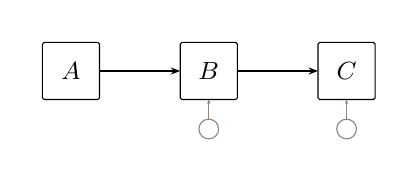
\begin{tikzpicture}[x=1cm, y=1cm,
    obs/.style={draw, rounded corners=0.6pt, minimum size=0.725cm, inner sep=0pt, fill=white, font=\fontsize{9.0}{10}\selectfont},
    lat/.style={draw, circle, minimum size=0.900cm, inner sep=0pt, fill=latfill, font=\fontsize{9.0}{10}\selectfont},
    resid/.style={draw=residc, line width=0.4pt}, residarrow/.style={draw=residc, -{Stealth[length=1.6pt]}, line width=0.4pt},
    path/.style={-{Stealth[length=3.4pt]}, line width=0.55pt},
    cov/.style={{Stealth[length=3.4pt]}-{Stealth[length=3.4pt]}, line width=0.55pt},
    net/.style={draw=netc, line width=1.1pt, line cap=round},
    elabel/.style={font=\scriptsize\itshape, fill=white, inner sep=0.6pt}]
\useasboundingbox (-0.550,0.550) rectangle (4.050,-1.050);
\draw[resid] (1.750,-0.737) circle (0.125);
\draw[residarrow] (1.750,-0.613) -- (1.750,-0.362);
\draw[resid] (3.500,-0.737) circle (0.125);
\draw[residarrow] (3.500,-0.613) -- (3.500,-0.362);
\draw[path] (0.362,0.000) -- (1.387,0.000);
\draw[path] (2.112,0.000) -- (3.137,0.000);
\node[obs] at (0.000,0.000) {$A$};
\node[obs] at (1.750,0.000) {$B$};
\node[obs] at (3.500,0.000) {$C$};
\end{tikzpicture}\\[1pt]{\scriptsize \texttt{B \char`\~{} A; C \char`\~{} B}}\end{minipage}\hfill
\begin{minipage}[t]{0.49\textwidth}\centering\textbf{\color{bcol}Model B} \;{\small $q_B=5$}\\[2pt]
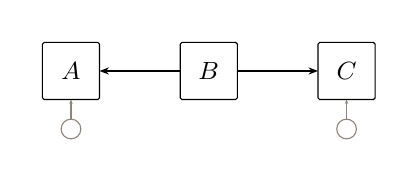
\begin{tikzpicture}[x=1cm, y=1cm,
    obs/.style={draw, rounded corners=0.6pt, minimum size=0.725cm, inner sep=0pt, fill=white, font=\fontsize{9.0}{10}\selectfont},
    lat/.style={draw, circle, minimum size=0.900cm, inner sep=0pt, fill=latfill, font=\fontsize{9.0}{10}\selectfont},
    resid/.style={draw=residc, line width=0.4pt}, residarrow/.style={draw=residc, -{Stealth[length=1.6pt]}, line width=0.4pt},
    path/.style={-{Stealth[length=3.4pt]}, line width=0.55pt},
    cov/.style={{Stealth[length=3.4pt]}-{Stealth[length=3.4pt]}, line width=0.55pt},
    net/.style={draw=netc, line width=1.1pt, line cap=round},
    elabel/.style={font=\scriptsize\itshape, fill=white, inner sep=0.6pt}]
\useasboundingbox (-0.550,0.550) rectangle (4.050,-1.050);
\draw[resid] (0.000,-0.737) circle (0.125);
\draw[residarrow] (0.000,-0.613) -- (0.000,-0.362);
\draw[resid] (3.500,-0.737) circle (0.125);
\draw[residarrow] (3.500,-0.613) -- (3.500,-0.362);
\draw[path] (1.387,0.000) -- (0.362,0.000);
\draw[path] (2.112,0.000) -- (3.137,0.000);
\node[obs] at (0.000,0.000) {$A$};
\node[obs] at (1.750,0.000) {$B$};
\node[obs] at (3.500,0.000) {$C$};
\end{tikzpicture}\\[1pt]{\scriptsize \texttt{A \char`\~{} B; C \char`\~{} B}}\end{minipage}
\par\bigskip
\noindent\textbf{Claim.} $A \equiv B$: the models are \textbf{equivalent}.\par\smallskip
\noindent\textbf{Proof.} (i) $A\nest B$. Both graphs have the skeleton $A - B - C$ and no collider, so by Lemma~C both models equal the GGM with $(\Sigma^{-1})_{AC}=0$, i.e.\ $\mathcal M=\{\Sigma\succ0:\sigma_{AC}\sigma_{BB}=\sigma_{AB}\sigma_{BC}\}$.\par\smallskip
\noindent(ii) $B\nest A$. See the previous line: $\mathcal M_A=\mathcal M_B$.\hfill$\square$\par\medskip
\noindent{\small\textit{In the game:} Both models say that A and C are unrelated once you know B. Turning the first arrow around does not change that, so both reproduce exactly the same covariance matrices.}

\clearpage
\section*{E02 \quad A chain and its reverse}
\addcontentsline{toc}{subsection}{E02\quad A chain and its reverse}
\noindent\textit{Level: Easy.} Observed variables: $A, B, C, D$ ($p=4$, 10 moments).\par\medskip
\noindent\begin{minipage}[t]{0.49\textwidth}\centering\textbf{\color{acol}Model A} \;{\small $q_A=7$}\\[2pt]
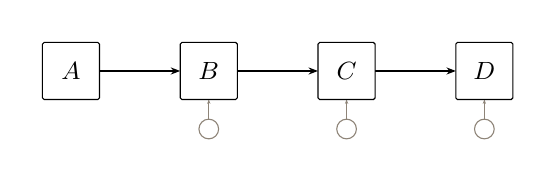
\begin{tikzpicture}[x=1cm, y=1cm,
    obs/.style={draw, rounded corners=0.6pt, minimum size=0.725cm, inner sep=0pt, fill=white, font=\fontsize{9.0}{10}\selectfont},
    lat/.style={draw, circle, minimum size=0.900cm, inner sep=0pt, fill=latfill, font=\fontsize{9.0}{10}\selectfont},
    resid/.style={draw=residc, line width=0.4pt}, residarrow/.style={draw=residc, -{Stealth[length=1.6pt]}, line width=0.4pt},
    path/.style={-{Stealth[length=3.4pt]}, line width=0.55pt},
    cov/.style={{Stealth[length=3.4pt]}-{Stealth[length=3.4pt]}, line width=0.55pt},
    net/.style={draw=netc, line width=1.1pt, line cap=round},
    elabel/.style={font=\scriptsize\itshape, fill=white, inner sep=0.6pt}]
\useasboundingbox (-0.550,0.550) rectangle (5.800,-1.050);
\draw[resid] (1.750,-0.737) circle (0.125);
\draw[residarrow] (1.750,-0.613) -- (1.750,-0.362);
\draw[resid] (3.500,-0.737) circle (0.125);
\draw[residarrow] (3.500,-0.613) -- (3.500,-0.362);
\draw[resid] (5.250,-0.737) circle (0.125);
\draw[residarrow] (5.250,-0.613) -- (5.250,-0.362);
\draw[path] (0.362,0.000) -- (1.387,0.000);
\draw[path] (2.112,0.000) -- (3.137,0.000);
\draw[path] (3.862,0.000) -- (4.888,0.000);
\node[obs] at (0.000,0.000) {$A$};
\node[obs] at (1.750,0.000) {$B$};
\node[obs] at (3.500,0.000) {$C$};
\node[obs] at (5.250,0.000) {$D$};
\end{tikzpicture}\\[1pt]{\scriptsize \texttt{B \char`\~{} A; C \char`\~{} B; D \char`\~{} C}}\end{minipage}\hfill
\begin{minipage}[t]{0.49\textwidth}\centering\textbf{\color{bcol}Model B} \;{\small $q_B=7$}\\[2pt]
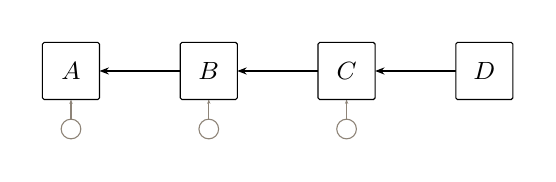
\begin{tikzpicture}[x=1cm, y=1cm,
    obs/.style={draw, rounded corners=0.6pt, minimum size=0.725cm, inner sep=0pt, fill=white, font=\fontsize{9.0}{10}\selectfont},
    lat/.style={draw, circle, minimum size=0.900cm, inner sep=0pt, fill=latfill, font=\fontsize{9.0}{10}\selectfont},
    resid/.style={draw=residc, line width=0.4pt}, residarrow/.style={draw=residc, -{Stealth[length=1.6pt]}, line width=0.4pt},
    path/.style={-{Stealth[length=3.4pt]}, line width=0.55pt},
    cov/.style={{Stealth[length=3.4pt]}-{Stealth[length=3.4pt]}, line width=0.55pt},
    net/.style={draw=netc, line width=1.1pt, line cap=round},
    elabel/.style={font=\scriptsize\itshape, fill=white, inner sep=0.6pt}]
\useasboundingbox (-0.550,0.550) rectangle (5.800,-1.050);
\draw[resid] (0.000,-0.737) circle (0.125);
\draw[residarrow] (0.000,-0.613) -- (0.000,-0.362);
\draw[resid] (1.750,-0.737) circle (0.125);
\draw[residarrow] (1.750,-0.613) -- (1.750,-0.362);
\draw[resid] (3.500,-0.737) circle (0.125);
\draw[residarrow] (3.500,-0.613) -- (3.500,-0.362);
\draw[path] (4.888,0.000) -- (3.862,0.000);
\draw[path] (3.137,0.000) -- (2.112,0.000);
\draw[path] (1.387,0.000) -- (0.362,0.000);
\node[obs] at (0.000,0.000) {$A$};
\node[obs] at (1.750,0.000) {$B$};
\node[obs] at (3.500,0.000) {$C$};
\node[obs] at (5.250,0.000) {$D$};
\end{tikzpicture}\\[1pt]{\scriptsize \texttt{C \char`\~{} D; B \char`\~{} C; A \char`\~{} B}}\end{minipage}
\par\bigskip
\noindent\textbf{Claim.} $A \equiv B$: the models are \textbf{equivalent}.\par\smallskip
\noindent\textbf{Proof.} (i) $A\nest B$. Both are chains on the path $A-B-C-D$ without colliders. By Lemma~C both equal the GGM on that path: all $\Sigma\succ0$ whose inverse is tridiagonal.\par\smallskip
\noindent(ii) $B\nest A$. Same argument: $\mathcal M_A=\mathcal M_B$.\hfill$\square$\par\medskip
\noindent{\small\textit{In the game:} A chain read backwards is still a chain: in both models every variable only "talks" to its neighbours. Same conditional independencies, same fit on every dataset.}

\clearpage
\section*{E03 \quad Regression or correlation between two factors}
\addcontentsline{toc}{subsection}{E03\quad Regression or correlation between two factors}
\noindent\textit{Level: Easy.} Observed variables: $y_{1}, y_{2}, y_{3}, y_{4}, y_{5}, y_{6}$ ($p=6$, 21 moments).\par\medskip
\noindent\begin{minipage}[t]{0.49\textwidth}\centering\textbf{\color{acol}Model A} \;{\small $q_A=13$}\\[2pt]
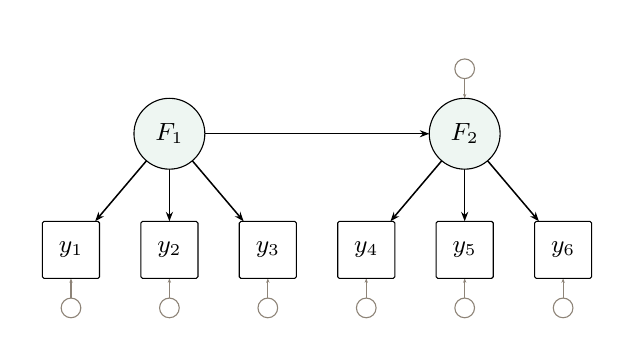
\begin{tikzpicture}[x=1cm, y=1cm,
    obs/.style={draw, rounded corners=0.6pt, minimum size=0.725cm, inner sep=0pt, fill=white, font=\fontsize{9.0}{10}\selectfont},
    lat/.style={draw, circle, minimum size=0.900cm, inner sep=0pt, fill=latfill, font=\fontsize{9.0}{10}\selectfont},
    resid/.style={draw=residc, line width=0.4pt}, residarrow/.style={draw=residc, -{Stealth[length=1.6pt]}, line width=0.4pt},
    path/.style={-{Stealth[length=3.4pt]}, line width=0.55pt},
    cov/.style={{Stealth[length=3.4pt]}-{Stealth[length=3.4pt]}, line width=0.55pt},
    net/.style={draw=netc, line width=1.1pt, line cap=round},
    elabel/.style={font=\scriptsize\itshape, fill=white, inner sep=0.6pt}]
\useasboundingbox (-0.550,-0.053) rectangle (6.800,-3.925);
\draw[resid] (0.000,-3.612) circle (0.125);
\draw[residarrow] (0.000,-3.487) -- (0.000,-3.237);
\draw[resid] (1.250,-3.612) circle (0.125);
\draw[residarrow] (1.250,-3.487) -- (1.250,-3.237);
\draw[resid] (2.500,-3.612) circle (0.125);
\draw[residarrow] (2.500,-3.487) -- (2.500,-3.237);
\draw[resid] (3.750,-3.612) circle (0.125);
\draw[residarrow] (3.750,-3.487) -- (3.750,-3.237);
\draw[resid] (5.000,-3.612) circle (0.125);
\draw[residarrow] (5.000,-3.487) -- (5.000,-3.237);
\draw[resid] (6.250,-3.612) circle (0.125);
\draw[residarrow] (6.250,-3.487) -- (6.250,-3.237);
\draw[resid] (5.000,-0.575) circle (0.125);
\draw[residarrow] (5.000,-0.700) -- (5.000,-0.950);
\draw[path] (0.959,-1.743) -- (0.307,-2.512);
\draw[path] (1.250,-1.850) -- (1.250,-2.512);
\draw[path] (1.541,-1.743) -- (2.193,-2.512);
\draw[path] (4.709,-1.743) -- (4.057,-2.512);
\draw[path] (5.000,-1.850) -- (5.000,-2.512);
\draw[path] (5.291,-1.743) -- (5.943,-2.512);
\draw[path] (1.700,-1.400) -- (4.550,-1.400);
\node[obs] at (0.000,-2.875) {$y_{1}$};
\node[obs] at (1.250,-2.875) {$y_{2}$};
\node[obs] at (2.500,-2.875) {$y_{3}$};
\node[obs] at (3.750,-2.875) {$y_{4}$};
\node[obs] at (5.000,-2.875) {$y_{5}$};
\node[obs] at (6.250,-2.875) {$y_{6}$};
\node[lat] at (1.250,-1.400) {$F_{1}$};
\node[lat] at (5.000,-1.400) {$F_{2}$};
\end{tikzpicture}\\[1pt]{\scriptsize \texttt{F1 =\char`\~{} y1 + y2 + y3; F2 =\char`\~{} y4 + y5 + y6; F2 \char`\~{} F1}}\end{minipage}\hfill
\begin{minipage}[t]{0.49\textwidth}\centering\textbf{\color{bcol}Model B} \;{\small $q_B=13$}\\[2pt]
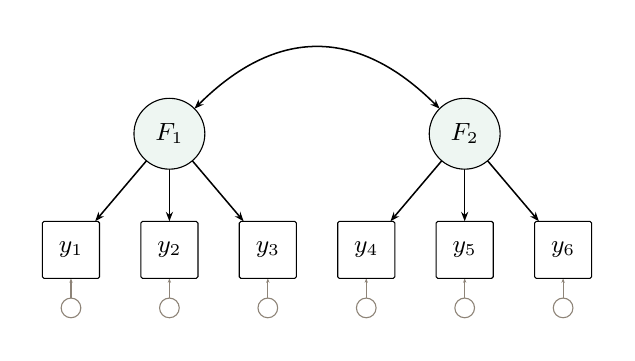
\begin{tikzpicture}[x=1cm, y=1cm,
    obs/.style={draw, rounded corners=0.6pt, minimum size=0.725cm, inner sep=0pt, fill=white, font=\fontsize{9.0}{10}\selectfont},
    lat/.style={draw, circle, minimum size=0.900cm, inner sep=0pt, fill=latfill, font=\fontsize{9.0}{10}\selectfont},
    resid/.style={draw=residc, line width=0.4pt}, residarrow/.style={draw=residc, -{Stealth[length=1.6pt]}, line width=0.4pt},
    path/.style={-{Stealth[length=3.4pt]}, line width=0.55pt},
    cov/.style={{Stealth[length=3.4pt]}-{Stealth[length=3.4pt]}, line width=0.55pt},
    net/.style={draw=netc, line width=1.1pt, line cap=round},
    elabel/.style={font=\scriptsize\itshape, fill=white, inner sep=0.6pt}]
\useasboundingbox (-0.550,-0.053) rectangle (6.800,-3.925);
\draw[resid] (0.000,-3.612) circle (0.125);
\draw[residarrow] (0.000,-3.487) -- (0.000,-3.237);
\draw[resid] (1.250,-3.612) circle (0.125);
\draw[residarrow] (1.250,-3.487) -- (1.250,-3.237);
\draw[resid] (2.500,-3.612) circle (0.125);
\draw[residarrow] (2.500,-3.487) -- (2.500,-3.237);
\draw[resid] (3.750,-3.612) circle (0.125);
\draw[residarrow] (3.750,-3.487) -- (3.750,-3.237);
\draw[resid] (5.000,-3.612) circle (0.125);
\draw[residarrow] (5.000,-3.487) -- (5.000,-3.237);
\draw[resid] (6.250,-3.612) circle (0.125);
\draw[residarrow] (6.250,-3.487) -- (6.250,-3.237);
\draw[path] (0.959,-1.743) -- (0.307,-2.512);
\draw[path] (1.250,-1.850) -- (1.250,-2.512);
\draw[path] (1.541,-1.743) -- (2.193,-2.512);
\draw[path] (4.709,-1.743) -- (4.057,-2.512);
\draw[path] (5.000,-1.850) -- (5.000,-2.512);
\draw[path] (5.291,-1.743) -- (5.943,-2.512);
\draw[cov] (1.568,-1.082) .. controls (2.606,-0.044) and (3.644,-0.044) .. (4.682,-1.082);
\node[obs] at (0.000,-2.875) {$y_{1}$};
\node[obs] at (1.250,-2.875) {$y_{2}$};
\node[obs] at (2.500,-2.875) {$y_{3}$};
\node[obs] at (3.750,-2.875) {$y_{4}$};
\node[obs] at (5.000,-2.875) {$y_{5}$};
\node[obs] at (6.250,-2.875) {$y_{6}$};
\node[lat] at (1.250,-1.400) {$F_{1}$};
\node[lat] at (5.000,-1.400) {$F_{2}$};
\end{tikzpicture}\\[1pt]{\scriptsize \texttt{F1 =\char`\~{} y1 + y2 + y3; F2 =\char`\~{} y4 + y5 + y6; F1 \char`\~{}\char`\~{} F2}}\end{minipage}
\par\bigskip
\noindent\textbf{Claim.} $A \equiv B$: the models are \textbf{equivalent}.\par\smallskip
\noindent\textbf{Proof.} (i) $A\nest B$. The measurement parts are identical; the models differ only in the latent block $(F_1,F_2)$. In $A$, $\Psi=\begin{pmatrix}\psi_{11}&\beta\psi_{11}\\ \beta\psi_{11}&\beta^2\psi_{11}+\zeta\end{pmatrix}$; in $B$, $\Psi$ is free. Both reach every $2\times2$ $\Psi$ with $\psi_{11}\neq0$ ($\beta=\psi_{12}/\psi_{11}$, $\zeta=\psi_{22}-\psi_{12}^2/\psi_{11}$), so by Lemmas~B and G the models are equivalent.\par\smallskip
\noindent(ii) $B\nest A$. Lemma~B: in $B$ the block is free, so $\mathcal M_A\subseteq\mathcal M_B$ trivially; with the map above $\mathcal M_B\subseteq\overline{\mathcal M_A}$.\hfill$\square$\par\medskip
\noindent{\small\textit{In the game:} With only two factors, a regression F1 → F2 and a correlation F1 ↔ F2 both spend one parameter on the single covariance between the factors. The fit is identical.}

\clearpage
\section*{E04 \quad Two saturated models}
\addcontentsline{toc}{subsection}{E04\quad Two saturated models}
\noindent\textit{Level: Easy.} Observed variables: $A, B, C$ ($p=3$, 6 moments).\par\medskip
\noindent\begin{minipage}[t]{0.49\textwidth}\centering\textbf{\color{acol}Model A} \;{\small $q_A=6$}\\[2pt]
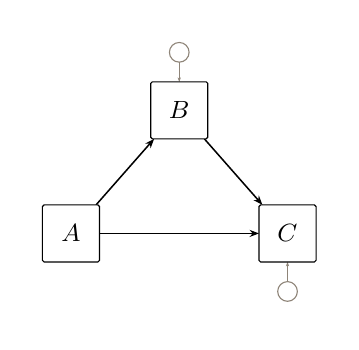
\begin{tikzpicture}[x=1cm, y=1cm,
    obs/.style={draw, rounded corners=0.6pt, minimum size=0.725cm, inner sep=0pt, fill=white, font=\fontsize{9.0}{10}\selectfont},
    lat/.style={draw, circle, minimum size=0.900cm, inner sep=0pt, fill=latfill, font=\fontsize{9.0}{10}\selectfont},
    resid/.style={draw=residc, line width=0.4pt}, residarrow/.style={draw=residc, -{Stealth[length=1.6pt]}, line width=0.4pt},
    path/.style={-{Stealth[length=3.4pt]}, line width=0.55pt},
    cov/.style={{Stealth[length=3.4pt]}-{Stealth[length=3.4pt]}, line width=0.55pt},
    net/.style={draw=netc, line width=1.1pt, line cap=round},
    elabel/.style={font=\scriptsize\itshape, fill=white, inner sep=0.6pt}]
\useasboundingbox (-0.550,1.050) rectangle (3.300,-2.681);
\draw[resid] (1.375,0.737) circle (0.125);
\draw[residarrow] (1.375,0.613) -- (1.375,0.362);
\draw[resid] (2.750,-2.300) circle (0.125);
\draw[residarrow] (2.750,-2.175) -- (2.750,-1.925);
\draw[path] (0.319,-1.200) -- (1.056,-0.362);
\draw[path] (0.362,-1.563) -- (2.388,-1.563);
\draw[path] (1.694,-0.362) -- (2.431,-1.200);
\node[obs] at (0.000,-1.563) {$A$};
\node[obs] at (1.375,0.000) {$B$};
\node[obs] at (2.750,-1.563) {$C$};
\end{tikzpicture}\\[1pt]{\scriptsize \texttt{B \char`\~{} A; C \char`\~{} A + B}}\end{minipage}\hfill
\begin{minipage}[t]{0.49\textwidth}\centering\textbf{\color{bcol}Model B} \;{\small $q_B=6$}\\[2pt]
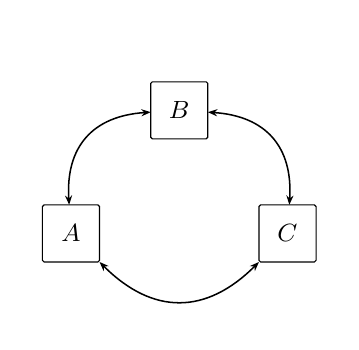
\begin{tikzpicture}[x=1cm, y=1cm,
    obs/.style={draw, rounded corners=0.6pt, minimum size=0.725cm, inner sep=0pt, fill=white, font=\fontsize{9.0}{10}\selectfont},
    lat/.style={draw, circle, minimum size=0.900cm, inner sep=0pt, fill=latfill, font=\fontsize{9.0}{10}\selectfont},
    resid/.style={draw=residc, line width=0.4pt}, residarrow/.style={draw=residc, -{Stealth[length=1.6pt]}, line width=0.4pt},
    path/.style={-{Stealth[length=3.4pt]}, line width=0.55pt},
    cov/.style={{Stealth[length=3.4pt]}-{Stealth[length=3.4pt]}, line width=0.55pt},
    net/.style={draw=netc, line width=1.1pt, line cap=round},
    elabel/.style={font=\scriptsize\itshape, fill=white, inner sep=0.6pt}]
\useasboundingbox (-0.550,1.050) rectangle (3.300,-2.681);
\draw[cov] (-0.023,-1.200) .. controls (-0.070,-0.463) and (0.275,-0.070) .. (1.013,-0.023);
\draw[cov] (0.362,-1.925) .. controls (1.038,-2.600) and (1.713,-2.600) .. (2.388,-1.925);
\draw[cov] (1.738,-0.023) .. controls (2.475,-0.070) and (2.820,-0.463) .. (2.773,-1.200);
\node[obs] at (0.000,-1.563) {$A$};
\node[obs] at (1.375,0.000) {$B$};
\node[obs] at (2.750,-1.563) {$C$};
\end{tikzpicture}\\[1pt]{\scriptsize \texttt{A \char`\~{}\char`\~{} B + C; B \char`\~{}\char`\~{} C}}\end{minipage}
\par\bigskip
\noindent\textbf{Claim.} $A \equiv B$: the models are \textbf{equivalent}.\par\smallskip
\noindent\textbf{Proof.} (i) $A\nest B$. $A$ is a complete recursive path model and $B$ the model with all covariances free; both are saturated (Lemma~B(a)): $\overline{\mathcal M_A}=\overline{\mathcal M_B}=$ all positive definite $3\times3$ matrices.\par\smallskip
\noindent(ii) $B\nest A$. As above.\hfill$\square$\par\medskip
\noindent{\small\textit{In the game:} Both models are saturated: they have as many parameters (6) as there are variances and covariances. Every saturated model reproduces any covariance matrix, so all saturated models are equivalent.}

\clearpage
\section*{E05 \quad One factor with three indicators is saturated}
\addcontentsline{toc}{subsection}{E05\quad One factor with three indicators is saturated}
\noindent\textit{Level: Easy.} Observed variables: $y_{1}, y_{2}, y_{3}$ ($p=3$, 6 moments).\par\medskip
\noindent\begin{minipage}[t]{0.49\textwidth}\centering\textbf{\color{acol}Model A} \;{\small $q_A=6$}\\[2pt]
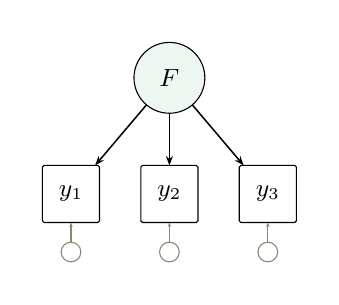
\begin{tikzpicture}[x=1cm, y=1cm,
    obs/.style={draw, rounded corners=0.6pt, minimum size=0.725cm, inner sep=0pt, fill=white, font=\fontsize{9.0}{10}\selectfont},
    lat/.style={draw, circle, minimum size=0.900cm, inner sep=0pt, fill=latfill, font=\fontsize{9.0}{10}\selectfont},
    resid/.style={draw=residc, line width=0.4pt}, residarrow/.style={draw=residc, -{Stealth[length=1.6pt]}, line width=0.4pt},
    path/.style={-{Stealth[length=3.4pt]}, line width=0.55pt},
    cov/.style={{Stealth[length=3.4pt]}-{Stealth[length=3.4pt]}, line width=0.55pt},
    net/.style={draw=netc, line width=1.1pt, line cap=round},
    elabel/.style={font=\scriptsize\itshape, fill=white, inner sep=0.6pt}]
\useasboundingbox (-0.550,-0.763) rectangle (3.050,-3.925);
\draw[resid] (0.000,-3.612) circle (0.125);
\draw[residarrow] (0.000,-3.487) -- (0.000,-3.237);
\draw[resid] (1.250,-3.612) circle (0.125);
\draw[residarrow] (1.250,-3.487) -- (1.250,-3.237);
\draw[resid] (2.500,-3.612) circle (0.125);
\draw[residarrow] (2.500,-3.487) -- (2.500,-3.237);
\draw[path] (0.959,-1.743) -- (0.307,-2.512);
\draw[path] (1.250,-1.850) -- (1.250,-2.512);
\draw[path] (1.541,-1.743) -- (2.193,-2.512);
\node[obs] at (0.000,-2.875) {$y_{1}$};
\node[obs] at (1.250,-2.875) {$y_{2}$};
\node[obs] at (2.500,-2.875) {$y_{3}$};
\node[lat] at (1.250,-1.400) {$F$};
\end{tikzpicture}\\[1pt]{\scriptsize \texttt{F =\char`\~{} y1 + y2 + y3}}\end{minipage}\hfill
\begin{minipage}[t]{0.49\textwidth}\centering\textbf{\color{bcol}Model B} \;{\small $q_B=6$}\\[2pt]
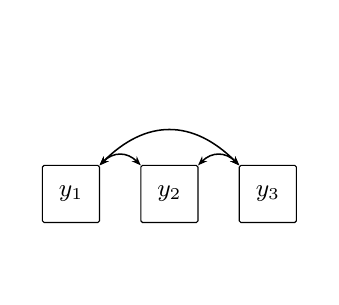
\begin{tikzpicture}[x=1cm, y=1cm,
    obs/.style={draw, rounded corners=0.6pt, minimum size=0.725cm, inner sep=0pt, fill=white, font=\fontsize{9.0}{10}\selectfont},
    lat/.style={draw, circle, minimum size=0.900cm, inner sep=0pt, fill=latfill, font=\fontsize{9.0}{10}\selectfont},
    resid/.style={draw=residc, line width=0.4pt}, residarrow/.style={draw=residc, -{Stealth[length=1.6pt]}, line width=0.4pt},
    path/.style={-{Stealth[length=3.4pt]}, line width=0.55pt},
    cov/.style={{Stealth[length=3.4pt]}-{Stealth[length=3.4pt]}, line width=0.55pt},
    net/.style={draw=netc, line width=1.1pt, line cap=round},
    elabel/.style={font=\scriptsize\itshape, fill=white, inner sep=0.6pt}]
\useasboundingbox (-0.550,-0.763) rectangle (3.050,-3.925);
\draw[cov] (0.362,-2.512) .. controls (0.537,-2.337) and (0.713,-2.337) .. (0.887,-2.512);
\draw[cov] (0.362,-2.512) .. controls (0.954,-1.921) and (1.546,-1.921) .. (2.138,-2.512);
\draw[cov] (1.613,-2.512) .. controls (1.787,-2.337) and (1.963,-2.337) .. (2.138,-2.512);
\node[obs] at (0.000,-2.875) {$y_{1}$};
\node[obs] at (1.250,-2.875) {$y_{2}$};
\node[obs] at (2.500,-2.875) {$y_{3}$};
\end{tikzpicture}\\[1pt]{\scriptsize \texttt{y1 \char`\~{}\char`\~{} y2 + y3; y2 \char`\~{}\char`\~{} y3}}\end{minipage}
\par\bigskip
\noindent\textbf{Claim.} $A \equiv B$: the models are \textbf{equivalent}.\par\smallskip
\noindent\textbf{Proof.} (i) $A\nest B$. $B$ (all covariances free) is saturated, so $A\nest B$.\par\smallskip
\noindent(ii) $B\nest A$. By Lemma~B(a) the one-factor model with three indicators reproduces every $\Sigma\succ0$ with $\sigma_{12}\sigma_{13}\sigma_{23}\neq0$ (a dense set): $\lambda_1=1$, $\psi=\sigma_{12}\sigma_{13}/\sigma_{23}$, $\lambda_2=\sigma_{23}/\sigma_{13}$, $\lambda_3=\sigma_{23}/\sigma_{12}$, $\theta_{ii}=\sigma_{ii}-\lambda_i^2\psi$. ($\psi<0$ when the product of the covariances is negative: a Heywood solution.) Hence $B\nest A$.\hfill$\square$\par\medskip
\noindent{\small\textit{In the game:} A one-factor model with three indicators has 3 loadings and 3 residual variances: 6 parameters for 6 (co)variances. It is just-identified (saturated), like the model with all covariances free.}

\clearpage
\section*{E06 \quad A cross-loading}
\addcontentsline{toc}{subsection}{E06\quad A cross-loading}
\noindent\textit{Level: Easy.} Observed variables: $y_{1}, y_{2}, y_{3}, y_{4}, y_{5}, y_{6}$ ($p=6$, 21 moments).\par\medskip
\noindent\begin{minipage}[t]{0.49\textwidth}\centering\textbf{\color{acol}Model A} \;{\small $q_A=13$}\\[2pt]
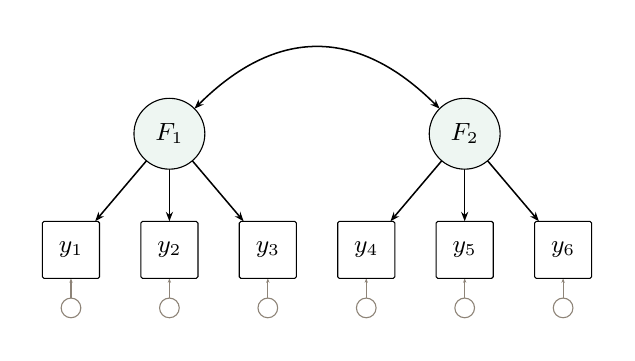
\begin{tikzpicture}[x=1cm, y=1cm,
    obs/.style={draw, rounded corners=0.6pt, minimum size=0.725cm, inner sep=0pt, fill=white, font=\fontsize{9.0}{10}\selectfont},
    lat/.style={draw, circle, minimum size=0.900cm, inner sep=0pt, fill=latfill, font=\fontsize{9.0}{10}\selectfont},
    resid/.style={draw=residc, line width=0.4pt}, residarrow/.style={draw=residc, -{Stealth[length=1.6pt]}, line width=0.4pt},
    path/.style={-{Stealth[length=3.4pt]}, line width=0.55pt},
    cov/.style={{Stealth[length=3.4pt]}-{Stealth[length=3.4pt]}, line width=0.55pt},
    net/.style={draw=netc, line width=1.1pt, line cap=round},
    elabel/.style={font=\scriptsize\itshape, fill=white, inner sep=0.6pt}]
\useasboundingbox (-0.550,-0.053) rectangle (6.800,-3.925);
\draw[resid] (0.000,-3.612) circle (0.125);
\draw[residarrow] (0.000,-3.487) -- (0.000,-3.237);
\draw[resid] (1.250,-3.612) circle (0.125);
\draw[residarrow] (1.250,-3.487) -- (1.250,-3.237);
\draw[resid] (2.500,-3.612) circle (0.125);
\draw[residarrow] (2.500,-3.487) -- (2.500,-3.237);
\draw[resid] (3.750,-3.612) circle (0.125);
\draw[residarrow] (3.750,-3.487) -- (3.750,-3.237);
\draw[resid] (5.000,-3.612) circle (0.125);
\draw[residarrow] (5.000,-3.487) -- (5.000,-3.237);
\draw[resid] (6.250,-3.612) circle (0.125);
\draw[residarrow] (6.250,-3.487) -- (6.250,-3.237);
\draw[path] (0.959,-1.743) -- (0.307,-2.512);
\draw[path] (1.250,-1.850) -- (1.250,-2.512);
\draw[path] (1.541,-1.743) -- (2.193,-2.512);
\draw[path] (4.709,-1.743) -- (4.057,-2.512);
\draw[path] (5.000,-1.850) -- (5.000,-2.512);
\draw[path] (5.291,-1.743) -- (5.943,-2.512);
\draw[cov] (1.568,-1.082) .. controls (2.606,-0.044) and (3.644,-0.044) .. (4.682,-1.082);
\node[obs] at (0.000,-2.875) {$y_{1}$};
\node[obs] at (1.250,-2.875) {$y_{2}$};
\node[obs] at (2.500,-2.875) {$y_{3}$};
\node[obs] at (3.750,-2.875) {$y_{4}$};
\node[obs] at (5.000,-2.875) {$y_{5}$};
\node[obs] at (6.250,-2.875) {$y_{6}$};
\node[lat] at (1.250,-1.400) {$F_{1}$};
\node[lat] at (5.000,-1.400) {$F_{2}$};
\end{tikzpicture}\\[1pt]{\scriptsize \texttt{F1 =\char`\~{} y1 + y2 + y3; F2 =\char`\~{} y4 + y5 + y6; F1 \char`\~{}\char`\~{} F2}}\end{minipage}\hfill
\begin{minipage}[t]{0.49\textwidth}\centering\textbf{\color{bcol}Model B} \;{\small $q_B=14$}\\[2pt]
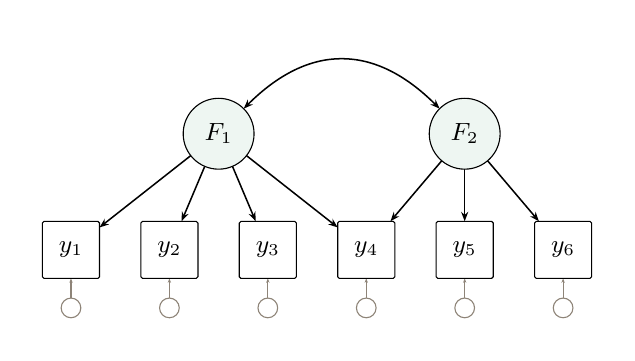
\begin{tikzpicture}[x=1cm, y=1cm,
    obs/.style={draw, rounded corners=0.6pt, minimum size=0.725cm, inner sep=0pt, fill=white, font=\fontsize{9.0}{10}\selectfont},
    lat/.style={draw, circle, minimum size=0.900cm, inner sep=0pt, fill=latfill, font=\fontsize{9.0}{10}\selectfont},
    resid/.style={draw=residc, line width=0.4pt}, residarrow/.style={draw=residc, -{Stealth[length=1.6pt]}, line width=0.4pt},
    path/.style={-{Stealth[length=3.4pt]}, line width=0.55pt},
    cov/.style={{Stealth[length=3.4pt]}-{Stealth[length=3.4pt]}, line width=0.55pt},
    net/.style={draw=netc, line width=1.1pt, line cap=round},
    elabel/.style={font=\scriptsize\itshape, fill=white, inner sep=0.6pt}]
\useasboundingbox (-0.550,-0.053) rectangle (6.800,-3.925);
\draw[resid] (0.000,-3.612) circle (0.125);
\draw[residarrow] (0.000,-3.487) -- (0.000,-3.237);
\draw[resid] (1.250,-3.612) circle (0.125);
\draw[residarrow] (1.250,-3.487) -- (1.250,-3.237);
\draw[resid] (2.500,-3.612) circle (0.125);
\draw[residarrow] (2.500,-3.487) -- (2.500,-3.237);
\draw[resid] (3.750,-3.612) circle (0.125);
\draw[residarrow] (3.750,-3.487) -- (3.750,-3.237);
\draw[resid] (5.000,-3.612) circle (0.125);
\draw[residarrow] (5.000,-3.487) -- (5.000,-3.237);
\draw[resid] (6.250,-3.612) circle (0.125);
\draw[residarrow] (6.250,-3.487) -- (6.250,-3.237);
\draw[path] (1.521,-1.678) -- (0.362,-2.590);
\draw[path] (1.699,-1.814) -- (1.404,-2.512);
\draw[path] (2.051,-1.814) -- (2.346,-2.512);
\draw[path] (2.229,-1.678) -- (3.388,-2.590);
\draw[path] (4.709,-1.743) -- (4.057,-2.512);
\draw[path] (5.000,-1.850) -- (5.000,-2.512);
\draw[path] (5.291,-1.743) -- (5.943,-2.512);
\draw[cov] (2.193,-1.082) .. controls (3.023,-0.252) and (3.852,-0.252) .. (4.682,-1.082);
\node[obs] at (0.000,-2.875) {$y_{1}$};
\node[obs] at (1.250,-2.875) {$y_{2}$};
\node[obs] at (2.500,-2.875) {$y_{3}$};
\node[obs] at (3.750,-2.875) {$y_{4}$};
\node[obs] at (5.000,-2.875) {$y_{5}$};
\node[obs] at (6.250,-2.875) {$y_{6}$};
\node[lat] at (1.875,-1.400) {$F_{1}$};
\node[lat] at (5.000,-1.400) {$F_{2}$};
\end{tikzpicture}\\[1pt]{\scriptsize \texttt{F1 =\char`\~{} y1 + y2 + y3 + y4; F2 =\char`\~{} y4 + y5 + y6; F1 \char`\~{}\char`\~{} F2}}\end{minipage}
\par\bigskip
\noindent\textbf{Claim.} $A \nest B$, $B \nnest A$: \textbf{A is nested in B} (strictly).\par\smallskip
\noindent\textbf{Proof.} (i) $A\nest B$. Fix the cross-loading of $y_4$ on $F_1$ in $B$ to $0$ (Lemma~R).\par\smallskip
\noindent(ii) $B\nnest A$ by Lemma~D: the Jacobian of model $B$ has rank 14 at the rational point listed in Appendix~B, while model $A$ has only $q_A=13$ free parameters.\hfill$\square$\par\medskip
\noindent{\small\textit{In the game:} B is A plus one cross-loading (F1 → y4). Fix that loading to zero and you get A back, so A is nested in B.}

\clearpage
\section*{E07 \quad One factor versus two}
\addcontentsline{toc}{subsection}{E07\quad One factor versus two}
\noindent\textit{Level: Easy.} Observed variables: $y_{1}, y_{2}, y_{3}, y_{4}, y_{5}, y_{6}$ ($p=6$, 21 moments).\par\medskip
\noindent\begin{minipage}[t]{0.49\textwidth}\centering\textbf{\color{acol}Model A} \;{\small $q_A=12$}\\[2pt]
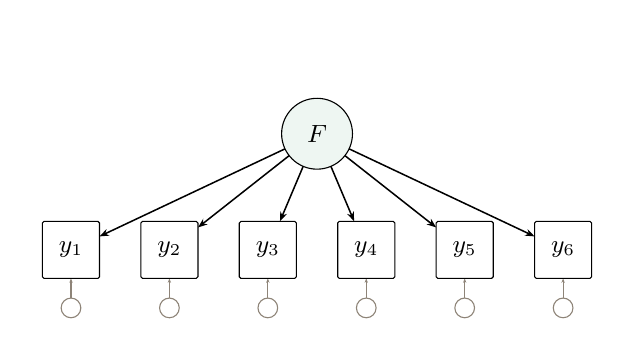
\begin{tikzpicture}[x=1cm, y=1cm,
    obs/.style={draw, rounded corners=0.6pt, minimum size=0.725cm, inner sep=0pt, fill=white, font=\fontsize{9.0}{10}\selectfont},
    lat/.style={draw, circle, minimum size=0.900cm, inner sep=0pt, fill=latfill, font=\fontsize{9.0}{10}\selectfont},
    resid/.style={draw=residc, line width=0.4pt}, residarrow/.style={draw=residc, -{Stealth[length=1.6pt]}, line width=0.4pt},
    path/.style={-{Stealth[length=3.4pt]}, line width=0.55pt},
    cov/.style={{Stealth[length=3.4pt]}-{Stealth[length=3.4pt]}, line width=0.55pt},
    net/.style={draw=netc, line width=1.1pt, line cap=round},
    elabel/.style={font=\scriptsize\itshape, fill=white, inner sep=0.6pt}]
\useasboundingbox (-0.550,-0.053) rectangle (6.800,-3.925);
\draw[resid] (0.000,-3.612) circle (0.125);
\draw[residarrow] (0.000,-3.487) -- (0.000,-3.237);
\draw[resid] (1.250,-3.612) circle (0.125);
\draw[residarrow] (1.250,-3.487) -- (1.250,-3.237);
\draw[resid] (2.500,-3.612) circle (0.125);
\draw[residarrow] (2.500,-3.487) -- (2.500,-3.237);
\draw[resid] (3.750,-3.612) circle (0.125);
\draw[residarrow] (3.750,-3.487) -- (3.750,-3.237);
\draw[resid] (5.000,-3.612) circle (0.125);
\draw[residarrow] (5.000,-3.487) -- (5.000,-3.237);
\draw[resid] (6.250,-3.612) circle (0.125);
\draw[residarrow] (6.250,-3.487) -- (6.250,-3.237);
\draw[path] (2.718,-1.592) -- (0.362,-2.704);
\draw[path] (2.771,-1.678) -- (1.613,-2.590);
\draw[path] (2.949,-1.814) -- (2.654,-2.512);
\draw[path] (3.301,-1.814) -- (3.596,-2.512);
\draw[path] (3.479,-1.678) -- (4.638,-2.590);
\draw[path] (3.532,-1.592) -- (5.888,-2.704);
\node[obs] at (0.000,-2.875) {$y_{1}$};
\node[obs] at (1.250,-2.875) {$y_{2}$};
\node[obs] at (2.500,-2.875) {$y_{3}$};
\node[obs] at (3.750,-2.875) {$y_{4}$};
\node[obs] at (5.000,-2.875) {$y_{5}$};
\node[obs] at (6.250,-2.875) {$y_{6}$};
\node[lat] at (3.125,-1.400) {$F$};
\end{tikzpicture}\\[1pt]{\scriptsize \texttt{F =\char`\~{} y1 + y2 + y3 + y4 + y5 + y6}}\end{minipage}\hfill
\begin{minipage}[t]{0.49\textwidth}\centering\textbf{\color{bcol}Model B} \;{\small $q_B=13$}\\[2pt]
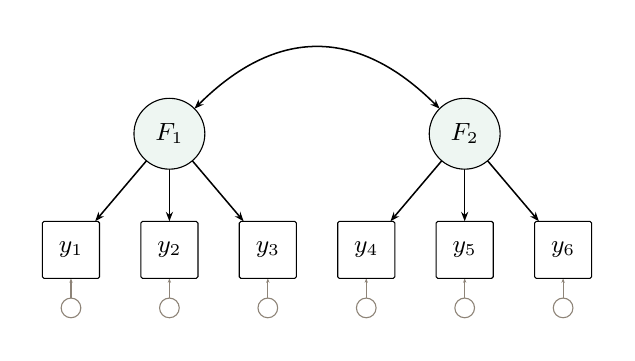
\begin{tikzpicture}[x=1cm, y=1cm,
    obs/.style={draw, rounded corners=0.6pt, minimum size=0.725cm, inner sep=0pt, fill=white, font=\fontsize{9.0}{10}\selectfont},
    lat/.style={draw, circle, minimum size=0.900cm, inner sep=0pt, fill=latfill, font=\fontsize{9.0}{10}\selectfont},
    resid/.style={draw=residc, line width=0.4pt}, residarrow/.style={draw=residc, -{Stealth[length=1.6pt]}, line width=0.4pt},
    path/.style={-{Stealth[length=3.4pt]}, line width=0.55pt},
    cov/.style={{Stealth[length=3.4pt]}-{Stealth[length=3.4pt]}, line width=0.55pt},
    net/.style={draw=netc, line width=1.1pt, line cap=round},
    elabel/.style={font=\scriptsize\itshape, fill=white, inner sep=0.6pt}]
\useasboundingbox (-0.550,-0.053) rectangle (6.800,-3.925);
\draw[resid] (0.000,-3.612) circle (0.125);
\draw[residarrow] (0.000,-3.487) -- (0.000,-3.237);
\draw[resid] (1.250,-3.612) circle (0.125);
\draw[residarrow] (1.250,-3.487) -- (1.250,-3.237);
\draw[resid] (2.500,-3.612) circle (0.125);
\draw[residarrow] (2.500,-3.487) -- (2.500,-3.237);
\draw[resid] (3.750,-3.612) circle (0.125);
\draw[residarrow] (3.750,-3.487) -- (3.750,-3.237);
\draw[resid] (5.000,-3.612) circle (0.125);
\draw[residarrow] (5.000,-3.487) -- (5.000,-3.237);
\draw[resid] (6.250,-3.612) circle (0.125);
\draw[residarrow] (6.250,-3.487) -- (6.250,-3.237);
\draw[path] (0.959,-1.743) -- (0.307,-2.512);
\draw[path] (1.250,-1.850) -- (1.250,-2.512);
\draw[path] (1.541,-1.743) -- (2.193,-2.512);
\draw[path] (4.709,-1.743) -- (4.057,-2.512);
\draw[path] (5.000,-1.850) -- (5.000,-2.512);
\draw[path] (5.291,-1.743) -- (5.943,-2.512);
\draw[cov] (1.568,-1.082) .. controls (2.606,-0.044) and (3.644,-0.044) .. (4.682,-1.082);
\node[obs] at (0.000,-2.875) {$y_{1}$};
\node[obs] at (1.250,-2.875) {$y_{2}$};
\node[obs] at (2.500,-2.875) {$y_{3}$};
\node[obs] at (3.750,-2.875) {$y_{4}$};
\node[obs] at (5.000,-2.875) {$y_{5}$};
\node[obs] at (6.250,-2.875) {$y_{6}$};
\node[lat] at (1.250,-1.400) {$F_{1}$};
\node[lat] at (5.000,-1.400) {$F_{2}$};
\end{tikzpicture}\\[1pt]{\scriptsize \texttt{F1 =\char`\~{} y1 + y2 + y3; F2 =\char`\~{} y4 + y5 + y6; F1 \char`\~{}\char`\~{} F2}}\end{minipage}
\par\bigskip
\noindent\textbf{Claim.} $A \nest B$, $B \nnest A$: \textbf{A is nested in B} (strictly).\par\smallskip
\noindent\textbf{Proof.} (i) $A\nest B$. Lemma~M: in $B$ take $\psi_{11}=\psi_{22}=\psi_{12}$; then $F_1$ and $F_2$ act as one factor and $B$ reproduces $A$.\par\smallskip
\noindent(ii) $B\nnest A$ by Lemma~D: the Jacobian of model $B$ has rank 13 at the rational point listed in Appendix~B, while model $A$ has only $q_A=12$ free parameters.\hfill$\square$\par\medskip
\noindent{\small\textit{In the game:} A one-factor model is a two-factor model whose factors correlate perfectly (r = 1). So the one-factor model is nested in the two-factor model.}

\clearpage
\section*{E08 \quad Adding a direct effect}
\addcontentsline{toc}{subsection}{E08\quad Adding a direct effect}
\noindent\textit{Level: Easy.} Observed variables: $A, B, C$ ($p=3$, 6 moments).\par\medskip
\noindent\begin{minipage}[t]{0.49\textwidth}\centering\textbf{\color{acol}Model A} \;{\small $q_A=5$}\\[2pt]
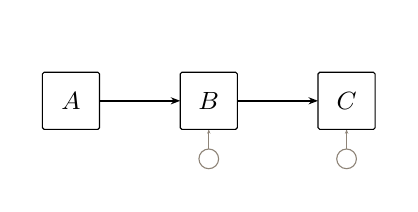
\begin{tikzpicture}[x=1cm, y=1cm,
    obs/.style={draw, rounded corners=0.6pt, minimum size=0.725cm, inner sep=0pt, fill=white, font=\fontsize{9.0}{10}\selectfont},
    lat/.style={draw, circle, minimum size=0.900cm, inner sep=0pt, fill=latfill, font=\fontsize{9.0}{10}\selectfont},
    resid/.style={draw=residc, line width=0.4pt}, residarrow/.style={draw=residc, -{Stealth[length=1.6pt]}, line width=0.4pt},
    path/.style={-{Stealth[length=3.4pt]}, line width=0.55pt},
    cov/.style={{Stealth[length=3.4pt]}-{Stealth[length=3.4pt]}, line width=0.55pt},
    net/.style={draw=netc, line width=1.1pt, line cap=round},
    elabel/.style={font=\scriptsize\itshape, fill=white, inner sep=0.6pt}]
\useasboundingbox (-0.550,0.929) rectangle (4.050,-1.050);
\draw[resid] (1.750,-0.737) circle (0.125);
\draw[residarrow] (1.750,-0.613) -- (1.750,-0.362);
\draw[resid] (3.500,-0.737) circle (0.125);
\draw[residarrow] (3.500,-0.613) -- (3.500,-0.362);
\draw[path] (0.362,0.000) -- (1.387,0.000);
\draw[path] (2.112,0.000) -- (3.137,0.000);
\node[obs] at (0.000,0.000) {$A$};
\node[obs] at (1.750,0.000) {$B$};
\node[obs] at (3.500,0.000) {$C$};
\end{tikzpicture}\\[1pt]{\scriptsize \texttt{B \char`\~{} A; C \char`\~{} B}}\end{minipage}\hfill
\begin{minipage}[t]{0.49\textwidth}\centering\textbf{\color{bcol}Model B} \;{\small $q_B=6$}\\[2pt]
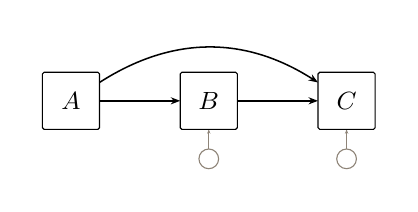
\begin{tikzpicture}[x=1cm, y=1cm,
    obs/.style={draw, rounded corners=0.6pt, minimum size=0.725cm, inner sep=0pt, fill=white, font=\fontsize{9.0}{10}\selectfont},
    lat/.style={draw, circle, minimum size=0.900cm, inner sep=0pt, fill=latfill, font=\fontsize{9.0}{10}\selectfont},
    resid/.style={draw=residc, line width=0.4pt}, residarrow/.style={draw=residc, -{Stealth[length=1.6pt]}, line width=0.4pt},
    path/.style={-{Stealth[length=3.4pt]}, line width=0.55pt},
    cov/.style={{Stealth[length=3.4pt]}-{Stealth[length=3.4pt]}, line width=0.55pt},
    net/.style={draw=netc, line width=1.1pt, line cap=round},
    elabel/.style={font=\scriptsize\itshape, fill=white, inner sep=0.6pt}]
\useasboundingbox (-0.550,0.929) rectangle (4.050,-1.050);
\draw[resid] (1.750,-0.737) circle (0.125);
\draw[residarrow] (1.750,-0.613) -- (1.750,-0.362);
\draw[resid] (3.500,-0.737) circle (0.125);
\draw[residarrow] (3.500,-0.613) -- (3.500,-0.362);
\draw[path] (0.362,0.000) -- (1.387,0.000);
\draw[path] (0.362,0.233) .. controls (1.287,0.828) and (2.212,0.828) .. (3.137,0.233);
\draw[path] (2.112,0.000) -- (3.137,0.000);
\node[obs] at (0.000,0.000) {$A$};
\node[obs] at (1.750,0.000) {$B$};
\node[obs] at (3.500,0.000) {$C$};
\end{tikzpicture}\\[1pt]{\scriptsize \texttt{B \char`\~{} A; C \char`\~{} A + B}}\end{minipage}
\par\bigskip
\noindent\textbf{Claim.} $A \nest B$, $B \nnest A$: \textbf{A is nested in B} (strictly).\par\smallskip
\noindent\textbf{Proof.} (i) $A\nest B$. Fix $\beta_{CA}=0$ in $B$ (Lemma~R).\par\smallskip
\noindent(ii) $B\nnest A$ by Lemma~D: the Jacobian of model $B$ has rank 6 at the rational point listed in Appendix~B, while model $A$ has only $q_A=5$ free parameters.\hfill$\square$\par\medskip
\noindent{\small\textit{In the game:} B adds the direct effect A → C (and is saturated). Setting that effect to zero gives A: A is nested in B.}

\clearpage
\section*{E09 \quad A latent chain versus correlated factors}
\addcontentsline{toc}{subsection}{E09\quad A latent chain versus correlated factors}
\noindent\textit{Level: Easy.} Observed variables: $y_{1}, y_{2}, y_{3}, y_{4}, y_{5}, y_{6}$ ($p=6$, 21 moments).\par\medskip
\noindent\begin{minipage}[t]{0.49\textwidth}\centering\textbf{\color{acol}Model A} \;{\small $q_A=14$}\\[2pt]
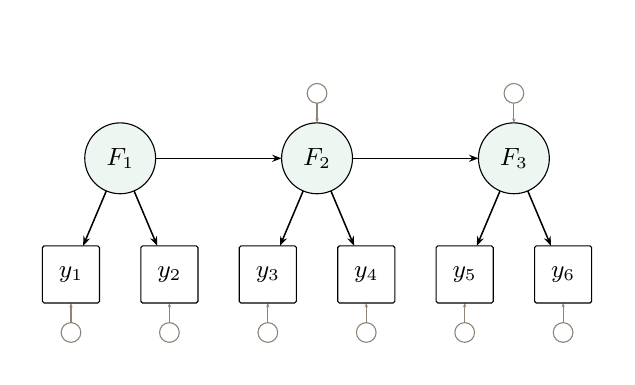
\begin{tikzpicture}[x=1cm, y=1cm,
    obs/.style={draw, rounded corners=0.6pt, minimum size=0.725cm, inner sep=0pt, fill=white, font=\fontsize{9.0}{10}\selectfont},
    lat/.style={draw, circle, minimum size=0.900cm, inner sep=0pt, fill=latfill, font=\fontsize{9.0}{10}\selectfont},
    resid/.style={draw=residc, line width=0.4pt}, residarrow/.style={draw=residc, -{Stealth[length=1.6pt]}, line width=0.4pt},
    path/.style={-{Stealth[length=3.4pt]}, line width=0.55pt},
    cov/.style={{Stealth[length=3.4pt]}-{Stealth[length=3.4pt]}, line width=0.55pt},
    net/.style={draw=netc, line width=1.1pt, line cap=round},
    elabel/.style={font=\scriptsize\itshape, fill=white, inner sep=0.6pt}]
\useasboundingbox (-0.550,0.259) rectangle (6.800,-3.925);
\draw[resid] (0.000,-3.612) circle (0.125);
\draw[residarrow] (0.000,-3.487) -- (0.000,-3.237);
\draw[resid] (1.250,-3.612) circle (0.125);
\draw[residarrow] (1.250,-3.487) -- (1.250,-3.237);
\draw[resid] (2.500,-3.612) circle (0.125);
\draw[residarrow] (2.500,-3.487) -- (2.500,-3.237);
\draw[resid] (3.750,-3.612) circle (0.125);
\draw[residarrow] (3.750,-3.487) -- (3.750,-3.237);
\draw[resid] (5.000,-3.612) circle (0.125);
\draw[residarrow] (5.000,-3.487) -- (5.000,-3.237);
\draw[resid] (6.250,-3.612) circle (0.125);
\draw[residarrow] (6.250,-3.487) -- (6.250,-3.237);
\draw[resid] (3.125,-0.575) circle (0.125);
\draw[residarrow] (3.125,-0.700) -- (3.125,-0.950);
\draw[resid] (5.625,-0.575) circle (0.125);
\draw[residarrow] (5.625,-0.700) -- (5.625,-0.950);
\draw[path] (0.449,-1.814) -- (0.154,-2.512);
\draw[path] (0.801,-1.814) -- (1.096,-2.512);
\draw[path] (2.949,-1.814) -- (2.654,-2.512);
\draw[path] (3.301,-1.814) -- (3.596,-2.512);
\draw[path] (5.449,-1.814) -- (5.154,-2.512);
\draw[path] (5.801,-1.814) -- (6.096,-2.512);
\draw[path] (1.075,-1.400) -- (2.675,-1.400);
\draw[path] (3.575,-1.400) -- (5.175,-1.400);
\node[obs] at (0.000,-2.875) {$y_{1}$};
\node[obs] at (1.250,-2.875) {$y_{2}$};
\node[obs] at (2.500,-2.875) {$y_{3}$};
\node[obs] at (3.750,-2.875) {$y_{4}$};
\node[obs] at (5.000,-2.875) {$y_{5}$};
\node[obs] at (6.250,-2.875) {$y_{6}$};
\node[lat] at (0.625,-1.400) {$F_{1}$};
\node[lat] at (3.125,-1.400) {$F_{2}$};
\node[lat] at (5.625,-1.400) {$F_{3}$};
\end{tikzpicture}\\[1pt]{\scriptsize \texttt{F1 =\char`\~{} y1 + y2; F2 =\char`\~{} y3 + y4; F3 =\char`\~{} y5 + y6; F2 \char`\~{} F1; F3 \char`\~{} F2}}\end{minipage}\hfill
\begin{minipage}[t]{0.49\textwidth}\centering\textbf{\color{bcol}Model B} \;{\small $q_B=15$}\\[2pt]
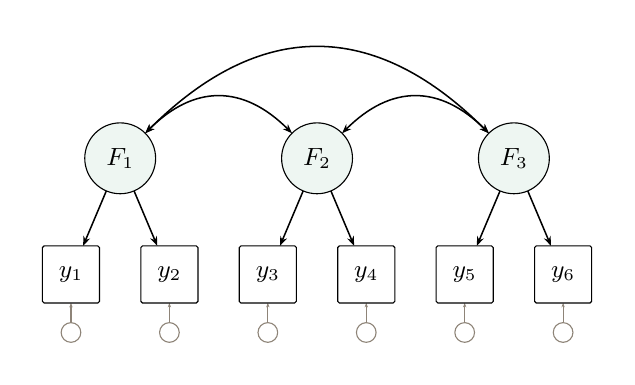
\begin{tikzpicture}[x=1cm, y=1cm,
    obs/.style={draw, rounded corners=0.6pt, minimum size=0.725cm, inner sep=0pt, fill=white, font=\fontsize{9.0}{10}\selectfont},
    lat/.style={draw, circle, minimum size=0.900cm, inner sep=0pt, fill=latfill, font=\fontsize{9.0}{10}\selectfont},
    resid/.style={draw=residc, line width=0.4pt}, residarrow/.style={draw=residc, -{Stealth[length=1.6pt]}, line width=0.4pt},
    path/.style={-{Stealth[length=3.4pt]}, line width=0.55pt},
    cov/.style={{Stealth[length=3.4pt]}-{Stealth[length=3.4pt]}, line width=0.55pt},
    net/.style={draw=netc, line width=1.1pt, line cap=round},
    elabel/.style={font=\scriptsize\itshape, fill=white, inner sep=0.6pt}]
\useasboundingbox (-0.550,0.259) rectangle (6.800,-3.925);
\draw[resid] (0.000,-3.612) circle (0.125);
\draw[residarrow] (0.000,-3.487) -- (0.000,-3.237);
\draw[resid] (1.250,-3.612) circle (0.125);
\draw[residarrow] (1.250,-3.487) -- (1.250,-3.237);
\draw[resid] (2.500,-3.612) circle (0.125);
\draw[residarrow] (2.500,-3.487) -- (2.500,-3.237);
\draw[resid] (3.750,-3.612) circle (0.125);
\draw[residarrow] (3.750,-3.487) -- (3.750,-3.237);
\draw[resid] (5.000,-3.612) circle (0.125);
\draw[residarrow] (5.000,-3.487) -- (5.000,-3.237);
\draw[resid] (6.250,-3.612) circle (0.125);
\draw[residarrow] (6.250,-3.487) -- (6.250,-3.237);
\draw[path] (0.449,-1.814) -- (0.154,-2.512);
\draw[path] (0.801,-1.814) -- (1.096,-2.512);
\draw[path] (2.949,-1.814) -- (2.654,-2.512);
\draw[path] (3.301,-1.814) -- (3.596,-2.512);
\draw[path] (5.449,-1.814) -- (5.154,-2.512);
\draw[path] (5.801,-1.814) -- (6.096,-2.512);
\draw[cov] (0.943,-1.082) .. controls (1.564,-0.461) and (2.186,-0.461) .. (2.807,-1.082);
\draw[cov] (0.943,-1.082) .. controls (2.398,0.373) and (3.852,0.373) .. (5.307,-1.082);
\draw[cov] (3.443,-1.082) .. controls (4.064,-0.461) and (4.686,-0.461) .. (5.307,-1.082);
\node[obs] at (0.000,-2.875) {$y_{1}$};
\node[obs] at (1.250,-2.875) {$y_{2}$};
\node[obs] at (2.500,-2.875) {$y_{3}$};
\node[obs] at (3.750,-2.875) {$y_{4}$};
\node[obs] at (5.000,-2.875) {$y_{5}$};
\node[obs] at (6.250,-2.875) {$y_{6}$};
\node[lat] at (0.625,-1.400) {$F_{1}$};
\node[lat] at (3.125,-1.400) {$F_{2}$};
\node[lat] at (5.625,-1.400) {$F_{3}$};
\end{tikzpicture}\\[1pt]{\scriptsize \texttt{F1 =\char`\~{} y1 + y2; F2 =\char`\~{} y3 + y4; F3 =\char`\~{} y5 + y6; F1 \char`\~{}\char`\~{} F2 + F3; F2 \char`\~{}\char`\~{} F3}}\end{minipage}
\par\bigskip
\noindent\textbf{Claim.} $A \nest B$, $B \nnest A$: \textbf{A is nested in B} (strictly).\par\smallskip
\noindent\textbf{Proof.} (i) $A\nest B$. Same measurement part; in $B$ the latent covariance matrix $\Psi$ is free (a saturated latent block), and the chain in $A$ produces one particular $\Psi$. By Lemma~B(b), $A\nest B$.\par\smallskip
\noindent(ii) $B\nnest A$ by Lemma~D: the Jacobian of model $B$ has rank 15 at the rational point listed in Appendix~B, while model $A$ has only $q_A=14$ free parameters.\hfill$\square$\par\medskip
\noindent{\small\textit{In the game:} B leaves the three factor covariances free (a saturated latent block). The chain F1 → F2 → F3 restricts them (no direct F1–F3 link), so A is nested in B.}

\clearpage
\section*{E10 \quad Orthogonal versus correlated factors}
\addcontentsline{toc}{subsection}{E10\quad Orthogonal versus correlated factors}
\noindent\textit{Level: Easy.} Observed variables: $y_{1}, y_{2}, y_{3}, y_{4}, y_{5}, y_{6}$ ($p=6$, 21 moments).\par\medskip
\noindent\begin{minipage}[t]{0.49\textwidth}\centering\textbf{\color{acol}Model A} \;{\small $q_A=12$}\\[2pt]
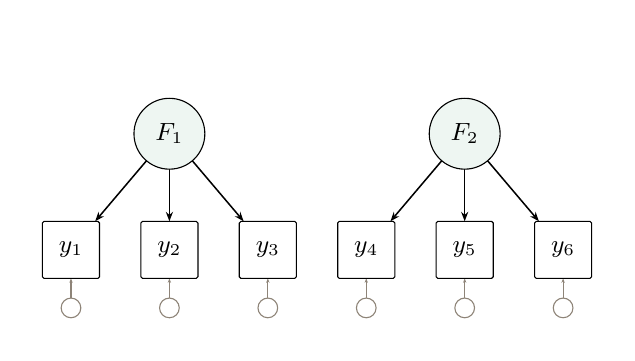
\begin{tikzpicture}[x=1cm, y=1cm,
    obs/.style={draw, rounded corners=0.6pt, minimum size=0.725cm, inner sep=0pt, fill=white, font=\fontsize{9.0}{10}\selectfont},
    lat/.style={draw, circle, minimum size=0.900cm, inner sep=0pt, fill=latfill, font=\fontsize{9.0}{10}\selectfont},
    resid/.style={draw=residc, line width=0.4pt}, residarrow/.style={draw=residc, -{Stealth[length=1.6pt]}, line width=0.4pt},
    path/.style={-{Stealth[length=3.4pt]}, line width=0.55pt},
    cov/.style={{Stealth[length=3.4pt]}-{Stealth[length=3.4pt]}, line width=0.55pt},
    net/.style={draw=netc, line width=1.1pt, line cap=round},
    elabel/.style={font=\scriptsize\itshape, fill=white, inner sep=0.6pt}]
\useasboundingbox (-0.550,-0.053) rectangle (6.800,-3.925);
\draw[resid] (0.000,-3.612) circle (0.125);
\draw[residarrow] (0.000,-3.487) -- (0.000,-3.237);
\draw[resid] (1.250,-3.612) circle (0.125);
\draw[residarrow] (1.250,-3.487) -- (1.250,-3.237);
\draw[resid] (2.500,-3.612) circle (0.125);
\draw[residarrow] (2.500,-3.487) -- (2.500,-3.237);
\draw[resid] (3.750,-3.612) circle (0.125);
\draw[residarrow] (3.750,-3.487) -- (3.750,-3.237);
\draw[resid] (5.000,-3.612) circle (0.125);
\draw[residarrow] (5.000,-3.487) -- (5.000,-3.237);
\draw[resid] (6.250,-3.612) circle (0.125);
\draw[residarrow] (6.250,-3.487) -- (6.250,-3.237);
\draw[path] (0.959,-1.743) -- (0.307,-2.512);
\draw[path] (1.250,-1.850) -- (1.250,-2.512);
\draw[path] (1.541,-1.743) -- (2.193,-2.512);
\draw[path] (4.709,-1.743) -- (4.057,-2.512);
\draw[path] (5.000,-1.850) -- (5.000,-2.512);
\draw[path] (5.291,-1.743) -- (5.943,-2.512);
\node[obs] at (0.000,-2.875) {$y_{1}$};
\node[obs] at (1.250,-2.875) {$y_{2}$};
\node[obs] at (2.500,-2.875) {$y_{3}$};
\node[obs] at (3.750,-2.875) {$y_{4}$};
\node[obs] at (5.000,-2.875) {$y_{5}$};
\node[obs] at (6.250,-2.875) {$y_{6}$};
\node[lat] at (1.250,-1.400) {$F_{1}$};
\node[lat] at (5.000,-1.400) {$F_{2}$};
\end{tikzpicture}\\[1pt]{\scriptsize \texttt{F1 =\char`\~{} y1 + y2 + y3; F2 =\char`\~{} y4 + y5 + y6}}\end{minipage}\hfill
\begin{minipage}[t]{0.49\textwidth}\centering\textbf{\color{bcol}Model B} \;{\small $q_B=13$}\\[2pt]
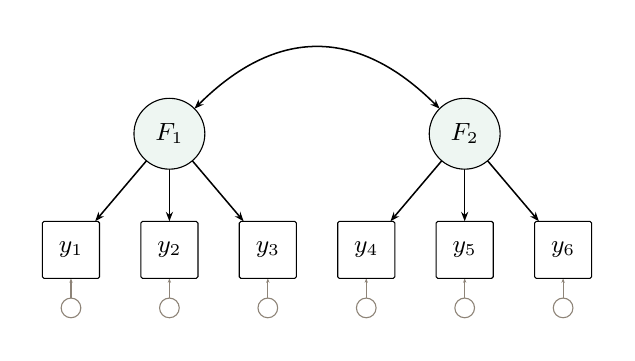
\begin{tikzpicture}[x=1cm, y=1cm,
    obs/.style={draw, rounded corners=0.6pt, minimum size=0.725cm, inner sep=0pt, fill=white, font=\fontsize{9.0}{10}\selectfont},
    lat/.style={draw, circle, minimum size=0.900cm, inner sep=0pt, fill=latfill, font=\fontsize{9.0}{10}\selectfont},
    resid/.style={draw=residc, line width=0.4pt}, residarrow/.style={draw=residc, -{Stealth[length=1.6pt]}, line width=0.4pt},
    path/.style={-{Stealth[length=3.4pt]}, line width=0.55pt},
    cov/.style={{Stealth[length=3.4pt]}-{Stealth[length=3.4pt]}, line width=0.55pt},
    net/.style={draw=netc, line width=1.1pt, line cap=round},
    elabel/.style={font=\scriptsize\itshape, fill=white, inner sep=0.6pt}]
\useasboundingbox (-0.550,-0.053) rectangle (6.800,-3.925);
\draw[resid] (0.000,-3.612) circle (0.125);
\draw[residarrow] (0.000,-3.487) -- (0.000,-3.237);
\draw[resid] (1.250,-3.612) circle (0.125);
\draw[residarrow] (1.250,-3.487) -- (1.250,-3.237);
\draw[resid] (2.500,-3.612) circle (0.125);
\draw[residarrow] (2.500,-3.487) -- (2.500,-3.237);
\draw[resid] (3.750,-3.612) circle (0.125);
\draw[residarrow] (3.750,-3.487) -- (3.750,-3.237);
\draw[resid] (5.000,-3.612) circle (0.125);
\draw[residarrow] (5.000,-3.487) -- (5.000,-3.237);
\draw[resid] (6.250,-3.612) circle (0.125);
\draw[residarrow] (6.250,-3.487) -- (6.250,-3.237);
\draw[path] (0.959,-1.743) -- (0.307,-2.512);
\draw[path] (1.250,-1.850) -- (1.250,-2.512);
\draw[path] (1.541,-1.743) -- (2.193,-2.512);
\draw[path] (4.709,-1.743) -- (4.057,-2.512);
\draw[path] (5.000,-1.850) -- (5.000,-2.512);
\draw[path] (5.291,-1.743) -- (5.943,-2.512);
\draw[cov] (1.568,-1.082) .. controls (2.606,-0.044) and (3.644,-0.044) .. (4.682,-1.082);
\node[obs] at (0.000,-2.875) {$y_{1}$};
\node[obs] at (1.250,-2.875) {$y_{2}$};
\node[obs] at (2.500,-2.875) {$y_{3}$};
\node[obs] at (3.750,-2.875) {$y_{4}$};
\node[obs] at (5.000,-2.875) {$y_{5}$};
\node[obs] at (6.250,-2.875) {$y_{6}$};
\node[lat] at (1.250,-1.400) {$F_{1}$};
\node[lat] at (5.000,-1.400) {$F_{2}$};
\end{tikzpicture}\\[1pt]{\scriptsize \texttt{F1 =\char`\~{} y1 + y2 + y3; F2 =\char`\~{} y4 + y5 + y6; F1 \char`\~{}\char`\~{} F2}}\end{minipage}
\par\bigskip
\noindent\textbf{Claim.} $A \nest B$, $B \nnest A$: \textbf{A is nested in B} (strictly).\par\smallskip
\noindent\textbf{Proof.} (i) $A\nest B$. Fix $\psi_{12}=0$ in $B$ (Lemma~R).\par\smallskip
\noindent(ii) $B\nnest A$ by Lemma~D: the Jacobian of model $B$ has rank 13 at the rational point listed in Appendix~B, while model $A$ has only $q_A=12$ free parameters.\hfill$\square$\par\medskip
\noindent{\small\textit{In the game:} Orthogonal factors are correlated factors with the correlation fixed to zero: A is nested in B.}

\clearpage
\section*{E11 \quad One residual covariance more}
\addcontentsline{toc}{subsection}{E11\quad One residual covariance more}
\noindent\textit{Level: Easy.} Observed variables: $y_{1}, y_{2}, y_{3}, y_{4}, y_{5}, y_{6}$ ($p=6$, 21 moments).\par\medskip
\noindent\begin{minipage}[t]{0.49\textwidth}\centering\textbf{\color{acol}Model A} \;{\small $q_A=14$}\\[2pt]
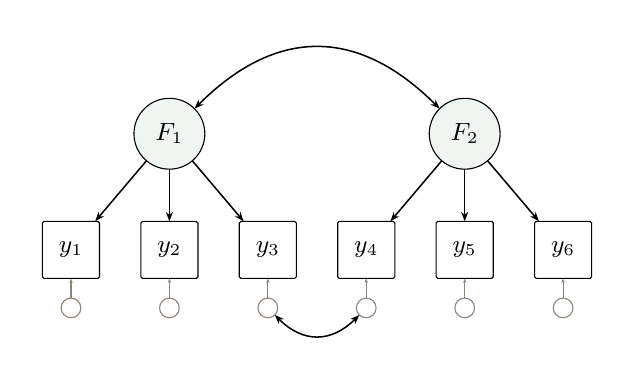
\begin{tikzpicture}[x=1cm, y=1cm,
    obs/.style={draw, rounded corners=0.6pt, minimum size=0.725cm, inner sep=0pt, fill=white, font=\fontsize{9.0}{10}\selectfont},
    lat/.style={draw, circle, minimum size=0.900cm, inner sep=0pt, fill=latfill, font=\fontsize{9.0}{10}\selectfont},
    resid/.style={draw=residc, line width=0.4pt}, residarrow/.style={draw=residc, -{Stealth[length=1.6pt]}, line width=0.4pt},
    path/.style={-{Stealth[length=3.4pt]}, line width=0.55pt},
    cov/.style={{Stealth[length=3.4pt]}-{Stealth[length=3.4pt]}, line width=0.55pt},
    net/.style={draw=netc, line width=1.1pt, line cap=round},
    elabel/.style={font=\scriptsize\itshape, fill=white, inner sep=0.6pt}]
\useasboundingbox (-0.550,-0.053) rectangle (6.800,-4.219);
\draw[resid] (0.000,-3.612) circle (0.125);
\draw[residarrow] (0.000,-3.487) -- (0.000,-3.237);
\draw[resid] (1.250,-3.612) circle (0.125);
\draw[residarrow] (1.250,-3.487) -- (1.250,-3.237);
\draw[resid] (2.500,-3.612) circle (0.125);
\draw[residarrow] (2.500,-3.487) -- (2.500,-3.237);
\draw[resid] (3.750,-3.612) circle (0.125);
\draw[residarrow] (3.750,-3.487) -- (3.750,-3.237);
\draw[resid] (5.000,-3.612) circle (0.125);
\draw[residarrow] (5.000,-3.487) -- (5.000,-3.237);
\draw[resid] (6.250,-3.612) circle (0.125);
\draw[residarrow] (6.250,-3.487) -- (6.250,-3.237);
\draw[path] (0.959,-1.743) -- (0.307,-2.512);
\draw[path] (1.250,-1.850) -- (1.250,-2.512);
\draw[path] (1.541,-1.743) -- (2.193,-2.512);
\draw[path] (4.709,-1.743) -- (4.057,-2.512);
\draw[path] (5.000,-1.850) -- (5.000,-2.512);
\draw[path] (5.291,-1.743) -- (5.943,-2.512);
\draw[cov] (1.568,-1.082) .. controls (2.606,-0.044) and (3.644,-0.044) .. (4.682,-1.082);
\draw[cov] (2.588,-3.701) .. controls (2.946,-4.059) and (3.304,-4.059) .. (3.662,-3.701);
\node[obs] at (0.000,-2.875) {$y_{1}$};
\node[obs] at (1.250,-2.875) {$y_{2}$};
\node[obs] at (2.500,-2.875) {$y_{3}$};
\node[obs] at (3.750,-2.875) {$y_{4}$};
\node[obs] at (5.000,-2.875) {$y_{5}$};
\node[obs] at (6.250,-2.875) {$y_{6}$};
\node[lat] at (1.250,-1.400) {$F_{1}$};
\node[lat] at (5.000,-1.400) {$F_{2}$};
\end{tikzpicture}\\[1pt]{\scriptsize \texttt{F1 =\char`\~{} y1 + y2 + y3; F2 =\char`\~{} y4 + y5 + y6; F1 \char`\~{}\char`\~{} F2; y3 \char`\~{}\char`\~{} y4}}\end{minipage}\hfill
\begin{minipage}[t]{0.49\textwidth}\centering\textbf{\color{bcol}Model B} \;{\small $q_B=13$}\\[2pt]
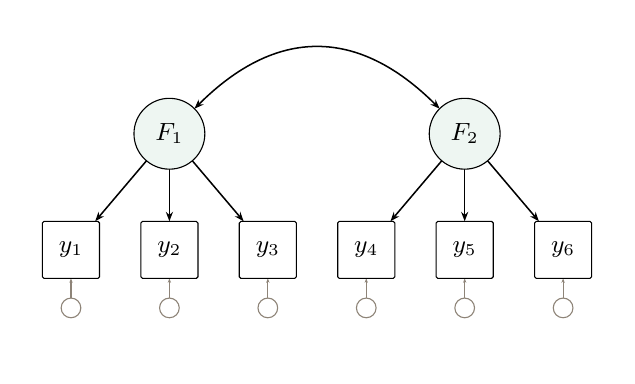
\begin{tikzpicture}[x=1cm, y=1cm,
    obs/.style={draw, rounded corners=0.6pt, minimum size=0.725cm, inner sep=0pt, fill=white, font=\fontsize{9.0}{10}\selectfont},
    lat/.style={draw, circle, minimum size=0.900cm, inner sep=0pt, fill=latfill, font=\fontsize{9.0}{10}\selectfont},
    resid/.style={draw=residc, line width=0.4pt}, residarrow/.style={draw=residc, -{Stealth[length=1.6pt]}, line width=0.4pt},
    path/.style={-{Stealth[length=3.4pt]}, line width=0.55pt},
    cov/.style={{Stealth[length=3.4pt]}-{Stealth[length=3.4pt]}, line width=0.55pt},
    net/.style={draw=netc, line width=1.1pt, line cap=round},
    elabel/.style={font=\scriptsize\itshape, fill=white, inner sep=0.6pt}]
\useasboundingbox (-0.550,-0.053) rectangle (6.800,-4.219);
\draw[resid] (0.000,-3.612) circle (0.125);
\draw[residarrow] (0.000,-3.487) -- (0.000,-3.237);
\draw[resid] (1.250,-3.612) circle (0.125);
\draw[residarrow] (1.250,-3.487) -- (1.250,-3.237);
\draw[resid] (2.500,-3.612) circle (0.125);
\draw[residarrow] (2.500,-3.487) -- (2.500,-3.237);
\draw[resid] (3.750,-3.612) circle (0.125);
\draw[residarrow] (3.750,-3.487) -- (3.750,-3.237);
\draw[resid] (5.000,-3.612) circle (0.125);
\draw[residarrow] (5.000,-3.487) -- (5.000,-3.237);
\draw[resid] (6.250,-3.612) circle (0.125);
\draw[residarrow] (6.250,-3.487) -- (6.250,-3.237);
\draw[path] (0.959,-1.743) -- (0.307,-2.512);
\draw[path] (1.250,-1.850) -- (1.250,-2.512);
\draw[path] (1.541,-1.743) -- (2.193,-2.512);
\draw[path] (4.709,-1.743) -- (4.057,-2.512);
\draw[path] (5.000,-1.850) -- (5.000,-2.512);
\draw[path] (5.291,-1.743) -- (5.943,-2.512);
\draw[cov] (1.568,-1.082) .. controls (2.606,-0.044) and (3.644,-0.044) .. (4.682,-1.082);
\node[obs] at (0.000,-2.875) {$y_{1}$};
\node[obs] at (1.250,-2.875) {$y_{2}$};
\node[obs] at (2.500,-2.875) {$y_{3}$};
\node[obs] at (3.750,-2.875) {$y_{4}$};
\node[obs] at (5.000,-2.875) {$y_{5}$};
\node[obs] at (6.250,-2.875) {$y_{6}$};
\node[lat] at (1.250,-1.400) {$F_{1}$};
\node[lat] at (5.000,-1.400) {$F_{2}$};
\end{tikzpicture}\\[1pt]{\scriptsize \texttt{F1 =\char`\~{} y1 + y2 + y3; F2 =\char`\~{} y4 + y5 + y6; F1 \char`\~{}\char`\~{} F2}}\end{minipage}
\par\bigskip
\noindent\textbf{Claim.} $B \nest A$, $A \nnest B$: \textbf{B is nested in A} (strictly).\par\smallskip
\noindent\textbf{Proof.} (i) $A\nnest B$ by Lemma~D: the Jacobian of model $A$ has rank 14 at the rational point listed in Appendix~B, while model $B$ has only $q_B=13$ free parameters.\par\smallskip
\noindent(ii) $B\nest A$. Fix $\theta_{34}=0$ in $A$ (Lemma~R).\hfill$\square$\par\medskip
\noindent{\small\textit{In the game:} A is B plus one residual covariance (y3 ↔ y4). Fix it to zero and you get B, so B is nested in A.}

\clearpage
\section*{E12 \quad Correlated or independent predictors}
\addcontentsline{toc}{subsection}{E12\quad Correlated or independent predictors}
\noindent\textit{Level: Easy.} Observed variables: $A, B, C$ ($p=3$, 6 moments).\par\medskip
\noindent\begin{minipage}[t]{0.49\textwidth}\centering\textbf{\color{acol}Model A} \;{\small $q_A=6$}\\[2pt]
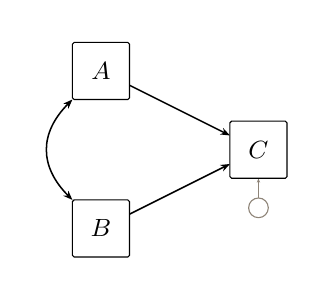
\begin{tikzpicture}[x=1cm, y=1cm,
    obs/.style={draw, rounded corners=0.6pt, minimum size=0.725cm, inner sep=0pt, fill=white, font=\fontsize{9.0}{10}\selectfont},
    lat/.style={draw, circle, minimum size=0.900cm, inner sep=0pt, fill=latfill, font=\fontsize{9.0}{10}\selectfont},
    resid/.style={draw=residc, line width=0.4pt}, residarrow/.style={draw=residc, -{Stealth[length=1.6pt]}, line width=0.4pt},
    path/.style={-{Stealth[length=3.4pt]}, line width=0.55pt},
    cov/.style={{Stealth[length=3.4pt]}-{Stealth[length=3.4pt]}, line width=0.55pt},
    net/.style={draw=netc, line width=1.1pt, line cap=round},
    elabel/.style={font=\scriptsize\itshape, fill=white, inner sep=0.6pt}]
\useasboundingbox (-0.931,0.550) rectangle (2.550,-2.550);
\draw[resid] (2.000,-1.738) circle (0.125);
\draw[residarrow] (2.000,-1.613) -- (2.000,-1.363);
\draw[path] (0.362,-0.181) -- (1.638,-0.819);
\draw[path] (0.362,-1.819) -- (1.638,-1.181);
\draw[cov] (-0.362,-0.362) .. controls (-0.787,-0.787) and (-0.787,-1.213) .. (-0.362,-1.638);
\node[obs] at (0.000,0.000) {$A$};
\node[obs] at (0.000,-2.000) {$B$};
\node[obs] at (2.000,-1.000) {$C$};
\end{tikzpicture}\\[1pt]{\scriptsize \texttt{C \char`\~{} A + B; A \char`\~{}\char`\~{} B}}\end{minipage}\hfill
\begin{minipage}[t]{0.49\textwidth}\centering\textbf{\color{bcol}Model B} \;{\small $q_B=5$}\\[2pt]
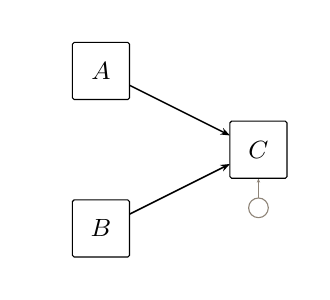
\begin{tikzpicture}[x=1cm, y=1cm,
    obs/.style={draw, rounded corners=0.6pt, minimum size=0.725cm, inner sep=0pt, fill=white, font=\fontsize{9.0}{10}\selectfont},
    lat/.style={draw, circle, minimum size=0.900cm, inner sep=0pt, fill=latfill, font=\fontsize{9.0}{10}\selectfont},
    resid/.style={draw=residc, line width=0.4pt}, residarrow/.style={draw=residc, -{Stealth[length=1.6pt]}, line width=0.4pt},
    path/.style={-{Stealth[length=3.4pt]}, line width=0.55pt},
    cov/.style={{Stealth[length=3.4pt]}-{Stealth[length=3.4pt]}, line width=0.55pt},
    net/.style={draw=netc, line width=1.1pt, line cap=round},
    elabel/.style={font=\scriptsize\itshape, fill=white, inner sep=0.6pt}]
\useasboundingbox (-0.931,0.550) rectangle (2.550,-2.550);
\draw[resid] (2.000,-1.738) circle (0.125);
\draw[residarrow] (2.000,-1.613) -- (2.000,-1.363);
\draw[path] (0.362,-0.181) -- (1.638,-0.819);
\draw[path] (0.362,-1.819) -- (1.638,-1.181);
\node[obs] at (0.000,0.000) {$A$};
\node[obs] at (0.000,-2.000) {$B$};
\node[obs] at (2.000,-1.000) {$C$};
\end{tikzpicture}\\[1pt]{\scriptsize \texttt{C \char`\~{} A + B}}\end{minipage}
\par\bigskip
\noindent\textbf{Claim.} $B \nest A$, $A \nnest B$: \textbf{B is nested in A} (strictly).\par\smallskip
\noindent\textbf{Proof.} (i) $A\nnest B$ by Lemma~D: the Jacobian of model $A$ has rank 6 at the rational point listed in Appendix~B, while model $B$ has only $q_B=5$ free parameters.\par\smallskip
\noindent(ii) $B\nest A$. Fix $\mathrm{Cov}(A,B)=0$ in $A$ (Lemma~R).\hfill$\square$\par\medskip
\noindent{\small\textit{In the game:} B is A with the covariance between the predictors fixed to zero (A and B independent). B is nested in A.}

\clearpage
\section*{E13 \quad Equal loadings}
\addcontentsline{toc}{subsection}{E13\quad Equal loadings}
\noindent\textit{Level: Easy.} Observed variables: $y_{1}, y_{2}, y_{3}, y_{4}$ ($p=4$, 10 moments).\par\medskip
\noindent\begin{minipage}[t]{0.49\textwidth}\centering\textbf{\color{acol}Model A} \;{\small $q_A=8$}\\[2pt]
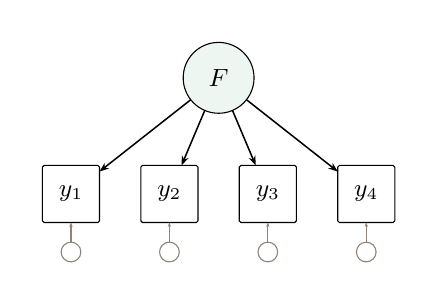
\begin{tikzpicture}[x=1cm, y=1cm,
    obs/.style={draw, rounded corners=0.6pt, minimum size=0.725cm, inner sep=0pt, fill=white, font=\fontsize{9.0}{10}\selectfont},
    lat/.style={draw, circle, minimum size=0.900cm, inner sep=0pt, fill=latfill, font=\fontsize{9.0}{10}\selectfont},
    resid/.style={draw=residc, line width=0.4pt}, residarrow/.style={draw=residc, -{Stealth[length=1.6pt]}, line width=0.4pt},
    path/.style={-{Stealth[length=3.4pt]}, line width=0.55pt},
    cov/.style={{Stealth[length=3.4pt]}-{Stealth[length=3.4pt]}, line width=0.55pt},
    net/.style={draw=netc, line width=1.1pt, line cap=round},
    elabel/.style={font=\scriptsize\itshape, fill=white, inner sep=0.6pt}]
\useasboundingbox (-0.550,-0.763) rectangle (4.300,-3.925);
\draw[resid] (0.000,-3.612) circle (0.125);
\draw[residarrow] (0.000,-3.487) -- (0.000,-3.237);
\draw[resid] (1.250,-3.612) circle (0.125);
\draw[residarrow] (1.250,-3.487) -- (1.250,-3.237);
\draw[resid] (2.500,-3.612) circle (0.125);
\draw[residarrow] (2.500,-3.487) -- (2.500,-3.237);
\draw[resid] (3.750,-3.612) circle (0.125);
\draw[residarrow] (3.750,-3.487) -- (3.750,-3.237);
\draw[path] (1.521,-1.678) -- (0.362,-2.590);
\draw[path] (1.699,-1.814) -- (1.404,-2.512);
\draw[path] (2.051,-1.814) -- (2.346,-2.512);
\draw[path] (2.229,-1.678) -- (3.388,-2.590);
\node[obs] at (0.000,-2.875) {$y_{1}$};
\node[obs] at (1.250,-2.875) {$y_{2}$};
\node[obs] at (2.500,-2.875) {$y_{3}$};
\node[obs] at (3.750,-2.875) {$y_{4}$};
\node[lat] at (1.875,-1.400) {$F$};
\end{tikzpicture}\\[1pt]{\scriptsize \texttt{F =\char`\~{} y1 + y2 + y3 + y4}}\end{minipage}\hfill
\begin{minipage}[t]{0.49\textwidth}\centering\textbf{\color{bcol}Model B} \;{\small $q_B=6$}\\[2pt]
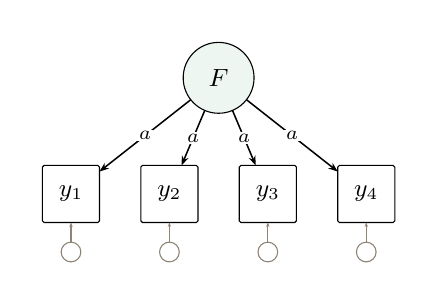
\begin{tikzpicture}[x=1cm, y=1cm,
    obs/.style={draw, rounded corners=0.6pt, minimum size=0.725cm, inner sep=0pt, fill=white, font=\fontsize{9.0}{10}\selectfont},
    lat/.style={draw, circle, minimum size=0.900cm, inner sep=0pt, fill=latfill, font=\fontsize{9.0}{10}\selectfont},
    resid/.style={draw=residc, line width=0.4pt}, residarrow/.style={draw=residc, -{Stealth[length=1.6pt]}, line width=0.4pt},
    path/.style={-{Stealth[length=3.4pt]}, line width=0.55pt},
    cov/.style={{Stealth[length=3.4pt]}-{Stealth[length=3.4pt]}, line width=0.55pt},
    net/.style={draw=netc, line width=1.1pt, line cap=round},
    elabel/.style={font=\scriptsize\itshape, fill=white, inner sep=0.6pt}]
\useasboundingbox (-0.550,-0.763) rectangle (4.300,-3.925);
\draw[resid] (0.000,-3.612) circle (0.125);
\draw[residarrow] (0.000,-3.487) -- (0.000,-3.237);
\draw[resid] (1.250,-3.612) circle (0.125);
\draw[residarrow] (1.250,-3.487) -- (1.250,-3.237);
\draw[resid] (2.500,-3.612) circle (0.125);
\draw[residarrow] (2.500,-3.487) -- (2.500,-3.237);
\draw[resid] (3.750,-3.612) circle (0.125);
\draw[residarrow] (3.750,-3.487) -- (3.750,-3.237);
\draw[path] (1.521,-1.678) -- (0.362,-2.590) node[elabel,pos=0.5] {$a$};
\draw[path] (1.699,-1.814) -- (1.404,-2.512) node[elabel,pos=0.5] {$a$};
\draw[path] (2.051,-1.814) -- (2.346,-2.512) node[elabel,pos=0.5] {$a$};
\draw[path] (2.229,-1.678) -- (3.388,-2.590) node[elabel,pos=0.5] {$a$};
\node[obs] at (0.000,-2.875) {$y_{1}$};
\node[obs] at (1.250,-2.875) {$y_{2}$};
\node[obs] at (2.500,-2.875) {$y_{3}$};
\node[obs] at (3.750,-2.875) {$y_{4}$};
\node[lat] at (1.875,-1.400) {$F$};
\end{tikzpicture}\\[1pt]{\scriptsize \texttt{F =\char`\~{} a*y1 + a*y2 + a*y3 + a*y4}}\end{minipage}
\par\bigskip
\noindent\textbf{Claim.} $B \nest A$, $A \nnest B$: \textbf{B is nested in A} (strictly).\par\smallskip
\noindent\textbf{Proof.} (i) $A\nnest B$ by Lemma~D: the Jacobian of model $A$ has rank 8 at the rational point listed in Appendix~B, while model $B$ has only $q_B=6$ free parameters.\par\smallskip
\noindent(ii) $B\nest A$. $B$ is $A$ with the equality constraints $\lambda_1=\lambda_2=\lambda_3=\lambda_4$ (Lemma~R; with free factor variance the common loading can be set to 1).\hfill$\square$\par\medskip
\noindent{\small\textit{In the game:} B forces all loadings to be equal (label a). That is a special case of A, where the loadings are free: B is nested in A.}

\clearpage
\section*{E14 \quad A direct effect of the covariate}
\addcontentsline{toc}{subsection}{E14\quad A direct effect of the covariate}
\noindent\textit{Level: Easy.} Observed variables: $X, y_{1}, y_{2}, y_{3}$ ($p=4$, 10 moments).\par\medskip
\noindent\begin{minipage}[t]{0.49\textwidth}\centering\textbf{\color{acol}Model A} \;{\small $q_A=9$}\\[2pt]
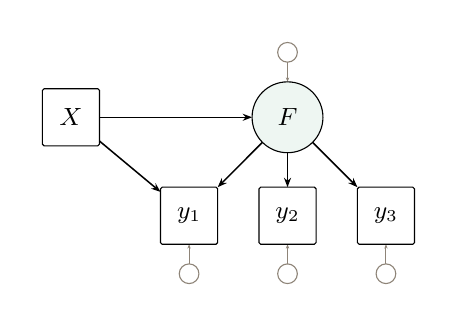
\begin{tikzpicture}[x=1cm, y=1cm,
    obs/.style={draw, rounded corners=0.6pt, minimum size=0.725cm, inner sep=0pt, fill=white, font=\fontsize{9.0}{10}\selectfont},
    lat/.style={draw, circle, minimum size=0.900cm, inner sep=0pt, fill=latfill, font=\fontsize{9.0}{10}\selectfont},
    resid/.style={draw=residc, line width=0.4pt}, residarrow/.style={draw=residc, -{Stealth[length=1.6pt]}, line width=0.4pt},
    path/.style={-{Stealth[length=3.4pt]}, line width=0.55pt},
    cov/.style={{Stealth[length=3.4pt]}-{Stealth[length=3.4pt]}, line width=0.55pt},
    net/.style={draw=netc, line width=1.1pt, line cap=round},
    elabel/.style={font=\scriptsize\itshape, fill=white, inner sep=0.6pt}]
\useasboundingbox (-0.550,-0.112) rectangle (4.550,-3.550);
\draw[resid] (1.500,-3.237) circle (0.125);
\draw[residarrow] (1.500,-3.112) -- (1.500,-2.862);
\draw[resid] (2.750,-3.237) circle (0.125);
\draw[residarrow] (2.750,-3.112) -- (2.750,-2.862);
\draw[resid] (4.000,-3.237) circle (0.125);
\draw[residarrow] (4.000,-3.112) -- (4.000,-2.862);
\draw[resid] (2.750,-0.425) circle (0.125);
\draw[residarrow] (2.750,-0.550) -- (2.750,-0.800);
\draw[path] (2.432,-1.568) -- (1.863,-2.138);
\draw[path] (2.750,-1.700) -- (2.750,-2.138);
\draw[path] (3.068,-1.568) -- (3.638,-2.138);
\draw[path] (0.362,-1.250) -- (2.300,-1.250);
\draw[path] (0.362,-1.552) -- (1.137,-2.198);
\node[obs] at (0.000,-1.250) {$X$};
\node[obs] at (1.500,-2.500) {$y_{1}$};
\node[obs] at (2.750,-2.500) {$y_{2}$};
\node[obs] at (4.000,-2.500) {$y_{3}$};
\node[lat] at (2.750,-1.250) {$F$};
\end{tikzpicture}\\[1pt]{\scriptsize \texttt{F =\char`\~{} y1 + y2 + y3; F \char`\~{} X; y1 \char`\~{} X}}\end{minipage}\hfill
\begin{minipage}[t]{0.49\textwidth}\centering\textbf{\color{bcol}Model B} \;{\small $q_B=8$}\\[2pt]
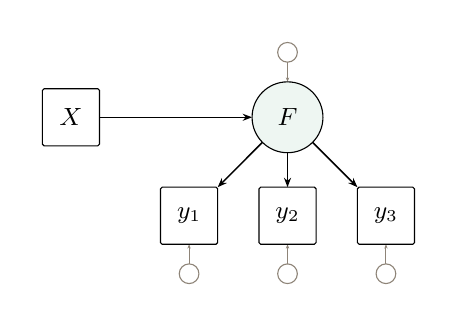
\begin{tikzpicture}[x=1cm, y=1cm,
    obs/.style={draw, rounded corners=0.6pt, minimum size=0.725cm, inner sep=0pt, fill=white, font=\fontsize{9.0}{10}\selectfont},
    lat/.style={draw, circle, minimum size=0.900cm, inner sep=0pt, fill=latfill, font=\fontsize{9.0}{10}\selectfont},
    resid/.style={draw=residc, line width=0.4pt}, residarrow/.style={draw=residc, -{Stealth[length=1.6pt]}, line width=0.4pt},
    path/.style={-{Stealth[length=3.4pt]}, line width=0.55pt},
    cov/.style={{Stealth[length=3.4pt]}-{Stealth[length=3.4pt]}, line width=0.55pt},
    net/.style={draw=netc, line width=1.1pt, line cap=round},
    elabel/.style={font=\scriptsize\itshape, fill=white, inner sep=0.6pt}]
\useasboundingbox (-0.550,-0.112) rectangle (4.550,-3.550);
\draw[resid] (1.500,-3.237) circle (0.125);
\draw[residarrow] (1.500,-3.112) -- (1.500,-2.862);
\draw[resid] (2.750,-3.237) circle (0.125);
\draw[residarrow] (2.750,-3.112) -- (2.750,-2.862);
\draw[resid] (4.000,-3.237) circle (0.125);
\draw[residarrow] (4.000,-3.112) -- (4.000,-2.862);
\draw[resid] (2.750,-0.425) circle (0.125);
\draw[residarrow] (2.750,-0.550) -- (2.750,-0.800);
\draw[path] (2.432,-1.568) -- (1.863,-2.138);
\draw[path] (2.750,-1.700) -- (2.750,-2.138);
\draw[path] (3.068,-1.568) -- (3.638,-2.138);
\draw[path] (0.362,-1.250) -- (2.300,-1.250);
\node[obs] at (0.000,-1.250) {$X$};
\node[obs] at (1.500,-2.500) {$y_{1}$};
\node[obs] at (2.750,-2.500) {$y_{2}$};
\node[obs] at (4.000,-2.500) {$y_{3}$};
\node[lat] at (2.750,-1.250) {$F$};
\end{tikzpicture}\\[1pt]{\scriptsize \texttt{F =\char`\~{} y1 + y2 + y3; F \char`\~{} X}}\end{minipage}
\par\bigskip
\noindent\textbf{Claim.} $B \nest A$, $A \nnest B$: \textbf{B is nested in A} (strictly).\par\smallskip
\noindent\textbf{Proof.} (i) $A\nnest B$ by Lemma~D: the Jacobian of model $A$ has rank 9 at the rational point listed in Appendix~B, while model $B$ has only $q_B=8$ free parameters.\par\smallskip
\noindent(ii) $B\nest A$. Fix the direct effect $X\to y_1$ in $A$ to 0 (Lemma~R).\hfill$\square$\par\medskip
\noindent{\small\textit{In the game:} A adds a direct effect of the covariate X on item y1. Fixing it to zero gives B, so B is nested in A.}

\clearpage
\section*{E15 \quad The independence model}
\addcontentsline{toc}{subsection}{E15\quad The independence model}
\noindent\textit{Level: Easy.} Observed variables: $A, B, C$ ($p=3$, 6 moments).\par\medskip
\noindent\begin{minipage}[t]{0.49\textwidth}\centering\textbf{\color{acol}Model A} \;{\small $q_A=5$}\\[2pt]
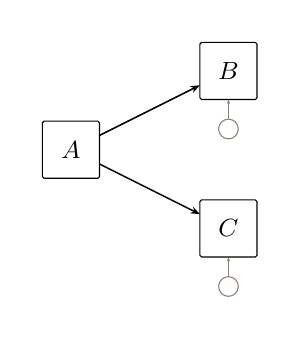
\begin{tikzpicture}[x=1cm, y=1cm,
    obs/.style={draw, rounded corners=0.6pt, minimum size=0.725cm, inner sep=0pt, fill=white, font=\fontsize{9.0}{10}\selectfont},
    lat/.style={draw, circle, minimum size=0.900cm, inner sep=0pt, fill=latfill, font=\fontsize{9.0}{10}\selectfont},
    resid/.style={draw=residc, line width=0.4pt}, residarrow/.style={draw=residc, -{Stealth[length=1.6pt]}, line width=0.4pt},
    path/.style={-{Stealth[length=3.4pt]}, line width=0.55pt},
    cov/.style={{Stealth[length=3.4pt]}-{Stealth[length=3.4pt]}, line width=0.55pt},
    net/.style={draw=netc, line width=1.1pt, line cap=round},
    elabel/.style={font=\scriptsize\itshape, fill=white, inner sep=0.6pt}]
\useasboundingbox (-0.550,0.550) rectangle (2.550,-3.050);
\draw[resid] (2.000,-0.737) circle (0.125);
\draw[residarrow] (2.000,-0.613) -- (2.000,-0.362);
\draw[resid] (2.000,-2.737) circle (0.125);
\draw[residarrow] (2.000,-2.612) -- (2.000,-2.363);
\draw[path] (0.362,-0.819) -- (1.638,-0.181);
\draw[path] (0.362,-1.181) -- (1.638,-1.819);
\node[obs] at (0.000,-1.000) {$A$};
\node[obs] at (2.000,0.000) {$B$};
\node[obs] at (2.000,-2.000) {$C$};
\end{tikzpicture}\\[1pt]{\scriptsize \texttt{B \char`\~{} A; C \char`\~{} A}}\end{minipage}\hfill
\begin{minipage}[t]{0.49\textwidth}\centering\textbf{\color{bcol}Model B} \;{\small $q_B=3$}\\[2pt]
\begin{tikzpicture}[x=1cm, y=1cm,
    obs/.style={draw, rounded corners=0.6pt, minimum size=0.725cm, inner sep=0pt, fill=white, font=\fontsize{9.0}{10}\selectfont},
    lat/.style={draw, circle, minimum size=0.900cm, inner sep=0pt, fill=latfill, font=\fontsize{9.0}{10}\selectfont},
    resid/.style={draw=residc, line width=0.4pt}, residarrow/.style={draw=residc, -{Stealth[length=1.6pt]}, line width=0.4pt},
    path/.style={-{Stealth[length=3.4pt]}, line width=0.55pt},
    cov/.style={{Stealth[length=3.4pt]}-{Stealth[length=3.4pt]}, line width=0.55pt},
    net/.style={draw=netc, line width=1.1pt, line cap=round},
    elabel/.style={font=\scriptsize\itshape, fill=white, inner sep=0.6pt}]
\useasboundingbox (-0.550,0.550) rectangle (2.550,-3.050);
\node[obs] at (0.000,-1.000) {$A$};
\node[obs] at (2.000,0.000) {$B$};
\node[obs] at (2.000,-2.000) {$C$};
\end{tikzpicture}\\[1pt]{\scriptsize \texttt{(no paths: variances only)}}\end{minipage}
\par\bigskip
\noindent\textbf{Claim.} $B \nest A$, $A \nnest B$: \textbf{B is nested in A} (strictly).\par\smallskip
\noindent\textbf{Proof.} (i) $A\nnest B$ by Lemma~D: the Jacobian of model $A$ has rank 5 at the rational point listed in Appendix~B, while model $B$ has only $q_B=3$ free parameters.\par\smallskip
\noindent(ii) $B\nest A$. Fix both regression coefficients in $A$ to 0 (Lemma~R): $B$ only has variances.\hfill$\square$\par\medskip
\noindent{\small\textit{In the game:} B has no paths at all: only variances (the independence or "baseline" model). It is nested in every model with the same variables, including A.}

\clearpage
\section*{E16 \quad Chain versus collider}
\addcontentsline{toc}{subsection}{E16\quad Chain versus collider}
\noindent\textit{Level: Easy.} Observed variables: $A, B, C$ ($p=3$, 6 moments).\par\medskip
\noindent\begin{minipage}[t]{0.49\textwidth}\centering\textbf{\color{acol}Model A} \;{\small $q_A=5$}\\[2pt]
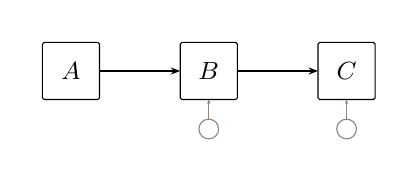
\begin{tikzpicture}[x=1cm, y=1cm,
    obs/.style={draw, rounded corners=0.6pt, minimum size=0.725cm, inner sep=0pt, fill=white, font=\fontsize{9.0}{10}\selectfont},
    lat/.style={draw, circle, minimum size=0.900cm, inner sep=0pt, fill=latfill, font=\fontsize{9.0}{10}\selectfont},
    resid/.style={draw=residc, line width=0.4pt}, residarrow/.style={draw=residc, -{Stealth[length=1.6pt]}, line width=0.4pt},
    path/.style={-{Stealth[length=3.4pt]}, line width=0.55pt},
    cov/.style={{Stealth[length=3.4pt]}-{Stealth[length=3.4pt]}, line width=0.55pt},
    net/.style={draw=netc, line width=1.1pt, line cap=round},
    elabel/.style={font=\scriptsize\itshape, fill=white, inner sep=0.6pt}]
\useasboundingbox (-0.550,0.550) rectangle (4.050,-1.050);
\draw[resid] (1.750,-0.737) circle (0.125);
\draw[residarrow] (1.750,-0.613) -- (1.750,-0.362);
\draw[resid] (3.500,-0.737) circle (0.125);
\draw[residarrow] (3.500,-0.613) -- (3.500,-0.362);
\draw[path] (0.362,0.000) -- (1.387,0.000);
\draw[path] (2.112,0.000) -- (3.137,0.000);
\node[obs] at (0.000,0.000) {$A$};
\node[obs] at (1.750,0.000) {$B$};
\node[obs] at (3.500,0.000) {$C$};
\end{tikzpicture}\\[1pt]{\scriptsize \texttt{B \char`\~{} A; C \char`\~{} B}}\end{minipage}\hfill
\begin{minipage}[t]{0.49\textwidth}\centering\textbf{\color{bcol}Model B} \;{\small $q_B=5$}\\[2pt]
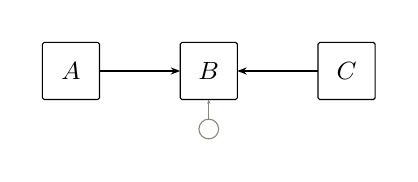
\begin{tikzpicture}[x=1cm, y=1cm,
    obs/.style={draw, rounded corners=0.6pt, minimum size=0.725cm, inner sep=0pt, fill=white, font=\fontsize{9.0}{10}\selectfont},
    lat/.style={draw, circle, minimum size=0.900cm, inner sep=0pt, fill=latfill, font=\fontsize{9.0}{10}\selectfont},
    resid/.style={draw=residc, line width=0.4pt}, residarrow/.style={draw=residc, -{Stealth[length=1.6pt]}, line width=0.4pt},
    path/.style={-{Stealth[length=3.4pt]}, line width=0.55pt},
    cov/.style={{Stealth[length=3.4pt]}-{Stealth[length=3.4pt]}, line width=0.55pt},
    net/.style={draw=netc, line width=1.1pt, line cap=round},
    elabel/.style={font=\scriptsize\itshape, fill=white, inner sep=0.6pt}]
\useasboundingbox (-0.550,0.550) rectangle (4.050,-1.050);
\draw[resid] (1.750,-0.737) circle (0.125);
\draw[residarrow] (1.750,-0.613) -- (1.750,-0.362);
\draw[path] (0.362,0.000) -- (1.387,0.000);
\draw[path] (3.137,0.000) -- (2.112,0.000);
\node[obs] at (0.000,0.000) {$A$};
\node[obs] at (1.750,0.000) {$B$};
\node[obs] at (3.500,0.000) {$C$};
\end{tikzpicture}\\[1pt]{\scriptsize \texttt{B \char`\~{} A + C}}\end{minipage}
\par\bigskip
\noindent\textbf{Claim.} $A \nnest B$ and $B \nnest A$: \textbf{neither} is nested in the other.\par\smallskip
\noindent\textbf{Proof.} (i) $A\nnest B$ by Lemma~S with $f(\Sigma)=\sigma_{AC}$. In $B$, $A$ and $C$ are exogenous and not connected, so $\sigma_{AC}=0$. So $f\equiv0$ on $\mathcal M_B$, whereas in model $A$, $f=\beta_{BA}\beta_{CB}\,\mathrm{Var}(A)\neq0$ for generic parameters; e.g.\ at the point of Appendix~B, $f=0.3000\neq0$.\par\smallskip
\noindent(ii) $B\nnest A$ by Lemma~S with $f(\Sigma)=\sigma_{AC}\sigma_{BB} - \sigma_{AB}\sigma_{BC}$. In $A$, $\sigma_{AC}=\beta_{CB}\sigma_{AB}$ and $\sigma_{BC}=\beta_{CB}\sigma_{BB}$. So $f\equiv0$ on $\mathcal M_A$, whereas in model $B$, $f=-\sigma_{AB}\sigma_{BC}\neq0$ for generic parameters; e.g.\ at the point of Appendix~B, $f=-0.2700\neq0$.\hfill$\square$\par\medskip
\noindent{\small\textit{In the game:} The chain says A and C are independent given B; the collider says A and C are independent (period), but dependent given B. Each restriction is violated by the other model.}

\clearpage
\section*{E17 \quad Two different residual covariances}
\addcontentsline{toc}{subsection}{E17\quad Two different residual covariances}
\noindent\textit{Level: Easy.} Observed variables: $y_{1}, y_{2}, y_{3}, y_{4}, y_{5}, y_{6}$ ($p=6$, 21 moments).\par\medskip
\noindent\begin{minipage}[t]{0.49\textwidth}\centering\textbf{\color{acol}Model A} \;{\small $q_A=14$}\\[2pt]
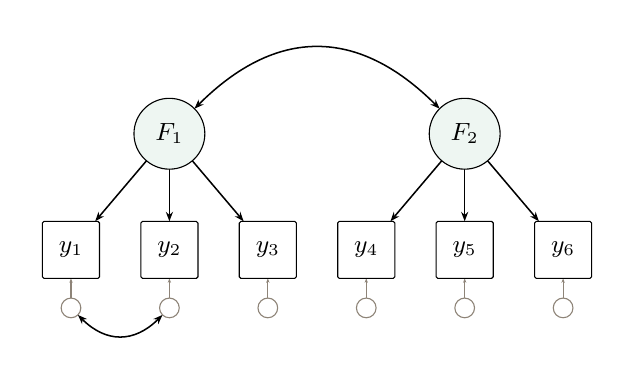
\begin{tikzpicture}[x=1cm, y=1cm,
    obs/.style={draw, rounded corners=0.6pt, minimum size=0.725cm, inner sep=0pt, fill=white, font=\fontsize{9.0}{10}\selectfont},
    lat/.style={draw, circle, minimum size=0.900cm, inner sep=0pt, fill=latfill, font=\fontsize{9.0}{10}\selectfont},
    resid/.style={draw=residc, line width=0.4pt}, residarrow/.style={draw=residc, -{Stealth[length=1.6pt]}, line width=0.4pt},
    path/.style={-{Stealth[length=3.4pt]}, line width=0.55pt},
    cov/.style={{Stealth[length=3.4pt]}-{Stealth[length=3.4pt]}, line width=0.55pt},
    net/.style={draw=netc, line width=1.1pt, line cap=round},
    elabel/.style={font=\scriptsize\itshape, fill=white, inner sep=0.6pt}]
\useasboundingbox (-0.550,-0.053) rectangle (6.800,-4.219);
\draw[resid] (0.000,-3.612) circle (0.125);
\draw[residarrow] (0.000,-3.487) -- (0.000,-3.237);
\draw[resid] (1.250,-3.612) circle (0.125);
\draw[residarrow] (1.250,-3.487) -- (1.250,-3.237);
\draw[resid] (2.500,-3.612) circle (0.125);
\draw[residarrow] (2.500,-3.487) -- (2.500,-3.237);
\draw[resid] (3.750,-3.612) circle (0.125);
\draw[residarrow] (3.750,-3.487) -- (3.750,-3.237);
\draw[resid] (5.000,-3.612) circle (0.125);
\draw[residarrow] (5.000,-3.487) -- (5.000,-3.237);
\draw[resid] (6.250,-3.612) circle (0.125);
\draw[residarrow] (6.250,-3.487) -- (6.250,-3.237);
\draw[path] (0.959,-1.743) -- (0.307,-2.512);
\draw[path] (1.250,-1.850) -- (1.250,-2.512);
\draw[path] (1.541,-1.743) -- (2.193,-2.512);
\draw[path] (4.709,-1.743) -- (4.057,-2.512);
\draw[path] (5.000,-1.850) -- (5.000,-2.512);
\draw[path] (5.291,-1.743) -- (5.943,-2.512);
\draw[cov] (1.568,-1.082) .. controls (2.606,-0.044) and (3.644,-0.044) .. (4.682,-1.082);
\draw[cov] (0.088,-3.701) .. controls (0.446,-4.059) and (0.804,-4.059) .. (1.162,-3.701);
\node[obs] at (0.000,-2.875) {$y_{1}$};
\node[obs] at (1.250,-2.875) {$y_{2}$};
\node[obs] at (2.500,-2.875) {$y_{3}$};
\node[obs] at (3.750,-2.875) {$y_{4}$};
\node[obs] at (5.000,-2.875) {$y_{5}$};
\node[obs] at (6.250,-2.875) {$y_{6}$};
\node[lat] at (1.250,-1.400) {$F_{1}$};
\node[lat] at (5.000,-1.400) {$F_{2}$};
\end{tikzpicture}\\[1pt]{\scriptsize \texttt{F1 =\char`\~{} y1 + y2 + y3; F2 =\char`\~{} y4 + y5 + y6; F1 \char`\~{}\char`\~{} F2; y1 \char`\~{}\char`\~{} y2}}\end{minipage}\hfill
\begin{minipage}[t]{0.49\textwidth}\centering\textbf{\color{bcol}Model B} \;{\small $q_B=14$}\\[2pt]
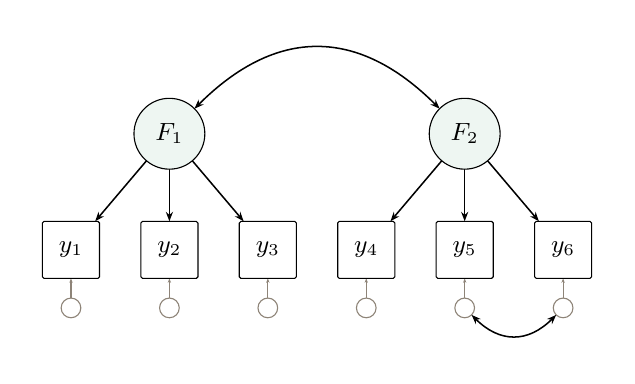
\begin{tikzpicture}[x=1cm, y=1cm,
    obs/.style={draw, rounded corners=0.6pt, minimum size=0.725cm, inner sep=0pt, fill=white, font=\fontsize{9.0}{10}\selectfont},
    lat/.style={draw, circle, minimum size=0.900cm, inner sep=0pt, fill=latfill, font=\fontsize{9.0}{10}\selectfont},
    resid/.style={draw=residc, line width=0.4pt}, residarrow/.style={draw=residc, -{Stealth[length=1.6pt]}, line width=0.4pt},
    path/.style={-{Stealth[length=3.4pt]}, line width=0.55pt},
    cov/.style={{Stealth[length=3.4pt]}-{Stealth[length=3.4pt]}, line width=0.55pt},
    net/.style={draw=netc, line width=1.1pt, line cap=round},
    elabel/.style={font=\scriptsize\itshape, fill=white, inner sep=0.6pt}]
\useasboundingbox (-0.550,-0.053) rectangle (6.800,-4.219);
\draw[resid] (0.000,-3.612) circle (0.125);
\draw[residarrow] (0.000,-3.487) -- (0.000,-3.237);
\draw[resid] (1.250,-3.612) circle (0.125);
\draw[residarrow] (1.250,-3.487) -- (1.250,-3.237);
\draw[resid] (2.500,-3.612) circle (0.125);
\draw[residarrow] (2.500,-3.487) -- (2.500,-3.237);
\draw[resid] (3.750,-3.612) circle (0.125);
\draw[residarrow] (3.750,-3.487) -- (3.750,-3.237);
\draw[resid] (5.000,-3.612) circle (0.125);
\draw[residarrow] (5.000,-3.487) -- (5.000,-3.237);
\draw[resid] (6.250,-3.612) circle (0.125);
\draw[residarrow] (6.250,-3.487) -- (6.250,-3.237);
\draw[path] (0.959,-1.743) -- (0.307,-2.512);
\draw[path] (1.250,-1.850) -- (1.250,-2.512);
\draw[path] (1.541,-1.743) -- (2.193,-2.512);
\draw[path] (4.709,-1.743) -- (4.057,-2.512);
\draw[path] (5.000,-1.850) -- (5.000,-2.512);
\draw[path] (5.291,-1.743) -- (5.943,-2.512);
\draw[cov] (1.568,-1.082) .. controls (2.606,-0.044) and (3.644,-0.044) .. (4.682,-1.082);
\draw[cov] (5.088,-3.701) .. controls (5.446,-4.059) and (5.804,-4.059) .. (6.162,-3.701);
\node[obs] at (0.000,-2.875) {$y_{1}$};
\node[obs] at (1.250,-2.875) {$y_{2}$};
\node[obs] at (2.500,-2.875) {$y_{3}$};
\node[obs] at (3.750,-2.875) {$y_{4}$};
\node[obs] at (5.000,-2.875) {$y_{5}$};
\node[obs] at (6.250,-2.875) {$y_{6}$};
\node[lat] at (1.250,-1.400) {$F_{1}$};
\node[lat] at (5.000,-1.400) {$F_{2}$};
\end{tikzpicture}\\[1pt]{\scriptsize \texttt{F1 =\char`\~{} y1 + y2 + y3; F2 =\char`\~{} y4 + y5 + y6; F1 \char`\~{}\char`\~{} F2; y5 \char`\~{}\char`\~{} y6}}\end{minipage}
\par\bigskip
\noindent\textbf{Claim.} $A \nnest B$ and $B \nnest A$: \textbf{neither} is nested in the other.\par\smallskip
\noindent\textbf{Proof.} (i) $A\nnest B$ by Lemma~S with $f(\Sigma)=\sigma_{12}\sigma_{35} - \sigma_{13}\sigma_{25}$. In $B$ these four covariances are products $\lambda_i\lambda_j\psi_{f(i)f(j)}$ (no residual covariance involved), and the two products are equal. So $f\equiv0$ on $\mathcal M_B$, whereas in model $A$, $f=\theta_{12}\lambda_3\lambda_5\psi_{12}\neq0$ for generic parameters; e.g.\ at the point of Appendix~B, $f=0.06480\neq0$.\par\smallskip
\noindent(ii) $B\nnest A$ by Lemma~S with $f(\Sigma)=\sigma_{56}\sigma_{24} - \sigma_{45}\sigma_{26}$. In $A$ these covariances are products of loadings and factor covariances (no $\theta_{56}$). So $f\equiv0$ on $\mathcal M_A$, whereas in model $B$, $f=\theta_{56}\lambda_2\lambda_4\psi_{12}\neq0$ for generic parameters; e.g.\ at the point of Appendix~B, $f=0.06000\neq0$.\hfill$\square$\par\medskip
\noindent{\small\textit{In the game:} Same number of parameters, but each model frees a residual covariance that the other fixes to zero. Neither can mimic the other.}

\clearpage
\section*{E18 \quad Two orthogonal factors versus one factor}
\addcontentsline{toc}{subsection}{E18\quad Two orthogonal factors versus one factor}
\noindent\textit{Level: Easy.} Observed variables: $y_{1}, y_{2}, y_{3}, y_{4}, y_{5}, y_{6}$ ($p=6$, 21 moments).\par\medskip
\noindent\begin{minipage}[t]{0.49\textwidth}\centering\textbf{\color{acol}Model A} \;{\small $q_A=12$}\\[2pt]
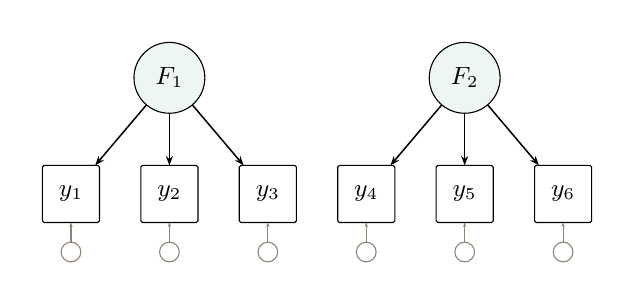
\begin{tikzpicture}[x=1cm, y=1cm,
    obs/.style={draw, rounded corners=0.6pt, minimum size=0.725cm, inner sep=0pt, fill=white, font=\fontsize{9.0}{10}\selectfont},
    lat/.style={draw, circle, minimum size=0.900cm, inner sep=0pt, fill=latfill, font=\fontsize{9.0}{10}\selectfont},
    resid/.style={draw=residc, line width=0.4pt}, residarrow/.style={draw=residc, -{Stealth[length=1.6pt]}, line width=0.4pt},
    path/.style={-{Stealth[length=3.4pt]}, line width=0.55pt},
    cov/.style={{Stealth[length=3.4pt]}-{Stealth[length=3.4pt]}, line width=0.55pt},
    net/.style={draw=netc, line width=1.1pt, line cap=round},
    elabel/.style={font=\scriptsize\itshape, fill=white, inner sep=0.6pt}]
\useasboundingbox (-0.550,-0.763) rectangle (6.800,-3.925);
\draw[resid] (0.000,-3.612) circle (0.125);
\draw[residarrow] (0.000,-3.487) -- (0.000,-3.237);
\draw[resid] (1.250,-3.612) circle (0.125);
\draw[residarrow] (1.250,-3.487) -- (1.250,-3.237);
\draw[resid] (2.500,-3.612) circle (0.125);
\draw[residarrow] (2.500,-3.487) -- (2.500,-3.237);
\draw[resid] (3.750,-3.612) circle (0.125);
\draw[residarrow] (3.750,-3.487) -- (3.750,-3.237);
\draw[resid] (5.000,-3.612) circle (0.125);
\draw[residarrow] (5.000,-3.487) -- (5.000,-3.237);
\draw[resid] (6.250,-3.612) circle (0.125);
\draw[residarrow] (6.250,-3.487) -- (6.250,-3.237);
\draw[path] (0.959,-1.743) -- (0.307,-2.512);
\draw[path] (1.250,-1.850) -- (1.250,-2.512);
\draw[path] (1.541,-1.743) -- (2.193,-2.512);
\draw[path] (4.709,-1.743) -- (4.057,-2.512);
\draw[path] (5.000,-1.850) -- (5.000,-2.512);
\draw[path] (5.291,-1.743) -- (5.943,-2.512);
\node[obs] at (0.000,-2.875) {$y_{1}$};
\node[obs] at (1.250,-2.875) {$y_{2}$};
\node[obs] at (2.500,-2.875) {$y_{3}$};
\node[obs] at (3.750,-2.875) {$y_{4}$};
\node[obs] at (5.000,-2.875) {$y_{5}$};
\node[obs] at (6.250,-2.875) {$y_{6}$};
\node[lat] at (1.250,-1.400) {$F_{1}$};
\node[lat] at (5.000,-1.400) {$F_{2}$};
\end{tikzpicture}\\[1pt]{\scriptsize \texttt{F1 =\char`\~{} y1 + y2 + y3; F2 =\char`\~{} y4 + y5 + y6}}\end{minipage}\hfill
\begin{minipage}[t]{0.49\textwidth}\centering\textbf{\color{bcol}Model B} \;{\small $q_B=12$}\\[2pt]
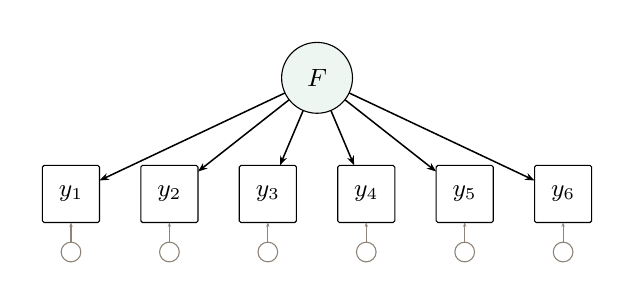
\begin{tikzpicture}[x=1cm, y=1cm,
    obs/.style={draw, rounded corners=0.6pt, minimum size=0.725cm, inner sep=0pt, fill=white, font=\fontsize{9.0}{10}\selectfont},
    lat/.style={draw, circle, minimum size=0.900cm, inner sep=0pt, fill=latfill, font=\fontsize{9.0}{10}\selectfont},
    resid/.style={draw=residc, line width=0.4pt}, residarrow/.style={draw=residc, -{Stealth[length=1.6pt]}, line width=0.4pt},
    path/.style={-{Stealth[length=3.4pt]}, line width=0.55pt},
    cov/.style={{Stealth[length=3.4pt]}-{Stealth[length=3.4pt]}, line width=0.55pt},
    net/.style={draw=netc, line width=1.1pt, line cap=round},
    elabel/.style={font=\scriptsize\itshape, fill=white, inner sep=0.6pt}]
\useasboundingbox (-0.550,-0.763) rectangle (6.800,-3.925);
\draw[resid] (0.000,-3.612) circle (0.125);
\draw[residarrow] (0.000,-3.487) -- (0.000,-3.237);
\draw[resid] (1.250,-3.612) circle (0.125);
\draw[residarrow] (1.250,-3.487) -- (1.250,-3.237);
\draw[resid] (2.500,-3.612) circle (0.125);
\draw[residarrow] (2.500,-3.487) -- (2.500,-3.237);
\draw[resid] (3.750,-3.612) circle (0.125);
\draw[residarrow] (3.750,-3.487) -- (3.750,-3.237);
\draw[resid] (5.000,-3.612) circle (0.125);
\draw[residarrow] (5.000,-3.487) -- (5.000,-3.237);
\draw[resid] (6.250,-3.612) circle (0.125);
\draw[residarrow] (6.250,-3.487) -- (6.250,-3.237);
\draw[path] (2.718,-1.592) -- (0.362,-2.704);
\draw[path] (2.771,-1.678) -- (1.613,-2.590);
\draw[path] (2.949,-1.814) -- (2.654,-2.512);
\draw[path] (3.301,-1.814) -- (3.596,-2.512);
\draw[path] (3.479,-1.678) -- (4.638,-2.590);
\draw[path] (3.532,-1.592) -- (5.888,-2.704);
\node[obs] at (0.000,-2.875) {$y_{1}$};
\node[obs] at (1.250,-2.875) {$y_{2}$};
\node[obs] at (2.500,-2.875) {$y_{3}$};
\node[obs] at (3.750,-2.875) {$y_{4}$};
\node[obs] at (5.000,-2.875) {$y_{5}$};
\node[obs] at (6.250,-2.875) {$y_{6}$};
\node[lat] at (3.125,-1.400) {$F$};
\end{tikzpicture}\\[1pt]{\scriptsize \texttt{F =\char`\~{} y1 + y2 + y3 + y4 + y5 + y6}}\end{minipage}
\par\bigskip
\noindent\textbf{Claim.} $A \nnest B$ and $B \nnest A$: \textbf{neither} is nested in the other.\par\smallskip
\noindent\textbf{Proof.} (i) $A\nnest B$ by Lemma~S with $f(\Sigma)=\sigma_{12}\sigma_{45} - \sigma_{14}\sigma_{25}$. One-factor model: every off-diagonal $\sigma_{ij}=\lambda_i\lambda_j\psi$, so all tetrads vanish. So $f\equiv0$ on $\mathcal M_B$, whereas in model $A$, $f=\lambda_1\lambda_2\lambda_4\lambda_5\psi_{11}\psi_{22}\neq0$ for generic parameters; e.g.\ at the point of Appendix~B, $f=1.440\neq0$.\par\smallskip
\noindent(ii) $B\nnest A$ by Lemma~S with $f(\Sigma)=\sigma_{14}$. Orthogonal factors: the two clusters are uncorrelated. So $f\equiv0$ on $\mathcal M_A$, whereas in model $B$, $f=\lambda_1\lambda_4\psi\neq0$ for generic parameters; e.g.\ at the point of Appendix~B, $f=1.200\neq0$.\hfill$\square$\par\medskip
\noindent{\small\textit{In the game:} A forces the two clusters to be uncorrelated; B forces all items through one factor, so the clusters must correlate. Neither restriction holds in the other model.}

\clearpage
\section*{E19 \quad Two different mediators}
\addcontentsline{toc}{subsection}{E19\quad Two different mediators}
\noindent\textit{Level: Easy.} Observed variables: $A, B, C$ ($p=3$, 6 moments).\par\medskip
\noindent\begin{minipage}[t]{0.49\textwidth}\centering\textbf{\color{acol}Model A} \;{\small $q_A=5$}\\[2pt]
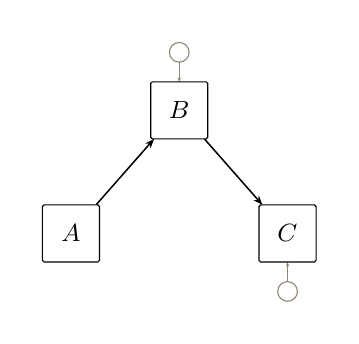
\begin{tikzpicture}[x=1cm, y=1cm,
    obs/.style={draw, rounded corners=0.6pt, minimum size=0.725cm, inner sep=0pt, fill=white, font=\fontsize{9.0}{10}\selectfont},
    lat/.style={draw, circle, minimum size=0.900cm, inner sep=0pt, fill=latfill, font=\fontsize{9.0}{10}\selectfont},
    resid/.style={draw=residc, line width=0.4pt}, residarrow/.style={draw=residc, -{Stealth[length=1.6pt]}, line width=0.4pt},
    path/.style={-{Stealth[length=3.4pt]}, line width=0.55pt},
    cov/.style={{Stealth[length=3.4pt]}-{Stealth[length=3.4pt]}, line width=0.55pt},
    net/.style={draw=netc, line width=1.1pt, line cap=round},
    elabel/.style={font=\scriptsize\itshape, fill=white, inner sep=0.6pt}]
\useasboundingbox (-0.550,1.050) rectangle (3.300,-2.612);
\draw[resid] (1.375,0.737) circle (0.125);
\draw[residarrow] (1.375,0.613) -- (1.375,0.362);
\draw[resid] (2.750,-2.300) circle (0.125);
\draw[residarrow] (2.750,-2.175) -- (2.750,-1.925);
\draw[path] (0.319,-1.200) -- (1.056,-0.362);
\draw[path] (1.694,-0.362) -- (2.431,-1.200);
\node[obs] at (0.000,-1.563) {$A$};
\node[obs] at (1.375,0.000) {$B$};
\node[obs] at (2.750,-1.563) {$C$};
\end{tikzpicture}\\[1pt]{\scriptsize \texttt{B \char`\~{} A; C \char`\~{} B}}\end{minipage}\hfill
\begin{minipage}[t]{0.49\textwidth}\centering\textbf{\color{bcol}Model B} \;{\small $q_B=5$}\\[2pt]
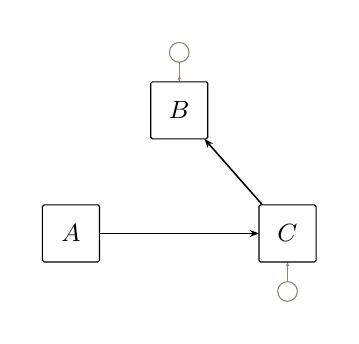
\begin{tikzpicture}[x=1cm, y=1cm,
    obs/.style={draw, rounded corners=0.6pt, minimum size=0.725cm, inner sep=0pt, fill=white, font=\fontsize{9.0}{10}\selectfont},
    lat/.style={draw, circle, minimum size=0.900cm, inner sep=0pt, fill=latfill, font=\fontsize{9.0}{10}\selectfont},
    resid/.style={draw=residc, line width=0.4pt}, residarrow/.style={draw=residc, -{Stealth[length=1.6pt]}, line width=0.4pt},
    path/.style={-{Stealth[length=3.4pt]}, line width=0.55pt},
    cov/.style={{Stealth[length=3.4pt]}-{Stealth[length=3.4pt]}, line width=0.55pt},
    net/.style={draw=netc, line width=1.1pt, line cap=round},
    elabel/.style={font=\scriptsize\itshape, fill=white, inner sep=0.6pt}]
\useasboundingbox (-0.550,1.050) rectangle (3.300,-2.612);
\draw[resid] (1.375,0.737) circle (0.125);
\draw[residarrow] (1.375,0.613) -- (1.375,0.362);
\draw[resid] (2.750,-2.300) circle (0.125);
\draw[residarrow] (2.750,-2.175) -- (2.750,-1.925);
\draw[path] (0.362,-1.563) -- (2.388,-1.563);
\draw[path] (2.431,-1.200) -- (1.694,-0.362);
\node[obs] at (0.000,-1.563) {$A$};
\node[obs] at (1.375,0.000) {$B$};
\node[obs] at (2.750,-1.563) {$C$};
\end{tikzpicture}\\[1pt]{\scriptsize \texttt{C \char`\~{} A; B \char`\~{} C}}\end{minipage}
\par\bigskip
\noindent\textbf{Claim.} $A \nnest B$ and $B \nnest A$: \textbf{neither} is nested in the other.\par\smallskip
\noindent\textbf{Proof.} (i) $A\nnest B$ by Lemma~S with $f(\Sigma)=\sigma_{AB}\sigma_{CC} - \sigma_{AC}\sigma_{BC}$. In $B$ ($A\to C\to B$), $A$ and $B$ are independent given $C$. So $f\equiv0$ on $\mathcal M_B$, whereas in model $A$ at the point of Appendix~B, $f=0.4500\neq0$.\par\smallskip
\noindent(ii) $B\nnest A$ by Lemma~S with $f(\Sigma)=\sigma_{AC}\sigma_{BB} - \sigma_{AB}\sigma_{BC}$. In $A$ ($A\to B\to C$), $A$ and $C$ are independent given $B$. So $f\equiv0$ on $\mathcal M_A$, whereas in model $B$ at the point of Appendix~B, $f=0.6000\neq0$.\hfill$\square$\par\medskip
\noindent{\small\textit{In the game:} Different mediators: A says A and C are independent given B, B says A and B are independent given C. Both are chains, but they make different claims.}

\clearpage
\section*{E20 \quad Latent chain versus latent collider}
\addcontentsline{toc}{subsection}{E20\quad Latent chain versus latent collider}
\noindent\textit{Level: Easy.} Observed variables: $y_{1}, y_{2}, y_{3}, y_{4}, y_{5}, y_{6}$ ($p=6$, 21 moments).\par\medskip
\noindent\begin{minipage}[t]{0.49\textwidth}\centering\textbf{\color{acol}Model A} \;{\small $q_A=14$}\\[2pt]
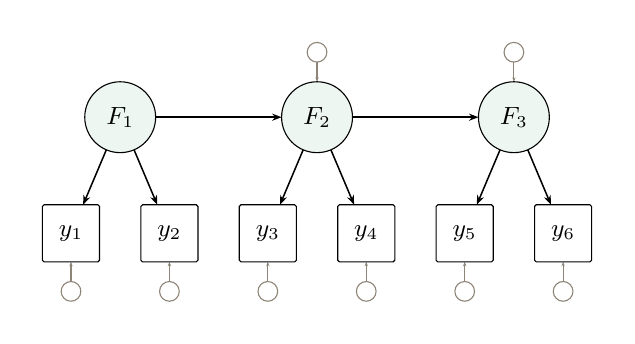
\begin{tikzpicture}[x=1cm, y=1cm,
    obs/.style={draw, rounded corners=0.6pt, minimum size=0.725cm, inner sep=0pt, fill=white, font=\fontsize{9.0}{10}\selectfont},
    lat/.style={draw, circle, minimum size=0.900cm, inner sep=0pt, fill=latfill, font=\fontsize{9.0}{10}\selectfont},
    resid/.style={draw=residc, line width=0.4pt}, residarrow/.style={draw=residc, -{Stealth[length=1.6pt]}, line width=0.4pt},
    path/.style={-{Stealth[length=3.4pt]}, line width=0.55pt},
    cov/.style={{Stealth[length=3.4pt]}-{Stealth[length=3.4pt]}, line width=0.55pt},
    net/.style={draw=netc, line width=1.1pt, line cap=round},
    elabel/.style={font=\scriptsize\itshape, fill=white, inner sep=0.6pt}]
\useasboundingbox (-0.550,-0.263) rectangle (6.800,-3.925);
\draw[resid] (0.000,-3.612) circle (0.125);
\draw[residarrow] (0.000,-3.487) -- (0.000,-3.237);
\draw[resid] (1.250,-3.612) circle (0.125);
\draw[residarrow] (1.250,-3.487) -- (1.250,-3.237);
\draw[resid] (2.500,-3.612) circle (0.125);
\draw[residarrow] (2.500,-3.487) -- (2.500,-3.237);
\draw[resid] (3.750,-3.612) circle (0.125);
\draw[residarrow] (3.750,-3.487) -- (3.750,-3.237);
\draw[resid] (5.000,-3.612) circle (0.125);
\draw[residarrow] (5.000,-3.487) -- (5.000,-3.237);
\draw[resid] (6.250,-3.612) circle (0.125);
\draw[residarrow] (6.250,-3.487) -- (6.250,-3.237);
\draw[resid] (3.125,-0.575) circle (0.125);
\draw[residarrow] (3.125,-0.700) -- (3.125,-0.950);
\draw[resid] (5.625,-0.575) circle (0.125);
\draw[residarrow] (5.625,-0.700) -- (5.625,-0.950);
\draw[path] (0.449,-1.814) -- (0.154,-2.512);
\draw[path] (0.801,-1.814) -- (1.096,-2.512);
\draw[path] (2.949,-1.814) -- (2.654,-2.512);
\draw[path] (3.301,-1.814) -- (3.596,-2.512);
\draw[path] (5.449,-1.814) -- (5.154,-2.512);
\draw[path] (5.801,-1.814) -- (6.096,-2.512);
\draw[path] (1.075,-1.400) -- (2.675,-1.400);
\draw[path] (3.575,-1.400) -- (5.175,-1.400);
\node[obs] at (0.000,-2.875) {$y_{1}$};
\node[obs] at (1.250,-2.875) {$y_{2}$};
\node[obs] at (2.500,-2.875) {$y_{3}$};
\node[obs] at (3.750,-2.875) {$y_{4}$};
\node[obs] at (5.000,-2.875) {$y_{5}$};
\node[obs] at (6.250,-2.875) {$y_{6}$};
\node[lat] at (0.625,-1.400) {$F_{1}$};
\node[lat] at (3.125,-1.400) {$F_{2}$};
\node[lat] at (5.625,-1.400) {$F_{3}$};
\end{tikzpicture}\\[1pt]{\scriptsize \texttt{F1 =\char`\~{} y1 + y2; F2 =\char`\~{} y3 + y4; F3 =\char`\~{} y5 + y6; F2 \char`\~{} F1; F3 \char`\~{} F2}}\end{minipage}\hfill
\begin{minipage}[t]{0.49\textwidth}\centering\textbf{\color{bcol}Model B} \;{\small $q_B=14$}\\[2pt]
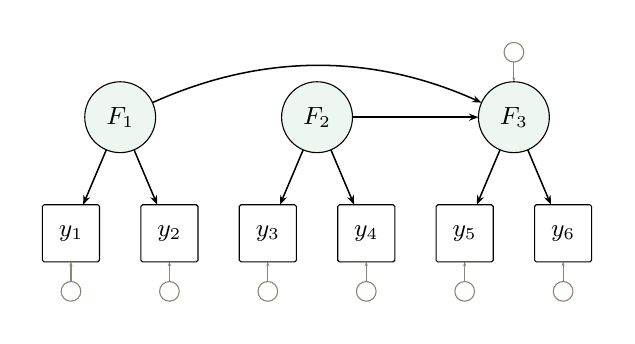
\begin{tikzpicture}[x=1cm, y=1cm,
    obs/.style={draw, rounded corners=0.6pt, minimum size=0.725cm, inner sep=0pt, fill=white, font=\fontsize{9.0}{10}\selectfont},
    lat/.style={draw, circle, minimum size=0.900cm, inner sep=0pt, fill=latfill, font=\fontsize{9.0}{10}\selectfont},
    resid/.style={draw=residc, line width=0.4pt}, residarrow/.style={draw=residc, -{Stealth[length=1.6pt]}, line width=0.4pt},
    path/.style={-{Stealth[length=3.4pt]}, line width=0.55pt},
    cov/.style={{Stealth[length=3.4pt]}-{Stealth[length=3.4pt]}, line width=0.55pt},
    net/.style={draw=netc, line width=1.1pt, line cap=round},
    elabel/.style={font=\scriptsize\itshape, fill=white, inner sep=0.6pt}]
\useasboundingbox (-0.550,-0.263) rectangle (6.800,-3.925);
\draw[resid] (0.000,-3.612) circle (0.125);
\draw[residarrow] (0.000,-3.487) -- (0.000,-3.237);
\draw[resid] (1.250,-3.612) circle (0.125);
\draw[residarrow] (1.250,-3.487) -- (1.250,-3.237);
\draw[resid] (2.500,-3.612) circle (0.125);
\draw[residarrow] (2.500,-3.487) -- (2.500,-3.237);
\draw[resid] (3.750,-3.612) circle (0.125);
\draw[residarrow] (3.750,-3.487) -- (3.750,-3.237);
\draw[resid] (5.000,-3.612) circle (0.125);
\draw[residarrow] (5.000,-3.487) -- (5.000,-3.237);
\draw[resid] (6.250,-3.612) circle (0.125);
\draw[residarrow] (6.250,-3.487) -- (6.250,-3.237);
\draw[resid] (5.625,-0.575) circle (0.125);
\draw[residarrow] (5.625,-0.700) -- (5.625,-0.950);
\draw[path] (0.449,-1.814) -- (0.154,-2.512);
\draw[path] (0.801,-1.814) -- (1.096,-2.512);
\draw[path] (2.949,-1.814) -- (2.654,-2.512);
\draw[path] (3.301,-1.814) -- (3.596,-2.512);
\draw[path] (5.449,-1.814) -- (5.154,-2.512);
\draw[path] (5.801,-1.814) -- (6.096,-2.512);
\draw[path] (1.035,-1.215) .. controls (2.428,-0.588) and (3.822,-0.588) .. (5.215,-1.215);
\draw[path] (3.575,-1.400) -- (5.175,-1.400);
\node[obs] at (0.000,-2.875) {$y_{1}$};
\node[obs] at (1.250,-2.875) {$y_{2}$};
\node[obs] at (2.500,-2.875) {$y_{3}$};
\node[obs] at (3.750,-2.875) {$y_{4}$};
\node[obs] at (5.000,-2.875) {$y_{5}$};
\node[obs] at (6.250,-2.875) {$y_{6}$};
\node[lat] at (0.625,-1.400) {$F_{1}$};
\node[lat] at (3.125,-1.400) {$F_{2}$};
\node[lat] at (5.625,-1.400) {$F_{3}$};
\end{tikzpicture}\\[1pt]{\scriptsize \texttt{F1 =\char`\~{} y1 + y2; F2 =\char`\~{} y3 + y4; F3 =\char`\~{} y5 + y6; F3 \char`\~{} F1 + F2}}\end{minipage}
\par\bigskip
\noindent\textbf{Claim.} $A \nnest B$ and $B \nnest A$: \textbf{neither} is nested in the other.\par\smallskip
\noindent\textbf{Proof.} (i) $A\nnest B$ by Lemma~S with $f(\Sigma)=\sigma_{13}$. In $B$, $F_1$ and $F_2$ are exogenous and uncorrelated, so indicators of $F_1$ and $F_2$ are uncorrelated. So $f\equiv0$ on $\mathcal M_B$, whereas in model $A$, $f=\lambda_1\lambda_3\psi_{12}\neq0$ for generic parameters; e.g.\ at the point of Appendix~B, $f=0.5000\neq0$.\par\smallskip
\noindent(ii) $B\nnest A$ by Lemma~S with $f(\Sigma)=\sigma_{15}\sigma_{34} - \sigma_{13}\sigma_{45}$. In $A$ this equals $\lambda_1\lambda_3\lambda_4\lambda_5(\psi_{13}\psi_{22}-\psi_{12}\psi_{23})$, and the chain implies $\psi_{13}\psi_{22}=\psi_{12}\psi_{23}$. So $f\equiv0$ on $\mathcal M_A$, whereas in model $B$ at the point of Appendix~B, $f=0.5400\neq0$.\hfill$\square$\par\medskip
\noindent{\small\textit{In the game:} A chain (F1 and F3 independent given F2) against a collider (F1 and F2 independent). Each model has a restriction the other violates.}

\clearpage
\section*{M01 \quad Residual covariance versus a second factor}
\addcontentsline{toc}{subsection}{M01\quad Residual covariance versus a second factor}
\noindent\textit{Level: Medium.} Observed variables: $y_{1}, y_{2}, y_{3}, y_{4}$ ($p=4$, 10 moments).\par\medskip
\noindent\begin{minipage}[t]{0.49\textwidth}\centering\textbf{\color{acol}Model A} \;{\small $q_A=9$}\\[2pt]
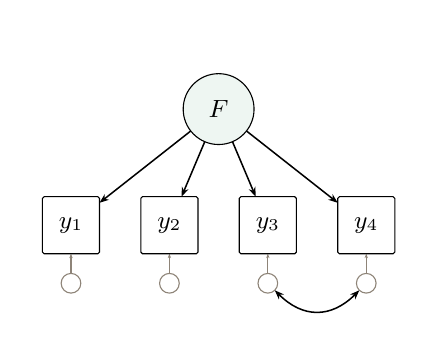
\begin{tikzpicture}[x=1cm, y=1cm,
    obs/.style={draw, rounded corners=0.6pt, minimum size=0.725cm, inner sep=0pt, fill=white, font=\fontsize{9.0}{10}\selectfont},
    lat/.style={draw, circle, minimum size=0.900cm, inner sep=0pt, fill=latfill, font=\fontsize{9.0}{10}\selectfont},
    resid/.style={draw=residc, line width=0.4pt}, residarrow/.style={draw=residc, -{Stealth[length=1.6pt]}, line width=0.4pt},
    path/.style={-{Stealth[length=3.4pt]}, line width=0.55pt},
    cov/.style={{Stealth[length=3.4pt]}-{Stealth[length=3.4pt]}, line width=0.55pt},
    net/.style={draw=netc, line width=1.1pt, line cap=round},
    elabel/.style={font=\scriptsize\itshape, fill=white, inner sep=0.6pt}]
\useasboundingbox (-0.550,-0.366) rectangle (4.300,-4.219);
\draw[resid] (0.000,-3.612) circle (0.125);
\draw[residarrow] (0.000,-3.487) -- (0.000,-3.237);
\draw[resid] (1.250,-3.612) circle (0.125);
\draw[residarrow] (1.250,-3.487) -- (1.250,-3.237);
\draw[resid] (2.500,-3.612) circle (0.125);
\draw[residarrow] (2.500,-3.487) -- (2.500,-3.237);
\draw[resid] (3.750,-3.612) circle (0.125);
\draw[residarrow] (3.750,-3.487) -- (3.750,-3.237);
\draw[path] (1.521,-1.678) -- (0.362,-2.590);
\draw[path] (1.699,-1.814) -- (1.404,-2.512);
\draw[path] (2.051,-1.814) -- (2.346,-2.512);
\draw[path] (2.229,-1.678) -- (3.388,-2.590);
\draw[cov] (2.588,-3.701) .. controls (2.946,-4.059) and (3.304,-4.059) .. (3.662,-3.701);
\node[obs] at (0.000,-2.875) {$y_{1}$};
\node[obs] at (1.250,-2.875) {$y_{2}$};
\node[obs] at (2.500,-2.875) {$y_{3}$};
\node[obs] at (3.750,-2.875) {$y_{4}$};
\node[lat] at (1.875,-1.400) {$F$};
\end{tikzpicture}\\[1pt]{\scriptsize \texttt{F =\char`\~{} y1 + y2 + y3 + y4; y3 \char`\~{}\char`\~{} y4}}\end{minipage}\hfill
\begin{minipage}[t]{0.49\textwidth}\centering\textbf{\color{bcol}Model B} \;{\small $q_B=9$}\\[2pt]
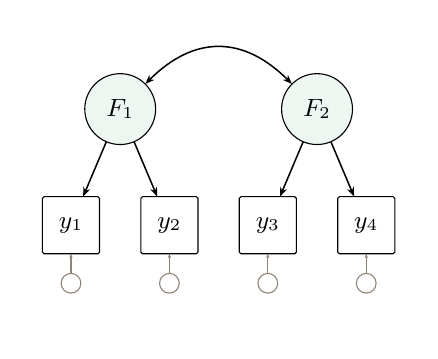
\begin{tikzpicture}[x=1cm, y=1cm,
    obs/.style={draw, rounded corners=0.6pt, minimum size=0.725cm, inner sep=0pt, fill=white, font=\fontsize{9.0}{10}\selectfont},
    lat/.style={draw, circle, minimum size=0.900cm, inner sep=0pt, fill=latfill, font=\fontsize{9.0}{10}\selectfont},
    resid/.style={draw=residc, line width=0.4pt}, residarrow/.style={draw=residc, -{Stealth[length=1.6pt]}, line width=0.4pt},
    path/.style={-{Stealth[length=3.4pt]}, line width=0.55pt},
    cov/.style={{Stealth[length=3.4pt]}-{Stealth[length=3.4pt]}, line width=0.55pt},
    net/.style={draw=netc, line width=1.1pt, line cap=round},
    elabel/.style={font=\scriptsize\itshape, fill=white, inner sep=0.6pt}]
\useasboundingbox (-0.550,-0.366) rectangle (4.300,-4.219);
\draw[resid] (0.000,-3.612) circle (0.125);
\draw[residarrow] (0.000,-3.487) -- (0.000,-3.237);
\draw[resid] (1.250,-3.612) circle (0.125);
\draw[residarrow] (1.250,-3.487) -- (1.250,-3.237);
\draw[resid] (2.500,-3.612) circle (0.125);
\draw[residarrow] (2.500,-3.487) -- (2.500,-3.237);
\draw[resid] (3.750,-3.612) circle (0.125);
\draw[residarrow] (3.750,-3.487) -- (3.750,-3.237);
\draw[path] (0.449,-1.814) -- (0.154,-2.512);
\draw[path] (0.801,-1.814) -- (1.096,-2.512);
\draw[path] (2.949,-1.814) -- (2.654,-2.512);
\draw[path] (3.301,-1.814) -- (3.596,-2.512);
\draw[cov] (0.943,-1.082) .. controls (1.564,-0.461) and (2.186,-0.461) .. (2.807,-1.082);
\node[obs] at (0.000,-2.875) {$y_{1}$};
\node[obs] at (1.250,-2.875) {$y_{2}$};
\node[obs] at (2.500,-2.875) {$y_{3}$};
\node[obs] at (3.750,-2.875) {$y_{4}$};
\node[lat] at (0.625,-1.400) {$F_{1}$};
\node[lat] at (3.125,-1.400) {$F_{2}$};
\end{tikzpicture}\\[1pt]{\scriptsize \texttt{F1 =\char`\~{} y1 + y2; F2 =\char`\~{} y3 + y4; F1 \char`\~{}\char`\~{} F2}}\end{minipage}
\par\bigskip
\noindent\textbf{Claim.} $A \equiv B$: the models are \textbf{equivalent}.\par\smallskip
\noindent\textbf{Proof.} (i) $A\nest B$. Lemma~P with the pair $(y_3,y_4)$: $A\equiv F\{y_1,y_2\}\to G\{y_3,y_4\}$. The latent block $(F,G)$ is saturated in both that model and $B$ (Lemma~B(b), as in E03), so $A\equiv B$. Both equal $\{\Sigma\succ0:\sigma_{13}\sigma_{24}=\sigma_{14}\sigma_{23}\}$.\par\smallskip
\noindent(ii) $B\nest A$. See above.\hfill$\square$\par\medskip
\noindent{\small\textit{In the game:} Both models imply a single restriction, the tetrad σ13·σ24 = σ14·σ23, and nothing else (9 parameters each). The residual covariance does the same job as splitting off a second factor.}

\clearpage
\section*{M02 \quad Higher-order model with three first-order factors}
\addcontentsline{toc}{subsection}{M02\quad Higher-order model with three first-order factors}
\noindent\textit{Level: Medium.} Observed variables: $y_{1}, y_{2}, y_{3}, y_{4}, y_{5}, y_{6}, y_{7}, y_{8}, y_{9}$ ($p=9$, 45 moments).\par\medskip
\noindent\begin{minipage}[t]{0.49\textwidth}\centering\textbf{\color{acol}Model A} \;{\small $q_A=21$}\\[2pt]
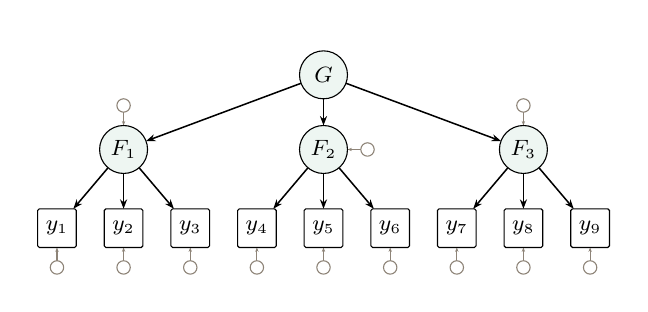
\begin{tikzpicture}[x=1cm, y=1cm,
    obs/.style={draw, rounded corners=0.6pt, minimum size=0.491cm, inner sep=0pt, fill=white, font=\fontsize{7.6}{10}\selectfont},
    lat/.style={draw, circle, minimum size=0.609cm, inner sep=0pt, fill=latfill, font=\fontsize{7.6}{10}\selectfont},
    resid/.style={draw=residc, line width=0.4pt}, residarrow/.style={draw=residc, -{Stealth[length=1.6pt]}, line width=0.4pt},
    path/.style={-{Stealth[length=3.4pt]}, line width=0.55pt},
    cov/.style={{Stealth[length=3.4pt]}-{Stealth[length=3.4pt]}, line width=0.55pt},
    net/.style={draw=netc, line width=1.1pt, line cap=round},
    elabel/.style={font=\scriptsize\itshape, fill=white, inner sep=0.6pt}]
\useasboundingbox (-0.372,0.599) rectangle (7.143,-2.657);
\draw[resid] (0.000,-2.446) circle (0.085);
\draw[residarrow] (0.000,-2.361) -- (0.000,-2.192);
\draw[resid] (0.846,-2.446) circle (0.085);
\draw[residarrow] (0.846,-2.361) -- (0.846,-2.192);
\draw[resid] (1.693,-2.446) circle (0.085);
\draw[residarrow] (1.693,-2.361) -- (1.693,-2.192);
\draw[resid] (2.539,-2.446) circle (0.085);
\draw[residarrow] (2.539,-2.361) -- (2.539,-2.192);
\draw[resid] (3.385,-2.446) circle (0.085);
\draw[residarrow] (3.385,-2.361) -- (3.385,-2.192);
\draw[resid] (4.232,-2.446) circle (0.085);
\draw[residarrow] (4.232,-2.361) -- (4.232,-2.192);
\draw[resid] (5.078,-2.446) circle (0.085);
\draw[residarrow] (5.078,-2.361) -- (5.078,-2.192);
\draw[resid] (5.924,-2.446) circle (0.085);
\draw[residarrow] (5.924,-2.361) -- (5.924,-2.192);
\draw[resid] (6.771,-2.446) circle (0.085);
\draw[residarrow] (6.771,-2.361) -- (6.771,-2.192);
\draw[resid] (0.846,-0.389) circle (0.085);
\draw[residarrow] (0.846,-0.474) -- (0.846,-0.643);
\draw[resid] (3.944,-0.948) circle (0.085);
\draw[residarrow] (3.859,-0.948) -- (3.690,-0.948);
\draw[resid] (5.924,-0.389) circle (0.085);
\draw[residarrow] (5.924,-0.474) -- (5.924,-0.643);
\draw[path] (0.649,-1.180) -- (0.208,-1.701);
\draw[path] (0.846,-1.253) -- (0.846,-1.701);
\draw[path] (1.043,-1.180) -- (1.485,-1.701);
\draw[path] (3.188,-1.180) -- (2.747,-1.701);
\draw[path] (3.385,-1.253) -- (3.385,-1.701);
\draw[path] (3.582,-1.180) -- (4.024,-1.701);
\draw[path] (5.727,-1.180) -- (5.286,-1.701);
\draw[path] (5.924,-1.253) -- (5.924,-1.701);
\draw[path] (6.121,-1.180) -- (6.563,-1.701);
\draw[path] (3.100,-0.107) -- (1.132,-0.841);
\draw[path] (3.385,-0.305) -- (3.385,-0.643);
\draw[path] (3.671,-0.107) -- (5.639,-0.841);
\node[obs] at (0.000,-1.947) {$y_{1}$};
\node[obs] at (0.846,-1.947) {$y_{2}$};
\node[obs] at (1.693,-1.947) {$y_{3}$};
\node[obs] at (2.539,-1.947) {$y_{4}$};
\node[obs] at (3.385,-1.947) {$y_{5}$};
\node[obs] at (4.232,-1.947) {$y_{6}$};
\node[obs] at (5.078,-1.947) {$y_{7}$};
\node[obs] at (5.924,-1.947) {$y_{8}$};
\node[obs] at (6.771,-1.947) {$y_{9}$};
\node[lat] at (0.846,-0.948) {$F_{1}$};
\node[lat] at (3.385,-0.948) {$F_{2}$};
\node[lat] at (5.924,-0.948) {$F_{3}$};
\node[lat] at (3.385,0.000) {$G$};
\end{tikzpicture}\\[1pt]{\scriptsize \texttt{F1 =\char`\~{} y1 + y2 + y3; F2 =\char`\~{} y4 + y5 + y6; F3 =\char`\~{} y7 + y8 + y9; G =\char`\~{} F1 + F2 + F3}}\end{minipage}\hfill
\begin{minipage}[t]{0.49\textwidth}\centering\textbf{\color{bcol}Model B} \;{\small $q_B=21$}\\[2pt]
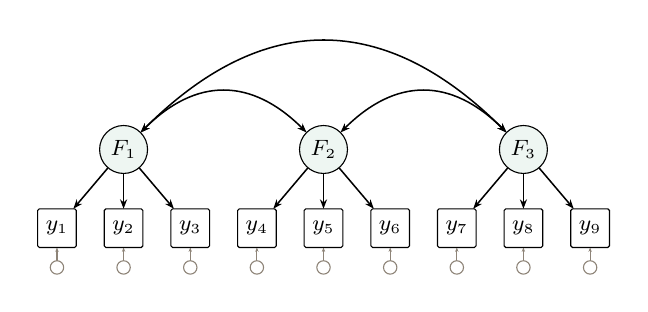
\begin{tikzpicture}[x=1cm, y=1cm,
    obs/.style={draw, rounded corners=0.6pt, minimum size=0.491cm, inner sep=0pt, fill=white, font=\fontsize{7.6}{10}\selectfont},
    lat/.style={draw, circle, minimum size=0.609cm, inner sep=0pt, fill=latfill, font=\fontsize{7.6}{10}\selectfont},
    resid/.style={draw=residc, line width=0.4pt}, residarrow/.style={draw=residc, -{Stealth[length=1.6pt]}, line width=0.4pt},
    path/.style={-{Stealth[length=3.4pt]}, line width=0.55pt},
    cov/.style={{Stealth[length=3.4pt]}-{Stealth[length=3.4pt]}, line width=0.55pt},
    net/.style={draw=netc, line width=1.1pt, line cap=round},
    elabel/.style={font=\scriptsize\itshape, fill=white, inner sep=0.6pt}]
\useasboundingbox (-0.372,0.599) rectangle (7.143,-2.657);
\draw[resid] (0.000,-2.446) circle (0.085);
\draw[residarrow] (0.000,-2.361) -- (0.000,-2.192);
\draw[resid] (0.846,-2.446) circle (0.085);
\draw[residarrow] (0.846,-2.361) -- (0.846,-2.192);
\draw[resid] (1.693,-2.446) circle (0.085);
\draw[residarrow] (1.693,-2.361) -- (1.693,-2.192);
\draw[resid] (2.539,-2.446) circle (0.085);
\draw[residarrow] (2.539,-2.361) -- (2.539,-2.192);
\draw[resid] (3.385,-2.446) circle (0.085);
\draw[residarrow] (3.385,-2.361) -- (3.385,-2.192);
\draw[resid] (4.232,-2.446) circle (0.085);
\draw[residarrow] (4.232,-2.361) -- (4.232,-2.192);
\draw[resid] (5.078,-2.446) circle (0.085);
\draw[residarrow] (5.078,-2.361) -- (5.078,-2.192);
\draw[resid] (5.924,-2.446) circle (0.085);
\draw[residarrow] (5.924,-2.361) -- (5.924,-2.192);
\draw[resid] (6.771,-2.446) circle (0.085);
\draw[residarrow] (6.771,-2.361) -- (6.771,-2.192);
\draw[path] (0.649,-1.180) -- (0.208,-1.701);
\draw[path] (0.846,-1.253) -- (0.846,-1.701);
\draw[path] (1.043,-1.180) -- (1.485,-1.701);
\draw[path] (3.188,-1.180) -- (2.747,-1.701);
\draw[path] (3.385,-1.253) -- (3.385,-1.701);
\draw[path] (3.582,-1.180) -- (4.024,-1.701);
\draw[path] (5.727,-1.180) -- (5.286,-1.701);
\draw[path] (5.924,-1.253) -- (5.924,-1.701);
\draw[path] (6.121,-1.180) -- (6.563,-1.701);
\draw[cov] (1.062,-0.732) .. controls (1.764,-0.030) and (2.467,-0.030) .. (3.170,-0.732);
\draw[cov] (1.062,-0.732) .. controls (2.611,0.817) and (4.160,0.817) .. (5.709,-0.732);
\draw[cov] (3.601,-0.732) .. controls (4.303,-0.030) and (5.006,-0.030) .. (5.709,-0.732);
\node[obs] at (0.000,-1.947) {$y_{1}$};
\node[obs] at (0.846,-1.947) {$y_{2}$};
\node[obs] at (1.693,-1.947) {$y_{3}$};
\node[obs] at (2.539,-1.947) {$y_{4}$};
\node[obs] at (3.385,-1.947) {$y_{5}$};
\node[obs] at (4.232,-1.947) {$y_{6}$};
\node[obs] at (5.078,-1.947) {$y_{7}$};
\node[obs] at (5.924,-1.947) {$y_{8}$};
\node[obs] at (6.771,-1.947) {$y_{9}$};
\node[lat] at (0.846,-0.948) {$F_{1}$};
\node[lat] at (3.385,-0.948) {$F_{2}$};
\node[lat] at (5.924,-0.948) {$F_{3}$};
\end{tikzpicture}\\[1pt]{\scriptsize \texttt{F1 =\char`\~{} y1 + y2 + y3; F2 =\char`\~{} y4 + y5 + y6; F3 =\char`\~{} y7 + y8 + y9; F1 \char`\~{}\char`\~{} F2 + F3; F2 \char`\~{}\char`\~{} F3}}\end{minipage}
\par\bigskip
\noindent\textbf{Claim.} $A \equiv B$: the models are \textbf{equivalent}.\par\smallskip
\noindent\textbf{Proof.} (i) $A\nest B$. Same measurement part. In $B$, $\Psi$ is free. In $A$, $\Psi=\gamma\gamma^\top\psi_G+\mathrm{diag}(\zeta)$ is a one-factor model on three variables, which by Lemma~B(a) reproduces every $\Psi$ with $\psi_{12}\psi_{13}\psi_{23}\neq0$. Lemmas~B(b) and G give $A\equiv B$.\par\smallskip
\noindent(ii) $B\nest A$. See above (with $\gamma_1=1$, $\psi_G=\psi_{12}\psi_{13}/\psi_{23}$, \dots).\hfill$\square$\par\medskip
\noindent{\small\textit{In the game:} A second-order factor on three first-order factors has three loadings for three factor covariances: it is just-identified, so it reproduces any correlation pattern among three factors.}

\clearpage
\section*{M03 \quad A two-indicator factor}
\addcontentsline{toc}{subsection}{M03\quad A two-indicator factor}
\noindent\textit{Level: Medium.} Observed variables: $y_{1}, y_{2}, y_{3}, y_{4}, y_{5}$ ($p=5$, 15 moments).\par\medskip
\noindent\begin{minipage}[t]{0.49\textwidth}\centering\textbf{\color{acol}Model A} \;{\small $q_A=11$}\\[2pt]
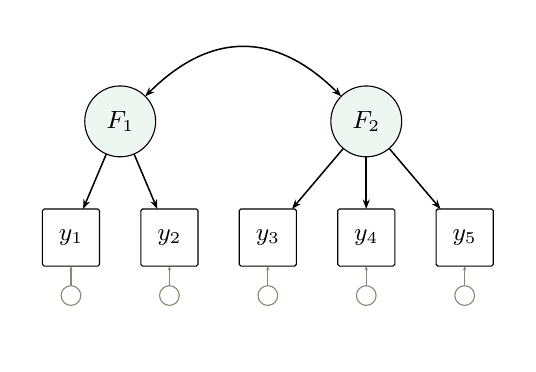
\begin{tikzpicture}[x=1cm, y=1cm,
    obs/.style={draw, rounded corners=0.6pt, minimum size=0.725cm, inner sep=0pt, fill=white, font=\fontsize{9.0}{10}\selectfont},
    lat/.style={draw, circle, minimum size=0.900cm, inner sep=0pt, fill=latfill, font=\fontsize{9.0}{10}\selectfont},
    resid/.style={draw=residc, line width=0.4pt}, residarrow/.style={draw=residc, -{Stealth[length=1.6pt]}, line width=0.4pt},
    path/.style={-{Stealth[length=3.4pt]}, line width=0.55pt},
    cov/.style={{Stealth[length=3.4pt]}-{Stealth[length=3.4pt]}, line width=0.55pt},
    net/.style={draw=netc, line width=1.1pt, line cap=round},
    elabel/.style={font=\scriptsize\itshape, fill=white, inner sep=0.6pt}]
\useasboundingbox (-0.550,-0.210) rectangle (5.550,-4.219);
\draw[resid] (0.000,-3.612) circle (0.125);
\draw[residarrow] (0.000,-3.487) -- (0.000,-3.237);
\draw[resid] (1.250,-3.612) circle (0.125);
\draw[residarrow] (1.250,-3.487) -- (1.250,-3.237);
\draw[resid] (2.500,-3.612) circle (0.125);
\draw[residarrow] (2.500,-3.487) -- (2.500,-3.237);
\draw[resid] (3.750,-3.612) circle (0.125);
\draw[residarrow] (3.750,-3.487) -- (3.750,-3.237);
\draw[resid] (5.000,-3.612) circle (0.125);
\draw[residarrow] (5.000,-3.487) -- (5.000,-3.237);
\draw[path] (0.449,-1.814) -- (0.154,-2.512);
\draw[path] (0.801,-1.814) -- (1.096,-2.512);
\draw[path] (3.459,-1.743) -- (2.807,-2.512);
\draw[path] (3.750,-1.850) -- (3.750,-2.512);
\draw[path] (4.041,-1.743) -- (4.693,-2.512);
\draw[cov] (0.943,-1.082) .. controls (1.773,-0.252) and (2.602,-0.252) .. (3.432,-1.082);
\node[obs] at (0.000,-2.875) {$y_{1}$};
\node[obs] at (1.250,-2.875) {$y_{2}$};
\node[obs] at (2.500,-2.875) {$y_{3}$};
\node[obs] at (3.750,-2.875) {$y_{4}$};
\node[obs] at (5.000,-2.875) {$y_{5}$};
\node[lat] at (0.625,-1.400) {$F_{1}$};
\node[lat] at (3.750,-1.400) {$F_{2}$};
\end{tikzpicture}\\[1pt]{\scriptsize \texttt{F1 =\char`\~{} y1 + y2; F2 =\char`\~{} y3 + y4 + y5; F1 \char`\~{}\char`\~{} F2}}\end{minipage}\hfill
\begin{minipage}[t]{0.49\textwidth}\centering\textbf{\color{bcol}Model B} \;{\small $q_B=11$}\\[2pt]
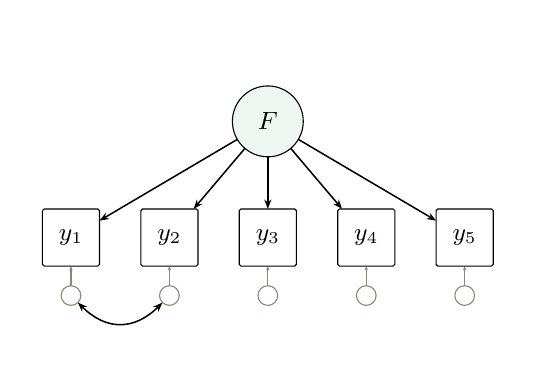
\begin{tikzpicture}[x=1cm, y=1cm,
    obs/.style={draw, rounded corners=0.6pt, minimum size=0.725cm, inner sep=0pt, fill=white, font=\fontsize{9.0}{10}\selectfont},
    lat/.style={draw, circle, minimum size=0.900cm, inner sep=0pt, fill=latfill, font=\fontsize{9.0}{10}\selectfont},
    resid/.style={draw=residc, line width=0.4pt}, residarrow/.style={draw=residc, -{Stealth[length=1.6pt]}, line width=0.4pt},
    path/.style={-{Stealth[length=3.4pt]}, line width=0.55pt},
    cov/.style={{Stealth[length=3.4pt]}-{Stealth[length=3.4pt]}, line width=0.55pt},
    net/.style={draw=netc, line width=1.1pt, line cap=round},
    elabel/.style={font=\scriptsize\itshape, fill=white, inner sep=0.6pt}]
\useasboundingbox (-0.550,-0.210) rectangle (5.550,-4.219);
\draw[resid] (0.000,-3.612) circle (0.125);
\draw[residarrow] (0.000,-3.487) -- (0.000,-3.237);
\draw[resid] (1.250,-3.612) circle (0.125);
\draw[residarrow] (1.250,-3.487) -- (1.250,-3.237);
\draw[resid] (2.500,-3.612) circle (0.125);
\draw[residarrow] (2.500,-3.487) -- (2.500,-3.237);
\draw[resid] (3.750,-3.612) circle (0.125);
\draw[residarrow] (3.750,-3.487) -- (3.750,-3.237);
\draw[resid] (5.000,-3.612) circle (0.125);
\draw[residarrow] (5.000,-3.487) -- (5.000,-3.237);
\draw[path] (2.112,-1.629) -- (0.362,-2.661);
\draw[path] (2.209,-1.743) -- (1.557,-2.512);
\draw[path] (2.500,-1.850) -- (2.500,-2.512);
\draw[path] (2.791,-1.743) -- (3.443,-2.512);
\draw[path] (2.888,-1.629) -- (4.638,-2.661);
\draw[cov] (0.088,-3.701) .. controls (0.446,-4.059) and (0.804,-4.059) .. (1.162,-3.701);
\node[obs] at (0.000,-2.875) {$y_{1}$};
\node[obs] at (1.250,-2.875) {$y_{2}$};
\node[obs] at (2.500,-2.875) {$y_{3}$};
\node[obs] at (3.750,-2.875) {$y_{4}$};
\node[obs] at (5.000,-2.875) {$y_{5}$};
\node[lat] at (2.500,-1.400) {$F$};
\end{tikzpicture}\\[1pt]{\scriptsize \texttt{F =\char`\~{} y1 + y2 + y3 + y4 + y5; y1 \char`\~{}\char`\~{} y2}}\end{minipage}
\par\bigskip
\noindent\textbf{Claim.} $A \equiv B$: the models are \textbf{equivalent}.\par\smallskip
\noindent\textbf{Proof.} (i) $A\nest B$. $A$ has a factor $F_1$ with only $y_1,y_2$ and a free covariance with $F_2$. By Lemma~P (pair $(y_1,y_2)$), $B\equiv F\{y_3,y_4,y_5\}\to G\{y_1,y_2\}$, and $F\to G$ and $F\leftrightarrow G$ give the same (saturated) $2\times2$ latent block (Lemma~B(b)).\par\smallskip
\noindent(ii) $B\nest A$. See above.\hfill$\square$\par\medskip
\noindent{\small\textit{In the game:} A factor with only two indicators adds exactly one free covariance (between those two items) on top of a single common factor. That is what the residual covariance y1 ↔ y2 does in B.}

\clearpage
\section*{M04 \quad The replacing rule}
\addcontentsline{toc}{subsection}{M04\quad The replacing rule}
\noindent\textit{Level: Medium.} Observed variables: $A, B, C, D$ ($p=4$, 10 moments).\par\medskip
\noindent\begin{minipage}[t]{0.49\textwidth}\centering\textbf{\color{acol}Model A} \;{\small $q_A=9$}\\[2pt]
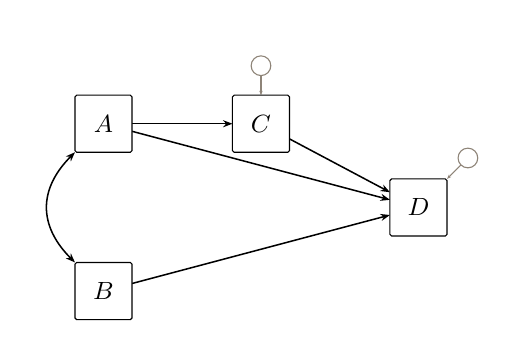
\begin{tikzpicture}[x=1cm, y=1cm,
    obs/.style={draw, rounded corners=0.6pt, minimum size=0.725cm, inner sep=0pt, fill=white, font=\fontsize{9.0}{10}\selectfont},
    lat/.style={draw, circle, minimum size=0.900cm, inner sep=0pt, fill=latfill, font=\fontsize{9.0}{10}\selectfont},
    resid/.style={draw=residc, line width=0.4pt}, residarrow/.style={draw=residc, -{Stealth[length=1.6pt]}, line width=0.4pt},
    path/.style={-{Stealth[length=3.4pt]}, line width=0.55pt},
    cov/.style={{Stealth[length=3.4pt]}-{Stealth[length=3.4pt]}, line width=0.55pt},
    net/.style={draw=netc, line width=1.1pt, line cap=round},
    elabel/.style={font=\scriptsize\itshape, fill=white, inner sep=0.6pt}]
\useasboundingbox (-0.963,1.220) rectangle (4.940,-2.675);
\draw[resid] (2.000,0.737) circle (0.125);
\draw[residarrow] (2.000,0.613) -- (2.000,0.362);
\draw[resid] (4.628,-0.435) circle (0.125);
\draw[residarrow] (4.539,-0.523) -- (4.363,-0.700);
\draw[path] (0.362,0.000) -- (1.638,0.000);
\draw[path] (2.363,-0.193) -- (3.638,-0.870);
\draw[path] (0.362,-0.096) -- (3.638,-0.966);
\draw[path] (0.362,-2.029) -- (3.638,-1.159);
\draw[cov] (-0.362,-0.362) .. controls (-0.829,-0.829) and (-0.829,-1.296) .. (-0.362,-1.762);
\node[obs] at (0.000,0.000) {$A$};
\node[obs] at (0.000,-2.125) {$B$};
\node[obs] at (2.000,0.000) {$C$};
\node[obs] at (4.000,-1.063) {$D$};
\end{tikzpicture}\\[1pt]{\scriptsize \texttt{A \char`\~{}\char`\~{} B; C \char`\~{} A; D \char`\~{} C + A + B}}\end{minipage}\hfill
\begin{minipage}[t]{0.49\textwidth}\centering\textbf{\color{bcol}Model B} \;{\small $q_B=9$}\\[2pt]
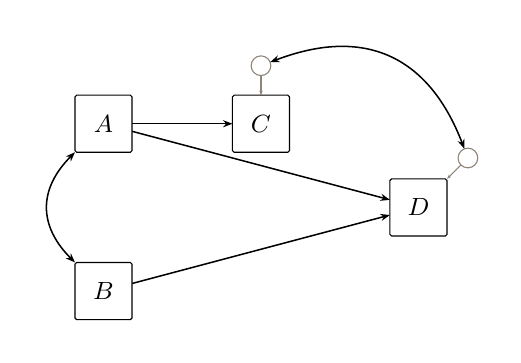
\begin{tikzpicture}[x=1cm, y=1cm,
    obs/.style={draw, rounded corners=0.6pt, minimum size=0.725cm, inner sep=0pt, fill=white, font=\fontsize{9.0}{10}\selectfont},
    lat/.style={draw, circle, minimum size=0.900cm, inner sep=0pt, fill=latfill, font=\fontsize{9.0}{10}\selectfont},
    resid/.style={draw=residc, line width=0.4pt}, residarrow/.style={draw=residc, -{Stealth[length=1.6pt]}, line width=0.4pt},
    path/.style={-{Stealth[length=3.4pt]}, line width=0.55pt},
    cov/.style={{Stealth[length=3.4pt]}-{Stealth[length=3.4pt]}, line width=0.55pt},
    net/.style={draw=netc, line width=1.1pt, line cap=round},
    elabel/.style={font=\scriptsize\itshape, fill=white, inner sep=0.6pt}]
\useasboundingbox (-0.963,1.220) rectangle (4.940,-2.675);
\draw[resid] (2.000,0.737) circle (0.125);
\draw[residarrow] (2.000,0.613) -- (2.000,0.362);
\draw[resid] (4.628,-0.435) circle (0.125);
\draw[residarrow] (4.539,-0.523) -- (4.363,-0.700);
\draw[path] (0.362,0.000) -- (1.638,0.000);
\draw[path] (0.362,-0.096) -- (3.638,-0.966);
\draw[path] (0.362,-2.029) -- (3.638,-1.159);
\draw[cov] (-0.362,-0.362) .. controls (-0.829,-0.829) and (-0.829,-1.296) .. (-0.362,-1.762);
\draw[cov] (2.117,0.782) .. controls (3.306,1.238) and (4.128,0.871) .. (4.583,-0.318);
\node[obs] at (0.000,0.000) {$A$};
\node[obs] at (0.000,-2.125) {$B$};
\node[obs] at (2.000,0.000) {$C$};
\node[obs] at (4.000,-1.063) {$D$};
\end{tikzpicture}\\[1pt]{\scriptsize \texttt{A \char`\~{}\char`\~{} B; C \char`\~{} A; D \char`\~{} A + B; C \char`\~{}\char`\~{} D}}\end{minipage}
\par\bigskip
\noindent\textbf{Claim.} $A \equiv B$: the models are \textbf{equivalent}.\par\smallskip
\noindent\textbf{Proof.} (i) $A\nest B$. Substitute $C=\beta_{CA}A+\zeta_C$ in $D$'s equation of $A$: $D=(\beta_{DA}+\beta_{DC}\beta_{CA})A+\beta_{DB}B+(\beta_{DC}\zeta_C+\zeta_D)$. This is model $B$ with residual $\zeta_D'=\beta_{DC}\zeta_C+\zeta_D$, $\mathrm{Var}(\zeta_D')=\beta_{DC}^2\psi_C+\psi_D$ and $\mathrm{Cov}(\zeta_C,\zeta_D')=\beta_{DC}\psi_C$.\par\smallskip
\noindent(ii) $B\nest A$. Conversely, for $\psi_C\neq0$ set $\beta_{DC}=\omega/\psi_C$ ($\omega=\mathrm{Cov}(\zeta_C,\zeta_D')$), $\beta_{DA}=\beta'_{DA}-\beta_{DC}\beta_{CA}$, $\psi_D=\psi'_D-\omega^2/\psi_C$ (Lemma~G).\hfill$\square$\par\medskip
\noindent{\small\textit{In the game:} Replacing rule (Lee \& Hershberger): C → D may be replaced by a residual covariance C ↔ D because the predictors of D include all predictors of C. Both models only claim that C and B are independent given A.}

\clearpage
\section*{M05 \quad A saturated structural block}
\addcontentsline{toc}{subsection}{M05\quad A saturated structural block}
\noindent\textit{Level: Medium.} Observed variables: $y_{1}, y_{2}, y_{3}, y_{4}, y_{5}, y_{6}$ ($p=6$, 21 moments).\par\medskip
\noindent\begin{minipage}[t]{0.49\textwidth}\centering\textbf{\color{acol}Model A} \;{\small $q_A=15$}\\[2pt]
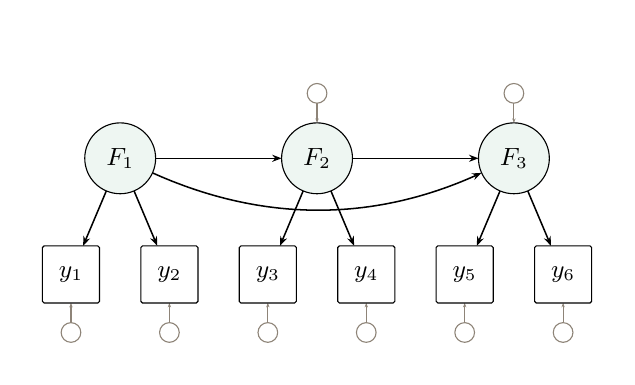
\begin{tikzpicture}[x=1cm, y=1cm,
    obs/.style={draw, rounded corners=0.6pt, minimum size=0.725cm, inner sep=0pt, fill=white, font=\fontsize{9.0}{10}\selectfont},
    lat/.style={draw, circle, minimum size=0.900cm, inner sep=0pt, fill=latfill, font=\fontsize{9.0}{10}\selectfont},
    resid/.style={draw=residc, line width=0.4pt}, residarrow/.style={draw=residc, -{Stealth[length=1.6pt]}, line width=0.4pt},
    path/.style={-{Stealth[length=3.4pt]}, line width=0.55pt},
    cov/.style={{Stealth[length=3.4pt]}-{Stealth[length=3.4pt]}, line width=0.55pt},
    net/.style={draw=netc, line width=1.1pt, line cap=round},
    elabel/.style={font=\scriptsize\itshape, fill=white, inner sep=0.6pt}]
\useasboundingbox (-0.550,0.259) rectangle (6.800,-3.925);
\draw[resid] (0.000,-3.612) circle (0.125);
\draw[residarrow] (0.000,-3.487) -- (0.000,-3.237);
\draw[resid] (1.250,-3.612) circle (0.125);
\draw[residarrow] (1.250,-3.487) -- (1.250,-3.237);
\draw[resid] (2.500,-3.612) circle (0.125);
\draw[residarrow] (2.500,-3.487) -- (2.500,-3.237);
\draw[resid] (3.750,-3.612) circle (0.125);
\draw[residarrow] (3.750,-3.487) -- (3.750,-3.237);
\draw[resid] (5.000,-3.612) circle (0.125);
\draw[residarrow] (5.000,-3.487) -- (5.000,-3.237);
\draw[resid] (6.250,-3.612) circle (0.125);
\draw[residarrow] (6.250,-3.487) -- (6.250,-3.237);
\draw[resid] (3.125,-0.575) circle (0.125);
\draw[residarrow] (3.125,-0.700) -- (3.125,-0.950);
\draw[resid] (5.625,-0.575) circle (0.125);
\draw[residarrow] (5.625,-0.700) -- (5.625,-0.950);
\draw[path] (0.449,-1.814) -- (0.154,-2.512);
\draw[path] (0.801,-1.814) -- (1.096,-2.512);
\draw[path] (2.949,-1.814) -- (2.654,-2.512);
\draw[path] (3.301,-1.814) -- (3.596,-2.512);
\draw[path] (5.449,-1.814) -- (5.154,-2.512);
\draw[path] (5.801,-1.814) -- (6.096,-2.512);
\draw[path] (1.075,-1.400) -- (2.675,-1.400);
\draw[path] (1.035,-1.585) .. controls (2.428,-2.212) and (3.822,-2.212) .. (5.215,-1.585);
\draw[path] (3.575,-1.400) -- (5.175,-1.400);
\node[obs] at (0.000,-2.875) {$y_{1}$};
\node[obs] at (1.250,-2.875) {$y_{2}$};
\node[obs] at (2.500,-2.875) {$y_{3}$};
\node[obs] at (3.750,-2.875) {$y_{4}$};
\node[obs] at (5.000,-2.875) {$y_{5}$};
\node[obs] at (6.250,-2.875) {$y_{6}$};
\node[lat] at (0.625,-1.400) {$F_{1}$};
\node[lat] at (3.125,-1.400) {$F_{2}$};
\node[lat] at (5.625,-1.400) {$F_{3}$};
\end{tikzpicture}\\[1pt]{\scriptsize \texttt{F1 =\char`\~{} y1 + y2; F2 =\char`\~{} y3 + y4; F3 =\char`\~{} y5 + y6; F2 \char`\~{} F1; F3 \char`\~{} F1 + F2}}\end{minipage}\hfill
\begin{minipage}[t]{0.49\textwidth}\centering\textbf{\color{bcol}Model B} \;{\small $q_B=15$}\\[2pt]
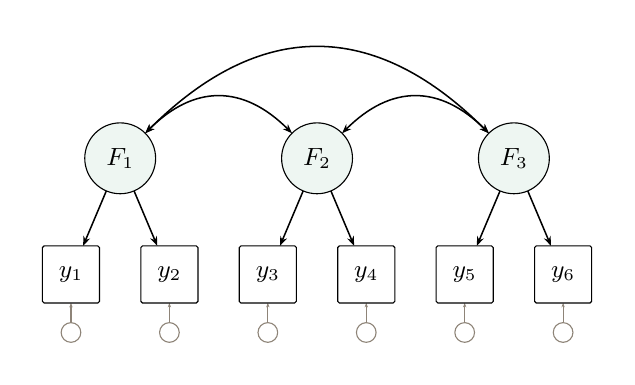
\begin{tikzpicture}[x=1cm, y=1cm,
    obs/.style={draw, rounded corners=0.6pt, minimum size=0.725cm, inner sep=0pt, fill=white, font=\fontsize{9.0}{10}\selectfont},
    lat/.style={draw, circle, minimum size=0.900cm, inner sep=0pt, fill=latfill, font=\fontsize{9.0}{10}\selectfont},
    resid/.style={draw=residc, line width=0.4pt}, residarrow/.style={draw=residc, -{Stealth[length=1.6pt]}, line width=0.4pt},
    path/.style={-{Stealth[length=3.4pt]}, line width=0.55pt},
    cov/.style={{Stealth[length=3.4pt]}-{Stealth[length=3.4pt]}, line width=0.55pt},
    net/.style={draw=netc, line width=1.1pt, line cap=round},
    elabel/.style={font=\scriptsize\itshape, fill=white, inner sep=0.6pt}]
\useasboundingbox (-0.550,0.259) rectangle (6.800,-3.925);
\draw[resid] (0.000,-3.612) circle (0.125);
\draw[residarrow] (0.000,-3.487) -- (0.000,-3.237);
\draw[resid] (1.250,-3.612) circle (0.125);
\draw[residarrow] (1.250,-3.487) -- (1.250,-3.237);
\draw[resid] (2.500,-3.612) circle (0.125);
\draw[residarrow] (2.500,-3.487) -- (2.500,-3.237);
\draw[resid] (3.750,-3.612) circle (0.125);
\draw[residarrow] (3.750,-3.487) -- (3.750,-3.237);
\draw[resid] (5.000,-3.612) circle (0.125);
\draw[residarrow] (5.000,-3.487) -- (5.000,-3.237);
\draw[resid] (6.250,-3.612) circle (0.125);
\draw[residarrow] (6.250,-3.487) -- (6.250,-3.237);
\draw[path] (0.449,-1.814) -- (0.154,-2.512);
\draw[path] (0.801,-1.814) -- (1.096,-2.512);
\draw[path] (2.949,-1.814) -- (2.654,-2.512);
\draw[path] (3.301,-1.814) -- (3.596,-2.512);
\draw[path] (5.449,-1.814) -- (5.154,-2.512);
\draw[path] (5.801,-1.814) -- (6.096,-2.512);
\draw[cov] (0.943,-1.082) .. controls (1.564,-0.461) and (2.186,-0.461) .. (2.807,-1.082);
\draw[cov] (0.943,-1.082) .. controls (2.398,0.373) and (3.852,0.373) .. (5.307,-1.082);
\draw[cov] (3.443,-1.082) .. controls (4.064,-0.461) and (4.686,-0.461) .. (5.307,-1.082);
\node[obs] at (0.000,-2.875) {$y_{1}$};
\node[obs] at (1.250,-2.875) {$y_{2}$};
\node[obs] at (2.500,-2.875) {$y_{3}$};
\node[obs] at (3.750,-2.875) {$y_{4}$};
\node[obs] at (5.000,-2.875) {$y_{5}$};
\node[obs] at (6.250,-2.875) {$y_{6}$};
\node[lat] at (0.625,-1.400) {$F_{1}$};
\node[lat] at (3.125,-1.400) {$F_{2}$};
\node[lat] at (5.625,-1.400) {$F_{3}$};
\end{tikzpicture}\\[1pt]{\scriptsize \texttt{F1 =\char`\~{} y1 + y2; F2 =\char`\~{} y3 + y4; F3 =\char`\~{} y5 + y6; F1 \char`\~{}\char`\~{} F2 + F3; F2 \char`\~{}\char`\~{} F3}}\end{minipage}
\par\bigskip
\noindent\textbf{Claim.} $A \equiv B$: the models are \textbf{equivalent}.\par\smallskip
\noindent\textbf{Proof.} (i) $A\nest B$. The structural part of $A$ is a complete recursive model on $(F_1,F_2,F_3)$, which reproduces every $\Psi\succ0$ (Cholesky, Lemma~B(a)); in $B$, $\Psi$ is free. Lemma~B(b).\par\smallskip
\noindent(ii) $B\nest A$. See above.\hfill$\square$\par\medskip
\noindent{\small\textit{In the game:} Three structural paths among three factors make a saturated latent block, just like three free factor covariances. Same measurement part, same fit.}

\clearpage
\section*{M06 \quad Higher-order model with four first-order factors}
\addcontentsline{toc}{subsection}{M06\quad Higher-order model with four first-order factors}
\noindent\textit{Level: Medium.} Observed variables: $y_{1}, y_{2}, y_{3}, y_{4}, y_{5}, y_{6}, y_{7}, y_{8}$ ($p=8$, 36 moments).\par\medskip
\noindent\begin{minipage}[t]{0.49\textwidth}\centering\textbf{\color{acol}Model A} \;{\small $q_A=20$}\\[2pt]
\begin{tikzpicture}[x=1cm, y=1cm,
    obs/.style={draw, rounded corners=0.6pt, minimum size=0.552cm, inner sep=0pt, fill=white, font=\fontsize{8.6}{10}\selectfont},
    lat/.style={draw, circle, minimum size=0.686cm, inner sep=0pt, fill=latfill, font=\fontsize{8.6}{10}\selectfont},
    resid/.style={draw=residc, line width=0.4pt}, residarrow/.style={draw=residc, -{Stealth[length=1.6pt]}, line width=0.4pt},
    path/.style={-{Stealth[length=3.4pt]}, line width=0.55pt},
    cov/.style={{Stealth[length=3.4pt]}-{Stealth[length=3.4pt]}, line width=0.55pt},
    net/.style={draw=netc, line width=1.1pt, line cap=round},
    elabel/.style={font=\scriptsize\itshape, fill=white, inner sep=0.6pt}]
\useasboundingbox (-0.419,0.674) rectangle (7.086,-2.990);
\draw[resid] (0.000,-2.752) circle (0.095);
\draw[residarrow] (0.000,-2.657) -- (0.000,-2.467);
\draw[resid] (0.952,-2.752) circle (0.095);
\draw[residarrow] (0.952,-2.657) -- (0.952,-2.467);
\draw[resid] (1.905,-2.752) circle (0.095);
\draw[residarrow] (1.905,-2.657) -- (1.905,-2.467);
\draw[resid] (2.857,-2.752) circle (0.095);
\draw[residarrow] (2.857,-2.657) -- (2.857,-2.467);
\draw[resid] (3.810,-2.752) circle (0.095);
\draw[residarrow] (3.810,-2.657) -- (3.810,-2.467);
\draw[resid] (4.762,-2.752) circle (0.095);
\draw[residarrow] (4.762,-2.657) -- (4.762,-2.467);
\draw[resid] (5.714,-2.752) circle (0.095);
\draw[residarrow] (5.714,-2.657) -- (5.714,-2.467);
\draw[resid] (6.667,-2.752) circle (0.095);
\draw[residarrow] (6.667,-2.657) -- (6.667,-2.467);
\draw[resid] (0.476,-0.438) circle (0.095);
\draw[residarrow] (0.476,-0.533) -- (0.476,-0.724);
\draw[resid] (1.752,-1.067) circle (0.095);
\draw[residarrow] (1.848,-1.067) -- (2.038,-1.067);
\draw[resid] (4.914,-1.067) circle (0.095);
\draw[residarrow] (4.819,-1.067) -- (4.629,-1.067);
\draw[resid] (6.190,-0.438) circle (0.095);
\draw[residarrow] (6.190,-0.533) -- (6.190,-0.724);
\draw[path] (0.342,-1.382) -- (0.117,-1.914);
\draw[path] (0.610,-1.382) -- (0.835,-1.914);
\draw[path] (2.247,-1.382) -- (2.022,-1.914);
\draw[path] (2.515,-1.382) -- (2.740,-1.914);
\draw[path] (4.152,-1.382) -- (3.927,-1.914);
\draw[path] (4.419,-1.382) -- (4.645,-1.914);
\draw[path] (6.057,-1.382) -- (5.831,-1.914);
\draw[path] (6.324,-1.382) -- (6.550,-1.914);
\draw[path] (3.012,-0.120) -- (0.797,-0.947);
\draw[path] (3.105,-0.256) -- (2.609,-0.811);
\draw[path] (3.562,-0.256) -- (4.057,-0.811);
\draw[path] (3.655,-0.120) -- (5.869,-0.947);
\node[obs] at (0.000,-2.190) {$y_{1}$};
\node[obs] at (0.952,-2.190) {$y_{2}$};
\node[obs] at (1.905,-2.190) {$y_{3}$};
\node[obs] at (2.857,-2.190) {$y_{4}$};
\node[obs] at (3.810,-2.190) {$y_{5}$};
\node[obs] at (4.762,-2.190) {$y_{6}$};
\node[obs] at (5.714,-2.190) {$y_{7}$};
\node[obs] at (6.667,-2.190) {$y_{8}$};
\node[lat] at (0.476,-1.067) {$F_{1}$};
\node[lat] at (2.381,-1.067) {$F_{2}$};
\node[lat] at (4.286,-1.067) {$F_{3}$};
\node[lat] at (6.190,-1.067) {$F_{4}$};
\node[lat] at (3.333,0.000) {$G$};
\end{tikzpicture}\\[1pt]{\scriptsize \texttt{F1 =\char`\~{} y1 + y2; F2 =\char`\~{} y3 + y4; F3 =\char`\~{} y5 + y6; F4 =\char`\~{} y7 + y8; G =\char`\~{} F1 + F2 + F3 + F4}}\end{minipage}\hfill
\begin{minipage}[t]{0.49\textwidth}\centering\textbf{\color{bcol}Model B} \;{\small $q_B=22$}\\[2pt]
\begin{tikzpicture}[x=1cm, y=1cm,
    obs/.style={draw, rounded corners=0.6pt, minimum size=0.552cm, inner sep=0pt, fill=white, font=\fontsize{8.6}{10}\selectfont},
    lat/.style={draw, circle, minimum size=0.686cm, inner sep=0pt, fill=latfill, font=\fontsize{8.6}{10}\selectfont},
    resid/.style={draw=residc, line width=0.4pt}, residarrow/.style={draw=residc, -{Stealth[length=1.6pt]}, line width=0.4pt},
    path/.style={-{Stealth[length=3.4pt]}, line width=0.55pt},
    cov/.style={{Stealth[length=3.4pt]}-{Stealth[length=3.4pt]}, line width=0.55pt},
    net/.style={draw=netc, line width=1.1pt, line cap=round},
    elabel/.style={font=\scriptsize\itshape, fill=white, inner sep=0.6pt}]
\useasboundingbox (-0.419,0.674) rectangle (7.086,-2.990);
\draw[resid] (0.000,-2.752) circle (0.095);
\draw[residarrow] (0.000,-2.657) -- (0.000,-2.467);
\draw[resid] (0.952,-2.752) circle (0.095);
\draw[residarrow] (0.952,-2.657) -- (0.952,-2.467);
\draw[resid] (1.905,-2.752) circle (0.095);
\draw[residarrow] (1.905,-2.657) -- (1.905,-2.467);
\draw[resid] (2.857,-2.752) circle (0.095);
\draw[residarrow] (2.857,-2.657) -- (2.857,-2.467);
\draw[resid] (3.810,-2.752) circle (0.095);
\draw[residarrow] (3.810,-2.657) -- (3.810,-2.467);
\draw[resid] (4.762,-2.752) circle (0.095);
\draw[residarrow] (4.762,-2.657) -- (4.762,-2.467);
\draw[resid] (5.714,-2.752) circle (0.095);
\draw[residarrow] (5.714,-2.657) -- (5.714,-2.467);
\draw[resid] (6.667,-2.752) circle (0.095);
\draw[residarrow] (6.667,-2.657) -- (6.667,-2.467);
\draw[path] (0.342,-1.382) -- (0.117,-1.914);
\draw[path] (0.610,-1.382) -- (0.835,-1.914);
\draw[path] (2.247,-1.382) -- (2.022,-1.914);
\draw[path] (2.515,-1.382) -- (2.740,-1.914);
\draw[path] (4.152,-1.382) -- (3.927,-1.914);
\draw[path] (4.419,-1.382) -- (4.645,-1.914);
\draw[path] (6.057,-1.382) -- (5.831,-1.914);
\draw[path] (6.324,-1.382) -- (6.550,-1.914);
\draw[cov] (0.719,-0.824) .. controls (1.192,-0.351) and (1.665,-0.351) .. (2.139,-0.824);
\draw[cov] (0.719,-0.824) .. controls (1.827,0.284) and (2.935,0.284) .. (4.043,-0.824);
\draw[cov] (0.719,-0.824) .. controls (2.462,0.919) and (4.205,0.919) .. (5.948,-0.824);
\draw[cov] (2.623,-0.824) .. controls (3.097,-0.351) and (3.570,-0.351) .. (4.043,-0.824);
\draw[cov] (2.623,-0.824) .. controls (3.732,0.284) and (4.840,0.284) .. (5.948,-0.824);
\draw[cov] (4.528,-0.824) .. controls (5.001,-0.351) and (5.475,-0.351) .. (5.948,-0.824);
\node[obs] at (0.000,-2.190) {$y_{1}$};
\node[obs] at (0.952,-2.190) {$y_{2}$};
\node[obs] at (1.905,-2.190) {$y_{3}$};
\node[obs] at (2.857,-2.190) {$y_{4}$};
\node[obs] at (3.810,-2.190) {$y_{5}$};
\node[obs] at (4.762,-2.190) {$y_{6}$};
\node[obs] at (5.714,-2.190) {$y_{7}$};
\node[obs] at (6.667,-2.190) {$y_{8}$};
\node[lat] at (0.476,-1.067) {$F_{1}$};
\node[lat] at (2.381,-1.067) {$F_{2}$};
\node[lat] at (4.286,-1.067) {$F_{3}$};
\node[lat] at (6.190,-1.067) {$F_{4}$};
\end{tikzpicture}\\[1pt]{\scriptsize \texttt{F1 =\char`\~{} y1 + y2; F2 =\char`\~{} y3 + y4; F3 =\char`\~{} y5 + y6; F4 =\char`\~{} y7 + y8; F1 \char`\~{}\char`\~{} F2 + F3 + F4; F2 \char`\~{}\char`\~{} F3 + F4; F3 \char`\~{}\char`\~{} F4}}\end{minipage}
\par\bigskip
\noindent\textbf{Claim.} $A \nest B$, $B \nnest A$: \textbf{A is nested in B} (strictly).\par\smallskip
\noindent\textbf{Proof.} (i) $A\nest B$. Same measurement part; $B$ has a free $\Psi$ and $A$'s second-order factor gives one particular $\Psi$ (Lemma~B(b)).\par\smallskip
\noindent(ii) $B\nnest A$ by Lemma~D: the Jacobian of model $B$ has rank 22 at the rational point listed in Appendix~B, while model $A$ has only $q_A=20$ free parameters.\hfill$\square$\par\medskip
\noindent{\small\textit{In the game:} With four first-order factors the second-order factor explains six covariances with four loadings, imposing two restrictions. B leaves the six covariances free: A is nested in B.}

\clearpage
\section*{M07 \quad Two factors inside one factor with correlated residuals}
\addcontentsline{toc}{subsection}{M07\quad Two factors inside one factor with correlated residuals}
\noindent\textit{Level: Medium.} Observed variables: $y_{1}, y_{2}, y_{3}, y_{4}, y_{5}, y_{6}$ ($p=6$, 21 moments).\par\medskip
\noindent\begin{minipage}[t]{0.49\textwidth}\centering\textbf{\color{acol}Model A} \;{\small $q_A=13$}\\[2pt]
\begin{tikzpicture}[x=1cm, y=1cm,
    obs/.style={draw, rounded corners=0.6pt, minimum size=0.725cm, inner sep=0pt, fill=white, font=\fontsize{9.0}{10}\selectfont},
    lat/.style={draw, circle, minimum size=0.900cm, inner sep=0pt, fill=latfill, font=\fontsize{9.0}{10}\selectfont},
    resid/.style={draw=residc, line width=0.4pt}, residarrow/.style={draw=residc, -{Stealth[length=1.6pt]}, line width=0.4pt},
    path/.style={-{Stealth[length=3.4pt]}, line width=0.55pt},
    cov/.style={{Stealth[length=3.4pt]}-{Stealth[length=3.4pt]}, line width=0.55pt},
    net/.style={draw=netc, line width=1.1pt, line cap=round},
    elabel/.style={font=\scriptsize\itshape, fill=white, inner sep=0.6pt}]
\useasboundingbox (-0.550,-0.053) rectangle (6.800,-4.532);
\draw[resid] (0.000,-3.612) circle (0.125);
\draw[residarrow] (0.000,-3.487) -- (0.000,-3.237);
\draw[resid] (1.250,-3.612) circle (0.125);
\draw[residarrow] (1.250,-3.487) -- (1.250,-3.237);
\draw[resid] (2.500,-3.612) circle (0.125);
\draw[residarrow] (2.500,-3.487) -- (2.500,-3.237);
\draw[resid] (3.750,-3.612) circle (0.125);
\draw[residarrow] (3.750,-3.487) -- (3.750,-3.237);
\draw[resid] (5.000,-3.612) circle (0.125);
\draw[residarrow] (5.000,-3.487) -- (5.000,-3.237);
\draw[resid] (6.250,-3.612) circle (0.125);
\draw[residarrow] (6.250,-3.487) -- (6.250,-3.237);
\draw[path] (0.959,-1.743) -- (0.307,-2.512);
\draw[path] (1.250,-1.850) -- (1.250,-2.512);
\draw[path] (1.541,-1.743) -- (2.193,-2.512);
\draw[path] (4.709,-1.743) -- (4.057,-2.512);
\draw[path] (5.000,-1.850) -- (5.000,-2.512);
\draw[path] (5.291,-1.743) -- (5.943,-2.512);
\draw[cov] (1.568,-1.082) .. controls (2.606,-0.044) and (3.644,-0.044) .. (4.682,-1.082);
\node[obs] at (0.000,-2.875) {$y_{1}$};
\node[obs] at (1.250,-2.875) {$y_{2}$};
\node[obs] at (2.500,-2.875) {$y_{3}$};
\node[obs] at (3.750,-2.875) {$y_{4}$};
\node[obs] at (5.000,-2.875) {$y_{5}$};
\node[obs] at (6.250,-2.875) {$y_{6}$};
\node[lat] at (1.250,-1.400) {$F_{1}$};
\node[lat] at (5.000,-1.400) {$F_{2}$};
\end{tikzpicture}\\[1pt]{\scriptsize \texttt{F1 =\char`\~{} y1 + y2 + y3; F2 =\char`\~{} y4 + y5 + y6; F1 \char`\~{}\char`\~{} F2}}\end{minipage}\hfill
\begin{minipage}[t]{0.49\textwidth}\centering\textbf{\color{bcol}Model B} \;{\small $q_B=15$}\\[2pt]
\begin{tikzpicture}[x=1cm, y=1cm,
    obs/.style={draw, rounded corners=0.6pt, minimum size=0.725cm, inner sep=0pt, fill=white, font=\fontsize{9.0}{10}\selectfont},
    lat/.style={draw, circle, minimum size=0.900cm, inner sep=0pt, fill=latfill, font=\fontsize{9.0}{10}\selectfont},
    resid/.style={draw=residc, line width=0.4pt}, residarrow/.style={draw=residc, -{Stealth[length=1.6pt]}, line width=0.4pt},
    path/.style={-{Stealth[length=3.4pt]}, line width=0.55pt},
    cov/.style={{Stealth[length=3.4pt]}-{Stealth[length=3.4pt]}, line width=0.55pt},
    net/.style={draw=netc, line width=1.1pt, line cap=round},
    elabel/.style={font=\scriptsize\itshape, fill=white, inner sep=0.6pt}]
\useasboundingbox (-0.550,-0.053) rectangle (6.800,-4.532);
\draw[resid] (0.000,-3.612) circle (0.125);
\draw[residarrow] (0.000,-3.487) -- (0.000,-3.237);
\draw[resid] (1.250,-3.612) circle (0.125);
\draw[residarrow] (1.250,-3.487) -- (1.250,-3.237);
\draw[resid] (2.500,-3.612) circle (0.125);
\draw[residarrow] (2.500,-3.487) -- (2.500,-3.237);
\draw[resid] (3.750,-3.612) circle (0.125);
\draw[residarrow] (3.750,-3.487) -- (3.750,-3.237);
\draw[resid] (5.000,-3.612) circle (0.125);
\draw[residarrow] (5.000,-3.487) -- (5.000,-3.237);
\draw[resid] (6.250,-3.612) circle (0.125);
\draw[residarrow] (6.250,-3.487) -- (6.250,-3.237);
\draw[path] (2.718,-1.592) -- (0.362,-2.704);
\draw[path] (2.771,-1.678) -- (1.613,-2.590);
\draw[path] (2.949,-1.814) -- (2.654,-2.512);
\draw[path] (3.301,-1.814) -- (3.596,-2.512);
\draw[path] (3.479,-1.678) -- (4.638,-2.590);
\draw[path] (3.532,-1.592) -- (5.888,-2.704);
\draw[cov] (3.838,-3.701) .. controls (4.196,-4.059) and (4.554,-4.059) .. (4.912,-3.701);
\draw[cov] (3.838,-3.701) .. controls (4.613,-4.475) and (5.387,-4.475) .. (6.162,-3.701);
\draw[cov] (5.088,-3.701) .. controls (5.446,-4.059) and (5.804,-4.059) .. (6.162,-3.701);
\node[obs] at (0.000,-2.875) {$y_{1}$};
\node[obs] at (1.250,-2.875) {$y_{2}$};
\node[obs] at (2.500,-2.875) {$y_{3}$};
\node[obs] at (3.750,-2.875) {$y_{4}$};
\node[obs] at (5.000,-2.875) {$y_{5}$};
\node[obs] at (6.250,-2.875) {$y_{6}$};
\node[lat] at (3.125,-1.400) {$F$};
\end{tikzpicture}\\[1pt]{\scriptsize \texttt{F =\char`\~{} y1 + y2 + y3 + y4 + y5 + y6; y4 \char`\~{}\char`\~{} y5 + y6; y5 \char`\~{}\char`\~{} y6}}\end{minipage}
\par\bigskip
\noindent\textbf{Claim.} $A \nest B$, $B \nnest A$: \textbf{A is nested in B} (strictly).\par\smallskip
\noindent\textbf{Proof.} (i) $A\nest B$. Given $A$ ($\Psi=(\psi_{kl})$, $\psi_{11}\neq0$), take in $B$: $\psi=\psi_{11}$, loadings $\lambda_i$ for $y_1,y_2,y_3$ and $\lambda_j\psi_{12}/\psi_{11}$ for $j=4,5,6$, $\theta_{jk}=\lambda_j\lambda_k(\psi_{22}-\psi_{12}^2/\psi_{11})$ for $j\neq k\in\{4,5,6\}$ and $\theta_{jj}=\theta_{jj}^A+\lambda_j^2(\psi_{22}-\psi_{12}^2/\psi_{11})$. Then $\Sigma_B=\Sigma_A$ (Lemma~G).\par\smallskip
\noindent(ii) $B\nnest A$ by Lemma~D: the Jacobian of model $B$ has rank 15 at the rational point listed in Appendix~B, while model $A$ has only $q_A=13$ free parameters.\hfill$\square$\par\medskip
\noindent{\small\textit{In the game:} Surprise: one factor plus free residual covariances among y4–y6 can mimic the second factor. The part of y4–y6 that F1 does not explain goes into those residual covariances. B has two more parameters, so A is nested in B.}

\clearpage
\section*{M08 \quad Merging two factors}
\addcontentsline{toc}{subsection}{M08\quad Merging two factors}
\noindent\textit{Level: Medium.} Observed variables: $y_{1}, y_{2}, y_{3}, y_{4}, y_{5}, y_{6}$ ($p=6$, 21 moments).\par\medskip
\noindent\begin{minipage}[t]{0.49\textwidth}\centering\textbf{\color{acol}Model A} \;{\small $q_A=13$}\\[2pt]
\begin{tikzpicture}[x=1cm, y=1cm,
    obs/.style={draw, rounded corners=0.6pt, minimum size=0.725cm, inner sep=0pt, fill=white, font=\fontsize{9.0}{10}\selectfont},
    lat/.style={draw, circle, minimum size=0.900cm, inner sep=0pt, fill=latfill, font=\fontsize{9.0}{10}\selectfont},
    resid/.style={draw=residc, line width=0.4pt}, residarrow/.style={draw=residc, -{Stealth[length=1.6pt]}, line width=0.4pt},
    path/.style={-{Stealth[length=3.4pt]}, line width=0.55pt},
    cov/.style={{Stealth[length=3.4pt]}-{Stealth[length=3.4pt]}, line width=0.55pt},
    net/.style={draw=netc, line width=1.1pt, line cap=round},
    elabel/.style={font=\scriptsize\itshape, fill=white, inner sep=0.6pt}]
\useasboundingbox (-0.550,1.012) rectangle (6.800,-3.925);
\draw[resid] (0.000,-3.612) circle (0.125);
\draw[residarrow] (0.000,-3.487) -- (0.000,-3.237);
\draw[resid] (1.250,-3.612) circle (0.125);
\draw[residarrow] (1.250,-3.487) -- (1.250,-3.237);
\draw[resid] (2.500,-3.612) circle (0.125);
\draw[residarrow] (2.500,-3.487) -- (2.500,-3.237);
\draw[resid] (3.750,-3.612) circle (0.125);
\draw[residarrow] (3.750,-3.487) -- (3.750,-3.237);
\draw[resid] (5.000,-3.612) circle (0.125);
\draw[residarrow] (5.000,-3.487) -- (5.000,-3.237);
\draw[resid] (6.250,-3.612) circle (0.125);
\draw[residarrow] (6.250,-3.487) -- (6.250,-3.237);
\draw[path] (2.813,0.051) -- (0.349,-2.512);
\draw[path] (2.900,-0.015) -- (1.459,-2.512);
\draw[path] (3.350,-0.015) -- (4.791,-2.512);
\draw[path] (3.437,0.051) -- (5.901,-2.512);
\draw[path] (2.949,-1.814) -- (2.654,-2.512);
\draw[path] (3.301,-1.814) -- (3.596,-2.512);
\draw[cov] (3.443,0.057) .. controls (3.823,-0.323) and (3.823,-0.702) .. (3.443,-1.082);
\node[obs] at (0.000,-2.875) {$y_{1}$};
\node[obs] at (1.250,-2.875) {$y_{2}$};
\node[obs] at (2.500,-2.875) {$y_{3}$};
\node[obs] at (3.750,-2.875) {$y_{4}$};
\node[obs] at (5.000,-2.875) {$y_{5}$};
\node[obs] at (6.250,-2.875) {$y_{6}$};
\node[lat] at (3.125,0.375) {$F_{1}$};
\node[lat] at (3.125,-1.400) {$F_{2}$};
\end{tikzpicture}\\[1pt]{\scriptsize \texttt{F1 =\char`\~{} y1 + y2 + y5 + y6; F2 =\char`\~{} y3 + y4; F1 \char`\~{}\char`\~{} F2}}\end{minipage}\hfill
\begin{minipage}[t]{0.49\textwidth}\centering\textbf{\color{bcol}Model B} \;{\small $q_B=15$}\\[2pt]
\begin{tikzpicture}[x=1cm, y=1cm,
    obs/.style={draw, rounded corners=0.6pt, minimum size=0.725cm, inner sep=0pt, fill=white, font=\fontsize{9.0}{10}\selectfont},
    lat/.style={draw, circle, minimum size=0.900cm, inner sep=0pt, fill=latfill, font=\fontsize{9.0}{10}\selectfont},
    resid/.style={draw=residc, line width=0.4pt}, residarrow/.style={draw=residc, -{Stealth[length=1.6pt]}, line width=0.4pt},
    path/.style={-{Stealth[length=3.4pt]}, line width=0.55pt},
    cov/.style={{Stealth[length=3.4pt]}-{Stealth[length=3.4pt]}, line width=0.55pt},
    net/.style={draw=netc, line width=1.1pt, line cap=round},
    elabel/.style={font=\scriptsize\itshape, fill=white, inner sep=0.6pt}]
\useasboundingbox (-0.550,1.012) rectangle (6.800,-3.925);
\draw[resid] (0.000,-3.612) circle (0.125);
\draw[residarrow] (0.000,-3.487) -- (0.000,-3.237);
\draw[resid] (1.250,-3.612) circle (0.125);
\draw[residarrow] (1.250,-3.487) -- (1.250,-3.237);
\draw[resid] (2.500,-3.612) circle (0.125);
\draw[residarrow] (2.500,-3.487) -- (2.500,-3.237);
\draw[resid] (3.750,-3.612) circle (0.125);
\draw[residarrow] (3.750,-3.487) -- (3.750,-3.237);
\draw[resid] (5.000,-3.612) circle (0.125);
\draw[residarrow] (5.000,-3.487) -- (5.000,-3.237);
\draw[resid] (6.250,-3.612) circle (0.125);
\draw[residarrow] (6.250,-3.487) -- (6.250,-3.237);
\draw[path] (0.449,-1.814) -- (0.154,-2.512);
\draw[path] (0.801,-1.814) -- (1.096,-2.512);
\draw[path] (2.949,-1.814) -- (2.654,-2.512);
\draw[path] (3.301,-1.814) -- (3.596,-2.512);
\draw[path] (5.449,-1.814) -- (5.154,-2.512);
\draw[path] (5.801,-1.814) -- (6.096,-2.512);
\draw[cov] (0.943,-1.082) .. controls (1.564,-0.461) and (2.186,-0.461) .. (2.807,-1.082);
\draw[cov] (0.943,-1.082) .. controls (2.398,0.373) and (3.852,0.373) .. (5.307,-1.082);
\draw[cov] (3.443,-1.082) .. controls (4.064,-0.461) and (4.686,-0.461) .. (5.307,-1.082);
\node[obs] at (0.000,-2.875) {$y_{1}$};
\node[obs] at (1.250,-2.875) {$y_{2}$};
\node[obs] at (2.500,-2.875) {$y_{3}$};
\node[obs] at (3.750,-2.875) {$y_{4}$};
\node[obs] at (5.000,-2.875) {$y_{5}$};
\node[obs] at (6.250,-2.875) {$y_{6}$};
\node[lat] at (0.625,-1.400) {$F_{1}$};
\node[lat] at (3.125,-1.400) {$F_{2}$};
\node[lat] at (5.625,-1.400) {$F_{3}$};
\end{tikzpicture}\\[1pt]{\scriptsize \texttt{F1 =\char`\~{} y1 + y2; F2 =\char`\~{} y3 + y4; F3 =\char`\~{} y5 + y6; F1 \char`\~{}\char`\~{} F2 + F3; F2 \char`\~{}\char`\~{} F3}}\end{minipage}
\par\bigskip
\noindent\textbf{Claim.} $A \nest B$, $B \nnest A$: \textbf{A is nested in B} (strictly).\par\smallskip
\noindent\textbf{Proof.} (i) $A\nest B$. Lemma~M: merge $F_1$ and $F_3$ of $B$ ($\psi_{11}=\psi_{33}=\psi_{13}$, $\psi_{12}=\psi_{23}$).\par\smallskip
\noindent(ii) $B\nnest A$ by Lemma~D: the Jacobian of model $B$ has rank 15 at the rational point listed in Appendix~B, while model $A$ has only $q_A=13$ free parameters.\hfill$\square$\par\medskip
\noindent{\small\textit{In the game:} Merge the first and third factor of B (correlation 1) and you get A. So A, with its non-adjacent indicators, is nested in the three-factor model.}

\clearpage
\section*{M09 \quad Every model is nested in a saturated model}
\addcontentsline{toc}{subsection}{M09\quad Every model is nested in a saturated model}
\noindent\textit{Level: Medium.} Observed variables: $A, B, C, D$ ($p=4$, 10 moments).\par\medskip
\noindent\begin{minipage}[t]{0.49\textwidth}\centering\textbf{\color{acol}Model A} \;{\small $q_A=7$}\\[2pt]
\begin{tikzpicture}[x=1cm, y=1cm,
    obs/.style={draw, rounded corners=0.6pt, minimum size=0.725cm, inner sep=0pt, fill=white, font=\fontsize{9.0}{10}\selectfont},
    lat/.style={draw, circle, minimum size=0.900cm, inner sep=0pt, fill=latfill, font=\fontsize{9.0}{10}\selectfont},
    resid/.style={draw=residc, line width=0.4pt}, residarrow/.style={draw=residc, -{Stealth[length=1.6pt]}, line width=0.4pt},
    path/.style={-{Stealth[length=3.4pt]}, line width=0.55pt},
    cov/.style={{Stealth[length=3.4pt]}-{Stealth[length=3.4pt]}, line width=0.55pt},
    net/.style={draw=netc, line width=1.1pt, line cap=round},
    elabel/.style={font=\scriptsize\itshape, fill=white, inner sep=0.6pt}]
\useasboundingbox (-0.550,0.550) rectangle (4.550,-3.175);
\draw[resid] (2.000,-1.800) circle (0.125);
\draw[residarrow] (2.000,-1.675) -- (2.000,-1.425);
\draw[resid] (4.000,-1.800) circle (0.125);
\draw[residarrow] (4.000,-1.675) -- (4.000,-1.425);
\draw[path] (0.362,-0.193) -- (1.638,-0.870);
\draw[path] (0.362,-1.932) -- (1.638,-1.255);
\draw[path] (2.363,-1.063) -- (3.638,-1.063);
\node[obs] at (0.000,0.000) {$A$};
\node[obs] at (0.000,-2.125) {$B$};
\node[obs] at (2.000,-1.063) {$C$};
\node[obs] at (4.000,-1.063) {$D$};
\end{tikzpicture}\\[1pt]{\scriptsize \texttt{C \char`\~{} A + B; D \char`\~{} C}}\end{minipage}\hfill
\begin{minipage}[t]{0.49\textwidth}\centering\textbf{\color{bcol}Model B} \;{\small $q_B=10$}\\[2pt]
\begin{tikzpicture}[x=1cm, y=1cm,
    obs/.style={draw, rounded corners=0.6pt, minimum size=0.725cm, inner sep=0pt, fill=white, font=\fontsize{9.0}{10}\selectfont},
    lat/.style={draw, circle, minimum size=0.900cm, inner sep=0pt, fill=latfill, font=\fontsize{9.0}{10}\selectfont},
    resid/.style={draw=residc, line width=0.4pt}, residarrow/.style={draw=residc, -{Stealth[length=1.6pt]}, line width=0.4pt},
    path/.style={-{Stealth[length=3.4pt]}, line width=0.55pt},
    cov/.style={{Stealth[length=3.4pt]}-{Stealth[length=3.4pt]}, line width=0.55pt},
    net/.style={draw=netc, line width=1.1pt, line cap=round},
    elabel/.style={font=\scriptsize\itshape, fill=white, inner sep=0.6pt}]
\useasboundingbox (-0.550,0.550) rectangle (4.550,-3.175);
\draw[resid] (0.000,-2.862) circle (0.125);
\draw[residarrow] (0.000,-2.737) -- (0.000,-2.487);
\draw[resid] (2.000,-1.800) circle (0.125);
\draw[residarrow] (2.000,-1.675) -- (2.000,-1.425);
\draw[resid] (4.000,-1.800) circle (0.125);
\draw[residarrow] (4.000,-1.675) -- (4.000,-1.425);
\draw[path] (0.000,-0.362) -- (0.000,-1.762);
\draw[path] (0.362,-0.193) -- (1.638,-0.870);
\draw[path] (0.362,-1.932) -- (1.638,-1.255);
\draw[path] (0.362,-0.096) -- (3.638,-0.966);
\draw[path] (0.362,-2.169) .. controls (1.595,-2.317) and (2.687,-2.038) .. (3.638,-1.332);
\draw[path] (2.363,-1.063) -- (3.638,-1.063);
\node[obs] at (0.000,0.000) {$A$};
\node[obs] at (0.000,-2.125) {$B$};
\node[obs] at (2.000,-1.063) {$C$};
\node[obs] at (4.000,-1.063) {$D$};
\end{tikzpicture}\\[1pt]{\scriptsize \texttt{B \char`\~{} A; C \char`\~{} A + B; D \char`\~{} A + B + C}}\end{minipage}
\par\bigskip
\noindent\textbf{Claim.} $A \nest B$, $B \nnest A$: \textbf{A is nested in B} (strictly).\par\smallskip
\noindent\textbf{Proof.} (i) $A\nest B$. $B$ is a complete recursive path model on four variables, hence saturated (Lemma~B(a)).\par\smallskip
\noindent(ii) $B\nnest A$ by Lemma~D: the Jacobian of model $B$ has rank 10 at the rational point listed in Appendix~B, while model $A$ has only $q_A=7$ free parameters.\hfill$\square$\par\medskip
\noindent{\small\textit{In the game:} B has every possible path between the four variables: it is saturated. Any model on the same variables is nested in a saturated model.}

\clearpage
\section*{M10 \quad Equal loading patterns}
\addcontentsline{toc}{subsection}{M10\quad Equal loading patterns}
\noindent\textit{Level: Medium.} Observed variables: $y_{1}, y_{2}, y_{3}, y_{4}, y_{5}, y_{6}$ ($p=6$, 21 moments).\par\medskip
\noindent\begin{minipage}[t]{0.49\textwidth}\centering\textbf{\color{acol}Model A} \;{\small $q_A=12$}\\[2pt]
\begin{tikzpicture}[x=1cm, y=1cm,
    obs/.style={draw, rounded corners=0.6pt, minimum size=0.725cm, inner sep=0pt, fill=white, font=\fontsize{9.0}{10}\selectfont},
    lat/.style={draw, circle, minimum size=0.900cm, inner sep=0pt, fill=latfill, font=\fontsize{9.0}{10}\selectfont},
    resid/.style={draw=residc, line width=0.4pt}, residarrow/.style={draw=residc, -{Stealth[length=1.6pt]}, line width=0.4pt},
    path/.style={-{Stealth[length=3.4pt]}, line width=0.55pt},
    cov/.style={{Stealth[length=3.4pt]}-{Stealth[length=3.4pt]}, line width=0.55pt},
    net/.style={draw=netc, line width=1.1pt, line cap=round},
    elabel/.style={font=\scriptsize\itshape, fill=white, inner sep=0.6pt}]
\useasboundingbox (-0.550,-0.053) rectangle (6.800,-3.925);
\draw[resid] (0.000,-3.612) circle (0.125);
\draw[residarrow] (0.000,-3.487) -- (0.000,-3.237);
\draw[resid] (1.250,-3.612) circle (0.125);
\draw[residarrow] (1.250,-3.487) -- (1.250,-3.237);
\draw[resid] (2.500,-3.612) circle (0.125);
\draw[residarrow] (2.500,-3.487) -- (2.500,-3.237);
\draw[resid] (3.750,-3.612) circle (0.125);
\draw[residarrow] (3.750,-3.487) -- (3.750,-3.237);
\draw[resid] (5.000,-3.612) circle (0.125);
\draw[residarrow] (5.000,-3.487) -- (5.000,-3.237);
\draw[resid] (6.250,-3.612) circle (0.125);
\draw[residarrow] (6.250,-3.487) -- (6.250,-3.237);
\draw[path] (0.959,-1.743) -- (0.307,-2.512) node[elabel,pos=0.5] {$a$};
\draw[path] (1.250,-1.850) -- (1.250,-2.512) node[elabel,pos=0.5] {$b$};
\draw[path] (1.541,-1.743) -- (2.193,-2.512) node[elabel,pos=0.5] {$c$};
\draw[path] (4.709,-1.743) -- (4.057,-2.512) node[elabel,pos=0.5] {$a$};
\draw[path] (5.000,-1.850) -- (5.000,-2.512) node[elabel,pos=0.5] {$b$};
\draw[path] (5.291,-1.743) -- (5.943,-2.512) node[elabel,pos=0.5] {$c$};
\draw[cov] (1.568,-1.082) .. controls (2.606,-0.044) and (3.644,-0.044) .. (4.682,-1.082);
\node[obs] at (0.000,-2.875) {$y_{1}$};
\node[obs] at (1.250,-2.875) {$y_{2}$};
\node[obs] at (2.500,-2.875) {$y_{3}$};
\node[obs] at (3.750,-2.875) {$y_{4}$};
\node[obs] at (5.000,-2.875) {$y_{5}$};
\node[obs] at (6.250,-2.875) {$y_{6}$};
\node[lat] at (1.250,-1.400) {$F_{1}$};
\node[lat] at (5.000,-1.400) {$F_{2}$};
\end{tikzpicture}\\[1pt]{\scriptsize \texttt{F1 =\char`\~{} a*y1 + b*y2 + c*y3; F2 =\char`\~{} a*y4 + b*y5 + c*y6; F1 \char`\~{}\char`\~{} F2}}\end{minipage}\hfill
\begin{minipage}[t]{0.49\textwidth}\centering\textbf{\color{bcol}Model B} \;{\small $q_B=13$}\\[2pt]
\begin{tikzpicture}[x=1cm, y=1cm,
    obs/.style={draw, rounded corners=0.6pt, minimum size=0.725cm, inner sep=0pt, fill=white, font=\fontsize{9.0}{10}\selectfont},
    lat/.style={draw, circle, minimum size=0.900cm, inner sep=0pt, fill=latfill, font=\fontsize{9.0}{10}\selectfont},
    resid/.style={draw=residc, line width=0.4pt}, residarrow/.style={draw=residc, -{Stealth[length=1.6pt]}, line width=0.4pt},
    path/.style={-{Stealth[length=3.4pt]}, line width=0.55pt},
    cov/.style={{Stealth[length=3.4pt]}-{Stealth[length=3.4pt]}, line width=0.55pt},
    net/.style={draw=netc, line width=1.1pt, line cap=round},
    elabel/.style={font=\scriptsize\itshape, fill=white, inner sep=0.6pt}]
\useasboundingbox (-0.550,-0.053) rectangle (6.800,-3.925);
\draw[resid] (0.000,-3.612) circle (0.125);
\draw[residarrow] (0.000,-3.487) -- (0.000,-3.237);
\draw[resid] (1.250,-3.612) circle (0.125);
\draw[residarrow] (1.250,-3.487) -- (1.250,-3.237);
\draw[resid] (2.500,-3.612) circle (0.125);
\draw[residarrow] (2.500,-3.487) -- (2.500,-3.237);
\draw[resid] (3.750,-3.612) circle (0.125);
\draw[residarrow] (3.750,-3.487) -- (3.750,-3.237);
\draw[resid] (5.000,-3.612) circle (0.125);
\draw[residarrow] (5.000,-3.487) -- (5.000,-3.237);
\draw[resid] (6.250,-3.612) circle (0.125);
\draw[residarrow] (6.250,-3.487) -- (6.250,-3.237);
\draw[path] (0.959,-1.743) -- (0.307,-2.512);
\draw[path] (1.250,-1.850) -- (1.250,-2.512);
\draw[path] (1.541,-1.743) -- (2.193,-2.512);
\draw[path] (4.709,-1.743) -- (4.057,-2.512);
\draw[path] (5.000,-1.850) -- (5.000,-2.512);
\draw[path] (5.291,-1.743) -- (5.943,-2.512);
\draw[cov] (1.568,-1.082) .. controls (2.606,-0.044) and (3.644,-0.044) .. (4.682,-1.082);
\node[obs] at (0.000,-2.875) {$y_{1}$};
\node[obs] at (1.250,-2.875) {$y_{2}$};
\node[obs] at (2.500,-2.875) {$y_{3}$};
\node[obs] at (3.750,-2.875) {$y_{4}$};
\node[obs] at (5.000,-2.875) {$y_{5}$};
\node[obs] at (6.250,-2.875) {$y_{6}$};
\node[lat] at (1.250,-1.400) {$F_{1}$};
\node[lat] at (5.000,-1.400) {$F_{2}$};
\end{tikzpicture}\\[1pt]{\scriptsize \texttt{F1 =\char`\~{} y1 + y2 + y3; F2 =\char`\~{} y4 + y5 + y6; F1 \char`\~{}\char`\~{} F2}}\end{minipage}
\par\bigskip
\noindent\textbf{Claim.} $A \nest B$, $B \nnest A$: \textbf{A is nested in B} (strictly).\par\smallskip
\noindent\textbf{Proof.} (i) $A\nest B$. $A$ is $B$ with the constraints $\lambda_1=\lambda_4$, $\lambda_2=\lambda_5$, $\lambda_3=\lambda_6$ (Lemma~R).\par\smallskip
\noindent(ii) $B\nnest A$ by Lemma~D: the Jacobian of model $B$ has rank 13 at the rational point listed in Appendix~B, while model $A$ has only $q_A=12$ free parameters.\hfill$\square$\par\medskip
\noindent{\small\textit{In the game:} A forces the same loading pattern (a, b, c) on both factors; B leaves all loadings free. A is a constrained version of B.}

\clearpage
\section*{M11 \quad A factor model inside a saturated path model}
\addcontentsline{toc}{subsection}{M11\quad A factor model inside a saturated path model}
\noindent\textit{Level: Medium.} Observed variables: $y_{1}, y_{2}, y_{3}, y_{4}$ ($p=4$, 10 moments).\par\medskip
\noindent\begin{minipage}[t]{0.49\textwidth}\centering\textbf{\color{acol}Model A} \;{\small $q_A=10$}\\[2pt]
\begin{tikzpicture}[x=1cm, y=1cm,
    obs/.style={draw, rounded corners=0.6pt, minimum size=0.725cm, inner sep=0pt, fill=white, font=\fontsize{9.0}{10}\selectfont},
    lat/.style={draw, circle, minimum size=0.900cm, inner sep=0pt, fill=latfill, font=\fontsize{9.0}{10}\selectfont},
    resid/.style={draw=residc, line width=0.4pt}, residarrow/.style={draw=residc, -{Stealth[length=1.6pt]}, line width=0.4pt},
    path/.style={-{Stealth[length=3.4pt]}, line width=0.55pt},
    cov/.style={{Stealth[length=3.4pt]}-{Stealth[length=3.4pt]}, line width=0.55pt},
    net/.style={draw=netc, line width=1.1pt, line cap=round},
    elabel/.style={font=\scriptsize\itshape, fill=white, inner sep=0.6pt}]
\useasboundingbox (-0.550,1.050) rectangle (2.550,-3.050);
\draw[resid] (2.000,0.737) circle (0.125);
\draw[residarrow] (2.000,0.613) -- (2.000,0.362);
\draw[resid] (2.000,-2.737) circle (0.125);
\draw[residarrow] (2.000,-2.612) -- (2.000,-2.363);
\draw[resid] (0.000,-2.737) circle (0.125);
\draw[residarrow] (0.000,-2.612) -- (0.000,-2.363);
\draw[path] (0.362,0.000) -- (1.638,0.000);
\draw[path] (0.362,-0.362) -- (1.638,-1.638);
\draw[path] (2.000,-0.362) -- (2.000,-1.638);
\draw[path] (0.000,-0.362) -- (0.000,-1.638);
\draw[path] (1.638,-0.362) -- (0.362,-1.638);
\draw[path] (1.638,-2.000) -- (0.362,-2.000);
\node[obs] at (0.000,0.000) {$y_{1}$};
\node[obs] at (2.000,0.000) {$y_{2}$};
\node[obs] at (2.000,-2.000) {$y_{3}$};
\node[obs] at (0.000,-2.000) {$y_{4}$};
\end{tikzpicture}\\[1pt]{\scriptsize \texttt{y2 \char`\~{} y1; y3 \char`\~{} y1 + y2; y4 \char`\~{} y1 + y2 + y3}}\end{minipage}\hfill
\begin{minipage}[t]{0.49\textwidth}\centering\textbf{\color{bcol}Model B} \;{\small $q_B=8$}\\[2pt]
\begin{tikzpicture}[x=1cm, y=1cm,
    obs/.style={draw, rounded corners=0.6pt, minimum size=0.725cm, inner sep=0pt, fill=white, font=\fontsize{9.0}{10}\selectfont},
    lat/.style={draw, circle, minimum size=0.900cm, inner sep=0pt, fill=latfill, font=\fontsize{9.0}{10}\selectfont},
    resid/.style={draw=residc, line width=0.4pt}, residarrow/.style={draw=residc, -{Stealth[length=1.6pt]}, line width=0.4pt},
    path/.style={-{Stealth[length=3.4pt]}, line width=0.55pt},
    cov/.style={{Stealth[length=3.4pt]}-{Stealth[length=3.4pt]}, line width=0.55pt},
    net/.style={draw=netc, line width=1.1pt, line cap=round},
    elabel/.style={font=\scriptsize\itshape, fill=white, inner sep=0.6pt}]
\useasboundingbox (-0.550,1.050) rectangle (2.550,-3.050);
\draw[resid] (0.000,0.737) circle (0.125);
\draw[residarrow] (0.000,0.613) -- (0.000,0.362);
\draw[resid] (2.000,0.737) circle (0.125);
\draw[residarrow] (2.000,0.613) -- (2.000,0.362);
\draw[resid] (2.000,-2.737) circle (0.125);
\draw[residarrow] (2.000,-2.612) -- (2.000,-2.363);
\draw[resid] (0.000,-2.737) circle (0.125);
\draw[residarrow] (0.000,-2.612) -- (0.000,-2.363);
\draw[path] (0.682,-0.682) -- (0.362,-0.362);
\draw[path] (1.318,-0.682) -- (1.638,-0.362);
\draw[path] (1.318,-1.318) -- (1.638,-1.638);
\draw[path] (0.682,-1.318) -- (0.362,-1.638);
\node[obs] at (0.000,0.000) {$y_{1}$};
\node[obs] at (2.000,0.000) {$y_{2}$};
\node[obs] at (2.000,-2.000) {$y_{3}$};
\node[obs] at (0.000,-2.000) {$y_{4}$};
\node[lat] at (1.000,-1.000) {$F$};
\end{tikzpicture}\\[1pt]{\scriptsize \texttt{F =\char`\~{} y1 + y2 + y3 + y4}}\end{minipage}
\par\bigskip
\noindent\textbf{Claim.} $B \nest A$, $A \nnest B$: \textbf{B is nested in A} (strictly).\par\smallskip
\noindent\textbf{Proof.} (i) $A\nnest B$ by Lemma~D: the Jacobian of model $A$ has rank 10 at the rational point listed in Appendix~B, while model $B$ has only $q_B=8$ free parameters.\par\smallskip
\noindent(ii) $B\nest A$. $A$ is a complete recursive path model on $y_1,\dots,y_4$: saturated (Lemma~B(a)).\hfill$\square$\par\medskip
\noindent{\small\textit{In the game:} A is a saturated path model (all six paths). Every model on these four variables, also a factor model, is nested in it.}

\clearpage
\section*{M12 \quad Full versus partial mediation}
\addcontentsline{toc}{subsection}{M12\quad Full versus partial mediation}
\noindent\textit{Level: Medium.} Observed variables: $X, y_{1}, y_{2}, y_{3}, Y$ ($p=5$, 15 moments).\par\medskip
\noindent\begin{minipage}[t]{0.49\textwidth}\centering\textbf{\color{acol}Model A} \;{\small $q_A=11$}\\[2pt]
\begin{tikzpicture}[x=1cm, y=1cm,
    obs/.style={draw, rounded corners=0.6pt, minimum size=0.725cm, inner sep=0pt, fill=white, font=\fontsize{9.0}{10}\selectfont},
    lat/.style={draw, circle, minimum size=0.900cm, inner sep=0pt, fill=latfill, font=\fontsize{9.0}{10}\selectfont},
    resid/.style={draw=residc, line width=0.4pt}, residarrow/.style={draw=residc, -{Stealth[length=1.6pt]}, line width=0.4pt},
    path/.style={-{Stealth[length=3.4pt]}, line width=0.55pt},
    cov/.style={{Stealth[length=3.4pt]}-{Stealth[length=3.4pt]}, line width=0.55pt},
    net/.style={draw=netc, line width=1.1pt, line cap=round},
    elabel/.style={font=\scriptsize\itshape, fill=white, inner sep=0.6pt}]
\useasboundingbox (-0.550,0.013) rectangle (5.800,-3.675);
\draw[resid] (1.375,-3.362) circle (0.125);
\draw[residarrow] (1.375,-3.237) -- (1.375,-2.988);
\draw[resid] (2.625,-3.362) circle (0.125);
\draw[residarrow] (2.625,-3.237) -- (2.625,-2.988);
\draw[resid] (3.875,-3.362) circle (0.125);
\draw[residarrow] (3.875,-3.237) -- (3.875,-2.988);
\draw[resid] (5.250,-1.863) circle (0.125);
\draw[residarrow] (5.250,-1.737) -- (5.250,-1.487);
\draw[resid] (2.625,-0.300) circle (0.125);
\draw[residarrow] (2.625,-0.425) -- (2.625,-0.675);
\draw[path] (2.337,-1.471) -- (1.677,-2.263);
\draw[path] (2.625,-1.575) -- (2.625,-2.263);
\draw[path] (2.913,-1.471) -- (3.573,-2.263);
\draw[path] (0.362,-1.125) -- (2.175,-1.125);
\draw[path] (3.075,-1.125) -- (4.888,-1.125);
\draw[path] (0.362,-1.280) .. controls (1.871,-1.927) and (3.379,-1.927) .. (4.888,-1.280);
\node[obs] at (0.000,-1.125) {$X$};
\node[obs] at (1.375,-2.625) {$y_{1}$};
\node[obs] at (2.625,-2.625) {$y_{2}$};
\node[obs] at (3.875,-2.625) {$y_{3}$};
\node[obs] at (5.250,-1.125) {$Y$};
\node[lat] at (2.625,-1.125) {$F$};
\end{tikzpicture}\\[1pt]{\scriptsize \texttt{F =\char`\~{} y1 + y2 + y3; F \char`\~{} X; Y \char`\~{} F + X}}\end{minipage}\hfill
\begin{minipage}[t]{0.49\textwidth}\centering\textbf{\color{bcol}Model B} \;{\small $q_B=10$}\\[2pt]
\begin{tikzpicture}[x=1cm, y=1cm,
    obs/.style={draw, rounded corners=0.6pt, minimum size=0.725cm, inner sep=0pt, fill=white, font=\fontsize{9.0}{10}\selectfont},
    lat/.style={draw, circle, minimum size=0.900cm, inner sep=0pt, fill=latfill, font=\fontsize{9.0}{10}\selectfont},
    resid/.style={draw=residc, line width=0.4pt}, residarrow/.style={draw=residc, -{Stealth[length=1.6pt]}, line width=0.4pt},
    path/.style={-{Stealth[length=3.4pt]}, line width=0.55pt},
    cov/.style={{Stealth[length=3.4pt]}-{Stealth[length=3.4pt]}, line width=0.55pt},
    net/.style={draw=netc, line width=1.1pt, line cap=round},
    elabel/.style={font=\scriptsize\itshape, fill=white, inner sep=0.6pt}]
\useasboundingbox (-0.550,0.013) rectangle (5.800,-3.675);
\draw[resid] (1.375,-3.362) circle (0.125);
\draw[residarrow] (1.375,-3.237) -- (1.375,-2.988);
\draw[resid] (2.625,-3.362) circle (0.125);
\draw[residarrow] (2.625,-3.237) -- (2.625,-2.988);
\draw[resid] (3.875,-3.362) circle (0.125);
\draw[residarrow] (3.875,-3.237) -- (3.875,-2.988);
\draw[resid] (5.250,-1.863) circle (0.125);
\draw[residarrow] (5.250,-1.737) -- (5.250,-1.487);
\draw[resid] (2.625,-0.300) circle (0.125);
\draw[residarrow] (2.625,-0.425) -- (2.625,-0.675);
\draw[path] (2.337,-1.471) -- (1.677,-2.263);
\draw[path] (2.625,-1.575) -- (2.625,-2.263);
\draw[path] (2.913,-1.471) -- (3.573,-2.263);
\draw[path] (0.362,-1.125) -- (2.175,-1.125);
\draw[path] (3.075,-1.125) -- (4.888,-1.125);
\node[obs] at (0.000,-1.125) {$X$};
\node[obs] at (1.375,-2.625) {$y_{1}$};
\node[obs] at (2.625,-2.625) {$y_{2}$};
\node[obs] at (3.875,-2.625) {$y_{3}$};
\node[obs] at (5.250,-1.125) {$Y$};
\node[lat] at (2.625,-1.125) {$F$};
\end{tikzpicture}\\[1pt]{\scriptsize \texttt{F =\char`\~{} y1 + y2 + y3; F \char`\~{} X; Y \char`\~{} F}}\end{minipage}
\par\bigskip
\noindent\textbf{Claim.} $B \nest A$, $A \nnest B$: \textbf{B is nested in A} (strictly).\par\smallskip
\noindent\textbf{Proof.} (i) $A\nnest B$ by Lemma~D: the Jacobian of model $A$ has rank 11 at the rational point listed in Appendix~B, while model $B$ has only $q_B=10$ free parameters.\par\smallskip
\noindent(ii) $B\nest A$. Fix the direct effect $X\to Y$ in $A$ to 0 (Lemma~R).\hfill$\square$\par\medskip
\noindent{\small\textit{In the game:} Partial mediation (A) against full mediation (B). Full mediation is partial mediation with the direct effect X → Y fixed to zero.}

\clearpage
\section*{M13 \quad A residual covariance as a factor}
\addcontentsline{toc}{subsection}{M13\quad A residual covariance as a factor}
\noindent\textit{Level: Medium.} Observed variables: $y_{1}, y_{2}, y_{3}, y_{4}, y_{5}, y_{6}$ ($p=6$, 21 moments).\par\medskip
\noindent\begin{minipage}[t]{0.49\textwidth}\centering\textbf{\color{acol}Model A} \;{\small $q_A=15$}\\[2pt]
\begin{tikzpicture}[x=1cm, y=1cm,
    obs/.style={draw, rounded corners=0.6pt, minimum size=0.725cm, inner sep=0pt, fill=white, font=\fontsize{9.0}{10}\selectfont},
    lat/.style={draw, circle, minimum size=0.900cm, inner sep=0pt, fill=latfill, font=\fontsize{9.0}{10}\selectfont},
    resid/.style={draw=residc, line width=0.4pt}, residarrow/.style={draw=residc, -{Stealth[length=1.6pt]}, line width=0.4pt},
    path/.style={-{Stealth[length=3.4pt]}, line width=0.55pt},
    cov/.style={{Stealth[length=3.4pt]}-{Stealth[length=3.4pt]}, line width=0.55pt},
    net/.style={draw=netc, line width=1.1pt, line cap=round},
    elabel/.style={font=\scriptsize\itshape, fill=white, inner sep=0.6pt}]
\useasboundingbox (-0.550,0.259) rectangle (6.800,-4.219);
\draw[resid] (0.000,-3.612) circle (0.125);
\draw[residarrow] (0.000,-3.487) -- (0.000,-3.237);
\draw[resid] (1.250,-3.612) circle (0.125);
\draw[residarrow] (1.250,-3.487) -- (1.250,-3.237);
\draw[resid] (2.500,-3.612) circle (0.125);
\draw[residarrow] (2.500,-3.487) -- (2.500,-3.237);
\draw[resid] (3.750,-3.612) circle (0.125);
\draw[residarrow] (3.750,-3.487) -- (3.750,-3.237);
\draw[resid] (5.000,-3.612) circle (0.125);
\draw[residarrow] (5.000,-3.487) -- (5.000,-3.237);
\draw[resid] (6.250,-3.612) circle (0.125);
\draw[residarrow] (6.250,-3.487) -- (6.250,-3.237);
\draw[path] (0.449,-1.814) -- (0.154,-2.512);
\draw[path] (0.801,-1.814) -- (1.096,-2.512);
\draw[path] (2.949,-1.814) -- (2.654,-2.512);
\draw[path] (3.301,-1.814) -- (3.596,-2.512);
\draw[path] (5.449,-1.814) -- (5.154,-2.512);
\draw[path] (5.801,-1.814) -- (6.096,-2.512);
\draw[cov] (0.943,-1.082) .. controls (1.564,-0.461) and (2.186,-0.461) .. (2.807,-1.082);
\draw[cov] (0.943,-1.082) .. controls (2.398,0.373) and (3.852,0.373) .. (5.307,-1.082);
\draw[cov] (3.443,-1.082) .. controls (4.064,-0.461) and (4.686,-0.461) .. (5.307,-1.082);
\node[obs] at (0.000,-2.875) {$y_{1}$};
\node[obs] at (1.250,-2.875) {$y_{2}$};
\node[obs] at (2.500,-2.875) {$y_{3}$};
\node[obs] at (3.750,-2.875) {$y_{4}$};
\node[obs] at (5.000,-2.875) {$y_{5}$};
\node[obs] at (6.250,-2.875) {$y_{6}$};
\node[lat] at (0.625,-1.400) {$F_{1}$};
\node[lat] at (3.125,-1.400) {$F_{2}$};
\node[lat] at (5.625,-1.400) {$F_{3}$};
\end{tikzpicture}\\[1pt]{\scriptsize \texttt{F1 =\char`\~{} y1 + y2; F2 =\char`\~{} y3 + y4; F3 =\char`\~{} y5 + y6; F1 \char`\~{}\char`\~{} F2 + F3; F2 \char`\~{}\char`\~{} F3}}\end{minipage}\hfill
\begin{minipage}[t]{0.49\textwidth}\centering\textbf{\color{bcol}Model B} \;{\small $q_B=13$}\\[2pt]
\begin{tikzpicture}[x=1cm, y=1cm,
    obs/.style={draw, rounded corners=0.6pt, minimum size=0.725cm, inner sep=0pt, fill=white, font=\fontsize{9.0}{10}\selectfont},
    lat/.style={draw, circle, minimum size=0.900cm, inner sep=0pt, fill=latfill, font=\fontsize{9.0}{10}\selectfont},
    resid/.style={draw=residc, line width=0.4pt}, residarrow/.style={draw=residc, -{Stealth[length=1.6pt]}, line width=0.4pt},
    path/.style={-{Stealth[length=3.4pt]}, line width=0.55pt},
    cov/.style={{Stealth[length=3.4pt]}-{Stealth[length=3.4pt]}, line width=0.55pt},
    net/.style={draw=netc, line width=1.1pt, line cap=round},
    elabel/.style={font=\scriptsize\itshape, fill=white, inner sep=0.6pt}]
\useasboundingbox (-0.550,0.259) rectangle (6.800,-4.219);
\draw[resid] (0.000,-3.612) circle (0.125);
\draw[residarrow] (0.000,-3.487) -- (0.000,-3.237);
\draw[resid] (1.250,-3.612) circle (0.125);
\draw[residarrow] (1.250,-3.487) -- (1.250,-3.237);
\draw[resid] (2.500,-3.612) circle (0.125);
\draw[residarrow] (2.500,-3.487) -- (2.500,-3.237);
\draw[resid] (3.750,-3.612) circle (0.125);
\draw[residarrow] (3.750,-3.487) -- (3.750,-3.237);
\draw[resid] (5.000,-3.612) circle (0.125);
\draw[residarrow] (5.000,-3.487) -- (5.000,-3.237);
\draw[resid] (6.250,-3.612) circle (0.125);
\draw[residarrow] (6.250,-3.487) -- (6.250,-3.237);
\draw[path] (2.718,-1.592) -- (0.362,-2.704);
\draw[path] (2.771,-1.678) -- (1.613,-2.590);
\draw[path] (2.949,-1.814) -- (2.654,-2.512);
\draw[path] (3.301,-1.814) -- (3.596,-2.512);
\draw[path] (3.479,-1.678) -- (4.638,-2.590);
\draw[path] (3.532,-1.592) -- (5.888,-2.704);
\draw[cov] (0.088,-3.701) .. controls (0.446,-4.059) and (0.804,-4.059) .. (1.162,-3.701);
\node[obs] at (0.000,-2.875) {$y_{1}$};
\node[obs] at (1.250,-2.875) {$y_{2}$};
\node[obs] at (2.500,-2.875) {$y_{3}$};
\node[obs] at (3.750,-2.875) {$y_{4}$};
\node[obs] at (5.000,-2.875) {$y_{5}$};
\node[obs] at (6.250,-2.875) {$y_{6}$};
\node[lat] at (3.125,-1.400) {$F$};
\end{tikzpicture}\\[1pt]{\scriptsize \texttt{F =\char`\~{} y1 + y2 + y3 + y4 + y5 + y6; y1 \char`\~{}\char`\~{} y2}}\end{minipage}
\par\bigskip
\noindent\textbf{Claim.} $B \nest A$, $A \nnest B$: \textbf{B is nested in A} (strictly).\par\smallskip
\noindent\textbf{Proof.} (i) $A\nnest B$ by Lemma~D: the Jacobian of model $A$ has rank 15 at the rational point listed in Appendix~B, while model $B$ has only $q_B=13$ free parameters.\par\smallskip
\noindent(ii) $B\nest A$. By Lemma~P, $B\equiv F\{y_3,\dots,y_6\}\to G\{y_1,y_2\}$, which by Lemma~B(b) is the two-factor model $\{y_1,y_2\}\,|\,\{y_3,\dots,y_6\}$ with correlated factors. Merging $F_2$ and $F_3$ of $A$ gives that model (Lemma~M). Hence $B\nest A$.\hfill$\square$\par\medskip
\noindent{\small\textit{In the game:} A residual covariance between y1 and y2 acts like a separate two-indicator factor for them. So B is a two-factor model, which in turn is the three-factor model with F2 and F3 merged.}

\clearpage
\section*{M14 \quad Dropping one path}
\addcontentsline{toc}{subsection}{M14\quad Dropping one path}
\noindent\textit{Level: Medium.} Observed variables: $A, B, C, D, E$ ($p=5$, 15 moments).\par\medskip
\noindent\begin{minipage}[t]{0.49\textwidth}\centering\textbf{\color{acol}Model A} \;{\small $q_A=11$}\\[2pt]
\begin{tikzpicture}[x=1cm, y=1cm,
    obs/.style={draw, rounded corners=0.6pt, minimum size=0.725cm, inner sep=0pt, fill=white, font=\fontsize{9.0}{10}\selectfont},
    lat/.style={draw, circle, minimum size=0.900cm, inner sep=0pt, fill=latfill, font=\fontsize{9.0}{10}\selectfont},
    resid/.style={draw=residc, line width=0.4pt}, residarrow/.style={draw=residc, -{Stealth[length=1.6pt]}, line width=0.4pt},
    path/.style={-{Stealth[length=3.4pt]}, line width=0.55pt},
    cov/.style={{Stealth[length=3.4pt]}-{Stealth[length=3.4pt]}, line width=0.55pt},
    net/.style={draw=netc, line width=1.1pt, line cap=round},
    elabel/.style={font=\scriptsize\itshape, fill=white, inner sep=0.6pt}]
\useasboundingbox (-0.963,1.050) rectangle (4.300,-3.175);
\draw[resid] (1.875,-1.800) circle (0.125);
\draw[residarrow] (1.875,-1.675) -- (1.875,-1.425);
\draw[resid] (3.750,0.737) circle (0.125);
\draw[residarrow] (3.750,0.613) -- (3.750,0.362);
\draw[resid] (3.750,-2.862) circle (0.125);
\draw[residarrow] (3.750,-2.737) -- (3.750,-2.487);
\draw[path] (0.362,-0.205) -- (1.512,-0.857);
\draw[path] (0.362,-1.920) -- (1.512,-1.268);
\draw[path] (2.237,-0.857) -- (3.388,-0.205);
\draw[path] (2.237,-1.268) -- (3.388,-1.920);
\draw[path] (3.750,-0.362) -- (3.750,-1.762);
\draw[cov] (-0.362,-0.362) .. controls (-0.829,-0.829) and (-0.829,-1.296) .. (-0.362,-1.762);
\node[obs] at (0.000,0.000) {$A$};
\node[obs] at (0.000,-2.125) {$B$};
\node[obs] at (1.875,-1.063) {$C$};
\node[obs] at (3.750,0.000) {$D$};
\node[obs] at (3.750,-2.125) {$E$};
\end{tikzpicture}\\[1pt]{\scriptsize \texttt{A \char`\~{}\char`\~{} B; C \char`\~{} A + B; D \char`\~{} C; E \char`\~{} C + D}}\end{minipage}\hfill
\begin{minipage}[t]{0.49\textwidth}\centering\textbf{\color{bcol}Model B} \;{\small $q_B=10$}\\[2pt]
\begin{tikzpicture}[x=1cm, y=1cm,
    obs/.style={draw, rounded corners=0.6pt, minimum size=0.725cm, inner sep=0pt, fill=white, font=\fontsize{9.0}{10}\selectfont},
    lat/.style={draw, circle, minimum size=0.900cm, inner sep=0pt, fill=latfill, font=\fontsize{9.0}{10}\selectfont},
    resid/.style={draw=residc, line width=0.4pt}, residarrow/.style={draw=residc, -{Stealth[length=1.6pt]}, line width=0.4pt},
    path/.style={-{Stealth[length=3.4pt]}, line width=0.55pt},
    cov/.style={{Stealth[length=3.4pt]}-{Stealth[length=3.4pt]}, line width=0.55pt},
    net/.style={draw=netc, line width=1.1pt, line cap=round},
    elabel/.style={font=\scriptsize\itshape, fill=white, inner sep=0.6pt}]
\useasboundingbox (-0.963,1.050) rectangle (4.300,-3.175);
\draw[resid] (1.875,-1.800) circle (0.125);
\draw[residarrow] (1.875,-1.675) -- (1.875,-1.425);
\draw[resid] (3.750,-0.737) circle (0.125);
\draw[residarrow] (3.750,-0.613) -- (3.750,-0.362);
\draw[resid] (3.750,-2.862) circle (0.125);
\draw[residarrow] (3.750,-2.737) -- (3.750,-2.487);
\draw[path] (0.362,-0.205) -- (1.512,-0.857);
\draw[path] (0.362,-1.920) -- (1.512,-1.268);
\draw[path] (2.237,-0.857) -- (3.388,-0.205);
\draw[path] (2.237,-1.268) -- (3.388,-1.920);
\draw[cov] (-0.362,-0.362) .. controls (-0.829,-0.829) and (-0.829,-1.296) .. (-0.362,-1.762);
\node[obs] at (0.000,0.000) {$A$};
\node[obs] at (0.000,-2.125) {$B$};
\node[obs] at (1.875,-1.063) {$C$};
\node[obs] at (3.750,0.000) {$D$};
\node[obs] at (3.750,-2.125) {$E$};
\end{tikzpicture}\\[1pt]{\scriptsize \texttt{A \char`\~{}\char`\~{} B; C \char`\~{} A + B; D \char`\~{} C; E \char`\~{} C}}\end{minipage}
\par\bigskip
\noindent\textbf{Claim.} $B \nest A$, $A \nnest B$: \textbf{B is nested in A} (strictly).\par\smallskip
\noindent\textbf{Proof.} (i) $A\nnest B$ by Lemma~D: the Jacobian of model $A$ has rank 11 at the rational point listed in Appendix~B, while model $B$ has only $q_B=10$ free parameters.\par\smallskip
\noindent(ii) $B\nest A$. Fix $\beta_{ED}=0$ in $A$ (Lemma~R).\hfill$\square$\par\medskip
\noindent{\small\textit{In the game:} B is A without the path D → E. Fix that coefficient to zero and A becomes B.}

\clearpage
\section*{M15 \quad A chain inside a saturated factor model}
\addcontentsline{toc}{subsection}{M15\quad A chain inside a saturated factor model}
\noindent\textit{Level: Medium.} Observed variables: $y_{1}, y_{2}, y_{3}$ ($p=3$, 6 moments).\par\medskip
\noindent\begin{minipage}[t]{0.49\textwidth}\centering\textbf{\color{acol}Model A} \;{\small $q_A=6$}\\[2pt]
\begin{tikzpicture}[x=1cm, y=1cm,
    obs/.style={draw, rounded corners=0.6pt, minimum size=0.725cm, inner sep=0pt, fill=white, font=\fontsize{9.0}{10}\selectfont},
    lat/.style={draw, circle, minimum size=0.900cm, inner sep=0pt, fill=latfill, font=\fontsize{9.0}{10}\selectfont},
    resid/.style={draw=residc, line width=0.4pt}, residarrow/.style={draw=residc, -{Stealth[length=1.6pt]}, line width=0.4pt},
    path/.style={-{Stealth[length=3.4pt]}, line width=0.55pt},
    cov/.style={{Stealth[length=3.4pt]}-{Stealth[length=3.4pt]}, line width=0.55pt},
    net/.style={draw=netc, line width=1.1pt, line cap=round},
    elabel/.style={font=\scriptsize\itshape, fill=white, inner sep=0.6pt}]
\useasboundingbox (-0.550,-0.763) rectangle (3.050,-3.925);
\draw[resid] (0.000,-3.612) circle (0.125);
\draw[residarrow] (0.000,-3.487) -- (0.000,-3.237);
\draw[resid] (1.250,-3.612) circle (0.125);
\draw[residarrow] (1.250,-3.487) -- (1.250,-3.237);
\draw[resid] (2.500,-3.612) circle (0.125);
\draw[residarrow] (2.500,-3.487) -- (2.500,-3.237);
\draw[path] (0.959,-1.743) -- (0.307,-2.512);
\draw[path] (1.250,-1.850) -- (1.250,-2.512);
\draw[path] (1.541,-1.743) -- (2.193,-2.512);
\node[obs] at (0.000,-2.875) {$y_{1}$};
\node[obs] at (1.250,-2.875) {$y_{2}$};
\node[obs] at (2.500,-2.875) {$y_{3}$};
\node[lat] at (1.250,-1.400) {$F$};
\end{tikzpicture}\\[1pt]{\scriptsize \texttt{F =\char`\~{} y1 + y2 + y3}}\end{minipage}\hfill
\begin{minipage}[t]{0.49\textwidth}\centering\textbf{\color{bcol}Model B} \;{\small $q_B=5$}\\[2pt]
\begin{tikzpicture}[x=1cm, y=1cm,
    obs/.style={draw, rounded corners=0.6pt, minimum size=0.725cm, inner sep=0pt, fill=white, font=\fontsize{9.0}{10}\selectfont},
    lat/.style={draw, circle, minimum size=0.900cm, inner sep=0pt, fill=latfill, font=\fontsize{9.0}{10}\selectfont},
    resid/.style={draw=residc, line width=0.4pt}, residarrow/.style={draw=residc, -{Stealth[length=1.6pt]}, line width=0.4pt},
    path/.style={-{Stealth[length=3.4pt]}, line width=0.55pt},
    cov/.style={{Stealth[length=3.4pt]}-{Stealth[length=3.4pt]}, line width=0.55pt},
    net/.style={draw=netc, line width=1.1pt, line cap=round},
    elabel/.style={font=\scriptsize\itshape, fill=white, inner sep=0.6pt}]
\useasboundingbox (-0.550,-0.763) rectangle (3.050,-3.925);
\draw[resid] (1.250,-3.612) circle (0.125);
\draw[residarrow] (1.250,-3.487) -- (1.250,-3.237);
\draw[resid] (2.500,-3.612) circle (0.125);
\draw[residarrow] (2.500,-3.487) -- (2.500,-3.237);
\draw[path] (0.362,-2.875) -- (0.887,-2.875);
\draw[path] (1.613,-2.875) -- (2.138,-2.875);
\node[obs] at (0.000,-2.875) {$y_{1}$};
\node[obs] at (1.250,-2.875) {$y_{2}$};
\node[obs] at (2.500,-2.875) {$y_{3}$};
\end{tikzpicture}\\[1pt]{\scriptsize \texttt{y2 \char`\~{} y1; y3 \char`\~{} y2}}\end{minipage}
\par\bigskip
\noindent\textbf{Claim.} $B \nest A$, $A \nnest B$: \textbf{B is nested in A} (strictly).\par\smallskip
\noindent\textbf{Proof.} (i) $A\nnest B$ by Lemma~D: the Jacobian of model $A$ has rank 6 at the rational point listed in Appendix~B, while model $B$ has only $q_B=5$ free parameters.\par\smallskip
\noindent(ii) $B\nest A$. The one-factor model with three indicators is saturated (Lemma~B(a), see E05).\hfill$\square$\par\medskip
\noindent{\small\textit{In the game:} The one-factor model with three indicators is saturated, so it contains every model for these three variables, including the chain y1 → y2 → y3.}

\clearpage
\section*{M16 \quad Cross-loadings on different items}
\addcontentsline{toc}{subsection}{M16\quad Cross-loadings on different items}
\noindent\textit{Level: Medium.} Observed variables: $y_{1}, y_{2}, y_{3}, y_{4}, y_{5}, y_{6}$ ($p=6$, 21 moments).\par\medskip
\noindent\begin{minipage}[t]{0.49\textwidth}\centering\textbf{\color{acol}Model A} \;{\small $q_A=14$}\\[2pt]
\begin{tikzpicture}[x=1cm, y=1cm,
    obs/.style={draw, rounded corners=0.6pt, minimum size=0.725cm, inner sep=0pt, fill=white, font=\fontsize{9.0}{10}\selectfont},
    lat/.style={draw, circle, minimum size=0.900cm, inner sep=0pt, fill=latfill, font=\fontsize{9.0}{10}\selectfont},
    resid/.style={draw=residc, line width=0.4pt}, residarrow/.style={draw=residc, -{Stealth[length=1.6pt]}, line width=0.4pt},
    path/.style={-{Stealth[length=3.4pt]}, line width=0.55pt},
    cov/.style={{Stealth[length=3.4pt]}-{Stealth[length=3.4pt]}, line width=0.55pt},
    net/.style={draw=netc, line width=1.1pt, line cap=round},
    elabel/.style={font=\scriptsize\itshape, fill=white, inner sep=0.6pt}]
\useasboundingbox (-0.550,-0.210) rectangle (6.800,-3.925);
\draw[resid] (0.000,-3.612) circle (0.125);
\draw[residarrow] (0.000,-3.487) -- (0.000,-3.237);
\draw[resid] (1.250,-3.612) circle (0.125);
\draw[residarrow] (1.250,-3.487) -- (1.250,-3.237);
\draw[resid] (2.500,-3.612) circle (0.125);
\draw[residarrow] (2.500,-3.487) -- (2.500,-3.237);
\draw[resid] (3.750,-3.612) circle (0.125);
\draw[residarrow] (3.750,-3.487) -- (3.750,-3.237);
\draw[resid] (5.000,-3.612) circle (0.125);
\draw[residarrow] (5.000,-3.487) -- (5.000,-3.237);
\draw[resid] (6.250,-3.612) circle (0.125);
\draw[residarrow] (6.250,-3.487) -- (6.250,-3.237);
\draw[path] (1.521,-1.678) -- (0.362,-2.590);
\draw[path] (1.699,-1.814) -- (1.404,-2.512);
\draw[path] (2.051,-1.814) -- (2.346,-2.512);
\draw[path] (2.229,-1.678) -- (3.388,-2.590);
\draw[path] (4.709,-1.743) -- (4.057,-2.512);
\draw[path] (5.000,-1.850) -- (5.000,-2.512);
\draw[path] (5.291,-1.743) -- (5.943,-2.512);
\draw[cov] (2.193,-1.082) .. controls (3.023,-0.252) and (3.852,-0.252) .. (4.682,-1.082);
\node[obs] at (0.000,-2.875) {$y_{1}$};
\node[obs] at (1.250,-2.875) {$y_{2}$};
\node[obs] at (2.500,-2.875) {$y_{3}$};
\node[obs] at (3.750,-2.875) {$y_{4}$};
\node[obs] at (5.000,-2.875) {$y_{5}$};
\node[obs] at (6.250,-2.875) {$y_{6}$};
\node[lat] at (1.875,-1.400) {$F_{1}$};
\node[lat] at (5.000,-1.400) {$F_{2}$};
\end{tikzpicture}\\[1pt]{\scriptsize \texttt{F1 =\char`\~{} y1 + y2 + y3 + y4; F2 =\char`\~{} y4 + y5 + y6; F1 \char`\~{}\char`\~{} F2}}\end{minipage}\hfill
\begin{minipage}[t]{0.49\textwidth}\centering\textbf{\color{bcol}Model B} \;{\small $q_B=14$}\\[2pt]
\begin{tikzpicture}[x=1cm, y=1cm,
    obs/.style={draw, rounded corners=0.6pt, minimum size=0.725cm, inner sep=0pt, fill=white, font=\fontsize{9.0}{10}\selectfont},
    lat/.style={draw, circle, minimum size=0.900cm, inner sep=0pt, fill=latfill, font=\fontsize{9.0}{10}\selectfont},
    resid/.style={draw=residc, line width=0.4pt}, residarrow/.style={draw=residc, -{Stealth[length=1.6pt]}, line width=0.4pt},
    path/.style={-{Stealth[length=3.4pt]}, line width=0.55pt},
    cov/.style={{Stealth[length=3.4pt]}-{Stealth[length=3.4pt]}, line width=0.55pt},
    net/.style={draw=netc, line width=1.1pt, line cap=round},
    elabel/.style={font=\scriptsize\itshape, fill=white, inner sep=0.6pt}]
\useasboundingbox (-0.550,-0.210) rectangle (6.800,-3.925);
\draw[resid] (0.000,-3.612) circle (0.125);
\draw[residarrow] (0.000,-3.487) -- (0.000,-3.237);
\draw[resid] (1.250,-3.612) circle (0.125);
\draw[residarrow] (1.250,-3.487) -- (1.250,-3.237);
\draw[resid] (2.500,-3.612) circle (0.125);
\draw[residarrow] (2.500,-3.487) -- (2.500,-3.237);
\draw[resid] (3.750,-3.612) circle (0.125);
\draw[residarrow] (3.750,-3.487) -- (3.750,-3.237);
\draw[resid] (5.000,-3.612) circle (0.125);
\draw[residarrow] (5.000,-3.487) -- (5.000,-3.237);
\draw[resid] (6.250,-3.612) circle (0.125);
\draw[residarrow] (6.250,-3.487) -- (6.250,-3.237);
\draw[path] (0.959,-1.743) -- (0.307,-2.512);
\draw[path] (1.250,-1.850) -- (1.250,-2.512);
\draw[path] (1.541,-1.743) -- (2.193,-2.512);
\draw[path] (4.021,-1.678) -- (2.862,-2.590);
\draw[path] (4.199,-1.814) -- (3.904,-2.512);
\draw[path] (4.551,-1.814) -- (4.846,-2.512);
\draw[path] (4.729,-1.678) -- (5.888,-2.590);
\draw[cov] (1.568,-1.082) .. controls (2.398,-0.252) and (3.227,-0.252) .. (4.057,-1.082);
\node[obs] at (0.000,-2.875) {$y_{1}$};
\node[obs] at (1.250,-2.875) {$y_{2}$};
\node[obs] at (2.500,-2.875) {$y_{3}$};
\node[obs] at (3.750,-2.875) {$y_{4}$};
\node[obs] at (5.000,-2.875) {$y_{5}$};
\node[obs] at (6.250,-2.875) {$y_{6}$};
\node[lat] at (1.250,-1.400) {$F_{1}$};
\node[lat] at (4.375,-1.400) {$F_{2}$};
\end{tikzpicture}\\[1pt]{\scriptsize \texttt{F1 =\char`\~{} y1 + y2 + y3; F2 =\char`\~{} y3 + y4 + y5 + y6; F1 \char`\~{}\char`\~{} F2}}\end{minipage}
\par\bigskip
\noindent\textbf{Claim.} $A \nnest B$ and $B \nnest A$: \textbf{neither} is nested in the other.\par\smallskip
\noindent\textbf{Proof.} (i) $A\nnest B$ by Lemma~S with $f(\Sigma)=\sigma_{56}\sigma_{24} - \sigma_{46}\sigma_{25}$. In $B$, $y_4,y_5,y_6$ load only on $F_2$ and $y_2$ only on $F_1$, so the four covariances are $\lambda\lambda\psi$ products that cancel. So $f\equiv0$ on $\mathcal M_B$, whereas in model $A$, $f=\lambda_2\lambda_4\lambda_5\lambda_6(\psi_{11}\psi_{22}-\psi_{12}^2)\neq0$ for generic parameters; e.g.\ at the point of Appendix~B, $f=1.172\neq0$.\par\smallskip
\noindent(ii) $B\nnest A$ by Lemma~S with $f(\Sigma)=\sigma_{12}\sigma_{35} - \sigma_{13}\sigma_{25}$. In $A$, $y_1,y_2,y_3$ load only on $F_1$ and $y_5$ only on $F_2$. So $f\equiv0$ on $\mathcal M_A$, whereas in model $B$ at the point of Appendix~B, $f=0.8880\neq0$.\hfill$\square$\par\medskip
\noindent{\small\textit{In the game:} The cross-loading sits on a different item (y4 in A, y3 in B). Each model has a loading that the other fixes to zero.}

\clearpage
\section*{M17 \quad Different splits of the items}
\addcontentsline{toc}{subsection}{M17\quad Different splits of the items}
\noindent\textit{Level: Medium.} Observed variables: $y_{1}, y_{2}, y_{3}, y_{4}, y_{5}, y_{6}$ ($p=6$, 21 moments).\par\medskip
\noindent\begin{minipage}[t]{0.49\textwidth}\centering\textbf{\color{acol}Model A} \;{\small $q_A=13$}\\[2pt]
\begin{tikzpicture}[x=1cm, y=1cm,
    obs/.style={draw, rounded corners=0.6pt, minimum size=0.725cm, inner sep=0pt, fill=white, font=\fontsize{9.0}{10}\selectfont},
    lat/.style={draw, circle, minimum size=0.900cm, inner sep=0pt, fill=latfill, font=\fontsize{9.0}{10}\selectfont},
    resid/.style={draw=residc, line width=0.4pt}, residarrow/.style={draw=residc, -{Stealth[length=1.6pt]}, line width=0.4pt},
    path/.style={-{Stealth[length=3.4pt]}, line width=0.55pt},
    cov/.style={{Stealth[length=3.4pt]}-{Stealth[length=3.4pt]}, line width=0.55pt},
    net/.style={draw=netc, line width=1.1pt, line cap=round},
    elabel/.style={font=\scriptsize\itshape, fill=white, inner sep=0.6pt}]
\useasboundingbox (-0.550,-0.053) rectangle (6.800,-4.219);
\draw[resid] (0.000,-3.612) circle (0.125);
\draw[residarrow] (0.000,-3.487) -- (0.000,-3.237);
\draw[resid] (1.250,-3.612) circle (0.125);
\draw[residarrow] (1.250,-3.487) -- (1.250,-3.237);
\draw[resid] (2.500,-3.612) circle (0.125);
\draw[residarrow] (2.500,-3.487) -- (2.500,-3.237);
\draw[resid] (3.750,-3.612) circle (0.125);
\draw[residarrow] (3.750,-3.487) -- (3.750,-3.237);
\draw[resid] (5.000,-3.612) circle (0.125);
\draw[residarrow] (5.000,-3.487) -- (5.000,-3.237);
\draw[resid] (6.250,-3.612) circle (0.125);
\draw[residarrow] (6.250,-3.487) -- (6.250,-3.237);
\draw[path] (0.959,-1.743) -- (0.307,-2.512);
\draw[path] (1.250,-1.850) -- (1.250,-2.512);
\draw[path] (1.541,-1.743) -- (2.193,-2.512);
\draw[path] (4.709,-1.743) -- (4.057,-2.512);
\draw[path] (5.000,-1.850) -- (5.000,-2.512);
\draw[path] (5.291,-1.743) -- (5.943,-2.512);
\draw[cov] (1.568,-1.082) .. controls (2.606,-0.044) and (3.644,-0.044) .. (4.682,-1.082);
\node[obs] at (0.000,-2.875) {$y_{1}$};
\node[obs] at (1.250,-2.875) {$y_{2}$};
\node[obs] at (2.500,-2.875) {$y_{3}$};
\node[obs] at (3.750,-2.875) {$y_{4}$};
\node[obs] at (5.000,-2.875) {$y_{5}$};
\node[obs] at (6.250,-2.875) {$y_{6}$};
\node[lat] at (1.250,-1.400) {$F_{1}$};
\node[lat] at (5.000,-1.400) {$F_{2}$};
\end{tikzpicture}\\[1pt]{\scriptsize \texttt{F1 =\char`\~{} y1 + y2 + y3; F2 =\char`\~{} y4 + y5 + y6; F1 \char`\~{}\char`\~{} F2}}\end{minipage}\hfill
\begin{minipage}[t]{0.49\textwidth}\centering\textbf{\color{bcol}Model B} \;{\small $q_B=13$}\\[2pt]
\begin{tikzpicture}[x=1cm, y=1cm,
    obs/.style={draw, rounded corners=0.6pt, minimum size=0.725cm, inner sep=0pt, fill=white, font=\fontsize{9.0}{10}\selectfont},
    lat/.style={draw, circle, minimum size=0.900cm, inner sep=0pt, fill=latfill, font=\fontsize{9.0}{10}\selectfont},
    resid/.style={draw=residc, line width=0.4pt}, residarrow/.style={draw=residc, -{Stealth[length=1.6pt]}, line width=0.4pt},
    path/.style={-{Stealth[length=3.4pt]}, line width=0.55pt},
    cov/.style={{Stealth[length=3.4pt]}-{Stealth[length=3.4pt]}, line width=0.55pt},
    net/.style={draw=netc, line width=1.1pt, line cap=round},
    elabel/.style={font=\scriptsize\itshape, fill=white, inner sep=0.6pt}]
\useasboundingbox (-0.550,-0.053) rectangle (6.800,-4.219);
\draw[resid] (0.000,-3.612) circle (0.125);
\draw[residarrow] (0.000,-3.487) -- (0.000,-3.237);
\draw[resid] (1.250,-3.612) circle (0.125);
\draw[residarrow] (1.250,-3.487) -- (1.250,-3.237);
\draw[resid] (2.500,-3.612) circle (0.125);
\draw[residarrow] (2.500,-3.487) -- (2.500,-3.237);
\draw[resid] (3.750,-3.612) circle (0.125);
\draw[residarrow] (3.750,-3.487) -- (3.750,-3.237);
\draw[resid] (5.000,-3.612) circle (0.125);
\draw[residarrow] (5.000,-3.487) -- (5.000,-3.237);
\draw[resid] (6.250,-3.612) circle (0.125);
\draw[residarrow] (6.250,-3.487) -- (6.250,-3.237);
\draw[path] (2.718,-1.592) -- (0.362,-2.704);
\draw[path] (2.771,-1.678) -- (1.613,-2.590);
\draw[path] (2.949,-1.814) -- (2.654,-2.512);
\draw[path] (3.301,-1.814) -- (3.596,-2.512);
\draw[path] (3.479,-1.678) -- (4.638,-2.590);
\draw[path] (3.532,-1.592) -- (5.888,-2.704);
\draw[cov] (0.088,-3.701) .. controls (0.446,-4.059) and (0.804,-4.059) .. (1.162,-3.701);
\node[obs] at (0.000,-2.875) {$y_{1}$};
\node[obs] at (1.250,-2.875) {$y_{2}$};
\node[obs] at (2.500,-2.875) {$y_{3}$};
\node[obs] at (3.750,-2.875) {$y_{4}$};
\node[obs] at (5.000,-2.875) {$y_{5}$};
\node[obs] at (6.250,-2.875) {$y_{6}$};
\node[lat] at (3.125,-1.400) {$F$};
\end{tikzpicture}\\[1pt]{\scriptsize \texttt{F =\char`\~{} y1 + y2 + y3 + y4 + y5 + y6; y1 \char`\~{}\char`\~{} y2}}\end{minipage}
\par\bigskip
\noindent\textbf{Claim.} $A \nnest B$ and $B \nnest A$: \textbf{neither} is nested in the other.\par\smallskip
\noindent\textbf{Proof.} (i) $A\nnest B$ by Lemma~S with $f(\Sigma)=\sigma_{13}\sigma_{45} - \sigma_{14}\sigma_{35}$. In $B$ these covariances do not involve $\theta_{12}$, so they are $\lambda_i\lambda_j\psi$ and the tetrad vanishes. So $f\equiv0$ on $\mathcal M_B$, whereas in model $A$, $f=\lambda_1\lambda_3\lambda_4\lambda_5(\psi_{11}\psi_{22}-\psi_{12}^2)\neq0$ for generic parameters; e.g.\ at the point of Appendix~B, $f=1.199\neq0$.\par\smallskip
\noindent(ii) $B\nnest A$ by Lemma~S with $f(\Sigma)=\sigma_{12}\sigma_{34} - \sigma_{14}\sigma_{23}$. In $A$: $\lambda_1\lambda_2\psi_{11}\cdot\lambda_3\lambda_4\psi_{12}-\lambda_1\lambda_4\psi_{12}\cdot\lambda_2\lambda_3\psi_{11}=0$. So $f\equiv0$ on $\mathcal M_A$, whereas in model $B$, $f=\theta_{12}\lambda_3\lambda_4\psi\neq0$ for generic parameters; e.g.\ at the point of Appendix~B, $f=0.3240\neq0$.\hfill$\square$\par\medskip
\noindent{\small\textit{In the game:} B behaves like a two-factor model with {y1, y2} as a separate factor; A splits the items as {y1, y2, y3} and {y4, y5, y6}. Different splits: neither is nested.}

\clearpage
\section*{M18 \quad Residual covariance versus cross-loading}
\addcontentsline{toc}{subsection}{M18\quad Residual covariance versus cross-loading}
\noindent\textit{Level: Medium.} Observed variables: $y_{1}, y_{2}, y_{3}, y_{4}, y_{5}, y_{6}$ ($p=6$, 21 moments).\par\medskip
\noindent\begin{minipage}[t]{0.49\textwidth}\centering\textbf{\color{acol}Model A} \;{\small $q_A=14$}\\[2pt]
\begin{tikzpicture}[x=1cm, y=1cm,
    obs/.style={draw, rounded corners=0.6pt, minimum size=0.725cm, inner sep=0pt, fill=white, font=\fontsize{9.0}{10}\selectfont},
    lat/.style={draw, circle, minimum size=0.900cm, inner sep=0pt, fill=latfill, font=\fontsize{9.0}{10}\selectfont},
    resid/.style={draw=residc, line width=0.4pt}, residarrow/.style={draw=residc, -{Stealth[length=1.6pt]}, line width=0.4pt},
    path/.style={-{Stealth[length=3.4pt]}, line width=0.55pt},
    cov/.style={{Stealth[length=3.4pt]}-{Stealth[length=3.4pt]}, line width=0.55pt},
    net/.style={draw=netc, line width=1.1pt, line cap=round},
    elabel/.style={font=\scriptsize\itshape, fill=white, inner sep=0.6pt}]
\useasboundingbox (-0.550,-0.053) rectangle (6.800,-4.219);
\draw[resid] (0.000,-3.612) circle (0.125);
\draw[residarrow] (0.000,-3.487) -- (0.000,-3.237);
\draw[resid] (1.250,-3.612) circle (0.125);
\draw[residarrow] (1.250,-3.487) -- (1.250,-3.237);
\draw[resid] (2.500,-3.612) circle (0.125);
\draw[residarrow] (2.500,-3.487) -- (2.500,-3.237);
\draw[resid] (3.750,-3.612) circle (0.125);
\draw[residarrow] (3.750,-3.487) -- (3.750,-3.237);
\draw[resid] (5.000,-3.612) circle (0.125);
\draw[residarrow] (5.000,-3.487) -- (5.000,-3.237);
\draw[resid] (6.250,-3.612) circle (0.125);
\draw[residarrow] (6.250,-3.487) -- (6.250,-3.237);
\draw[path] (0.959,-1.743) -- (0.307,-2.512);
\draw[path] (1.250,-1.850) -- (1.250,-2.512);
\draw[path] (1.541,-1.743) -- (2.193,-2.512);
\draw[path] (4.709,-1.743) -- (4.057,-2.512);
\draw[path] (5.000,-1.850) -- (5.000,-2.512);
\draw[path] (5.291,-1.743) -- (5.943,-2.512);
\draw[cov] (1.568,-1.082) .. controls (2.606,-0.044) and (3.644,-0.044) .. (4.682,-1.082);
\draw[cov] (2.588,-3.701) .. controls (2.946,-4.059) and (3.304,-4.059) .. (3.662,-3.701);
\node[obs] at (0.000,-2.875) {$y_{1}$};
\node[obs] at (1.250,-2.875) {$y_{2}$};
\node[obs] at (2.500,-2.875) {$y_{3}$};
\node[obs] at (3.750,-2.875) {$y_{4}$};
\node[obs] at (5.000,-2.875) {$y_{5}$};
\node[obs] at (6.250,-2.875) {$y_{6}$};
\node[lat] at (1.250,-1.400) {$F_{1}$};
\node[lat] at (5.000,-1.400) {$F_{2}$};
\end{tikzpicture}\\[1pt]{\scriptsize \texttt{F1 =\char`\~{} y1 + y2 + y3; F2 =\char`\~{} y4 + y5 + y6; F1 \char`\~{}\char`\~{} F2; y3 \char`\~{}\char`\~{} y4}}\end{minipage}\hfill
\begin{minipage}[t]{0.49\textwidth}\centering\textbf{\color{bcol}Model B} \;{\small $q_B=14$}\\[2pt]
\begin{tikzpicture}[x=1cm, y=1cm,
    obs/.style={draw, rounded corners=0.6pt, minimum size=0.725cm, inner sep=0pt, fill=white, font=\fontsize{9.0}{10}\selectfont},
    lat/.style={draw, circle, minimum size=0.900cm, inner sep=0pt, fill=latfill, font=\fontsize{9.0}{10}\selectfont},
    resid/.style={draw=residc, line width=0.4pt}, residarrow/.style={draw=residc, -{Stealth[length=1.6pt]}, line width=0.4pt},
    path/.style={-{Stealth[length=3.4pt]}, line width=0.55pt},
    cov/.style={{Stealth[length=3.4pt]}-{Stealth[length=3.4pt]}, line width=0.55pt},
    net/.style={draw=netc, line width=1.1pt, line cap=round},
    elabel/.style={font=\scriptsize\itshape, fill=white, inner sep=0.6pt}]
\useasboundingbox (-0.550,-0.053) rectangle (6.800,-4.219);
\draw[resid] (0.000,-3.612) circle (0.125);
\draw[residarrow] (0.000,-3.487) -- (0.000,-3.237);
\draw[resid] (1.250,-3.612) circle (0.125);
\draw[residarrow] (1.250,-3.487) -- (1.250,-3.237);
\draw[resid] (2.500,-3.612) circle (0.125);
\draw[residarrow] (2.500,-3.487) -- (2.500,-3.237);
\draw[resid] (3.750,-3.612) circle (0.125);
\draw[residarrow] (3.750,-3.487) -- (3.750,-3.237);
\draw[resid] (5.000,-3.612) circle (0.125);
\draw[residarrow] (5.000,-3.487) -- (5.000,-3.237);
\draw[resid] (6.250,-3.612) circle (0.125);
\draw[residarrow] (6.250,-3.487) -- (6.250,-3.237);
\draw[path] (1.521,-1.678) -- (0.362,-2.590);
\draw[path] (1.699,-1.814) -- (1.404,-2.512);
\draw[path] (2.051,-1.814) -- (2.346,-2.512);
\draw[path] (2.229,-1.678) -- (3.388,-2.590);
\draw[path] (4.709,-1.743) -- (4.057,-2.512);
\draw[path] (5.000,-1.850) -- (5.000,-2.512);
\draw[path] (5.291,-1.743) -- (5.943,-2.512);
\draw[cov] (2.193,-1.082) .. controls (3.023,-0.252) and (3.852,-0.252) .. (4.682,-1.082);
\node[obs] at (0.000,-2.875) {$y_{1}$};
\node[obs] at (1.250,-2.875) {$y_{2}$};
\node[obs] at (2.500,-2.875) {$y_{3}$};
\node[obs] at (3.750,-2.875) {$y_{4}$};
\node[obs] at (5.000,-2.875) {$y_{5}$};
\node[obs] at (6.250,-2.875) {$y_{6}$};
\node[lat] at (1.875,-1.400) {$F_{1}$};
\node[lat] at (5.000,-1.400) {$F_{2}$};
\end{tikzpicture}\\[1pt]{\scriptsize \texttt{F1 =\char`\~{} y1 + y2 + y3 + y4; F2 =\char`\~{} y4 + y5 + y6; F1 \char`\~{}\char`\~{} F2}}\end{minipage}
\par\bigskip
\noindent\textbf{Claim.} $A \nnest B$ and $B \nnest A$: \textbf{neither} is nested in the other.\par\smallskip
\noindent\textbf{Proof.} (i) $A\nnest B$ by Lemma~S with $f(\Sigma)=\sigma_{34}\sigma_{15} - \sigma_{14}\sigma_{35}$. In $B$, $y_4$'s covariances with $y_1$ and $y_3$ are both $\lambda_i(\lambda_4\psi_{12}+\kappa\psi_{11})$, so the rows of $y_1$ and $y_3$ stay proportional. So $f\equiv0$ on $\mathcal M_B$, whereas in model $A$, $f=\theta_{34}\lambda_1\lambda_5\psi_{12}\neq0$ for generic parameters; e.g.\ at the point of Appendix~B, $f=0.07200\neq0$.\par\smallskip
\noindent(ii) $B\nnest A$ by Lemma~S with $f(\Sigma)=\sigma_{14}\sigma_{56} - \sigma_{15}\sigma_{46}$. In $A$, $y_4$ loads only on $F_2$ (the residual covariance only touches $\sigma_{34}$). So $f\equiv0$ on $\mathcal M_A$, whereas in model $B$, $f=\lambda_1\lambda_5\lambda_6\kappa(\psi_{11}\psi_{22}-\psi_{12}^2)\neq0$ for generic parameters; e.g.\ at the point of Appendix~B, $f=1.172\neq0$.\hfill$\square$\par\medskip
\noindent{\small\textit{In the game:} A residual covariance only adds covariance between y3 and y4. A cross-loading changes the covariances of y4 with all items. Same number of parameters, different restrictions.}

\clearpage
\section*{M19 \quad Parallel versus serial mediation}
\addcontentsline{toc}{subsection}{M19\quad Parallel versus serial mediation}
\noindent\textit{Level: Medium.} Observed variables: $X, M_{1}, M_{2}, Y$ ($p=4$, 10 moments).\par\medskip
\noindent\begin{minipage}[t]{0.49\textwidth}\centering\textbf{\color{acol}Model A} \;{\small $q_A=8$}\\[2pt]
\begin{tikzpicture}[x=1cm, y=1cm,
    obs/.style={draw, rounded corners=0.6pt, minimum size=0.725cm, inner sep=0pt, fill=white, font=\fontsize{9.0}{10}\selectfont},
    lat/.style={draw, circle, minimum size=0.900cm, inner sep=0pt, fill=latfill, font=\fontsize{9.0}{10}\selectfont},
    resid/.style={draw=residc, line width=0.4pt}, residarrow/.style={draw=residc, -{Stealth[length=1.6pt]}, line width=0.4pt},
    path/.style={-{Stealth[length=3.4pt]}, line width=0.55pt},
    cov/.style={{Stealth[length=3.4pt]}-{Stealth[length=3.4pt]}, line width=0.55pt},
    net/.style={draw=netc, line width=1.1pt, line cap=round},
    elabel/.style={font=\scriptsize\itshape, fill=white, inner sep=0.6pt}]
\useasboundingbox (-0.550,1.050) rectangle (4.550,-3.175);
\draw[resid] (2.000,-0.737) circle (0.125);
\draw[residarrow] (2.000,-0.613) -- (2.000,-0.362);
\draw[resid] (2.000,-2.862) circle (0.125);
\draw[residarrow] (2.000,-2.737) -- (2.000,-2.487);
\draw[resid] (4.000,-1.800) circle (0.125);
\draw[residarrow] (4.000,-1.675) -- (4.000,-1.425);
\draw[path] (0.362,-0.870) -- (1.638,-0.193);
\draw[path] (0.362,-1.255) -- (1.638,-1.932);
\draw[path] (2.363,-0.193) -- (3.638,-0.870);
\draw[path] (2.363,-1.932) -- (3.638,-1.255);
\node[obs] at (0.000,-1.063) {$X$};
\node[obs] at (2.000,0.000) {$M_{1}$};
\node[obs] at (2.000,-2.125) {$M_{2}$};
\node[obs] at (4.000,-1.063) {$Y$};
\end{tikzpicture}\\[1pt]{\scriptsize \texttt{M1 \char`\~{} X; M2 \char`\~{} X; Y \char`\~{} M1 + M2}}\end{minipage}\hfill
\begin{minipage}[t]{0.49\textwidth}\centering\textbf{\color{bcol}Model B} \;{\small $q_B=7$}\\[2pt]
\begin{tikzpicture}[x=1cm, y=1cm,
    obs/.style={draw, rounded corners=0.6pt, minimum size=0.725cm, inner sep=0pt, fill=white, font=\fontsize{9.0}{10}\selectfont},
    lat/.style={draw, circle, minimum size=0.900cm, inner sep=0pt, fill=latfill, font=\fontsize{9.0}{10}\selectfont},
    resid/.style={draw=residc, line width=0.4pt}, residarrow/.style={draw=residc, -{Stealth[length=1.6pt]}, line width=0.4pt},
    path/.style={-{Stealth[length=3.4pt]}, line width=0.55pt},
    cov/.style={{Stealth[length=3.4pt]}-{Stealth[length=3.4pt]}, line width=0.55pt},
    net/.style={draw=netc, line width=1.1pt, line cap=round},
    elabel/.style={font=\scriptsize\itshape, fill=white, inner sep=0.6pt}]
\useasboundingbox (-0.550,1.050) rectangle (4.550,-3.175);
\draw[resid] (2.000,0.737) circle (0.125);
\draw[residarrow] (2.000,0.613) -- (2.000,0.362);
\draw[resid] (2.000,-2.862) circle (0.125);
\draw[residarrow] (2.000,-2.737) -- (2.000,-2.487);
\draw[resid] (4.000,-1.800) circle (0.125);
\draw[residarrow] (4.000,-1.675) -- (4.000,-1.425);
\draw[path] (0.362,-0.870) -- (1.638,-0.193);
\draw[path] (2.000,-0.362) -- (2.000,-1.762);
\draw[path] (2.363,-1.932) -- (3.638,-1.255);
\node[obs] at (0.000,-1.063) {$X$};
\node[obs] at (2.000,0.000) {$M_{1}$};
\node[obs] at (2.000,-2.125) {$M_{2}$};
\node[obs] at (4.000,-1.063) {$Y$};
\end{tikzpicture}\\[1pt]{\scriptsize \texttt{M1 \char`\~{} X; M2 \char`\~{} M1; Y \char`\~{} M2}}\end{minipage}
\par\bigskip
\noindent\textbf{Claim.} $A \nnest B$ and $B \nnest A$: \textbf{neither} is nested in the other.\par\smallskip
\noindent\textbf{Proof.} (i) $A\nnest B$ by Lemma~D: the Jacobian of model $A$ has rank 8 at the rational point listed in Appendix~B, while model $B$ has only $q_B=7$ free parameters.\par\smallskip
\noindent(ii) $B\nnest A$ by Lemma~S with $f(\Sigma)=\sigma_{12}\sigma_{XX} - \sigma_{X1}\sigma_{X2}$. In $A$, $M_1$ and $M_2$ are independent given $X$ (their only common cause). So $f\equiv0$ on $\mathcal M_A$, whereas in model $B$ at the point of Appendix~B, $f=0.7200\neq0$.\hfill$\square$\par\medskip
\noindent{\small\textit{In the game:} Parallel mediators (A: M1 and M2 independent given X) against serial mediation (B: M1 → M2). A has more parameters but still cannot produce B.}

\clearpage
\section*{M20 \quad Residual covariance on different pairs}
\addcontentsline{toc}{subsection}{M20\quad Residual covariance on different pairs}
\noindent\textit{Level: Medium.} Observed variables: $y_{1}, y_{2}, y_{3}, y_{4}$ ($p=4$, 10 moments).\par\medskip
\noindent\begin{minipage}[t]{0.49\textwidth}\centering\textbf{\color{acol}Model A} \;{\small $q_A=9$}\\[2pt]
\begin{tikzpicture}[x=1cm, y=1cm,
    obs/.style={draw, rounded corners=0.6pt, minimum size=0.725cm, inner sep=0pt, fill=white, font=\fontsize{9.0}{10}\selectfont},
    lat/.style={draw, circle, minimum size=0.900cm, inner sep=0pt, fill=latfill, font=\fontsize{9.0}{10}\selectfont},
    resid/.style={draw=residc, line width=0.4pt}, residarrow/.style={draw=residc, -{Stealth[length=1.6pt]}, line width=0.4pt},
    path/.style={-{Stealth[length=3.4pt]}, line width=0.55pt},
    cov/.style={{Stealth[length=3.4pt]}-{Stealth[length=3.4pt]}, line width=0.55pt},
    net/.style={draw=netc, line width=1.1pt, line cap=round},
    elabel/.style={font=\scriptsize\itshape, fill=white, inner sep=0.6pt}]
\useasboundingbox (-0.550,-0.763) rectangle (4.300,-4.532);
\draw[resid] (0.000,-3.612) circle (0.125);
\draw[residarrow] (0.000,-3.487) -- (0.000,-3.237);
\draw[resid] (1.250,-3.612) circle (0.125);
\draw[residarrow] (1.250,-3.487) -- (1.250,-3.237);
\draw[resid] (2.500,-3.612) circle (0.125);
\draw[residarrow] (2.500,-3.487) -- (2.500,-3.237);
\draw[resid] (3.750,-3.612) circle (0.125);
\draw[residarrow] (3.750,-3.487) -- (3.750,-3.237);
\draw[path] (1.521,-1.678) -- (0.362,-2.590);
\draw[path] (1.699,-1.814) -- (1.404,-2.512);
\draw[path] (2.051,-1.814) -- (2.346,-2.512);
\draw[path] (2.229,-1.678) -- (3.388,-2.590);
\draw[cov] (0.088,-3.701) .. controls (0.446,-4.059) and (0.804,-4.059) .. (1.162,-3.701);
\node[obs] at (0.000,-2.875) {$y_{1}$};
\node[obs] at (1.250,-2.875) {$y_{2}$};
\node[obs] at (2.500,-2.875) {$y_{3}$};
\node[obs] at (3.750,-2.875) {$y_{4}$};
\node[lat] at (1.875,-1.400) {$F$};
\end{tikzpicture}\\[1pt]{\scriptsize \texttt{F =\char`\~{} y1 + y2 + y3 + y4; y1 \char`\~{}\char`\~{} y2}}\end{minipage}\hfill
\begin{minipage}[t]{0.49\textwidth}\centering\textbf{\color{bcol}Model B} \;{\small $q_B=9$}\\[2pt]
\begin{tikzpicture}[x=1cm, y=1cm,
    obs/.style={draw, rounded corners=0.6pt, minimum size=0.725cm, inner sep=0pt, fill=white, font=\fontsize{9.0}{10}\selectfont},
    lat/.style={draw, circle, minimum size=0.900cm, inner sep=0pt, fill=latfill, font=\fontsize{9.0}{10}\selectfont},
    resid/.style={draw=residc, line width=0.4pt}, residarrow/.style={draw=residc, -{Stealth[length=1.6pt]}, line width=0.4pt},
    path/.style={-{Stealth[length=3.4pt]}, line width=0.55pt},
    cov/.style={{Stealth[length=3.4pt]}-{Stealth[length=3.4pt]}, line width=0.55pt},
    net/.style={draw=netc, line width=1.1pt, line cap=round},
    elabel/.style={font=\scriptsize\itshape, fill=white, inner sep=0.6pt}]
\useasboundingbox (-0.550,-0.763) rectangle (4.300,-4.532);
\draw[resid] (0.000,-3.612) circle (0.125);
\draw[residarrow] (0.000,-3.487) -- (0.000,-3.237);
\draw[resid] (1.250,-3.612) circle (0.125);
\draw[residarrow] (1.250,-3.487) -- (1.250,-3.237);
\draw[resid] (2.500,-3.612) circle (0.125);
\draw[residarrow] (2.500,-3.487) -- (2.500,-3.237);
\draw[resid] (3.750,-3.612) circle (0.125);
\draw[residarrow] (3.750,-3.487) -- (3.750,-3.237);
\draw[path] (1.521,-1.678) -- (0.362,-2.590);
\draw[path] (1.699,-1.814) -- (1.404,-2.512);
\draw[path] (2.051,-1.814) -- (2.346,-2.512);
\draw[path] (2.229,-1.678) -- (3.388,-2.590);
\draw[cov] (0.088,-3.701) .. controls (0.863,-4.475) and (1.637,-4.475) .. (2.412,-3.701);
\node[obs] at (0.000,-2.875) {$y_{1}$};
\node[obs] at (1.250,-2.875) {$y_{2}$};
\node[obs] at (2.500,-2.875) {$y_{3}$};
\node[obs] at (3.750,-2.875) {$y_{4}$};
\node[lat] at (1.875,-1.400) {$F$};
\end{tikzpicture}\\[1pt]{\scriptsize \texttt{F =\char`\~{} y1 + y2 + y3 + y4; y1 \char`\~{}\char`\~{} y3}}\end{minipage}
\par\bigskip
\noindent\textbf{Claim.} $A \nnest B$ and $B \nnest A$: \textbf{neither} is nested in the other.\par\smallskip
\noindent\textbf{Proof.} (i) $A\nnest B$ by Lemma~S with $f(\Sigma)=\sigma_{12}\sigma_{34} - \sigma_{14}\sigma_{23}$. In $B$ only $\sigma_{13}$ contains a residual covariance; this tetrad avoids it. So $f\equiv0$ on $\mathcal M_B$, whereas in model $A$, $f=\theta_{12}\lambda_3\lambda_4\psi\neq0$ for generic parameters; e.g.\ at the point of Appendix~B, $f=0.3240\neq0$.\par\smallskip
\noindent(ii) $B\nnest A$ by Lemma~S with $f(\Sigma)=\sigma_{13}\sigma_{24} - \sigma_{14}\sigma_{23}$. In $A$ only $\sigma_{12}$ contains a residual covariance; this tetrad avoids it. So $f\equiv0$ on $\mathcal M_A$, whereas in model $B$, $f=\theta_{13}\lambda_2\lambda_4\psi\neq0$ for generic parameters; e.g.\ at the point of Appendix~B, $f=0.3600\neq0$.\hfill$\square$\par\medskip
\noindent{\small\textit{In the game:} Each model keeps a different tetrad: A implies σ13·σ24 = σ14·σ23, B implies σ12·σ34 = σ14·σ23. Neither model satisfies the other's restriction.}

\clearpage
\section*{H01 \quad Equivalent residual covariances}
\addcontentsline{toc}{subsection}{H01\quad Equivalent residual covariances}
\noindent\textit{Level: Hard.} Observed variables: $y_{1}, y_{2}, y_{3}, y_{4}$ ($p=4$, 10 moments).\par\medskip
\noindent\begin{minipage}[t]{0.49\textwidth}\centering\textbf{\color{acol}Model A} \;{\small $q_A=9$}\\[2pt]
\begin{tikzpicture}[x=1cm, y=1cm,
    obs/.style={draw, rounded corners=0.6pt, minimum size=0.725cm, inner sep=0pt, fill=white, font=\fontsize{9.0}{10}\selectfont},
    lat/.style={draw, circle, minimum size=0.900cm, inner sep=0pt, fill=latfill, font=\fontsize{9.0}{10}\selectfont},
    resid/.style={draw=residc, line width=0.4pt}, residarrow/.style={draw=residc, -{Stealth[length=1.6pt]}, line width=0.4pt},
    path/.style={-{Stealth[length=3.4pt]}, line width=0.55pt},
    cov/.style={{Stealth[length=3.4pt]}-{Stealth[length=3.4pt]}, line width=0.55pt},
    net/.style={draw=netc, line width=1.1pt, line cap=round},
    elabel/.style={font=\scriptsize\itshape, fill=white, inner sep=0.6pt}]
\useasboundingbox (-0.550,-0.763) rectangle (4.300,-4.219);
\draw[resid] (0.000,-3.612) circle (0.125);
\draw[residarrow] (0.000,-3.487) -- (0.000,-3.237);
\draw[resid] (1.250,-3.612) circle (0.125);
\draw[residarrow] (1.250,-3.487) -- (1.250,-3.237);
\draw[resid] (2.500,-3.612) circle (0.125);
\draw[residarrow] (2.500,-3.487) -- (2.500,-3.237);
\draw[resid] (3.750,-3.612) circle (0.125);
\draw[residarrow] (3.750,-3.487) -- (3.750,-3.237);
\draw[path] (1.521,-1.678) -- (0.362,-2.590);
\draw[path] (1.699,-1.814) -- (1.404,-2.512);
\draw[path] (2.051,-1.814) -- (2.346,-2.512);
\draw[path] (2.229,-1.678) -- (3.388,-2.590);
\draw[cov] (0.088,-3.701) .. controls (0.446,-4.059) and (0.804,-4.059) .. (1.162,-3.701);
\node[obs] at (0.000,-2.875) {$y_{1}$};
\node[obs] at (1.250,-2.875) {$y_{2}$};
\node[obs] at (2.500,-2.875) {$y_{3}$};
\node[obs] at (3.750,-2.875) {$y_{4}$};
\node[lat] at (1.875,-1.400) {$F$};
\end{tikzpicture}\\[1pt]{\scriptsize \texttt{F =\char`\~{} y1 + y2 + y3 + y4; y1 \char`\~{}\char`\~{} y2}}\end{minipage}\hfill
\begin{minipage}[t]{0.49\textwidth}\centering\textbf{\color{bcol}Model B} \;{\small $q_B=9$}\\[2pt]
\begin{tikzpicture}[x=1cm, y=1cm,
    obs/.style={draw, rounded corners=0.6pt, minimum size=0.725cm, inner sep=0pt, fill=white, font=\fontsize{9.0}{10}\selectfont},
    lat/.style={draw, circle, minimum size=0.900cm, inner sep=0pt, fill=latfill, font=\fontsize{9.0}{10}\selectfont},
    resid/.style={draw=residc, line width=0.4pt}, residarrow/.style={draw=residc, -{Stealth[length=1.6pt]}, line width=0.4pt},
    path/.style={-{Stealth[length=3.4pt]}, line width=0.55pt},
    cov/.style={{Stealth[length=3.4pt]}-{Stealth[length=3.4pt]}, line width=0.55pt},
    net/.style={draw=netc, line width=1.1pt, line cap=round},
    elabel/.style={font=\scriptsize\itshape, fill=white, inner sep=0.6pt}]
\useasboundingbox (-0.550,-0.763) rectangle (4.300,-4.219);
\draw[resid] (0.000,-3.612) circle (0.125);
\draw[residarrow] (0.000,-3.487) -- (0.000,-3.237);
\draw[resid] (1.250,-3.612) circle (0.125);
\draw[residarrow] (1.250,-3.487) -- (1.250,-3.237);
\draw[resid] (2.500,-3.612) circle (0.125);
\draw[residarrow] (2.500,-3.487) -- (2.500,-3.237);
\draw[resid] (3.750,-3.612) circle (0.125);
\draw[residarrow] (3.750,-3.487) -- (3.750,-3.237);
\draw[path] (1.521,-1.678) -- (0.362,-2.590);
\draw[path] (1.699,-1.814) -- (1.404,-2.512);
\draw[path] (2.051,-1.814) -- (2.346,-2.512);
\draw[path] (2.229,-1.678) -- (3.388,-2.590);
\draw[cov] (2.588,-3.701) .. controls (2.946,-4.059) and (3.304,-4.059) .. (3.662,-3.701);
\node[obs] at (0.000,-2.875) {$y_{1}$};
\node[obs] at (1.250,-2.875) {$y_{2}$};
\node[obs] at (2.500,-2.875) {$y_{3}$};
\node[obs] at (3.750,-2.875) {$y_{4}$};
\node[lat] at (1.875,-1.400) {$F$};
\end{tikzpicture}\\[1pt]{\scriptsize \texttt{F =\char`\~{} y1 + y2 + y3 + y4; y3 \char`\~{}\char`\~{} y4}}\end{minipage}
\par\bigskip
\noindent\textbf{Claim.} $A \equiv B$: the models are \textbf{equivalent}.\par\smallskip
\noindent\textbf{Proof.} (i) $A\nest B$. By Lemma~P, $A\equiv F\{y_3,y_4\}\to G\{y_1,y_2\}$ and $B\equiv F\{y_1,y_2\}\to G\{y_3,y_4\}$; by Lemma~B(b) both are the two-factor model $\{y_1,y_2\}|\{y_3,y_4\}$ with correlated factors. Hence $A\equiv B$; both equal $\{\Sigma\succ0:\sigma_{13}\sigma_{24}=\sigma_{14}\sigma_{23}\}$.\par\smallskip
\noindent(ii) $B\nest A$. See above.\hfill$\square$\par\medskip
\noindent{\small\textit{In the game:} Both are the same as a two-factor model {y1, y2} | {y3, y4}: either residual covariance frees the covariance within one pair, and the factor variance takes care of the other pair. Both imply only σ13·σ24 = σ14·σ23.}

\clearpage
\section*{H02 \quad A counting trap}
\addcontentsline{toc}{subsection}{H02\quad A counting trap}
\noindent\textit{Level: Hard.} Observed variables: $y_{1}, y_{2}, y_{3}, y_{4}$ ($p=4$, 10 moments).\par\medskip
\noindent\begin{minipage}[t]{0.49\textwidth}\centering\textbf{\color{acol}Model A} \;{\small $q_A=10$}\\[2pt]
\begin{tikzpicture}[x=1cm, y=1cm,
    obs/.style={draw, rounded corners=0.6pt, minimum size=0.725cm, inner sep=0pt, fill=white, font=\fontsize{9.0}{10}\selectfont},
    lat/.style={draw, circle, minimum size=0.900cm, inner sep=0pt, fill=latfill, font=\fontsize{9.0}{10}\selectfont},
    resid/.style={draw=residc, line width=0.4pt}, residarrow/.style={draw=residc, -{Stealth[length=1.6pt]}, line width=0.4pt},
    path/.style={-{Stealth[length=3.4pt]}, line width=0.55pt},
    cov/.style={{Stealth[length=3.4pt]}-{Stealth[length=3.4pt]}, line width=0.55pt},
    net/.style={draw=netc, line width=1.1pt, line cap=round},
    elabel/.style={font=\scriptsize\itshape, fill=white, inner sep=0.6pt}]
\useasboundingbox (-0.550,-0.366) rectangle (4.300,-4.219);
\draw[resid] (0.000,-3.612) circle (0.125);
\draw[residarrow] (0.000,-3.487) -- (0.000,-3.237);
\draw[resid] (1.250,-3.612) circle (0.125);
\draw[residarrow] (1.250,-3.487) -- (1.250,-3.237);
\draw[resid] (2.500,-3.612) circle (0.125);
\draw[residarrow] (2.500,-3.487) -- (2.500,-3.237);
\draw[resid] (3.750,-3.612) circle (0.125);
\draw[residarrow] (3.750,-3.487) -- (3.750,-3.237);
\draw[path] (1.521,-1.678) -- (0.362,-2.590);
\draw[path] (1.699,-1.814) -- (1.404,-2.512);
\draw[path] (2.051,-1.814) -- (2.346,-2.512);
\draw[path] (2.229,-1.678) -- (3.388,-2.590);
\draw[cov] (0.088,-3.701) .. controls (0.446,-4.059) and (0.804,-4.059) .. (1.162,-3.701);
\draw[cov] (2.588,-3.701) .. controls (2.946,-4.059) and (3.304,-4.059) .. (3.662,-3.701);
\node[obs] at (0.000,-2.875) {$y_{1}$};
\node[obs] at (1.250,-2.875) {$y_{2}$};
\node[obs] at (2.500,-2.875) {$y_{3}$};
\node[obs] at (3.750,-2.875) {$y_{4}$};
\node[lat] at (1.875,-1.400) {$F$};
\end{tikzpicture}\\[1pt]{\scriptsize \texttt{F =\char`\~{} y1 + y2 + y3 + y4; y1 \char`\~{}\char`\~{} y2; y3 \char`\~{}\char`\~{} y4}}\end{minipage}\hfill
\begin{minipage}[t]{0.49\textwidth}\centering\textbf{\color{bcol}Model B} \;{\small $q_B=9$}\\[2pt]
\begin{tikzpicture}[x=1cm, y=1cm,
    obs/.style={draw, rounded corners=0.6pt, minimum size=0.725cm, inner sep=0pt, fill=white, font=\fontsize{9.0}{10}\selectfont},
    lat/.style={draw, circle, minimum size=0.900cm, inner sep=0pt, fill=latfill, font=\fontsize{9.0}{10}\selectfont},
    resid/.style={draw=residc, line width=0.4pt}, residarrow/.style={draw=residc, -{Stealth[length=1.6pt]}, line width=0.4pt},
    path/.style={-{Stealth[length=3.4pt]}, line width=0.55pt},
    cov/.style={{Stealth[length=3.4pt]}-{Stealth[length=3.4pt]}, line width=0.55pt},
    net/.style={draw=netc, line width=1.1pt, line cap=round},
    elabel/.style={font=\scriptsize\itshape, fill=white, inner sep=0.6pt}]
\useasboundingbox (-0.550,-0.366) rectangle (4.300,-4.219);
\draw[resid] (0.000,-3.612) circle (0.125);
\draw[residarrow] (0.000,-3.487) -- (0.000,-3.237);
\draw[resid] (1.250,-3.612) circle (0.125);
\draw[residarrow] (1.250,-3.487) -- (1.250,-3.237);
\draw[resid] (2.500,-3.612) circle (0.125);
\draw[residarrow] (2.500,-3.487) -- (2.500,-3.237);
\draw[resid] (3.750,-3.612) circle (0.125);
\draw[residarrow] (3.750,-3.487) -- (3.750,-3.237);
\draw[path] (0.449,-1.814) -- (0.154,-2.512);
\draw[path] (0.801,-1.814) -- (1.096,-2.512);
\draw[path] (2.949,-1.814) -- (2.654,-2.512);
\draw[path] (3.301,-1.814) -- (3.596,-2.512);
\draw[cov] (0.943,-1.082) .. controls (1.564,-0.461) and (2.186,-0.461) .. (2.807,-1.082);
\node[obs] at (0.000,-2.875) {$y_{1}$};
\node[obs] at (1.250,-2.875) {$y_{2}$};
\node[obs] at (2.500,-2.875) {$y_{3}$};
\node[obs] at (3.750,-2.875) {$y_{4}$};
\node[lat] at (0.625,-1.400) {$F_{1}$};
\node[lat] at (3.125,-1.400) {$F_{2}$};
\end{tikzpicture}\\[1pt]{\scriptsize \texttt{F1 =\char`\~{} y1 + y2; F2 =\char`\~{} y3 + y4; F1 \char`\~{}\char`\~{} F2}}\end{minipage}
\par\bigskip
\noindent\textbf{Claim.} $A \equiv B$: the models are \textbf{equivalent}.\par\smallskip
\noindent\textbf{Proof.} (i) $A\nest B$. Apply Lemma~P to both pairs: $A\equiv G_1\{y_1,y_2\}\leftarrow F\rightarrow G_2\{y_3,y_4\}$ with $F$ without indicators. The observed covariances depend on the latent block $(G_1,G_2)$ only, which is saturated ($\mathrm{Cov}(G_1,G_2)=\gamma_1\gamma_2\psi_F$, variances free). By Lemma~B(b), $A\equiv B$. Note $q_A=10$ but $\dim\mathcal M_A=9$: $A$ is not identified.\par\smallskip
\noindent(ii) $B\nest A$. See above.\hfill$\square$\par\medskip
\noindent{\small\textit{In the game:} Counting trap: A has 10 parameters for 10 moments but is not identified, and still implies σ13·σ24 = σ14·σ23. It is exactly as restrictive as the two-factor model B.}

\clearpage
\section*{H03 \quad A three-indicator group factor equals a free residual block}
\addcontentsline{toc}{subsection}{H03\quad A three-indicator group factor equals a free residual block}
\noindent\textit{Level: Hard.} Observed variables: $y_{1}, y_{2}, y_{3}, y_{4}, y_{5}, y_{6}, y_{7}, y_{8}, y_{9}$ ($p=9$, 45 moments).\par\medskip
\noindent\begin{minipage}[t]{0.49\textwidth}\centering\textbf{\color{acol}Model A} \;{\small $q_A=27$}\\[2pt]
\begin{tikzpicture}[x=1cm, y=1cm,
    obs/.style={draw, rounded corners=0.6pt, minimum size=0.478cm, inner sep=0pt, fill=white, font=\fontsize{7.4}{10}\selectfont},
    lat/.style={draw, circle, minimum size=0.593cm, inner sep=0pt, fill=latfill, font=\fontsize{7.4}{10}\selectfont},
    resid/.style={draw=residc, line width=0.4pt}, residarrow/.style={draw=residc, -{Stealth[length=1.6pt]}, line width=0.4pt},
    path/.style={-{Stealth[length=3.3pt]}, line width=0.55pt},
    cov/.style={{Stealth[length=3.3pt]}-{Stealth[length=3.3pt]}, line width=0.55pt},
    net/.style={draw=netc, line width=1.1pt, line cap=round},
    elabel/.style={font=\scriptsize\itshape, fill=white, inner sep=0.6pt}]
\useasboundingbox (-0.363,-0.503) rectangle (7.155,-3.511);
\draw[resid] (0.375,-1.896) circle (0.062);
\draw[residarrow] (0.313,-1.896) -- (0.239,-1.896);
\draw[resid] (1.199,-1.896) circle (0.062);
\draw[residarrow] (1.138,-1.896) -- (1.063,-1.896);
\draw[resid] (2.024,-1.896) circle (0.062);
\draw[residarrow] (1.962,-1.896) -- (1.888,-1.896);
\draw[resid] (2.848,-1.896) circle (0.062);
\draw[residarrow] (2.786,-1.896) -- (2.712,-1.896);
\draw[resid] (3.672,-1.896) circle (0.062);
\draw[residarrow] (3.610,-1.896) -- (3.536,-1.896);
\draw[resid] (4.497,-1.896) circle (0.062);
\draw[residarrow] (4.435,-1.896) -- (4.361,-1.896);
\draw[resid] (5.321,-1.896) circle (0.062);
\draw[residarrow] (5.259,-1.896) -- (5.185,-1.896);
\draw[resid] (6.145,-1.896) circle (0.062);
\draw[residarrow] (6.083,-1.896) -- (6.009,-1.896);
\draw[resid] (6.969,-1.896) circle (0.062);
\draw[residarrow] (6.908,-1.896) -- (6.833,-1.896);
\draw[path] (0.632,-1.150) -- (0.203,-1.657);
\draw[path] (0.824,-1.220) -- (0.824,-1.657);
\draw[path] (1.016,-1.150) -- (1.446,-1.657);
\draw[path] (3.105,-1.150) -- (2.675,-1.657);
\draw[path] (3.297,-1.220) -- (3.297,-1.657);
\draw[path] (3.489,-1.150) -- (3.919,-1.657);
\draw[path] (5.578,-1.150) -- (5.148,-1.657);
\draw[path] (5.770,-1.220) -- (5.770,-1.657);
\draw[path] (5.962,-1.150) -- (6.392,-1.657);
\draw[path] (3.007,-3.030) .. controls (2.045,-2.827) and (1.123,-2.492) .. (0.239,-2.023);
\draw[path] (3.030,-2.962) -- (1.063,-2.011);
\draw[path] (3.057,-2.917) -- (1.888,-2.069);
\draw[path] (3.129,-2.847) -- (2.638,-2.135);
\draw[path] (3.297,-2.794) -- (3.297,-2.135);
\draw[path] (3.466,-2.847) -- (3.957,-2.135);
\draw[path] (3.537,-2.917) -- (4.707,-2.069);
\draw[path] (3.564,-2.962) -- (5.531,-2.011);
\draw[path] (3.588,-3.030) .. controls (4.549,-2.827) and (5.472,-2.492) .. (6.355,-2.023);
\node[obs] at (0.000,-1.896) {$y_{1}$};
\node[obs] at (0.824,-1.896) {$y_{2}$};
\node[obs] at (1.649,-1.896) {$y_{3}$};
\node[obs] at (2.473,-1.896) {$y_{4}$};
\node[obs] at (3.297,-1.896) {$y_{5}$};
\node[obs] at (4.121,-1.896) {$y_{6}$};
\node[obs] at (4.946,-1.896) {$y_{7}$};
\node[obs] at (5.770,-1.896) {$y_{8}$};
\node[obs] at (6.594,-1.896) {$y_{9}$};
\node[lat] at (0.824,-0.923) {$S_{1}$};
\node[lat] at (3.297,-0.923) {$S_{2}$};
\node[lat] at (5.770,-0.923) {$S_{3}$};
\node[lat] at (3.297,-3.091) {$G$};
\end{tikzpicture}\\[1pt]{\scriptsize \texttt{S1 =\char`\~{} y1 + y2 + y3; S2 =\char`\~{} y4 + y5 + y6; S3 =\char`\~{} y7 + y8 + y9; G =\char`\~{} y1 + y2 + y3 + y4 + y5 + y6 + y7 + y8 + y9}}\end{minipage}\hfill
\begin{minipage}[t]{0.49\textwidth}\centering\textbf{\color{bcol}Model B} \;{\small $q_B=27$}\\[2pt]
\begin{tikzpicture}[x=1cm, y=1cm,
    obs/.style={draw, rounded corners=0.6pt, minimum size=0.478cm, inner sep=0pt, fill=white, font=\fontsize{7.4}{10}\selectfont},
    lat/.style={draw, circle, minimum size=0.593cm, inner sep=0pt, fill=latfill, font=\fontsize{7.4}{10}\selectfont},
    resid/.style={draw=residc, line width=0.4pt}, residarrow/.style={draw=residc, -{Stealth[length=1.6pt]}, line width=0.4pt},
    path/.style={-{Stealth[length=3.3pt]}, line width=0.55pt},
    cov/.style={{Stealth[length=3.3pt]}-{Stealth[length=3.3pt]}, line width=0.55pt},
    net/.style={draw=netc, line width=1.1pt, line cap=round},
    elabel/.style={font=\scriptsize\itshape, fill=white, inner sep=0.6pt}]
\useasboundingbox (-0.363,-0.503) rectangle (7.155,-3.511);
\draw[resid] (0.000,-2.382) circle (0.082);
\draw[residarrow] (0.000,-2.300) -- (0.000,-2.135);
\draw[resid] (0.824,-2.382) circle (0.082);
\draw[residarrow] (0.824,-2.300) -- (0.824,-2.135);
\draw[resid] (1.649,-2.382) circle (0.082);
\draw[residarrow] (1.649,-2.300) -- (1.649,-2.135);
\draw[resid] (2.473,-2.382) circle (0.082);
\draw[residarrow] (2.473,-2.300) -- (2.473,-2.135);
\draw[resid] (3.297,-2.382) circle (0.082);
\draw[residarrow] (3.297,-2.300) -- (3.297,-2.135);
\draw[resid] (4.121,-2.382) circle (0.082);
\draw[residarrow] (4.121,-2.300) -- (4.121,-2.135);
\draw[resid] (4.946,-2.382) circle (0.082);
\draw[residarrow] (4.946,-2.300) -- (4.946,-2.135);
\draw[resid] (5.770,-2.382) circle (0.082);
\draw[residarrow] (5.770,-2.300) -- (5.770,-2.135);
\draw[resid] (6.594,-2.382) circle (0.082);
\draw[residarrow] (6.594,-2.300) -- (6.594,-2.135);
\draw[path] (3.002,-0.949) .. controls (2.034,-1.035) and (1.113,-1.308) .. (0.239,-1.770);
\draw[path] (3.006,-0.979) .. controls (2.315,-1.113) and (1.668,-1.368) .. (1.063,-1.746);
\draw[path] (3.042,-1.074) -- (1.888,-1.755);
\draw[path] (3.105,-1.150) -- (2.675,-1.657);
\draw[path] (3.297,-1.220) -- (3.297,-1.657);
\draw[path] (3.489,-1.150) -- (3.919,-1.657);
\draw[path] (3.553,-1.074) -- (4.707,-1.755);
\draw[path] (3.589,-0.979) .. controls (4.279,-1.113) and (4.926,-1.368) .. (5.531,-1.746);
\draw[path] (3.593,-0.949) .. controls (4.560,-1.035) and (5.481,-1.308) .. (6.355,-1.770);
\draw[cov] (0.058,-2.440) .. controls (0.294,-2.676) and (0.530,-2.676) .. (0.766,-2.440);
\draw[cov] (0.058,-2.440) .. controls (0.569,-2.951) and (1.080,-2.951) .. (1.590,-2.440);
\draw[cov] (0.883,-2.440) .. controls (1.118,-2.676) and (1.354,-2.676) .. (1.590,-2.440);
\draw[cov] (2.531,-2.440) .. controls (2.767,-2.676) and (3.003,-2.676) .. (3.239,-2.440);
\draw[cov] (2.531,-2.440) .. controls (3.042,-2.951) and (3.553,-2.951) .. (4.063,-2.440);
\draw[cov] (3.355,-2.440) .. controls (3.591,-2.676) and (3.827,-2.676) .. (4.063,-2.440);
\draw[cov] (5.004,-2.440) .. controls (5.240,-2.676) and (5.476,-2.676) .. (5.712,-2.440);
\draw[cov] (5.004,-2.440) .. controls (5.515,-2.951) and (6.025,-2.951) .. (6.536,-2.440);
\draw[cov] (5.828,-2.440) .. controls (6.064,-2.676) and (6.300,-2.676) .. (6.536,-2.440);
\node[obs] at (0.000,-1.896) {$y_{1}$};
\node[obs] at (0.824,-1.896) {$y_{2}$};
\node[obs] at (1.649,-1.896) {$y_{3}$};
\node[obs] at (2.473,-1.896) {$y_{4}$};
\node[obs] at (3.297,-1.896) {$y_{5}$};
\node[obs] at (4.121,-1.896) {$y_{6}$};
\node[obs] at (4.946,-1.896) {$y_{7}$};
\node[obs] at (5.770,-1.896) {$y_{8}$};
\node[obs] at (6.594,-1.896) {$y_{9}$};
\node[lat] at (3.297,-0.923) {$F$};
\end{tikzpicture}\\[1pt]{\scriptsize \texttt{F =\char`\~{} y1 + y2 + y3 + y4 + y5 + y6 + y7 + y8 + y9; y1 \char`\~{}\char`\~{} y2 + y3; y2 \char`\~{}\char`\~{} y3; y4 \char`\~{}\char`\~{} y5 + y6; y5 \char`\~{}\char`\~{} y6; y7 \char`\~{}\char`\~{} y8 + y9; y8 \char`\~{}\char`\~{} y9}}\end{minipage}
\par\bigskip
\noindent\textbf{Claim.} $A \equiv B$: the models are \textbf{equivalent}.\par\smallskip
\noindent\textbf{Proof.} (i) $A\nest B$. In $A$, group factor $S_k$ adds $s_is_j\psi_{S_k}$ to $\sigma_{ij}$ for $i\neq j$ in group $k$, and $s_i^2\psi_{S_k}$ to $\sigma_{ii}$. Map to $B$: same general loadings, $\theta_{ij}=s_is_j\psi_{S_k}$, $\theta_{ii}=\theta^A_{ii}+s_i^2\psi_{S_k}$.\par\smallskip
\noindent(ii) $B\nest A$. Conversely, in group $k=\{a,b,c\}$ with $\theta_{ab}\theta_{ac}\theta_{bc}\neq0$: $s_a=1$, $\psi_{S_k}=\theta_{ab}\theta_{ac}/\theta_{bc}$, $s_b=\theta_{bc}/\theta_{ac}$, $s_c=\theta_{bc}/\theta_{ab}$ (Lemma~B(a) on the residual block), residual variances adjusted. Lemma~G.\hfill$\square$\par\medskip
\noindent{\small\textit{In the game:} A group factor with three indicators has three loadings for the three covariances within its group: it can produce any pattern there. That is exactly what three free residual covariances do.}

\clearpage
\section*{H04 \quad One factor with paired residuals equals a higher-order model}
\addcontentsline{toc}{subsection}{H04\quad One factor with paired residuals equals a higher-order model}
\noindent\textit{Level: Hard.} Observed variables: $y_{1}, y_{2}, y_{3}, y_{4}, y_{5}, y_{6}, y_{7}, y_{8}$ ($p=8$, 36 moments).\par\medskip
\noindent\begin{minipage}[t]{0.49\textwidth}\centering\textbf{\color{acol}Model A} \;{\small $q_A=20$}\\[2pt]
\begin{tikzpicture}[x=1cm, y=1cm,
    obs/.style={draw, rounded corners=0.6pt, minimum size=0.552cm, inner sep=0pt, fill=white, font=\fontsize{8.6}{10}\selectfont},
    lat/.style={draw, circle, minimum size=0.686cm, inner sep=0pt, fill=latfill, font=\fontsize{8.6}{10}\selectfont},
    resid/.style={draw=residc, line width=0.4pt}, residarrow/.style={draw=residc, -{Stealth[length=1.6pt]}, line width=0.4pt},
    path/.style={-{Stealth[length=3.4pt]}, line width=0.55pt},
    cov/.style={{Stealth[length=3.4pt]}-{Stealth[length=3.4pt]}, line width=0.55pt},
    net/.style={draw=netc, line width=1.1pt, line cap=round},
    elabel/.style={font=\scriptsize\itshape, fill=white, inner sep=0.6pt}]
\useasboundingbox (-0.419,0.486) rectangle (7.086,-3.215);
\draw[resid] (0.000,-2.752) circle (0.095);
\draw[residarrow] (0.000,-2.657) -- (0.000,-2.467);
\draw[resid] (0.952,-2.752) circle (0.095);
\draw[residarrow] (0.952,-2.657) -- (0.952,-2.467);
\draw[resid] (1.905,-2.752) circle (0.095);
\draw[residarrow] (1.905,-2.657) -- (1.905,-2.467);
\draw[resid] (2.857,-2.752) circle (0.095);
\draw[residarrow] (2.857,-2.657) -- (2.857,-2.467);
\draw[resid] (3.810,-2.752) circle (0.095);
\draw[residarrow] (3.810,-2.657) -- (3.810,-2.467);
\draw[resid] (4.762,-2.752) circle (0.095);
\draw[residarrow] (4.762,-2.657) -- (4.762,-2.467);
\draw[resid] (5.714,-2.752) circle (0.095);
\draw[residarrow] (5.714,-2.657) -- (5.714,-2.467);
\draw[resid] (6.667,-2.752) circle (0.095);
\draw[residarrow] (6.667,-2.657) -- (6.667,-2.467);
\draw[path] (2.995,-1.123) .. controls (2.049,-1.279) and (1.142,-1.587) .. (0.276,-2.045);
\draw[path] (3.023,-1.213) -- (1.229,-2.060);
\draw[path] (3.064,-1.279) -- (2.181,-1.973);
\draw[path] (3.200,-1.382) -- (2.974,-1.914);
\draw[path] (3.467,-1.382) -- (3.692,-1.914);
\draw[path] (3.603,-1.279) -- (4.486,-1.973);
\draw[path] (3.643,-1.213) -- (5.438,-2.060);
\draw[path] (3.672,-1.123) .. controls (4.618,-1.279) and (5.524,-1.587) .. (6.390,-2.045);
\draw[cov] (0.067,-2.820) .. controls (0.340,-3.092) and (0.612,-3.092) .. (0.885,-2.820);
\draw[cov] (1.972,-2.820) .. controls (2.245,-3.092) and (2.517,-3.092) .. (2.790,-2.820);
\draw[cov] (3.877,-2.820) .. controls (4.149,-3.092) and (4.422,-3.092) .. (4.695,-2.820);
\draw[cov] (5.782,-2.820) .. controls (6.054,-3.092) and (6.327,-3.092) .. (6.599,-2.820);
\node[obs] at (0.000,-2.190) {$y_{1}$};
\node[obs] at (0.952,-2.190) {$y_{2}$};
\node[obs] at (1.905,-2.190) {$y_{3}$};
\node[obs] at (2.857,-2.190) {$y_{4}$};
\node[obs] at (3.810,-2.190) {$y_{5}$};
\node[obs] at (4.762,-2.190) {$y_{6}$};
\node[obs] at (5.714,-2.190) {$y_{7}$};
\node[obs] at (6.667,-2.190) {$y_{8}$};
\node[lat] at (3.333,-1.067) {$F$};
\end{tikzpicture}\\[1pt]{\scriptsize \texttt{F =\char`\~{} y1 + y2 + y3 + y4 + y5 + y6 + y7 + y8; y1 \char`\~{}\char`\~{} y2; y3 \char`\~{}\char`\~{} y4; y5 \char`\~{}\char`\~{} y6; y7 \char`\~{}\char`\~{} y8}}\end{minipage}\hfill
\begin{minipage}[t]{0.49\textwidth}\centering\textbf{\color{bcol}Model B} \;{\small $q_B=20$}\\[2pt]
\begin{tikzpicture}[x=1cm, y=1cm,
    obs/.style={draw, rounded corners=0.6pt, minimum size=0.552cm, inner sep=0pt, fill=white, font=\fontsize{8.6}{10}\selectfont},
    lat/.style={draw, circle, minimum size=0.686cm, inner sep=0pt, fill=latfill, font=\fontsize{8.6}{10}\selectfont},
    resid/.style={draw=residc, line width=0.4pt}, residarrow/.style={draw=residc, -{Stealth[length=1.6pt]}, line width=0.4pt},
    path/.style={-{Stealth[length=3.4pt]}, line width=0.55pt},
    cov/.style={{Stealth[length=3.4pt]}-{Stealth[length=3.4pt]}, line width=0.55pt},
    net/.style={draw=netc, line width=1.1pt, line cap=round},
    elabel/.style={font=\scriptsize\itshape, fill=white, inner sep=0.6pt}]
\useasboundingbox (-0.419,0.486) rectangle (7.086,-3.215);
\draw[resid] (0.000,-2.752) circle (0.095);
\draw[residarrow] (0.000,-2.657) -- (0.000,-2.467);
\draw[resid] (0.952,-2.752) circle (0.095);
\draw[residarrow] (0.952,-2.657) -- (0.952,-2.467);
\draw[resid] (1.905,-2.752) circle (0.095);
\draw[residarrow] (1.905,-2.657) -- (1.905,-2.467);
\draw[resid] (2.857,-2.752) circle (0.095);
\draw[residarrow] (2.857,-2.657) -- (2.857,-2.467);
\draw[resid] (3.810,-2.752) circle (0.095);
\draw[residarrow] (3.810,-2.657) -- (3.810,-2.467);
\draw[resid] (4.762,-2.752) circle (0.095);
\draw[residarrow] (4.762,-2.657) -- (4.762,-2.467);
\draw[resid] (5.714,-2.752) circle (0.095);
\draw[residarrow] (5.714,-2.657) -- (5.714,-2.467);
\draw[resid] (6.667,-2.752) circle (0.095);
\draw[residarrow] (6.667,-2.657) -- (6.667,-2.467);
\draw[resid] (0.476,-0.438) circle (0.095);
\draw[residarrow] (0.476,-0.533) -- (0.476,-0.724);
\draw[resid] (1.752,-1.067) circle (0.095);
\draw[residarrow] (1.848,-1.067) -- (2.038,-1.067);
\draw[resid] (4.914,-1.067) circle (0.095);
\draw[residarrow] (4.819,-1.067) -- (4.629,-1.067);
\draw[resid] (6.190,-0.438) circle (0.095);
\draw[residarrow] (6.190,-0.533) -- (6.190,-0.724);
\draw[path] (0.342,-1.382) -- (0.117,-1.914);
\draw[path] (0.610,-1.382) -- (0.835,-1.914);
\draw[path] (2.247,-1.382) -- (2.022,-1.914);
\draw[path] (2.515,-1.382) -- (2.740,-1.914);
\draw[path] (4.152,-1.382) -- (3.927,-1.914);
\draw[path] (4.419,-1.382) -- (4.645,-1.914);
\draw[path] (6.057,-1.382) -- (5.831,-1.914);
\draw[path] (6.324,-1.382) -- (6.550,-1.914);
\draw[path] (3.012,-0.120) -- (0.797,-0.947);
\draw[path] (3.105,-0.256) -- (2.609,-0.811);
\draw[path] (3.562,-0.256) -- (4.057,-0.811);
\draw[path] (3.655,-0.120) -- (5.869,-0.947);
\node[obs] at (0.000,-2.190) {$y_{1}$};
\node[obs] at (0.952,-2.190) {$y_{2}$};
\node[obs] at (1.905,-2.190) {$y_{3}$};
\node[obs] at (2.857,-2.190) {$y_{4}$};
\node[obs] at (3.810,-2.190) {$y_{5}$};
\node[obs] at (4.762,-2.190) {$y_{6}$};
\node[obs] at (5.714,-2.190) {$y_{7}$};
\node[obs] at (6.667,-2.190) {$y_{8}$};
\node[lat] at (0.476,-1.067) {$F_{1}$};
\node[lat] at (2.381,-1.067) {$F_{2}$};
\node[lat] at (4.286,-1.067) {$F_{3}$};
\node[lat] at (6.190,-1.067) {$F_{4}$};
\node[lat] at (3.333,0.000) {$G$};
\end{tikzpicture}\\[1pt]{\scriptsize \texttt{F1 =\char`\~{} y1 + y2; F2 =\char`\~{} y3 + y4; F3 =\char`\~{} y5 + y6; F4 =\char`\~{} y7 + y8; G =\char`\~{} F1 + F2 + F3 + F4}}\end{minipage}
\par\bigskip
\noindent\textbf{Claim.} $A \equiv B$: the models are \textbf{equivalent}.\par\smallskip
\noindent\textbf{Proof.} (i) $A\nest B$. Lemma~P applied to the four pairs: $A\equiv G_k\{y_{2k-1},y_{2k}\}\leftarrow F$ $(k=1,\dots,4)$ with $F$ without indicators. That is exactly the higher-order model $B$ with second-order factor $F$.\par\smallskip
\noindent(ii) $B\nest A$. See above.\hfill$\square$\par\medskip
\noindent{\small\textit{In the game:} In both models all covariances between pairs follow one general factor, and the covariance within each pair is free (a residual covariance in A, a first-order factor variance in B). Same 20 free parameters, same restrictions.}

\clearpage
\section*{H05 \quad Covariate or indicator}
\addcontentsline{toc}{subsection}{H05\quad Covariate or indicator}
\noindent\textit{Level: Hard.} Observed variables: $X, y_{1}, y_{2}, y_{3}$ ($p=4$, 10 moments).\par\medskip
\noindent\begin{minipage}[t]{0.49\textwidth}\centering\textbf{\color{acol}Model A} \;{\small $q_A=8$}\\[2pt]
\begin{tikzpicture}[x=1cm, y=1cm,
    obs/.style={draw, rounded corners=0.6pt, minimum size=0.725cm, inner sep=0pt, fill=white, font=\fontsize{9.0}{10}\selectfont},
    lat/.style={draw, circle, minimum size=0.900cm, inner sep=0pt, fill=latfill, font=\fontsize{9.0}{10}\selectfont},
    resid/.style={draw=residc, line width=0.4pt}, residarrow/.style={draw=residc, -{Stealth[length=1.6pt]}, line width=0.4pt},
    path/.style={-{Stealth[length=3.4pt]}, line width=0.55pt},
    cov/.style={{Stealth[length=3.4pt]}-{Stealth[length=3.4pt]}, line width=0.55pt},
    net/.style={draw=netc, line width=1.1pt, line cap=round},
    elabel/.style={font=\scriptsize\itshape, fill=white, inner sep=0.6pt}]
\useasboundingbox (-0.550,-0.112) rectangle (4.300,-3.550);
\draw[resid] (1.250,-3.237) circle (0.125);
\draw[residarrow] (1.250,-3.112) -- (1.250,-2.862);
\draw[resid] (2.500,-3.237) circle (0.125);
\draw[residarrow] (2.500,-3.112) -- (2.500,-2.862);
\draw[resid] (3.750,-3.237) circle (0.125);
\draw[residarrow] (3.750,-3.112) -- (3.750,-2.862);
\draw[resid] (1.875,-0.425) circle (0.125);
\draw[residarrow] (1.875,-0.550) -- (1.875,-0.800);
\draw[path] (1.674,-1.652) -- (1.431,-2.138);
\draw[path] (2.076,-1.652) -- (2.319,-2.138);
\draw[path] (2.249,-1.500) -- (3.388,-2.258);
\draw[path] (0.362,-2.258) -- (1.501,-1.500);
\node[obs] at (0.000,-2.500) {$X$};
\node[obs] at (1.250,-2.500) {$y_{1}$};
\node[obs] at (2.500,-2.500) {$y_{2}$};
\node[obs] at (3.750,-2.500) {$y_{3}$};
\node[lat] at (1.875,-1.250) {$F$};
\end{tikzpicture}\\[1pt]{\scriptsize \texttt{F =\char`\~{} y1 + y2 + y3; F \char`\~{} X}}\end{minipage}\hfill
\begin{minipage}[t]{0.49\textwidth}\centering\textbf{\color{bcol}Model B} \;{\small $q_B=8$}\\[2pt]
\begin{tikzpicture}[x=1cm, y=1cm,
    obs/.style={draw, rounded corners=0.6pt, minimum size=0.725cm, inner sep=0pt, fill=white, font=\fontsize{9.0}{10}\selectfont},
    lat/.style={draw, circle, minimum size=0.900cm, inner sep=0pt, fill=latfill, font=\fontsize{9.0}{10}\selectfont},
    resid/.style={draw=residc, line width=0.4pt}, residarrow/.style={draw=residc, -{Stealth[length=1.6pt]}, line width=0.4pt},
    path/.style={-{Stealth[length=3.4pt]}, line width=0.55pt},
    cov/.style={{Stealth[length=3.4pt]}-{Stealth[length=3.4pt]}, line width=0.55pt},
    net/.style={draw=netc, line width=1.1pt, line cap=round},
    elabel/.style={font=\scriptsize\itshape, fill=white, inner sep=0.6pt}]
\useasboundingbox (-0.550,-0.112) rectangle (4.300,-3.550);
\draw[resid] (0.000,-3.237) circle (0.125);
\draw[residarrow] (0.000,-3.112) -- (0.000,-2.862);
\draw[resid] (1.250,-3.237) circle (0.125);
\draw[residarrow] (1.250,-3.112) -- (1.250,-2.862);
\draw[resid] (2.500,-3.237) circle (0.125);
\draw[residarrow] (2.500,-3.112) -- (2.500,-2.862);
\draw[resid] (3.750,-3.237) circle (0.125);
\draw[residarrow] (3.750,-3.112) -- (3.750,-2.862);
\draw[path] (1.501,-1.500) -- (0.362,-2.258);
\draw[path] (1.674,-1.652) -- (1.431,-2.138);
\draw[path] (2.076,-1.652) -- (2.319,-2.138);
\draw[path] (2.249,-1.500) -- (3.388,-2.258);
\node[obs] at (0.000,-2.500) {$X$};
\node[obs] at (1.250,-2.500) {$y_{1}$};
\node[obs] at (2.500,-2.500) {$y_{2}$};
\node[obs] at (3.750,-2.500) {$y_{3}$};
\node[lat] at (1.875,-1.250) {$F$};
\end{tikzpicture}\\[1pt]{\scriptsize \texttt{F =\char`\~{} X + y1 + y2 + y3}}\end{minipage}
\par\bigskip
\noindent\textbf{Claim.} $A \equiv B$: the models are \textbf{equivalent}.\par\smallskip
\noindent\textbf{Proof.} (i) $A\nest B$. Given $A$ ($F=\gamma X+\zeta$, $v=\mathrm{Var}(X)$): put $\psi=\gamma^2v+\psi_\zeta$, keep $\lambda_i$, and $\lambda_X=\gamma v/\psi$, $\theta_X=v-\lambda_X^2\psi$. Then $\sigma_{X,i}=\lambda_X\lambda_i\psi=\gamma v\lambda_i$ and $\sigma_{ij}=\lambda_i\lambda_j\psi$ as in $A$.\par\smallskip
\noindent(ii) $B\nest A$. Given $B$: $v=\sigma_{XX}$, $\gamma=\lambda_X\psi/v$, $\psi_\zeta=\psi-\gamma^2v$ (Lemma~G; $v\neq0$).\hfill$\square$\par\medskip
\noindent{\small\textit{In the game:} A covariate that predicts the factor (A) cannot be told apart from one more indicator of that factor (B). Both say that X relates to the items only through F.}

\clearpage
\section*{H06 \quad Higher-order inside bifactor}
\addcontentsline{toc}{subsection}{H06\quad Higher-order inside bifactor}
\noindent\textit{Level: Hard.} Observed variables: $y_{1}, y_{2}, y_{3}, y_{4}, y_{5}, y_{6}, y_{7}, y_{8}, y_{9}$ ($p=9$, 45 moments).\par\medskip
\noindent\begin{minipage}[t]{0.49\textwidth}\centering\textbf{\color{acol}Model A} \;{\small $q_A=21$}\\[2pt]
\begin{tikzpicture}[x=1cm, y=1cm,
    obs/.style={draw, rounded corners=0.6pt, minimum size=0.478cm, inner sep=0pt, fill=white, font=\fontsize{7.4}{10}\selectfont},
    lat/.style={draw, circle, minimum size=0.593cm, inner sep=0pt, fill=latfill, font=\fontsize{7.4}{10}\selectfont},
    resid/.style={draw=residc, line width=0.4pt}, residarrow/.style={draw=residc, -{Stealth[length=1.6pt]}, line width=0.4pt},
    path/.style={-{Stealth[length=3.3pt]}, line width=0.55pt},
    cov/.style={{Stealth[length=3.3pt]}-{Stealth[length=3.3pt]}, line width=0.55pt},
    net/.style={draw=netc, line width=1.1pt, line cap=round},
    elabel/.style={font=\scriptsize\itshape, fill=white, inner sep=0.6pt}]
\useasboundingbox (-0.363,0.420) rectangle (7.155,-3.511);
\draw[resid] (0.000,-2.382) circle (0.082);
\draw[residarrow] (0.000,-2.300) -- (0.000,-2.135);
\draw[resid] (0.824,-2.382) circle (0.082);
\draw[residarrow] (0.824,-2.300) -- (0.824,-2.135);
\draw[resid] (1.649,-2.382) circle (0.082);
\draw[residarrow] (1.649,-2.300) -- (1.649,-2.135);
\draw[resid] (2.473,-2.382) circle (0.082);
\draw[residarrow] (2.473,-2.300) -- (2.473,-2.135);
\draw[resid] (3.297,-2.382) circle (0.082);
\draw[residarrow] (3.297,-2.300) -- (3.297,-2.135);
\draw[resid] (4.121,-2.382) circle (0.082);
\draw[residarrow] (4.121,-2.300) -- (4.121,-2.135);
\draw[resid] (4.946,-2.382) circle (0.082);
\draw[residarrow] (4.946,-2.300) -- (4.946,-2.135);
\draw[resid] (5.770,-2.382) circle (0.082);
\draw[residarrow] (5.770,-2.300) -- (5.770,-2.135);
\draw[resid] (6.594,-2.382) circle (0.082);
\draw[residarrow] (6.594,-2.300) -- (6.594,-2.135);
\draw[resid] (0.824,-0.379) circle (0.082);
\draw[residarrow] (0.824,-0.462) -- (0.824,-0.626);
\draw[resid] (3.841,-0.923) circle (0.082);
\draw[residarrow] (3.759,-0.923) -- (3.594,-0.923);
\draw[resid] (5.770,-0.379) circle (0.082);
\draw[residarrow] (5.770,-0.462) -- (5.770,-0.626);
\draw[path] (0.632,-1.150) -- (0.203,-1.657);
\draw[path] (0.824,-1.220) -- (0.824,-1.657);
\draw[path] (1.016,-1.150) -- (1.446,-1.657);
\draw[path] (3.105,-1.150) -- (2.675,-1.657);
\draw[path] (3.297,-1.220) -- (3.297,-1.657);
\draw[path] (3.489,-1.150) -- (3.919,-1.657);
\draw[path] (5.578,-1.150) -- (5.148,-1.657);
\draw[path] (5.770,-1.220) -- (5.770,-1.657);
\draw[path] (5.962,-1.150) -- (6.392,-1.657);
\draw[path] (3.019,-0.104) -- (1.102,-0.819);
\draw[path] (3.297,-0.297) -- (3.297,-0.626);
\draw[path] (3.575,-0.104) -- (5.492,-0.819);
\node[obs] at (0.000,-1.896) {$y_{1}$};
\node[obs] at (0.824,-1.896) {$y_{2}$};
\node[obs] at (1.649,-1.896) {$y_{3}$};
\node[obs] at (2.473,-1.896) {$y_{4}$};
\node[obs] at (3.297,-1.896) {$y_{5}$};
\node[obs] at (4.121,-1.896) {$y_{6}$};
\node[obs] at (4.946,-1.896) {$y_{7}$};
\node[obs] at (5.770,-1.896) {$y_{8}$};
\node[obs] at (6.594,-1.896) {$y_{9}$};
\node[lat] at (0.824,-0.923) {$F_{1}$};
\node[lat] at (3.297,-0.923) {$F_{2}$};
\node[lat] at (5.770,-0.923) {$F_{3}$};
\node[lat] at (3.297,0.000) {$G$};
\end{tikzpicture}\\[1pt]{\scriptsize \texttt{F1 =\char`\~{} y1 + y2 + y3; F2 =\char`\~{} y4 + y5 + y6; F3 =\char`\~{} y7 + y8 + y9; G =\char`\~{} F1 + F2 + F3}}\end{minipage}\hfill
\begin{minipage}[t]{0.49\textwidth}\centering\textbf{\color{bcol}Model B} \;{\small $q_B=27$}\\[2pt]
\begin{tikzpicture}[x=1cm, y=1cm,
    obs/.style={draw, rounded corners=0.6pt, minimum size=0.478cm, inner sep=0pt, fill=white, font=\fontsize{7.4}{10}\selectfont},
    lat/.style={draw, circle, minimum size=0.593cm, inner sep=0pt, fill=latfill, font=\fontsize{7.4}{10}\selectfont},
    resid/.style={draw=residc, line width=0.4pt}, residarrow/.style={draw=residc, -{Stealth[length=1.6pt]}, line width=0.4pt},
    path/.style={-{Stealth[length=3.3pt]}, line width=0.55pt},
    cov/.style={{Stealth[length=3.3pt]}-{Stealth[length=3.3pt]}, line width=0.55pt},
    net/.style={draw=netc, line width=1.1pt, line cap=round},
    elabel/.style={font=\scriptsize\itshape, fill=white, inner sep=0.6pt}]
\useasboundingbox (-0.363,0.420) rectangle (7.155,-3.511);
\draw[resid] (0.375,-1.896) circle (0.062);
\draw[residarrow] (0.313,-1.896) -- (0.239,-1.896);
\draw[resid] (1.199,-1.896) circle (0.062);
\draw[residarrow] (1.138,-1.896) -- (1.063,-1.896);
\draw[resid] (2.024,-1.896) circle (0.062);
\draw[residarrow] (1.962,-1.896) -- (1.888,-1.896);
\draw[resid] (2.848,-1.896) circle (0.062);
\draw[residarrow] (2.786,-1.896) -- (2.712,-1.896);
\draw[resid] (3.672,-1.896) circle (0.062);
\draw[residarrow] (3.610,-1.896) -- (3.536,-1.896);
\draw[resid] (4.497,-1.896) circle (0.062);
\draw[residarrow] (4.435,-1.896) -- (4.361,-1.896);
\draw[resid] (5.321,-1.896) circle (0.062);
\draw[residarrow] (5.259,-1.896) -- (5.185,-1.896);
\draw[resid] (6.145,-1.896) circle (0.062);
\draw[residarrow] (6.083,-1.896) -- (6.009,-1.896);
\draw[resid] (6.969,-1.896) circle (0.062);
\draw[residarrow] (6.908,-1.896) -- (6.833,-1.896);
\draw[path] (0.632,-1.150) -- (0.203,-1.657);
\draw[path] (0.824,-1.220) -- (0.824,-1.657);
\draw[path] (1.016,-1.150) -- (1.446,-1.657);
\draw[path] (3.105,-1.150) -- (2.675,-1.657);
\draw[path] (3.297,-1.220) -- (3.297,-1.657);
\draw[path] (3.489,-1.150) -- (3.919,-1.657);
\draw[path] (5.578,-1.150) -- (5.148,-1.657);
\draw[path] (5.770,-1.220) -- (5.770,-1.657);
\draw[path] (5.962,-1.150) -- (6.392,-1.657);
\draw[path] (3.007,-3.030) .. controls (2.045,-2.827) and (1.123,-2.492) .. (0.239,-2.023);
\draw[path] (3.030,-2.962) -- (1.063,-2.011);
\draw[path] (3.057,-2.917) -- (1.888,-2.069);
\draw[path] (3.129,-2.847) -- (2.638,-2.135);
\draw[path] (3.297,-2.794) -- (3.297,-2.135);
\draw[path] (3.466,-2.847) -- (3.957,-2.135);
\draw[path] (3.537,-2.917) -- (4.707,-2.069);
\draw[path] (3.564,-2.962) -- (5.531,-2.011);
\draw[path] (3.588,-3.030) .. controls (4.549,-2.827) and (5.472,-2.492) .. (6.355,-2.023);
\node[obs] at (0.000,-1.896) {$y_{1}$};
\node[obs] at (0.824,-1.896) {$y_{2}$};
\node[obs] at (1.649,-1.896) {$y_{3}$};
\node[obs] at (2.473,-1.896) {$y_{4}$};
\node[obs] at (3.297,-1.896) {$y_{5}$};
\node[obs] at (4.121,-1.896) {$y_{6}$};
\node[obs] at (4.946,-1.896) {$y_{7}$};
\node[obs] at (5.770,-1.896) {$y_{8}$};
\node[obs] at (6.594,-1.896) {$y_{9}$};
\node[lat] at (0.824,-0.923) {$S_{1}$};
\node[lat] at (3.297,-0.923) {$S_{2}$};
\node[lat] at (5.770,-0.923) {$S_{3}$};
\node[lat] at (3.297,-3.091) {$G$};
\end{tikzpicture}\\[1pt]{\scriptsize \texttt{S1 =\char`\~{} y1 + y2 + y3; S2 =\char`\~{} y4 + y5 + y6; S3 =\char`\~{} y7 + y8 + y9; G =\char`\~{} y1 + y2 + y3 + y4 + y5 + y6 + y7 + y8 + y9}}\end{minipage}
\par\bigskip
\noindent\textbf{Claim.} $A \nest B$, $B \nnest A$: \textbf{A is nested in B} (strictly).\par\smallskip
\noindent\textbf{Proof.} (i) $A\nest B$. Lemma~H (Schmid–Leiman; Yung, Thissen \& McLeod, 1999).\par\smallskip
\noindent(ii) $B\nnest A$ by Lemma~D: the Jacobian of model $B$ has rank 27 at the rational point listed in Appendix~B, while model $A$ has only $q_A=21$ free parameters.\hfill$\square$\par\medskip
\noindent{\small\textit{In the game:} Schmid–Leiman: a higher-order model is a bifactor model whose general and group loadings are proportional within each group (Yung, Thissen \& McLeod, 1999). The bifactor model drops those proportionality constraints.}

\clearpage
\section*{H07 \quad Correlated factors inside bifactor}
\addcontentsline{toc}{subsection}{H07\quad Correlated factors inside bifactor}
\noindent\textit{Level: Hard.} Observed variables: $y_{1}, y_{2}, y_{3}, y_{4}, y_{5}, y_{6}, y_{7}, y_{8}, y_{9}$ ($p=9$, 45 moments).\par\medskip
\noindent\begin{minipage}[t]{0.49\textwidth}\centering\textbf{\color{acol}Model A} \;{\small $q_A=21$}\\[2pt]
\begin{tikzpicture}[x=1cm, y=1cm,
    obs/.style={draw, rounded corners=0.6pt, minimum size=0.478cm, inner sep=0pt, fill=white, font=\fontsize{7.4}{10}\selectfont},
    lat/.style={draw, circle, minimum size=0.593cm, inner sep=0pt, fill=latfill, font=\fontsize{7.4}{10}\selectfont},
    resid/.style={draw=residc, line width=0.4pt}, residarrow/.style={draw=residc, -{Stealth[length=1.6pt]}, line width=0.4pt},
    path/.style={-{Stealth[length=3.3pt]}, line width=0.55pt},
    cov/.style={{Stealth[length=3.3pt]}-{Stealth[length=3.3pt]}, line width=0.55pt},
    net/.style={draw=netc, line width=1.1pt, line cap=round},
    elabel/.style={font=\scriptsize\itshape, fill=white, inner sep=0.6pt}]
\useasboundingbox (-0.363,0.583) rectangle (7.155,-3.511);
\draw[resid] (0.000,-2.382) circle (0.082);
\draw[residarrow] (0.000,-2.300) -- (0.000,-2.135);
\draw[resid] (0.824,-2.382) circle (0.082);
\draw[residarrow] (0.824,-2.300) -- (0.824,-2.135);
\draw[resid] (1.649,-2.382) circle (0.082);
\draw[residarrow] (1.649,-2.300) -- (1.649,-2.135);
\draw[resid] (2.473,-2.382) circle (0.082);
\draw[residarrow] (2.473,-2.300) -- (2.473,-2.135);
\draw[resid] (3.297,-2.382) circle (0.082);
\draw[residarrow] (3.297,-2.300) -- (3.297,-2.135);
\draw[resid] (4.121,-2.382) circle (0.082);
\draw[residarrow] (4.121,-2.300) -- (4.121,-2.135);
\draw[resid] (4.946,-2.382) circle (0.082);
\draw[residarrow] (4.946,-2.300) -- (4.946,-2.135);
\draw[resid] (5.770,-2.382) circle (0.082);
\draw[residarrow] (5.770,-2.300) -- (5.770,-2.135);
\draw[resid] (6.594,-2.382) circle (0.082);
\draw[residarrow] (6.594,-2.300) -- (6.594,-2.135);
\draw[path] (0.632,-1.150) -- (0.203,-1.657);
\draw[path] (0.824,-1.220) -- (0.824,-1.657);
\draw[path] (1.016,-1.150) -- (1.446,-1.657);
\draw[path] (3.105,-1.150) -- (2.675,-1.657);
\draw[path] (3.297,-1.220) -- (3.297,-1.657);
\draw[path] (3.489,-1.150) -- (3.919,-1.657);
\draw[path] (5.578,-1.150) -- (5.148,-1.657);
\draw[path] (5.770,-1.220) -- (5.770,-1.657);
\draw[path] (5.962,-1.150) -- (6.392,-1.657);
\draw[cov] (1.034,-0.713) .. controls (1.719,-0.029) and (2.403,-0.029) .. (3.087,-0.713);
\draw[cov] (1.034,-0.713) .. controls (2.543,0.795) and (4.052,0.795) .. (5.560,-0.713);
\draw[cov] (3.507,-0.713) .. controls (4.191,-0.029) and (4.876,-0.029) .. (5.560,-0.713);
\node[obs] at (0.000,-1.896) {$y_{1}$};
\node[obs] at (0.824,-1.896) {$y_{2}$};
\node[obs] at (1.649,-1.896) {$y_{3}$};
\node[obs] at (2.473,-1.896) {$y_{4}$};
\node[obs] at (3.297,-1.896) {$y_{5}$};
\node[obs] at (4.121,-1.896) {$y_{6}$};
\node[obs] at (4.946,-1.896) {$y_{7}$};
\node[obs] at (5.770,-1.896) {$y_{8}$};
\node[obs] at (6.594,-1.896) {$y_{9}$};
\node[lat] at (0.824,-0.923) {$F_{1}$};
\node[lat] at (3.297,-0.923) {$F_{2}$};
\node[lat] at (5.770,-0.923) {$F_{3}$};
\end{tikzpicture}\\[1pt]{\scriptsize \texttt{F1 =\char`\~{} y1 + y2 + y3; F2 =\char`\~{} y4 + y5 + y6; F3 =\char`\~{} y7 + y8 + y9; F1 \char`\~{}\char`\~{} F2 + F3; F2 \char`\~{}\char`\~{} F3}}\end{minipage}\hfill
\begin{minipage}[t]{0.49\textwidth}\centering\textbf{\color{bcol}Model B} \;{\small $q_B=27$}\\[2pt]
\begin{tikzpicture}[x=1cm, y=1cm,
    obs/.style={draw, rounded corners=0.6pt, minimum size=0.478cm, inner sep=0pt, fill=white, font=\fontsize{7.4}{10}\selectfont},
    lat/.style={draw, circle, minimum size=0.593cm, inner sep=0pt, fill=latfill, font=\fontsize{7.4}{10}\selectfont},
    resid/.style={draw=residc, line width=0.4pt}, residarrow/.style={draw=residc, -{Stealth[length=1.6pt]}, line width=0.4pt},
    path/.style={-{Stealth[length=3.3pt]}, line width=0.55pt},
    cov/.style={{Stealth[length=3.3pt]}-{Stealth[length=3.3pt]}, line width=0.55pt},
    net/.style={draw=netc, line width=1.1pt, line cap=round},
    elabel/.style={font=\scriptsize\itshape, fill=white, inner sep=0.6pt}]
\useasboundingbox (-0.363,0.583) rectangle (7.155,-3.511);
\draw[resid] (0.375,-1.896) circle (0.062);
\draw[residarrow] (0.313,-1.896) -- (0.239,-1.896);
\draw[resid] (1.199,-1.896) circle (0.062);
\draw[residarrow] (1.138,-1.896) -- (1.063,-1.896);
\draw[resid] (2.024,-1.896) circle (0.062);
\draw[residarrow] (1.962,-1.896) -- (1.888,-1.896);
\draw[resid] (2.848,-1.896) circle (0.062);
\draw[residarrow] (2.786,-1.896) -- (2.712,-1.896);
\draw[resid] (3.672,-1.896) circle (0.062);
\draw[residarrow] (3.610,-1.896) -- (3.536,-1.896);
\draw[resid] (4.497,-1.896) circle (0.062);
\draw[residarrow] (4.435,-1.896) -- (4.361,-1.896);
\draw[resid] (5.321,-1.896) circle (0.062);
\draw[residarrow] (5.259,-1.896) -- (5.185,-1.896);
\draw[resid] (6.145,-1.896) circle (0.062);
\draw[residarrow] (6.083,-1.896) -- (6.009,-1.896);
\draw[resid] (6.969,-1.896) circle (0.062);
\draw[residarrow] (6.908,-1.896) -- (6.833,-1.896);
\draw[path] (0.632,-1.150) -- (0.203,-1.657);
\draw[path] (0.824,-1.220) -- (0.824,-1.657);
\draw[path] (1.016,-1.150) -- (1.446,-1.657);
\draw[path] (3.105,-1.150) -- (2.675,-1.657);
\draw[path] (3.297,-1.220) -- (3.297,-1.657);
\draw[path] (3.489,-1.150) -- (3.919,-1.657);
\draw[path] (5.578,-1.150) -- (5.148,-1.657);
\draw[path] (5.770,-1.220) -- (5.770,-1.657);
\draw[path] (5.962,-1.150) -- (6.392,-1.657);
\draw[path] (3.007,-3.030) .. controls (2.045,-2.827) and (1.123,-2.492) .. (0.239,-2.023);
\draw[path] (3.030,-2.962) -- (1.063,-2.011);
\draw[path] (3.057,-2.917) -- (1.888,-2.069);
\draw[path] (3.129,-2.847) -- (2.638,-2.135);
\draw[path] (3.297,-2.794) -- (3.297,-2.135);
\draw[path] (3.466,-2.847) -- (3.957,-2.135);
\draw[path] (3.537,-2.917) -- (4.707,-2.069);
\draw[path] (3.564,-2.962) -- (5.531,-2.011);
\draw[path] (3.588,-3.030) .. controls (4.549,-2.827) and (5.472,-2.492) .. (6.355,-2.023);
\node[obs] at (0.000,-1.896) {$y_{1}$};
\node[obs] at (0.824,-1.896) {$y_{2}$};
\node[obs] at (1.649,-1.896) {$y_{3}$};
\node[obs] at (2.473,-1.896) {$y_{4}$};
\node[obs] at (3.297,-1.896) {$y_{5}$};
\node[obs] at (4.121,-1.896) {$y_{6}$};
\node[obs] at (4.946,-1.896) {$y_{7}$};
\node[obs] at (5.770,-1.896) {$y_{8}$};
\node[obs] at (6.594,-1.896) {$y_{9}$};
\node[lat] at (0.824,-0.923) {$S_{1}$};
\node[lat] at (3.297,-0.923) {$S_{2}$};
\node[lat] at (5.770,-0.923) {$S_{3}$};
\node[lat] at (3.297,-3.091) {$G$};
\end{tikzpicture}\\[1pt]{\scriptsize \texttt{S1 =\char`\~{} y1 + y2 + y3; S2 =\char`\~{} y4 + y5 + y6; S3 =\char`\~{} y7 + y8 + y9; G =\char`\~{} y1 + y2 + y3 + y4 + y5 + y6 + y7 + y8 + y9}}\end{minipage}
\par\bigskip
\noindent\textbf{Claim.} $A \nest B$, $B \nnest A$: \textbf{A is nested in B} (strictly).\par\smallskip
\noindent\textbf{Proof.} (i) $A\nest B$. By M02, three correlated factors are equivalent to the higher-order model, which is nested in the bifactor model (Lemma~H).\par\smallskip
\noindent(ii) $B\nnest A$ by Lemma~D: the Jacobian of model $B$ has rank 27 at the rational point listed in Appendix~B, while model $A$ has only $q_A=21$ free parameters.\hfill$\square$\par\medskip
\noindent{\small\textit{In the game:} Three correlated factors are equivalent to a higher-order model (just-identified), and a higher-order model is nested in the bifactor model. So the correlated-factors model is nested in the bifactor model.}

\clearpage
\section*{H08 \quad Arrows the other way, still nested}
\addcontentsline{toc}{subsection}{H08\quad Arrows the other way, still nested}
\noindent\textit{Level: Hard.} Observed variables: $y_{1}, y_{2}, y_{3}, y_{4}, y_{5}, y_{6}$ ($p=6$, 21 moments).\par\medskip
\noindent\begin{minipage}[t]{0.49\textwidth}\centering\textbf{\color{acol}Model A} \;{\small $q_A=14$}\\[2pt]
\begin{tikzpicture}[x=1cm, y=1cm,
    obs/.style={draw, rounded corners=0.6pt, minimum size=0.725cm, inner sep=0pt, fill=white, font=\fontsize{9.0}{10}\selectfont},
    lat/.style={draw, circle, minimum size=0.900cm, inner sep=0pt, fill=latfill, font=\fontsize{9.0}{10}\selectfont},
    resid/.style={draw=residc, line width=0.4pt}, residarrow/.style={draw=residc, -{Stealth[length=1.6pt]}, line width=0.4pt},
    path/.style={-{Stealth[length=3.4pt]}, line width=0.55pt},
    cov/.style={{Stealth[length=3.4pt]}-{Stealth[length=3.4pt]}, line width=0.55pt},
    net/.style={draw=netc, line width=1.1pt, line cap=round},
    elabel/.style={font=\scriptsize\itshape, fill=white, inner sep=0.6pt}]
\useasboundingbox (-0.550,-0.263) rectangle (6.800,-3.925);
\draw[resid] (0.000,-3.612) circle (0.125);
\draw[residarrow] (0.000,-3.487) -- (0.000,-3.237);
\draw[resid] (1.250,-3.612) circle (0.125);
\draw[residarrow] (1.250,-3.487) -- (1.250,-3.237);
\draw[resid] (2.500,-3.612) circle (0.125);
\draw[residarrow] (2.500,-3.487) -- (2.500,-3.237);
\draw[resid] (3.750,-3.612) circle (0.125);
\draw[residarrow] (3.750,-3.487) -- (3.750,-3.237);
\draw[resid] (5.000,-3.612) circle (0.125);
\draw[residarrow] (5.000,-3.487) -- (5.000,-3.237);
\draw[resid] (6.250,-3.612) circle (0.125);
\draw[residarrow] (6.250,-3.487) -- (6.250,-3.237);
\draw[resid] (0.625,-0.575) circle (0.125);
\draw[residarrow] (0.625,-0.700) -- (0.625,-0.950);
\draw[resid] (3.125,-0.575) circle (0.125);
\draw[residarrow] (3.125,-0.700) -- (3.125,-0.950);
\draw[path] (0.449,-1.814) -- (0.154,-2.512);
\draw[path] (0.801,-1.814) -- (1.096,-2.512);
\draw[path] (2.949,-1.814) -- (2.654,-2.512);
\draw[path] (3.301,-1.814) -- (3.596,-2.512);
\draw[path] (5.449,-1.814) -- (5.154,-2.512);
\draw[path] (5.801,-1.814) -- (6.096,-2.512);
\draw[path] (5.175,-1.400) -- (3.575,-1.400);
\draw[path] (2.675,-1.400) -- (1.075,-1.400);
\node[obs] at (0.000,-2.875) {$y_{1}$};
\node[obs] at (1.250,-2.875) {$y_{2}$};
\node[obs] at (2.500,-2.875) {$y_{3}$};
\node[obs] at (3.750,-2.875) {$y_{4}$};
\node[obs] at (5.000,-2.875) {$y_{5}$};
\node[obs] at (6.250,-2.875) {$y_{6}$};
\node[lat] at (0.625,-1.400) {$F_{1}$};
\node[lat] at (3.125,-1.400) {$F_{2}$};
\node[lat] at (5.625,-1.400) {$F_{3}$};
\end{tikzpicture}\\[1pt]{\scriptsize \texttt{F1 =\char`\~{} y1 + y2; F2 =\char`\~{} y3 + y4; F3 =\char`\~{} y5 + y6; F2 \char`\~{} F3; F1 \char`\~{} F2}}\end{minipage}\hfill
\begin{minipage}[t]{0.49\textwidth}\centering\textbf{\color{bcol}Model B} \;{\small $q_B=15$}\\[2pt]
\begin{tikzpicture}[x=1cm, y=1cm,
    obs/.style={draw, rounded corners=0.6pt, minimum size=0.725cm, inner sep=0pt, fill=white, font=\fontsize{9.0}{10}\selectfont},
    lat/.style={draw, circle, minimum size=0.900cm, inner sep=0pt, fill=latfill, font=\fontsize{9.0}{10}\selectfont},
    resid/.style={draw=residc, line width=0.4pt}, residarrow/.style={draw=residc, -{Stealth[length=1.6pt]}, line width=0.4pt},
    path/.style={-{Stealth[length=3.4pt]}, line width=0.55pt},
    cov/.style={{Stealth[length=3.4pt]}-{Stealth[length=3.4pt]}, line width=0.55pt},
    net/.style={draw=netc, line width=1.1pt, line cap=round},
    elabel/.style={font=\scriptsize\itshape, fill=white, inner sep=0.6pt}]
\useasboundingbox (-0.550,-0.263) rectangle (6.800,-3.925);
\draw[resid] (0.000,-3.612) circle (0.125);
\draw[residarrow] (0.000,-3.487) -- (0.000,-3.237);
\draw[resid] (1.250,-3.612) circle (0.125);
\draw[residarrow] (1.250,-3.487) -- (1.250,-3.237);
\draw[resid] (2.500,-3.612) circle (0.125);
\draw[residarrow] (2.500,-3.487) -- (2.500,-3.237);
\draw[resid] (3.750,-3.612) circle (0.125);
\draw[residarrow] (3.750,-3.487) -- (3.750,-3.237);
\draw[resid] (5.000,-3.612) circle (0.125);
\draw[residarrow] (5.000,-3.487) -- (5.000,-3.237);
\draw[resid] (6.250,-3.612) circle (0.125);
\draw[residarrow] (6.250,-3.487) -- (6.250,-3.237);
\draw[resid] (3.125,-0.575) circle (0.125);
\draw[residarrow] (3.125,-0.700) -- (3.125,-0.950);
\draw[resid] (5.625,-0.575) circle (0.125);
\draw[residarrow] (5.625,-0.700) -- (5.625,-0.950);
\draw[path] (0.449,-1.814) -- (0.154,-2.512);
\draw[path] (0.801,-1.814) -- (1.096,-2.512);
\draw[path] (2.949,-1.814) -- (2.654,-2.512);
\draw[path] (3.301,-1.814) -- (3.596,-2.512);
\draw[path] (5.449,-1.814) -- (5.154,-2.512);
\draw[path] (5.801,-1.814) -- (6.096,-2.512);
\draw[path] (1.075,-1.400) -- (2.675,-1.400);
\draw[path] (1.035,-1.585) .. controls (2.428,-2.212) and (3.822,-2.212) .. (5.215,-1.585);
\draw[path] (3.575,-1.400) -- (5.175,-1.400);
\node[obs] at (0.000,-2.875) {$y_{1}$};
\node[obs] at (1.250,-2.875) {$y_{2}$};
\node[obs] at (2.500,-2.875) {$y_{3}$};
\node[obs] at (3.750,-2.875) {$y_{4}$};
\node[obs] at (5.000,-2.875) {$y_{5}$};
\node[obs] at (6.250,-2.875) {$y_{6}$};
\node[lat] at (0.625,-1.400) {$F_{1}$};
\node[lat] at (3.125,-1.400) {$F_{2}$};
\node[lat] at (5.625,-1.400) {$F_{3}$};
\end{tikzpicture}\\[1pt]{\scriptsize \texttt{F1 =\char`\~{} y1 + y2; F2 =\char`\~{} y3 + y4; F3 =\char`\~{} y5 + y6; F2 \char`\~{} F1; F3 \char`\~{} F1 + F2}}\end{minipage}
\par\bigskip
\noindent\textbf{Claim.} $A \nest B$, $B \nnest A$: \textbf{A is nested in B} (strictly).\par\smallskip
\noindent\textbf{Proof.} (i) $A\nest B$. The structural part of $B$ is a complete recursive model on $(F_1,F_2,F_3)$, which reproduces every $\Psi\succ0$ (Lemma~B(a)), including the $\Psi$ of $A$'s chain $F_3\to F_2\to F_1$. Lemma~B(b).\par\smallskip
\noindent(ii) $B\nnest A$ by Lemma~D: the Jacobian of model $B$ has rank 15 at the rational point listed in Appendix~B, while model $A$ has only $q_A=14$ free parameters.\hfill$\square$\par\medskip
\noindent{\small\textit{In the game:} The arrows in B point the other way, but B's latent block is saturated: it reproduces any covariance matrix of the three factors, including the one implied by A's chain.}

\clearpage
\section*{H09 \quad A perfect indicator}
\addcontentsline{toc}{subsection}{H09\quad A perfect indicator}
\noindent\textit{Level: Hard.} Observed variables: $A, B, C, D$ ($p=4$, 10 moments).\par\medskip
\noindent\begin{minipage}[t]{0.49\textwidth}\centering\textbf{\color{acol}Model A} \;{\small $q_A=7$}\\[2pt]
\begin{tikzpicture}[x=1cm, y=1cm,
    obs/.style={draw, rounded corners=0.6pt, minimum size=0.725cm, inner sep=0pt, fill=white, font=\fontsize{9.0}{10}\selectfont},
    lat/.style={draw, circle, minimum size=0.900cm, inner sep=0pt, fill=latfill, font=\fontsize{9.0}{10}\selectfont},
    resid/.style={draw=residc, line width=0.4pt}, residarrow/.style={draw=residc, -{Stealth[length=1.6pt]}, line width=0.4pt},
    path/.style={-{Stealth[length=3.4pt]}, line width=0.55pt},
    cov/.style={{Stealth[length=3.4pt]}-{Stealth[length=3.4pt]}, line width=0.55pt},
    net/.style={draw=netc, line width=1.1pt, line cap=round},
    elabel/.style={font=\scriptsize\itshape, fill=white, inner sep=0.6pt}]
\useasboundingbox (-0.550,-0.613) rectangle (4.300,-3.550);
\draw[resid] (1.250,-3.237) circle (0.125);
\draw[residarrow] (1.250,-3.112) -- (1.250,-2.862);
\draw[resid] (2.500,-3.237) circle (0.125);
\draw[residarrow] (2.500,-3.112) -- (2.500,-2.862);
\draw[resid] (3.750,-3.237) circle (0.125);
\draw[residarrow] (3.750,-3.112) -- (3.750,-2.862);
\draw[path] (0.362,-2.500) -- (0.887,-2.500);
\draw[path] (0.362,-2.174) .. controls (0.954,-1.641) and (1.546,-1.641) .. (2.138,-2.174);
\draw[path] (0.362,-2.253) .. controls (1.371,-1.568) and (2.379,-1.568) .. (3.388,-2.253);
\node[obs] at (0.000,-2.500) {$A$};
\node[obs] at (1.250,-2.500) {$B$};
\node[obs] at (2.500,-2.500) {$C$};
\node[obs] at (3.750,-2.500) {$D$};
\end{tikzpicture}\\[1pt]{\scriptsize \texttt{B \char`\~{} A; C \char`\~{} A; D \char`\~{} A}}\end{minipage}\hfill
\begin{minipage}[t]{0.49\textwidth}\centering\textbf{\color{bcol}Model B} \;{\small $q_B=8$}\\[2pt]
\begin{tikzpicture}[x=1cm, y=1cm,
    obs/.style={draw, rounded corners=0.6pt, minimum size=0.725cm, inner sep=0pt, fill=white, font=\fontsize{9.0}{10}\selectfont},
    lat/.style={draw, circle, minimum size=0.900cm, inner sep=0pt, fill=latfill, font=\fontsize{9.0}{10}\selectfont},
    resid/.style={draw=residc, line width=0.4pt}, residarrow/.style={draw=residc, -{Stealth[length=1.6pt]}, line width=0.4pt},
    path/.style={-{Stealth[length=3.4pt]}, line width=0.55pt},
    cov/.style={{Stealth[length=3.4pt]}-{Stealth[length=3.4pt]}, line width=0.55pt},
    net/.style={draw=netc, line width=1.1pt, line cap=round},
    elabel/.style={font=\scriptsize\itshape, fill=white, inner sep=0.6pt}]
\useasboundingbox (-0.550,-0.613) rectangle (4.300,-3.550);
\draw[resid] (0.000,-3.237) circle (0.125);
\draw[residarrow] (0.000,-3.112) -- (0.000,-2.862);
\draw[resid] (1.250,-3.237) circle (0.125);
\draw[residarrow] (1.250,-3.112) -- (1.250,-2.862);
\draw[resid] (2.500,-3.237) circle (0.125);
\draw[residarrow] (2.500,-3.112) -- (2.500,-2.862);
\draw[resid] (3.750,-3.237) circle (0.125);
\draw[residarrow] (3.750,-3.112) -- (3.750,-2.862);
\draw[path] (1.501,-1.500) -- (0.362,-2.258);
\draw[path] (1.674,-1.652) -- (1.431,-2.138);
\draw[path] (2.076,-1.652) -- (2.319,-2.138);
\draw[path] (2.249,-1.500) -- (3.388,-2.258);
\node[obs] at (0.000,-2.500) {$A$};
\node[obs] at (1.250,-2.500) {$B$};
\node[obs] at (2.500,-2.500) {$C$};
\node[obs] at (3.750,-2.500) {$D$};
\node[lat] at (1.875,-1.250) {$F$};
\end{tikzpicture}\\[1pt]{\scriptsize \texttt{F =\char`\~{} A + B + C + D}}\end{minipage}
\par\bigskip
\noindent\textbf{Claim.} $A \nest B$, $B \nnest A$: \textbf{A is nested in B} (strictly).\par\smallskip
\noindent\textbf{Proof.} (i) $A\nest B$. Lemma~T with $A$ as the perfect indicator: set $\lambda_A=1$, $\theta_A=0$, $\psi=\mathrm{Var}(A)$ and $\lambda_k=\beta_{kA}$, $\theta_k=\psi_k$ ($k=B,C,D$).\par\smallskip
\noindent(ii) $B\nnest A$ by Lemma~D: the Jacobian of model $B$ has rank 8 at the rational point listed in Appendix~B, while model $A$ has only $q_A=7$ free parameters.\hfill$\square$\par\medskip
\noindent{\small\textit{In the game:} Let A be a perfect indicator of F (residual variance 0): then F is A, and the factor model becomes the path model with A as the common cause. A is nested in B.}

\clearpage
\section*{H10 \quad Paired residuals inside three factors}
\addcontentsline{toc}{subsection}{H10\quad Paired residuals inside three factors}
\noindent\textit{Level: Hard.} Observed variables: $y_{1}, y_{2}, y_{3}, y_{4}, y_{5}, y_{6}$ ($p=6$, 21 moments).\par\medskip
\noindent\begin{minipage}[t]{0.49\textwidth}\centering\textbf{\color{acol}Model A} \;{\small $q_A=14$}\\[2pt]
\begin{tikzpicture}[x=1cm, y=1cm,
    obs/.style={draw, rounded corners=0.6pt, minimum size=0.725cm, inner sep=0pt, fill=white, font=\fontsize{9.0}{10}\selectfont},
    lat/.style={draw, circle, minimum size=0.900cm, inner sep=0pt, fill=latfill, font=\fontsize{9.0}{10}\selectfont},
    resid/.style={draw=residc, line width=0.4pt}, residarrow/.style={draw=residc, -{Stealth[length=1.6pt]}, line width=0.4pt},
    path/.style={-{Stealth[length=3.4pt]}, line width=0.55pt},
    cov/.style={{Stealth[length=3.4pt]}-{Stealth[length=3.4pt]}, line width=0.55pt},
    net/.style={draw=netc, line width=1.1pt, line cap=round},
    elabel/.style={font=\scriptsize\itshape, fill=white, inner sep=0.6pt}]
\useasboundingbox (-0.550,0.259) rectangle (6.800,-4.219);
\draw[resid] (0.000,-3.612) circle (0.125);
\draw[residarrow] (0.000,-3.487) -- (0.000,-3.237);
\draw[resid] (1.250,-3.612) circle (0.125);
\draw[residarrow] (1.250,-3.487) -- (1.250,-3.237);
\draw[resid] (2.500,-3.612) circle (0.125);
\draw[residarrow] (2.500,-3.487) -- (2.500,-3.237);
\draw[resid] (3.750,-3.612) circle (0.125);
\draw[residarrow] (3.750,-3.487) -- (3.750,-3.237);
\draw[resid] (5.000,-3.612) circle (0.125);
\draw[residarrow] (5.000,-3.487) -- (5.000,-3.237);
\draw[resid] (6.250,-3.612) circle (0.125);
\draw[residarrow] (6.250,-3.487) -- (6.250,-3.237);
\draw[path] (2.718,-1.592) -- (0.362,-2.704);
\draw[path] (2.771,-1.678) -- (1.613,-2.590);
\draw[path] (2.949,-1.814) -- (2.654,-2.512);
\draw[path] (3.301,-1.814) -- (3.596,-2.512);
\draw[path] (3.479,-1.678) -- (4.638,-2.590);
\draw[path] (3.532,-1.592) -- (5.888,-2.704);
\draw[cov] (0.088,-3.701) .. controls (0.446,-4.059) and (0.804,-4.059) .. (1.162,-3.701);
\draw[cov] (2.588,-3.701) .. controls (2.946,-4.059) and (3.304,-4.059) .. (3.662,-3.701);
\node[obs] at (0.000,-2.875) {$y_{1}$};
\node[obs] at (1.250,-2.875) {$y_{2}$};
\node[obs] at (2.500,-2.875) {$y_{3}$};
\node[obs] at (3.750,-2.875) {$y_{4}$};
\node[obs] at (5.000,-2.875) {$y_{5}$};
\node[obs] at (6.250,-2.875) {$y_{6}$};
\node[lat] at (3.125,-1.400) {$F$};
\end{tikzpicture}\\[1pt]{\scriptsize \texttt{F =\char`\~{} y1 + y2 + y3 + y4 + y5 + y6; y1 \char`\~{}\char`\~{} y2; y3 \char`\~{}\char`\~{} y4}}\end{minipage}\hfill
\begin{minipage}[t]{0.49\textwidth}\centering\textbf{\color{bcol}Model B} \;{\small $q_B=15$}\\[2pt]
\begin{tikzpicture}[x=1cm, y=1cm,
    obs/.style={draw, rounded corners=0.6pt, minimum size=0.725cm, inner sep=0pt, fill=white, font=\fontsize{9.0}{10}\selectfont},
    lat/.style={draw, circle, minimum size=0.900cm, inner sep=0pt, fill=latfill, font=\fontsize{9.0}{10}\selectfont},
    resid/.style={draw=residc, line width=0.4pt}, residarrow/.style={draw=residc, -{Stealth[length=1.6pt]}, line width=0.4pt},
    path/.style={-{Stealth[length=3.4pt]}, line width=0.55pt},
    cov/.style={{Stealth[length=3.4pt]}-{Stealth[length=3.4pt]}, line width=0.55pt},
    net/.style={draw=netc, line width=1.1pt, line cap=round},
    elabel/.style={font=\scriptsize\itshape, fill=white, inner sep=0.6pt}]
\useasboundingbox (-0.550,0.259) rectangle (6.800,-4.219);
\draw[resid] (0.000,-3.612) circle (0.125);
\draw[residarrow] (0.000,-3.487) -- (0.000,-3.237);
\draw[resid] (1.250,-3.612) circle (0.125);
\draw[residarrow] (1.250,-3.487) -- (1.250,-3.237);
\draw[resid] (2.500,-3.612) circle (0.125);
\draw[residarrow] (2.500,-3.487) -- (2.500,-3.237);
\draw[resid] (3.750,-3.612) circle (0.125);
\draw[residarrow] (3.750,-3.487) -- (3.750,-3.237);
\draw[resid] (5.000,-3.612) circle (0.125);
\draw[residarrow] (5.000,-3.487) -- (5.000,-3.237);
\draw[resid] (6.250,-3.612) circle (0.125);
\draw[residarrow] (6.250,-3.487) -- (6.250,-3.237);
\draw[path] (0.449,-1.814) -- (0.154,-2.512);
\draw[path] (0.801,-1.814) -- (1.096,-2.512);
\draw[path] (2.949,-1.814) -- (2.654,-2.512);
\draw[path] (3.301,-1.814) -- (3.596,-2.512);
\draw[path] (5.449,-1.814) -- (5.154,-2.512);
\draw[path] (5.801,-1.814) -- (6.096,-2.512);
\draw[cov] (0.943,-1.082) .. controls (1.564,-0.461) and (2.186,-0.461) .. (2.807,-1.082);
\draw[cov] (0.943,-1.082) .. controls (2.398,0.373) and (3.852,0.373) .. (5.307,-1.082);
\draw[cov] (3.443,-1.082) .. controls (4.064,-0.461) and (4.686,-0.461) .. (5.307,-1.082);
\node[obs] at (0.000,-2.875) {$y_{1}$};
\node[obs] at (1.250,-2.875) {$y_{2}$};
\node[obs] at (2.500,-2.875) {$y_{3}$};
\node[obs] at (3.750,-2.875) {$y_{4}$};
\node[obs] at (5.000,-2.875) {$y_{5}$};
\node[obs] at (6.250,-2.875) {$y_{6}$};
\node[lat] at (0.625,-1.400) {$F_{1}$};
\node[lat] at (3.125,-1.400) {$F_{2}$};
\node[lat] at (5.625,-1.400) {$F_{3}$};
\end{tikzpicture}\\[1pt]{\scriptsize \texttt{F1 =\char`\~{} y1 + y2; F2 =\char`\~{} y3 + y4; F3 =\char`\~{} y5 + y6; F1 \char`\~{}\char`\~{} F2 + F3; F2 \char`\~{}\char`\~{} F3}}\end{minipage}
\par\bigskip
\noindent\textbf{Claim.} $A \nest B$, $B \nnest A$: \textbf{A is nested in B} (strictly).\par\smallskip
\noindent\textbf{Proof.} (i) $A\nest B$. Lemma~P twice: $A\equiv G_1\{y_1,y_2\}\leftarrow F\{y_5,y_6\}\rightarrow G_2\{y_3,y_4\}$, a three-factor model with a particular latent covariance matrix. In $B$, $\Psi$ is free (Lemma~B(b)).\par\smallskip
\noindent(ii) $B\nnest A$ by Lemma~D: the Jacobian of model $B$ has rank 15 at the rational point listed in Appendix~B, while model $A$ has only $q_A=14$ free parameters.\hfill$\square$\par\medskip
\noindent{\small\textit{In the game:} Each residual covariance within a pair acts like a two-indicator factor. A is a one-factor model with two such pairs; the three-factor model B also frees the third pair.}

\clearpage
\section*{H11 \quad Paired residuals inside four correlated factors}
\addcontentsline{toc}{subsection}{H11\quad Paired residuals inside four correlated factors}
\noindent\textit{Level: Hard.} Observed variables: $y_{1}, y_{2}, y_{3}, y_{4}, y_{5}, y_{6}, y_{7}, y_{8}$ ($p=8$, 36 moments).\par\medskip
\noindent\begin{minipage}[t]{0.49\textwidth}\centering\textbf{\color{acol}Model A} \;{\small $q_A=22$}\\[2pt]
\begin{tikzpicture}[x=1cm, y=1cm,
    obs/.style={draw, rounded corners=0.6pt, minimum size=0.552cm, inner sep=0pt, fill=white, font=\fontsize{8.6}{10}\selectfont},
    lat/.style={draw, circle, minimum size=0.686cm, inner sep=0pt, fill=latfill, font=\fontsize{8.6}{10}\selectfont},
    resid/.style={draw=residc, line width=0.4pt}, residarrow/.style={draw=residc, -{Stealth[length=1.6pt]}, line width=0.4pt},
    path/.style={-{Stealth[length=3.4pt]}, line width=0.55pt},
    cov/.style={{Stealth[length=3.4pt]}-{Stealth[length=3.4pt]}, line width=0.55pt},
    net/.style={draw=netc, line width=1.1pt, line cap=round},
    elabel/.style={font=\scriptsize\itshape, fill=white, inner sep=0.6pt}]
\useasboundingbox (-0.419,0.674) rectangle (7.086,-3.215);
\draw[resid] (0.000,-2.752) circle (0.095);
\draw[residarrow] (0.000,-2.657) -- (0.000,-2.467);
\draw[resid] (0.952,-2.752) circle (0.095);
\draw[residarrow] (0.952,-2.657) -- (0.952,-2.467);
\draw[resid] (1.905,-2.752) circle (0.095);
\draw[residarrow] (1.905,-2.657) -- (1.905,-2.467);
\draw[resid] (2.857,-2.752) circle (0.095);
\draw[residarrow] (2.857,-2.657) -- (2.857,-2.467);
\draw[resid] (3.810,-2.752) circle (0.095);
\draw[residarrow] (3.810,-2.657) -- (3.810,-2.467);
\draw[resid] (4.762,-2.752) circle (0.095);
\draw[residarrow] (4.762,-2.657) -- (4.762,-2.467);
\draw[resid] (5.714,-2.752) circle (0.095);
\draw[residarrow] (5.714,-2.657) -- (5.714,-2.467);
\draw[resid] (6.667,-2.752) circle (0.095);
\draw[residarrow] (6.667,-2.657) -- (6.667,-2.467);
\draw[path] (0.342,-1.382) -- (0.117,-1.914);
\draw[path] (0.610,-1.382) -- (0.835,-1.914);
\draw[path] (2.247,-1.382) -- (2.022,-1.914);
\draw[path] (2.515,-1.382) -- (2.740,-1.914);
\draw[path] (4.152,-1.382) -- (3.927,-1.914);
\draw[path] (4.419,-1.382) -- (4.645,-1.914);
\draw[path] (6.057,-1.382) -- (5.831,-1.914);
\draw[path] (6.324,-1.382) -- (6.550,-1.914);
\draw[cov] (0.719,-0.824) .. controls (1.192,-0.351) and (1.665,-0.351) .. (2.139,-0.824);
\draw[cov] (0.719,-0.824) .. controls (1.827,0.284) and (2.935,0.284) .. (4.043,-0.824);
\draw[cov] (0.719,-0.824) .. controls (2.462,0.919) and (4.205,0.919) .. (5.948,-0.824);
\draw[cov] (2.623,-0.824) .. controls (3.097,-0.351) and (3.570,-0.351) .. (4.043,-0.824);
\draw[cov] (2.623,-0.824) .. controls (3.732,0.284) and (4.840,0.284) .. (5.948,-0.824);
\draw[cov] (4.528,-0.824) .. controls (5.001,-0.351) and (5.475,-0.351) .. (5.948,-0.824);
\node[obs] at (0.000,-2.190) {$y_{1}$};
\node[obs] at (0.952,-2.190) {$y_{2}$};
\node[obs] at (1.905,-2.190) {$y_{3}$};
\node[obs] at (2.857,-2.190) {$y_{4}$};
\node[obs] at (3.810,-2.190) {$y_{5}$};
\node[obs] at (4.762,-2.190) {$y_{6}$};
\node[obs] at (5.714,-2.190) {$y_{7}$};
\node[obs] at (6.667,-2.190) {$y_{8}$};
\node[lat] at (0.476,-1.067) {$F_{1}$};
\node[lat] at (2.381,-1.067) {$F_{2}$};
\node[lat] at (4.286,-1.067) {$F_{3}$};
\node[lat] at (6.190,-1.067) {$F_{4}$};
\end{tikzpicture}\\[1pt]{\scriptsize \texttt{F1 =\char`\~{} y1 + y2; F2 =\char`\~{} y3 + y4; F3 =\char`\~{} y5 + y6; F4 =\char`\~{} y7 + y8; F1 \char`\~{}\char`\~{} F2 + F3 + F4; F2 \char`\~{}\char`\~{} F3 + F4; F3 \char`\~{}\char`\~{} F4}}\end{minipage}\hfill
\begin{minipage}[t]{0.49\textwidth}\centering\textbf{\color{bcol}Model B} \;{\small $q_B=20$}\\[2pt]
\begin{tikzpicture}[x=1cm, y=1cm,
    obs/.style={draw, rounded corners=0.6pt, minimum size=0.552cm, inner sep=0pt, fill=white, font=\fontsize{8.6}{10}\selectfont},
    lat/.style={draw, circle, minimum size=0.686cm, inner sep=0pt, fill=latfill, font=\fontsize{8.6}{10}\selectfont},
    resid/.style={draw=residc, line width=0.4pt}, residarrow/.style={draw=residc, -{Stealth[length=1.6pt]}, line width=0.4pt},
    path/.style={-{Stealth[length=3.4pt]}, line width=0.55pt},
    cov/.style={{Stealth[length=3.4pt]}-{Stealth[length=3.4pt]}, line width=0.55pt},
    net/.style={draw=netc, line width=1.1pt, line cap=round},
    elabel/.style={font=\scriptsize\itshape, fill=white, inner sep=0.6pt}]
\useasboundingbox (-0.419,0.674) rectangle (7.086,-3.215);
\draw[resid] (0.000,-2.752) circle (0.095);
\draw[residarrow] (0.000,-2.657) -- (0.000,-2.467);
\draw[resid] (0.952,-2.752) circle (0.095);
\draw[residarrow] (0.952,-2.657) -- (0.952,-2.467);
\draw[resid] (1.905,-2.752) circle (0.095);
\draw[residarrow] (1.905,-2.657) -- (1.905,-2.467);
\draw[resid] (2.857,-2.752) circle (0.095);
\draw[residarrow] (2.857,-2.657) -- (2.857,-2.467);
\draw[resid] (3.810,-2.752) circle (0.095);
\draw[residarrow] (3.810,-2.657) -- (3.810,-2.467);
\draw[resid] (4.762,-2.752) circle (0.095);
\draw[residarrow] (4.762,-2.657) -- (4.762,-2.467);
\draw[resid] (5.714,-2.752) circle (0.095);
\draw[residarrow] (5.714,-2.657) -- (5.714,-2.467);
\draw[resid] (6.667,-2.752) circle (0.095);
\draw[residarrow] (6.667,-2.657) -- (6.667,-2.467);
\draw[path] (2.995,-1.123) .. controls (2.049,-1.279) and (1.142,-1.587) .. (0.276,-2.045);
\draw[path] (3.023,-1.213) -- (1.229,-2.060);
\draw[path] (3.064,-1.279) -- (2.181,-1.973);
\draw[path] (3.200,-1.382) -- (2.974,-1.914);
\draw[path] (3.467,-1.382) -- (3.692,-1.914);
\draw[path] (3.603,-1.279) -- (4.486,-1.973);
\draw[path] (3.643,-1.213) -- (5.438,-2.060);
\draw[path] (3.672,-1.123) .. controls (4.618,-1.279) and (5.524,-1.587) .. (6.390,-2.045);
\draw[cov] (0.067,-2.820) .. controls (0.340,-3.092) and (0.612,-3.092) .. (0.885,-2.820);
\draw[cov] (1.972,-2.820) .. controls (2.245,-3.092) and (2.517,-3.092) .. (2.790,-2.820);
\draw[cov] (3.877,-2.820) .. controls (4.149,-3.092) and (4.422,-3.092) .. (4.695,-2.820);
\draw[cov] (5.782,-2.820) .. controls (6.054,-3.092) and (6.327,-3.092) .. (6.599,-2.820);
\node[obs] at (0.000,-2.190) {$y_{1}$};
\node[obs] at (0.952,-2.190) {$y_{2}$};
\node[obs] at (1.905,-2.190) {$y_{3}$};
\node[obs] at (2.857,-2.190) {$y_{4}$};
\node[obs] at (3.810,-2.190) {$y_{5}$};
\node[obs] at (4.762,-2.190) {$y_{6}$};
\node[obs] at (5.714,-2.190) {$y_{7}$};
\node[obs] at (6.667,-2.190) {$y_{8}$};
\node[lat] at (3.333,-1.067) {$F$};
\end{tikzpicture}\\[1pt]{\scriptsize \texttt{F =\char`\~{} y1 + y2 + y3 + y4 + y5 + y6 + y7 + y8; y1 \char`\~{}\char`\~{} y2; y3 \char`\~{}\char`\~{} y4; y5 \char`\~{}\char`\~{} y6; y7 \char`\~{}\char`\~{} y8}}\end{minipage}
\par\bigskip
\noindent\textbf{Claim.} $B \nest A$, $A \nnest B$: \textbf{B is nested in A} (strictly).\par\smallskip
\noindent\textbf{Proof.} (i) $A\nnest B$ by Lemma~D: the Jacobian of model $A$ has rank 22 at the rational point listed in Appendix~B, while model $B$ has only $q_B=20$ free parameters.\par\smallskip
\noindent(ii) $B\nest A$. By H04, $B$ is equivalent to the higher-order model over the four pair factors, and that model is nested in $A$, where $\Psi$ is free (Lemma~B(b)).\hfill$\square$\par\medskip
\noindent{\small\textit{In the game:} B is equivalent to a second-order model over four two-indicator factors (one general factor plus a free covariance within each pair), and that is nested in four freely correlated factors.}

\clearpage
\section*{H12 \quad A covariate inside a factor model with one residual covariance}
\addcontentsline{toc}{subsection}{H12\quad A covariate inside a factor model with one residual covariance}
\noindent\textit{Level: Hard.} Observed variables: $X, y_{1}, y_{2}, y_{3}$ ($p=4$, 10 moments).\par\medskip
\noindent\begin{minipage}[t]{0.49\textwidth}\centering\textbf{\color{acol}Model A} \;{\small $q_A=9$}\\[2pt]
\begin{tikzpicture}[x=1cm, y=1cm,
    obs/.style={draw, rounded corners=0.6pt, minimum size=0.725cm, inner sep=0pt, fill=white, font=\fontsize{9.0}{10}\selectfont},
    lat/.style={draw, circle, minimum size=0.900cm, inner sep=0pt, fill=latfill, font=\fontsize{9.0}{10}\selectfont},
    resid/.style={draw=residc, line width=0.4pt}, residarrow/.style={draw=residc, -{Stealth[length=1.6pt]}, line width=0.4pt},
    path/.style={-{Stealth[length=3.4pt]}, line width=0.55pt},
    cov/.style={{Stealth[length=3.4pt]}-{Stealth[length=3.4pt]}, line width=0.55pt},
    net/.style={draw=netc, line width=1.1pt, line cap=round},
    elabel/.style={font=\scriptsize\itshape, fill=white, inner sep=0.6pt}]
\useasboundingbox (-0.550,-0.112) rectangle (4.300,-3.844);
\draw[resid] (0.000,-3.237) circle (0.125);
\draw[residarrow] (0.000,-3.112) -- (0.000,-2.862);
\draw[resid] (1.250,-3.237) circle (0.125);
\draw[residarrow] (1.250,-3.112) -- (1.250,-2.862);
\draw[resid] (2.500,-3.237) circle (0.125);
\draw[residarrow] (2.500,-3.112) -- (2.500,-2.862);
\draw[resid] (3.750,-3.237) circle (0.125);
\draw[residarrow] (3.750,-3.112) -- (3.750,-2.862);
\draw[path] (1.501,-1.500) -- (0.362,-2.258);
\draw[path] (1.674,-1.652) -- (1.431,-2.138);
\draw[path] (2.076,-1.652) -- (2.319,-2.138);
\draw[path] (2.249,-1.500) -- (3.388,-2.258);
\draw[cov] (0.088,-3.326) .. controls (0.446,-3.684) and (0.804,-3.684) .. (1.162,-3.326);
\node[obs] at (0.000,-2.500) {$X$};
\node[obs] at (1.250,-2.500) {$y_{1}$};
\node[obs] at (2.500,-2.500) {$y_{2}$};
\node[obs] at (3.750,-2.500) {$y_{3}$};
\node[lat] at (1.875,-1.250) {$F$};
\end{tikzpicture}\\[1pt]{\scriptsize \texttt{F =\char`\~{} X + y1 + y2 + y3; X \char`\~{}\char`\~{} y1}}\end{minipage}\hfill
\begin{minipage}[t]{0.49\textwidth}\centering\textbf{\color{bcol}Model B} \;{\small $q_B=8$}\\[2pt]
\begin{tikzpicture}[x=1cm, y=1cm,
    obs/.style={draw, rounded corners=0.6pt, minimum size=0.725cm, inner sep=0pt, fill=white, font=\fontsize{9.0}{10}\selectfont},
    lat/.style={draw, circle, minimum size=0.900cm, inner sep=0pt, fill=latfill, font=\fontsize{9.0}{10}\selectfont},
    resid/.style={draw=residc, line width=0.4pt}, residarrow/.style={draw=residc, -{Stealth[length=1.6pt]}, line width=0.4pt},
    path/.style={-{Stealth[length=3.4pt]}, line width=0.55pt},
    cov/.style={{Stealth[length=3.4pt]}-{Stealth[length=3.4pt]}, line width=0.55pt},
    net/.style={draw=netc, line width=1.1pt, line cap=round},
    elabel/.style={font=\scriptsize\itshape, fill=white, inner sep=0.6pt}]
\useasboundingbox (-0.550,-0.112) rectangle (4.300,-3.844);
\draw[resid] (1.250,-3.237) circle (0.125);
\draw[residarrow] (1.250,-3.112) -- (1.250,-2.862);
\draw[resid] (2.500,-3.237) circle (0.125);
\draw[residarrow] (2.500,-3.112) -- (2.500,-2.862);
\draw[resid] (3.750,-3.237) circle (0.125);
\draw[residarrow] (3.750,-3.112) -- (3.750,-2.862);
\draw[resid] (1.875,-0.425) circle (0.125);
\draw[residarrow] (1.875,-0.550) -- (1.875,-0.800);
\draw[path] (1.674,-1.652) -- (1.431,-2.138);
\draw[path] (2.076,-1.652) -- (2.319,-2.138);
\draw[path] (2.249,-1.500) -- (3.388,-2.258);
\draw[path] (0.362,-2.258) -- (1.501,-1.500);
\node[obs] at (0.000,-2.500) {$X$};
\node[obs] at (1.250,-2.500) {$y_{1}$};
\node[obs] at (2.500,-2.500) {$y_{2}$};
\node[obs] at (3.750,-2.500) {$y_{3}$};
\node[lat] at (1.875,-1.250) {$F$};
\end{tikzpicture}\\[1pt]{\scriptsize \texttt{F =\char`\~{} y1 + y2 + y3; F \char`\~{} X}}\end{minipage}
\par\bigskip
\noindent\textbf{Claim.} $B \nest A$, $A \nnest B$: \textbf{B is nested in A} (strictly).\par\smallskip
\noindent\textbf{Proof.} (i) $A\nnest B$ by Lemma~D: the Jacobian of model $A$ has rank 9 at the rational point listed in Appendix~B, while model $B$ has only $q_B=8$ free parameters.\par\smallskip
\noindent(ii) $B\nest A$. By H05, $B$ is equivalent to the one-factor model with indicators $X,y_1,y_2,y_3$, which is $A$ with $\theta_{X1}=0$ (Lemma~R).\hfill$\square$\par\medskip
\noindent{\small\textit{In the game:} B (X predicts F) is equivalent to the one-factor model with X as fourth indicator. A is that same model plus a residual covariance, so B is nested in A.}

\clearpage
\section*{H13 \quad Replacing rule plus one restriction}
\addcontentsline{toc}{subsection}{H13\quad Replacing rule plus one restriction}
\noindent\textit{Level: Hard.} Observed variables: $X_{1}, X_{2}, X_{3}, X_{4}, X_{5}$ ($p=5$, 15 moments).\par\medskip
\noindent\begin{minipage}[t]{0.49\textwidth}\centering\textbf{\color{acol}Model A} \;{\small $q_A=13$}\\[2pt]
\begin{tikzpicture}[x=1cm, y=1cm,
    obs/.style={draw, rounded corners=0.6pt, minimum size=0.725cm, inner sep=0pt, fill=white, font=\fontsize{9.0}{10}\selectfont},
    lat/.style={draw, circle, minimum size=0.900cm, inner sep=0pt, fill=latfill, font=\fontsize{9.0}{10}\selectfont},
    resid/.style={draw=residc, line width=0.4pt}, residarrow/.style={draw=residc, -{Stealth[length=1.6pt]}, line width=0.4pt},
    path/.style={-{Stealth[length=3.4pt]}, line width=0.55pt},
    cov/.style={{Stealth[length=3.4pt]}-{Stealth[length=3.4pt]}, line width=0.55pt},
    net/.style={draw=netc, line width=1.1pt, line cap=round},
    elabel/.style={font=\scriptsize\itshape, fill=white, inner sep=0.6pt}]
\useasboundingbox (-1.056,0.550) rectangle (3.469,-3.050);
\draw[resid] (2.862,0.000) circle (0.125);
\draw[residarrow] (2.737,0.000) -- (2.487,0.000);
\draw[resid] (2.862,-1.250) circle (0.125);
\draw[residarrow] (2.737,-1.250) -- (2.487,-1.250);
\draw[resid] (2.862,-2.500) circle (0.125);
\draw[residarrow] (2.737,-2.500) -- (2.487,-2.500);
\draw[path] (0.362,0.000) -- (1.762,0.000);
\draw[path] (0.308,-2.138) -- (1.817,-0.362);
\draw[path] (0.362,-0.213) -- (1.762,-1.037);
\draw[path] (0.362,-2.287) -- (1.762,-1.463);
\draw[path] (2.125,-0.362) -- (2.125,-0.887);
\draw[path] (2.125,-1.613) -- (2.125,-2.138);
\draw[path] (0.362,-2.500) -- (1.762,-2.500);
\draw[cov] (-0.362,-0.362) .. controls (-0.954,-0.954) and (-0.954,-1.546) .. (-0.362,-2.138);
\node[obs] at (0.000,0.000) {$X_{1}$};
\node[obs] at (0.000,-2.500) {$X_{2}$};
\node[obs] at (2.125,0.000) {$X_{3}$};
\node[obs] at (2.125,-1.250) {$X_{4}$};
\node[obs] at (2.125,-2.500) {$X_{5}$};
\end{tikzpicture}\\[1pt]{\scriptsize \texttt{X3 \char`\~{} X1 + X2; X4 \char`\~{} X1 + X2 + X3; X5 \char`\~{} X4 + X2; X1 \char`\~{}\char`\~{} X2}}\end{minipage}\hfill
\begin{minipage}[t]{0.49\textwidth}\centering\textbf{\color{bcol}Model B} \;{\small $q_B=12$}\\[2pt]
\begin{tikzpicture}[x=1cm, y=1cm,
    obs/.style={draw, rounded corners=0.6pt, minimum size=0.725cm, inner sep=0pt, fill=white, font=\fontsize{9.0}{10}\selectfont},
    lat/.style={draw, circle, minimum size=0.900cm, inner sep=0pt, fill=latfill, font=\fontsize{9.0}{10}\selectfont},
    resid/.style={draw=residc, line width=0.4pt}, residarrow/.style={draw=residc, -{Stealth[length=1.6pt]}, line width=0.4pt},
    path/.style={-{Stealth[length=3.4pt]}, line width=0.55pt},
    cov/.style={{Stealth[length=3.4pt]}-{Stealth[length=3.4pt]}, line width=0.55pt},
    net/.style={draw=netc, line width=1.1pt, line cap=round},
    elabel/.style={font=\scriptsize\itshape, fill=white, inner sep=0.6pt}]
\useasboundingbox (-1.056,0.550) rectangle (3.469,-3.050);
\draw[resid] (2.862,0.000) circle (0.125);
\draw[residarrow] (2.737,0.000) -- (2.487,0.000);
\draw[resid] (2.862,-1.250) circle (0.125);
\draw[residarrow] (2.737,-1.250) -- (2.487,-1.250);
\draw[resid] (2.862,-2.500) circle (0.125);
\draw[residarrow] (2.737,-2.500) -- (2.487,-2.500);
\draw[path] (0.362,0.000) -- (1.762,0.000);
\draw[path] (0.308,-2.138) -- (1.817,-0.362);
\draw[path] (0.362,-0.213) -- (1.762,-1.037);
\draw[path] (0.362,-2.287) -- (1.762,-1.463);
\draw[path] (2.125,-1.613) -- (2.125,-2.138);
\draw[cov] (-0.362,-0.362) .. controls (-0.954,-0.954) and (-0.954,-1.546) .. (-0.362,-2.138);
\draw[cov] (2.951,-0.088) .. controls (3.309,-0.446) and (3.309,-0.804) .. (2.951,-1.162);
\node[obs] at (0.000,0.000) {$X_{1}$};
\node[obs] at (0.000,-2.500) {$X_{2}$};
\node[obs] at (2.125,0.000) {$X_{3}$};
\node[obs] at (2.125,-1.250) {$X_{4}$};
\node[obs] at (2.125,-2.500) {$X_{5}$};
\end{tikzpicture}\\[1pt]{\scriptsize \texttt{X3 \char`\~{} X1 + X2; X4 \char`\~{} X1 + X2; X5 \char`\~{} X4; X1 \char`\~{}\char`\~{} X2; X3 \char`\~{}\char`\~{} X4}}\end{minipage}
\par\bigskip
\noindent\textbf{Claim.} $B \nest A$, $A \nnest B$: \textbf{B is nested in A} (strictly).\par\smallskip
\noindent\textbf{Proof.} (i) $A\nnest B$ by Lemma~D: the Jacobian of model $A$ has rank 13 at the rational point listed in Appendix~B, while model $B$ has only $q_B=12$ free parameters.\par\smallskip
\noindent(ii) $B\nest A$. As in M04 (with $C=X_3$, $D=X_4$; the equation of $X_5$ is unchanged), replacing $X_3\to X_4$ by the residual covariance $X_3\leftrightarrow X_4$ gives a model equivalent to $A$ without $X_2\to X_5$, which is nested in $A$ (Lemma~R).\hfill$\square$\par\medskip
\noindent{\small\textit{In the game:} Swapping X3 → X4 for the residual covariance X3 ↔ X4 is allowed (same predictors), so that change alone gives an equivalent model. B also drops X2 → X5, which makes it nested in A.}

\clearpage
\section*{H14 \quad A two-indicator factor inside residual pairs}
\addcontentsline{toc}{subsection}{H14\quad A two-indicator factor inside residual pairs}
\noindent\textit{Level: Hard.} Observed variables: $y_{1}, y_{2}, y_{3}, y_{4}, y_{5}, y_{6}$ ($p=6$, 21 moments).\par\medskip
\noindent\begin{minipage}[t]{0.49\textwidth}\centering\textbf{\color{acol}Model A} \;{\small $q_A=15$}\\[2pt]
\begin{tikzpicture}[x=1cm, y=1cm,
    obs/.style={draw, rounded corners=0.6pt, minimum size=0.725cm, inner sep=0pt, fill=white, font=\fontsize{9.0}{10}\selectfont},
    lat/.style={draw, circle, minimum size=0.900cm, inner sep=0pt, fill=latfill, font=\fontsize{9.0}{10}\selectfont},
    resid/.style={draw=residc, line width=0.4pt}, residarrow/.style={draw=residc, -{Stealth[length=1.6pt]}, line width=0.4pt},
    path/.style={-{Stealth[length=3.4pt]}, line width=0.55pt},
    cov/.style={{Stealth[length=3.4pt]}-{Stealth[length=3.4pt]}, line width=0.55pt},
    net/.style={draw=netc, line width=1.1pt, line cap=round},
    elabel/.style={font=\scriptsize\itshape, fill=white, inner sep=0.6pt}]
\useasboundingbox (-0.550,-0.053) rectangle (6.800,-4.219);
\draw[resid] (0.000,-3.612) circle (0.125);
\draw[residarrow] (0.000,-3.487) -- (0.000,-3.237);
\draw[resid] (1.250,-3.612) circle (0.125);
\draw[residarrow] (1.250,-3.487) -- (1.250,-3.237);
\draw[resid] (2.500,-3.612) circle (0.125);
\draw[residarrow] (2.500,-3.487) -- (2.500,-3.237);
\draw[resid] (3.750,-3.612) circle (0.125);
\draw[residarrow] (3.750,-3.487) -- (3.750,-3.237);
\draw[resid] (5.000,-3.612) circle (0.125);
\draw[residarrow] (5.000,-3.487) -- (5.000,-3.237);
\draw[resid] (6.250,-3.612) circle (0.125);
\draw[residarrow] (6.250,-3.487) -- (6.250,-3.237);
\draw[path] (2.718,-1.592) -- (0.362,-2.704);
\draw[path] (2.771,-1.678) -- (1.613,-2.590);
\draw[path] (2.949,-1.814) -- (2.654,-2.512);
\draw[path] (3.301,-1.814) -- (3.596,-2.512);
\draw[path] (3.479,-1.678) -- (4.638,-2.590);
\draw[path] (3.532,-1.592) -- (5.888,-2.704);
\draw[cov] (0.088,-3.701) .. controls (0.446,-4.059) and (0.804,-4.059) .. (1.162,-3.701);
\draw[cov] (2.588,-3.701) .. controls (2.946,-4.059) and (3.304,-4.059) .. (3.662,-3.701);
\draw[cov] (5.088,-3.701) .. controls (5.446,-4.059) and (5.804,-4.059) .. (6.162,-3.701);
\node[obs] at (0.000,-2.875) {$y_{1}$};
\node[obs] at (1.250,-2.875) {$y_{2}$};
\node[obs] at (2.500,-2.875) {$y_{3}$};
\node[obs] at (3.750,-2.875) {$y_{4}$};
\node[obs] at (5.000,-2.875) {$y_{5}$};
\node[obs] at (6.250,-2.875) {$y_{6}$};
\node[lat] at (3.125,-1.400) {$F$};
\end{tikzpicture}\\[1pt]{\scriptsize \texttt{F =\char`\~{} y1 + y2 + y3 + y4 + y5 + y6; y1 \char`\~{}\char`\~{} y2; y3 \char`\~{}\char`\~{} y4; y5 \char`\~{}\char`\~{} y6}}\end{minipage}\hfill
\begin{minipage}[t]{0.49\textwidth}\centering\textbf{\color{bcol}Model B} \;{\small $q_B=13$}\\[2pt]
\begin{tikzpicture}[x=1cm, y=1cm,
    obs/.style={draw, rounded corners=0.6pt, minimum size=0.725cm, inner sep=0pt, fill=white, font=\fontsize{9.0}{10}\selectfont},
    lat/.style={draw, circle, minimum size=0.900cm, inner sep=0pt, fill=latfill, font=\fontsize{9.0}{10}\selectfont},
    resid/.style={draw=residc, line width=0.4pt}, residarrow/.style={draw=residc, -{Stealth[length=1.6pt]}, line width=0.4pt},
    path/.style={-{Stealth[length=3.4pt]}, line width=0.55pt},
    cov/.style={{Stealth[length=3.4pt]}-{Stealth[length=3.4pt]}, line width=0.55pt},
    net/.style={draw=netc, line width=1.1pt, line cap=round},
    elabel/.style={font=\scriptsize\itshape, fill=white, inner sep=0.6pt}]
\useasboundingbox (-0.550,-0.053) rectangle (6.800,-4.219);
\draw[resid] (0.000,-3.612) circle (0.125);
\draw[residarrow] (0.000,-3.487) -- (0.000,-3.237);
\draw[resid] (1.250,-3.612) circle (0.125);
\draw[residarrow] (1.250,-3.487) -- (1.250,-3.237);
\draw[resid] (2.500,-3.612) circle (0.125);
\draw[residarrow] (2.500,-3.487) -- (2.500,-3.237);
\draw[resid] (3.750,-3.612) circle (0.125);
\draw[residarrow] (3.750,-3.487) -- (3.750,-3.237);
\draw[resid] (5.000,-3.612) circle (0.125);
\draw[residarrow] (5.000,-3.487) -- (5.000,-3.237);
\draw[resid] (6.250,-3.612) circle (0.125);
\draw[residarrow] (6.250,-3.487) -- (6.250,-3.237);
\draw[path] (1.521,-1.678) -- (0.362,-2.590);
\draw[path] (1.699,-1.814) -- (1.404,-2.512);
\draw[path] (2.051,-1.814) -- (2.346,-2.512);
\draw[path] (2.229,-1.678) -- (3.388,-2.590);
\draw[path] (5.449,-1.814) -- (5.154,-2.512);
\draw[path] (5.801,-1.814) -- (6.096,-2.512);
\draw[cov] (2.193,-1.082) .. controls (3.231,-0.044) and (4.269,-0.044) .. (5.307,-1.082);
\node[obs] at (0.000,-2.875) {$y_{1}$};
\node[obs] at (1.250,-2.875) {$y_{2}$};
\node[obs] at (2.500,-2.875) {$y_{3}$};
\node[obs] at (3.750,-2.875) {$y_{4}$};
\node[obs] at (5.000,-2.875) {$y_{5}$};
\node[obs] at (6.250,-2.875) {$y_{6}$};
\node[lat] at (1.875,-1.400) {$F_{1}$};
\node[lat] at (5.625,-1.400) {$F_{2}$};
\end{tikzpicture}\\[1pt]{\scriptsize \texttt{F1 =\char`\~{} y1 + y2 + y3 + y4; F2 =\char`\~{} y5 + y6; F1 \char`\~{}\char`\~{} F2}}\end{minipage}
\par\bigskip
\noindent\textbf{Claim.} $B \nest A$, $A \nnest B$: \textbf{B is nested in A} (strictly).\par\smallskip
\noindent\textbf{Proof.} (i) $A\nnest B$ by Lemma~D: the Jacobian of model $A$ has rank 15 at the rational point listed in Appendix~B, while model $B$ has only $q_B=13$ free parameters.\par\smallskip
\noindent(ii) $B\nest A$. By Lemma~P and Lemma~B(b), $B\equiv$ one factor plus $\theta_{56}$. That is $A$ with $\theta_{12}=\theta_{34}=0$ (Lemma~R).\hfill$\square$\par\medskip
\noindent{\small\textit{In the game:} A two-indicator factor (F2 in B) is equivalent to one residual covariance on top of one factor. So B is one factor plus y5 ↔ y6, which is A with two of its residual covariances fixed to zero.}

\clearpage
\section*{H15 \quad Merging non-adjacent factors}
\addcontentsline{toc}{subsection}{H15\quad Merging non-adjacent factors}
\noindent\textit{Level: Hard.} Observed variables: $y_{1}, y_{2}, y_{3}, y_{4}, y_{5}, y_{6}, y_{7}, y_{8}$ ($p=8$, 36 moments).\par\medskip
\noindent\begin{minipage}[t]{0.49\textwidth}\centering\textbf{\color{acol}Model A} \;{\small $q_A=22$}\\[2pt]
\begin{tikzpicture}[x=1cm, y=1cm,
    obs/.style={draw, rounded corners=0.6pt, minimum size=0.552cm, inner sep=0pt, fill=white, font=\fontsize{8.6}{10}\selectfont},
    lat/.style={draw, circle, minimum size=0.686cm, inner sep=0pt, fill=latfill, font=\fontsize{8.6}{10}\selectfont},
    resid/.style={draw=residc, line width=0.4pt}, residarrow/.style={draw=residc, -{Stealth[length=1.6pt]}, line width=0.4pt},
    path/.style={-{Stealth[length=3.4pt]}, line width=0.55pt},
    cov/.style={{Stealth[length=3.4pt]}-{Stealth[length=3.4pt]}, line width=0.55pt},
    net/.style={draw=netc, line width=1.1pt, line cap=round},
    elabel/.style={font=\scriptsize\itshape, fill=white, inner sep=0.6pt}]
\useasboundingbox (-0.419,0.674) rectangle (7.086,-2.990);
\draw[resid] (0.000,-2.752) circle (0.095);
\draw[residarrow] (0.000,-2.657) -- (0.000,-2.467);
\draw[resid] (0.952,-2.752) circle (0.095);
\draw[residarrow] (0.952,-2.657) -- (0.952,-2.467);
\draw[resid] (1.905,-2.752) circle (0.095);
\draw[residarrow] (1.905,-2.657) -- (1.905,-2.467);
\draw[resid] (2.857,-2.752) circle (0.095);
\draw[residarrow] (2.857,-2.657) -- (2.857,-2.467);
\draw[resid] (3.810,-2.752) circle (0.095);
\draw[residarrow] (3.810,-2.657) -- (3.810,-2.467);
\draw[resid] (4.762,-2.752) circle (0.095);
\draw[residarrow] (4.762,-2.657) -- (4.762,-2.467);
\draw[resid] (5.714,-2.752) circle (0.095);
\draw[residarrow] (5.714,-2.657) -- (5.714,-2.467);
\draw[resid] (6.667,-2.752) circle (0.095);
\draw[residarrow] (6.667,-2.657) -- (6.667,-2.467);
\draw[path] (0.342,-1.382) -- (0.117,-1.914);
\draw[path] (0.610,-1.382) -- (0.835,-1.914);
\draw[path] (2.247,-1.382) -- (2.022,-1.914);
\draw[path] (2.515,-1.382) -- (2.740,-1.914);
\draw[path] (4.152,-1.382) -- (3.927,-1.914);
\draw[path] (4.419,-1.382) -- (4.645,-1.914);
\draw[path] (6.057,-1.382) -- (5.831,-1.914);
\draw[path] (6.324,-1.382) -- (6.550,-1.914);
\draw[cov] (0.719,-0.824) .. controls (1.192,-0.351) and (1.665,-0.351) .. (2.139,-0.824);
\draw[cov] (0.719,-0.824) .. controls (1.827,0.284) and (2.935,0.284) .. (4.043,-0.824);
\draw[cov] (0.719,-0.824) .. controls (2.462,0.919) and (4.205,0.919) .. (5.948,-0.824);
\draw[cov] (2.623,-0.824) .. controls (3.097,-0.351) and (3.570,-0.351) .. (4.043,-0.824);
\draw[cov] (2.623,-0.824) .. controls (3.732,0.284) and (4.840,0.284) .. (5.948,-0.824);
\draw[cov] (4.528,-0.824) .. controls (5.001,-0.351) and (5.475,-0.351) .. (5.948,-0.824);
\node[obs] at (0.000,-2.190) {$y_{1}$};
\node[obs] at (0.952,-2.190) {$y_{2}$};
\node[obs] at (1.905,-2.190) {$y_{3}$};
\node[obs] at (2.857,-2.190) {$y_{4}$};
\node[obs] at (3.810,-2.190) {$y_{5}$};
\node[obs] at (4.762,-2.190) {$y_{6}$};
\node[obs] at (5.714,-2.190) {$y_{7}$};
\node[obs] at (6.667,-2.190) {$y_{8}$};
\node[lat] at (0.476,-1.067) {$F_{1}$};
\node[lat] at (2.381,-1.067) {$F_{2}$};
\node[lat] at (4.286,-1.067) {$F_{3}$};
\node[lat] at (6.190,-1.067) {$F_{4}$};
\end{tikzpicture}\\[1pt]{\scriptsize \texttt{F1 =\char`\~{} y1 + y2; F2 =\char`\~{} y3 + y4; F3 =\char`\~{} y5 + y6; F4 =\char`\~{} y7 + y8; F1 \char`\~{}\char`\~{} F2 + F3 + F4; F2 \char`\~{}\char`\~{} F3 + F4; F3 \char`\~{}\char`\~{} F4}}\end{minipage}\hfill
\begin{minipage}[t]{0.49\textwidth}\centering\textbf{\color{bcol}Model B} \;{\small $q_B=17$}\\[2pt]
\begin{tikzpicture}[x=1cm, y=1cm,
    obs/.style={draw, rounded corners=0.6pt, minimum size=0.552cm, inner sep=0pt, fill=white, font=\fontsize{8.6}{10}\selectfont},
    lat/.style={draw, circle, minimum size=0.686cm, inner sep=0pt, fill=latfill, font=\fontsize{8.6}{10}\selectfont},
    resid/.style={draw=residc, line width=0.4pt}, residarrow/.style={draw=residc, -{Stealth[length=1.6pt]}, line width=0.4pt},
    path/.style={-{Stealth[length=3.4pt]}, line width=0.55pt},
    cov/.style={{Stealth[length=3.4pt]}-{Stealth[length=3.4pt]}, line width=0.55pt},
    net/.style={draw=netc, line width=1.1pt, line cap=round},
    elabel/.style={font=\scriptsize\itshape, fill=white, inner sep=0.6pt}]
\useasboundingbox (-0.419,0.674) rectangle (7.086,-2.990);
\draw[resid] (0.000,-2.752) circle (0.095);
\draw[residarrow] (0.000,-2.657) -- (0.000,-2.467);
\draw[resid] (0.952,-2.752) circle (0.095);
\draw[residarrow] (0.952,-2.657) -- (0.952,-2.467);
\draw[resid] (1.905,-2.752) circle (0.095);
\draw[residarrow] (1.905,-2.657) -- (1.905,-2.467);
\draw[resid] (2.857,-2.752) circle (0.095);
\draw[residarrow] (2.857,-2.657) -- (2.857,-2.467);
\draw[resid] (3.810,-2.752) circle (0.095);
\draw[residarrow] (3.810,-2.657) -- (3.810,-2.467);
\draw[resid] (4.762,-2.752) circle (0.095);
\draw[residarrow] (4.762,-2.657) -- (4.762,-2.467);
\draw[resid] (5.714,-2.752) circle (0.095);
\draw[residarrow] (5.714,-2.657) -- (5.714,-2.467);
\draw[resid] (6.667,-2.752) circle (0.095);
\draw[residarrow] (6.667,-2.657) -- (6.667,-2.467);
\draw[path] (2.116,-0.455) -- (0.276,-1.964);
\draw[path] (2.178,-0.515) -- (1.154,-1.914);
\draw[path] (2.583,-0.515) -- (3.607,-1.914);
\draw[path] (2.646,-0.455) -- (4.486,-1.964);
\draw[path] (3.982,-1.111) -- (2.181,-2.047);
\draw[path] (4.027,-1.177) -- (3.133,-1.951);
\draw[path] (4.545,-1.177) -- (5.438,-1.951);
\draw[path] (4.590,-1.111) -- (6.390,-2.047);
\draw[cov] (2.693,-0.096) .. controls (3.358,0.206) and (3.842,0.025) .. (4.144,-0.640);
\node[obs] at (0.000,-2.190) {$y_{1}$};
\node[obs] at (0.952,-2.190) {$y_{2}$};
\node[obs] at (1.905,-2.190) {$y_{3}$};
\node[obs] at (2.857,-2.190) {$y_{4}$};
\node[obs] at (3.810,-2.190) {$y_{5}$};
\node[obs] at (4.762,-2.190) {$y_{6}$};
\node[obs] at (5.714,-2.190) {$y_{7}$};
\node[obs] at (6.667,-2.190) {$y_{8}$};
\node[lat] at (2.381,-0.238) {$F_{1}$};
\node[lat] at (4.286,-0.952) {$F_{2}$};
\end{tikzpicture}\\[1pt]{\scriptsize \texttt{F1 =\char`\~{} y1 + y2 + y5 + y6; F2 =\char`\~{} y3 + y4 + y7 + y8; F1 \char`\~{}\char`\~{} F2}}\end{minipage}
\par\bigskip
\noindent\textbf{Claim.} $B \nest A$, $A \nnest B$: \textbf{B is nested in A} (strictly).\par\smallskip
\noindent\textbf{Proof.} (i) $A\nnest B$ by Lemma~D: the Jacobian of model $A$ has rank 22 at the rational point listed in Appendix~B, while model $B$ has only $q_B=17$ free parameters.\par\smallskip
\noindent(ii) $B\nest A$. Lemma~M: in $A$ merge $F_1$ with $F_3$ and $F_2$ with $F_4$.\hfill$\square$\par\medskip
\noindent{\small\textit{In the game:} Merge F1 with F3 and F2 with F4 (correlations of 1) in the four-factor model and you get B. Non-adjacent indicators do not matter for nesting.}

\clearpage
\section*{H16 \quad Markov chain versus one factor}
\addcontentsline{toc}{subsection}{H16\quad Markov chain versus one factor}
\noindent\textit{Level: Hard.} Observed variables: $y_{1}, y_{2}, y_{3}, y_{4}$ ($p=4$, 10 moments).\par\medskip
\noindent\begin{minipage}[t]{0.49\textwidth}\centering\textbf{\color{acol}Model A} \;{\small $q_A=7$}\\[2pt]
\begin{tikzpicture}[x=1cm, y=1cm,
    obs/.style={draw, rounded corners=0.6pt, minimum size=0.725cm, inner sep=0pt, fill=white, font=\fontsize{9.0}{10}\selectfont},
    lat/.style={draw, circle, minimum size=0.900cm, inner sep=0pt, fill=latfill, font=\fontsize{9.0}{10}\selectfont},
    resid/.style={draw=residc, line width=0.4pt}, residarrow/.style={draw=residc, -{Stealth[length=1.6pt]}, line width=0.4pt},
    path/.style={-{Stealth[length=3.4pt]}, line width=0.55pt},
    cov/.style={{Stealth[length=3.4pt]}-{Stealth[length=3.4pt]}, line width=0.55pt},
    net/.style={draw=netc, line width=1.1pt, line cap=round},
    elabel/.style={font=\scriptsize\itshape, fill=white, inner sep=0.6pt}]
\useasboundingbox (-0.550,-0.763) rectangle (4.300,-3.925);
\draw[resid] (1.250,-3.612) circle (0.125);
\draw[residarrow] (1.250,-3.487) -- (1.250,-3.237);
\draw[resid] (2.500,-3.612) circle (0.125);
\draw[residarrow] (2.500,-3.487) -- (2.500,-3.237);
\draw[resid] (3.750,-3.612) circle (0.125);
\draw[residarrow] (3.750,-3.487) -- (3.750,-3.237);
\draw[path] (0.362,-2.875) -- (0.887,-2.875);
\draw[path] (1.613,-2.875) -- (2.138,-2.875);
\draw[path] (2.862,-2.875) -- (3.388,-2.875);
\node[obs] at (0.000,-2.875) {$y_{1}$};
\node[obs] at (1.250,-2.875) {$y_{2}$};
\node[obs] at (2.500,-2.875) {$y_{3}$};
\node[obs] at (3.750,-2.875) {$y_{4}$};
\end{tikzpicture}\\[1pt]{\scriptsize \texttt{y2 \char`\~{} y1; y3 \char`\~{} y2; y4 \char`\~{} y3}}\end{minipage}\hfill
\begin{minipage}[t]{0.49\textwidth}\centering\textbf{\color{bcol}Model B} \;{\small $q_B=8$}\\[2pt]
\begin{tikzpicture}[x=1cm, y=1cm,
    obs/.style={draw, rounded corners=0.6pt, minimum size=0.725cm, inner sep=0pt, fill=white, font=\fontsize{9.0}{10}\selectfont},
    lat/.style={draw, circle, minimum size=0.900cm, inner sep=0pt, fill=latfill, font=\fontsize{9.0}{10}\selectfont},
    resid/.style={draw=residc, line width=0.4pt}, residarrow/.style={draw=residc, -{Stealth[length=1.6pt]}, line width=0.4pt},
    path/.style={-{Stealth[length=3.4pt]}, line width=0.55pt},
    cov/.style={{Stealth[length=3.4pt]}-{Stealth[length=3.4pt]}, line width=0.55pt},
    net/.style={draw=netc, line width=1.1pt, line cap=round},
    elabel/.style={font=\scriptsize\itshape, fill=white, inner sep=0.6pt}]
\useasboundingbox (-0.550,-0.763) rectangle (4.300,-3.925);
\draw[resid] (0.000,-3.612) circle (0.125);
\draw[residarrow] (0.000,-3.487) -- (0.000,-3.237);
\draw[resid] (1.250,-3.612) circle (0.125);
\draw[residarrow] (1.250,-3.487) -- (1.250,-3.237);
\draw[resid] (2.500,-3.612) circle (0.125);
\draw[residarrow] (2.500,-3.487) -- (2.500,-3.237);
\draw[resid] (3.750,-3.612) circle (0.125);
\draw[residarrow] (3.750,-3.487) -- (3.750,-3.237);
\draw[path] (1.521,-1.678) -- (0.362,-2.590);
\draw[path] (1.699,-1.814) -- (1.404,-2.512);
\draw[path] (2.051,-1.814) -- (2.346,-2.512);
\draw[path] (2.229,-1.678) -- (3.388,-2.590);
\node[obs] at (0.000,-2.875) {$y_{1}$};
\node[obs] at (1.250,-2.875) {$y_{2}$};
\node[obs] at (2.500,-2.875) {$y_{3}$};
\node[obs] at (3.750,-2.875) {$y_{4}$};
\node[lat] at (1.875,-1.400) {$F$};
\end{tikzpicture}\\[1pt]{\scriptsize \texttt{F =\char`\~{} y1 + y2 + y3 + y4}}\end{minipage}
\par\bigskip
\noindent\textbf{Claim.} $A \nnest B$ and $B \nnest A$: \textbf{neither} is nested in the other.\par\smallskip
\noindent\textbf{Proof.} (i) $A\nnest B$ by Lemma~S with $f(\Sigma)=\sigma_{12}\sigma_{34} - \sigma_{13}\sigma_{24}$. A tetrad, which vanishes in every one-factor model. So $f\equiv0$ on $\mathcal M_B$, whereas in model $A$, $f=\sigma_{12}\sigma_{34}\bigl(1-\sigma_{23}^2/(\sigma_{22}\sigma_{33})\bigr)\neq0$ for generic parameters; e.g.\ at the point of Appendix~B, $f=0.1800\neq0$.\par\smallskip
\noindent(ii) $B\nnest A$ by Lemma~D: the Jacobian of model $B$ has rank 8 at the rational point listed in Appendix~B, while model $A$ has only $q_A=7$ free parameters.\hfill$\square$\par\medskip
\noindent{\small\textit{In the game:} The chain makes y1 and y3 independent given y2; the factor model never makes items conditionally independent given another item. The factor model implies tetrads, which the chain violates.}

\clearpage
\section*{H17 \quad An illegal replacement}
\addcontentsline{toc}{subsection}{H17\quad An illegal replacement}
\noindent\textit{Level: Hard.} Observed variables: $X_{1}, X_{2}, X_{3}, X_{4}, X_{5}$ ($p=5$, 15 moments).\par\medskip
\noindent\begin{minipage}[t]{0.49\textwidth}\centering\textbf{\color{acol}Model A} \;{\small $q_A=13$}\\[2pt]
\begin{tikzpicture}[x=1cm, y=1cm,
    obs/.style={draw, rounded corners=0.6pt, minimum size=0.725cm, inner sep=0pt, fill=white, font=\fontsize{9.0}{10}\selectfont},
    lat/.style={draw, circle, minimum size=0.900cm, inner sep=0pt, fill=latfill, font=\fontsize{9.0}{10}\selectfont},
    resid/.style={draw=residc, line width=0.4pt}, residarrow/.style={draw=residc, -{Stealth[length=1.6pt]}, line width=0.4pt},
    path/.style={-{Stealth[length=3.4pt]}, line width=0.55pt},
    cov/.style={{Stealth[length=3.4pt]}-{Stealth[length=3.4pt]}, line width=0.55pt},
    net/.style={draw=netc, line width=1.1pt, line cap=round},
    elabel/.style={font=\scriptsize\itshape, fill=white, inner sep=0.6pt}]
\useasboundingbox (-1.056,0.550) rectangle (3.469,-3.050);
\draw[resid] (2.862,0.000) circle (0.125);
\draw[residarrow] (2.737,0.000) -- (2.487,0.000);
\draw[resid] (2.862,-1.250) circle (0.125);
\draw[residarrow] (2.737,-1.250) -- (2.487,-1.250);
\draw[resid] (2.862,-2.500) circle (0.125);
\draw[residarrow] (2.737,-2.500) -- (2.487,-2.500);
\draw[path] (0.362,0.000) -- (1.762,0.000);
\draw[path] (0.308,-2.138) -- (1.817,-0.362);
\draw[path] (0.362,-0.213) -- (1.762,-1.037);
\draw[path] (0.362,-2.287) -- (1.762,-1.463);
\draw[path] (2.125,-0.362) -- (2.125,-0.887);
\draw[path] (2.125,-1.613) -- (2.125,-2.138);
\draw[path] (0.362,-2.500) -- (1.762,-2.500);
\draw[cov] (-0.362,-0.362) .. controls (-0.954,-0.954) and (-0.954,-1.546) .. (-0.362,-2.138);
\node[obs] at (0.000,0.000) {$X_{1}$};
\node[obs] at (0.000,-2.500) {$X_{2}$};
\node[obs] at (2.125,0.000) {$X_{3}$};
\node[obs] at (2.125,-1.250) {$X_{4}$};
\node[obs] at (2.125,-2.500) {$X_{5}$};
\end{tikzpicture}\\[1pt]{\scriptsize \texttt{X3 \char`\~{} X1 + X2; X4 \char`\~{} X1 + X2 + X3; X5 \char`\~{} X4 + X2; X1 \char`\~{}\char`\~{} X2}}\end{minipage}\hfill
\begin{minipage}[t]{0.49\textwidth}\centering\textbf{\color{bcol}Model B} \;{\small $q_B=13$}\\[2pt]
\begin{tikzpicture}[x=1cm, y=1cm,
    obs/.style={draw, rounded corners=0.6pt, minimum size=0.725cm, inner sep=0pt, fill=white, font=\fontsize{9.0}{10}\selectfont},
    lat/.style={draw, circle, minimum size=0.900cm, inner sep=0pt, fill=latfill, font=\fontsize{9.0}{10}\selectfont},
    resid/.style={draw=residc, line width=0.4pt}, residarrow/.style={draw=residc, -{Stealth[length=1.6pt]}, line width=0.4pt},
    path/.style={-{Stealth[length=3.4pt]}, line width=0.55pt},
    cov/.style={{Stealth[length=3.4pt]}-{Stealth[length=3.4pt]}, line width=0.55pt},
    net/.style={draw=netc, line width=1.1pt, line cap=round},
    elabel/.style={font=\scriptsize\itshape, fill=white, inner sep=0.6pt}]
\useasboundingbox (-1.056,0.550) rectangle (3.469,-3.050);
\draw[resid] (2.862,0.000) circle (0.125);
\draw[residarrow] (2.737,0.000) -- (2.487,0.000);
\draw[resid] (2.862,-1.250) circle (0.125);
\draw[residarrow] (2.737,-1.250) -- (2.487,-1.250);
\draw[resid] (2.862,-2.500) circle (0.125);
\draw[residarrow] (2.737,-2.500) -- (2.487,-2.500);
\draw[path] (0.362,0.000) -- (1.762,0.000);
\draw[path] (0.308,-2.138) -- (1.817,-0.362);
\draw[path] (0.362,-0.213) -- (1.762,-1.037);
\draw[path] (0.362,-2.287) -- (1.762,-1.463);
\draw[path] (2.125,-0.362) -- (2.125,-0.887);
\draw[path] (0.362,-2.500) -- (1.762,-2.500);
\draw[cov] (-0.362,-0.362) .. controls (-0.954,-0.954) and (-0.954,-1.546) .. (-0.362,-2.138);
\draw[cov] (2.951,-1.338) .. controls (3.309,-1.696) and (3.309,-2.054) .. (2.951,-2.412);
\node[obs] at (0.000,0.000) {$X_{1}$};
\node[obs] at (0.000,-2.500) {$X_{2}$};
\node[obs] at (2.125,0.000) {$X_{3}$};
\node[obs] at (2.125,-1.250) {$X_{4}$};
\node[obs] at (2.125,-2.500) {$X_{5}$};
\end{tikzpicture}\\[1pt]{\scriptsize \texttt{X3 \char`\~{} X1 + X2; X4 \char`\~{} X1 + X2 + X3; X5 \char`\~{} X2; X1 \char`\~{}\char`\~{} X2; X4 \char`\~{}\char`\~{} X5}}\end{minipage}
\par\bigskip
\noindent\textbf{Claim.} $A \nnest B$ and $B \nnest A$: \textbf{neither} is nested in the other.\par\smallskip
\noindent\textbf{Proof.} (i) $A\nnest B$ by Lemma~S with $f(\Sigma)=\sigma_{51}\sigma_{22} - \sigma_{52}\sigma_{12}$. In $B$, $X_5=\beta X_2+\zeta_5$ and $\zeta_5$ is correlated only with $\zeta_4$, so $X_5$ and $X_1$ are independent given $X_2$. So $f\equiv0$ on $\mathcal M_B$, whereas in model $A$ at the point of Appendix~B, $f=0.2747\neq0$.\par\smallskip
\noindent(ii) $B\nnest A$ by Lemma~S with $f(\Sigma)=\det\!\begin{pmatrix}\sigma_{51} & \sigma_{52} & \sigma_{54} \\ \sigma_{21} & \sigma_{22} & \sigma_{24} \\ \sigma_{41} & \sigma_{42} & \sigma_{44}\end{pmatrix}$. In $A$, $X_5$ is independent of its non-descendant $X_1$ given its parents $X_2,X_4$ (local Markov property); this determinant is the corresponding partial covariance times $\det\Sigma_{\{2,4\}}$. So $f\equiv0$ on $\mathcal M_A$, whereas in model $B$ at the point of Appendix~B, $f=-0.1221\neq0$.\hfill$\square$\par\medskip
\noindent{\small\textit{In the game:} An illegal use of the replacing rule: X4 → X5 cannot become X4 ↔ X5, because X5's predictors (X2) do not include those of X4. The models make different independence claims about X5.}

\clearpage
\section*{H18 \quad Higher-order versus one factor with one residual block}
\addcontentsline{toc}{subsection}{H18\quad Higher-order versus one factor with one residual block}
\noindent\textit{Level: Hard.} Observed variables: $y_{1}, y_{2}, y_{3}, y_{4}, y_{5}, y_{6}, y_{7}, y_{8}, y_{9}$ ($p=9$, 45 moments).\par\medskip
\noindent\begin{minipage}[t]{0.49\textwidth}\centering\textbf{\color{acol}Model A} \;{\small $q_A=21$}\\[2pt]
\begin{tikzpicture}[x=1cm, y=1cm,
    obs/.style={draw, rounded corners=0.6pt, minimum size=0.491cm, inner sep=0pt, fill=white, font=\fontsize{7.6}{10}\selectfont},
    lat/.style={draw, circle, minimum size=0.609cm, inner sep=0pt, fill=latfill, font=\fontsize{7.6}{10}\selectfont},
    resid/.style={draw=residc, line width=0.4pt}, residarrow/.style={draw=residc, -{Stealth[length=1.6pt]}, line width=0.4pt},
    path/.style={-{Stealth[length=3.4pt]}, line width=0.55pt},
    cov/.style={{Stealth[length=3.4pt]}-{Stealth[length=3.4pt]}, line width=0.55pt},
    net/.style={draw=netc, line width=1.1pt, line cap=round},
    elabel/.style={font=\scriptsize\itshape, fill=white, inner sep=0.6pt}]
\useasboundingbox (-0.372,0.432) rectangle (7.143,-3.068);
\draw[resid] (0.000,-2.446) circle (0.085);
\draw[residarrow] (0.000,-2.361) -- (0.000,-2.192);
\draw[resid] (0.846,-2.446) circle (0.085);
\draw[residarrow] (0.846,-2.361) -- (0.846,-2.192);
\draw[resid] (1.693,-2.446) circle (0.085);
\draw[residarrow] (1.693,-2.361) -- (1.693,-2.192);
\draw[resid] (2.539,-2.446) circle (0.085);
\draw[residarrow] (2.539,-2.361) -- (2.539,-2.192);
\draw[resid] (3.385,-2.446) circle (0.085);
\draw[residarrow] (3.385,-2.361) -- (3.385,-2.192);
\draw[resid] (4.232,-2.446) circle (0.085);
\draw[residarrow] (4.232,-2.361) -- (4.232,-2.192);
\draw[resid] (5.078,-2.446) circle (0.085);
\draw[residarrow] (5.078,-2.361) -- (5.078,-2.192);
\draw[resid] (5.924,-2.446) circle (0.085);
\draw[residarrow] (5.924,-2.361) -- (5.924,-2.192);
\draw[resid] (6.771,-2.446) circle (0.085);
\draw[residarrow] (6.771,-2.361) -- (6.771,-2.192);
\draw[resid] (0.846,-0.389) circle (0.085);
\draw[residarrow] (0.846,-0.474) -- (0.846,-0.643);
\draw[resid] (3.944,-0.948) circle (0.085);
\draw[residarrow] (3.859,-0.948) -- (3.690,-0.948);
\draw[resid] (5.924,-0.389) circle (0.085);
\draw[residarrow] (5.924,-0.474) -- (5.924,-0.643);
\draw[path] (0.649,-1.180) -- (0.208,-1.701);
\draw[path] (0.846,-1.253) -- (0.846,-1.701);
\draw[path] (1.043,-1.180) -- (1.485,-1.701);
\draw[path] (3.188,-1.180) -- (2.747,-1.701);
\draw[path] (3.385,-1.253) -- (3.385,-1.701);
\draw[path] (3.582,-1.180) -- (4.024,-1.701);
\draw[path] (5.727,-1.180) -- (5.286,-1.701);
\draw[path] (5.924,-1.253) -- (5.924,-1.701);
\draw[path] (6.121,-1.180) -- (6.563,-1.701);
\draw[path] (3.100,-0.107) -- (1.132,-0.841);
\draw[path] (3.385,-0.305) -- (3.385,-0.643);
\draw[path] (3.671,-0.107) -- (5.639,-0.841);
\node[obs] at (0.000,-1.947) {$y_{1}$};
\node[obs] at (0.846,-1.947) {$y_{2}$};
\node[obs] at (1.693,-1.947) {$y_{3}$};
\node[obs] at (2.539,-1.947) {$y_{4}$};
\node[obs] at (3.385,-1.947) {$y_{5}$};
\node[obs] at (4.232,-1.947) {$y_{6}$};
\node[obs] at (5.078,-1.947) {$y_{7}$};
\node[obs] at (5.924,-1.947) {$y_{8}$};
\node[obs] at (6.771,-1.947) {$y_{9}$};
\node[lat] at (0.846,-0.948) {$F_{1}$};
\node[lat] at (3.385,-0.948) {$F_{2}$};
\node[lat] at (5.924,-0.948) {$F_{3}$};
\node[lat] at (3.385,0.000) {$G$};
\end{tikzpicture}\\[1pt]{\scriptsize \texttt{F1 =\char`\~{} y1 + y2 + y3; F2 =\char`\~{} y4 + y5 + y6; F3 =\char`\~{} y7 + y8 + y9; G =\char`\~{} F1 + F2 + F3}}\end{minipage}\hfill
\begin{minipage}[t]{0.49\textwidth}\centering\textbf{\color{bcol}Model B} \;{\small $q_B=21$}\\[2pt]
\begin{tikzpicture}[x=1cm, y=1cm,
    obs/.style={draw, rounded corners=0.6pt, minimum size=0.491cm, inner sep=0pt, fill=white, font=\fontsize{7.6}{10}\selectfont},
    lat/.style={draw, circle, minimum size=0.609cm, inner sep=0pt, fill=latfill, font=\fontsize{7.6}{10}\selectfont},
    resid/.style={draw=residc, line width=0.4pt}, residarrow/.style={draw=residc, -{Stealth[length=1.6pt]}, line width=0.4pt},
    path/.style={-{Stealth[length=3.4pt]}, line width=0.55pt},
    cov/.style={{Stealth[length=3.4pt]}-{Stealth[length=3.4pt]}, line width=0.55pt},
    net/.style={draw=netc, line width=1.1pt, line cap=round},
    elabel/.style={font=\scriptsize\itshape, fill=white, inner sep=0.6pt}]
\useasboundingbox (-0.372,0.432) rectangle (7.143,-3.068);
\draw[resid] (0.000,-2.446) circle (0.085);
\draw[residarrow] (0.000,-2.361) -- (0.000,-2.192);
\draw[resid] (0.846,-2.446) circle (0.085);
\draw[residarrow] (0.846,-2.361) -- (0.846,-2.192);
\draw[resid] (1.693,-2.446) circle (0.085);
\draw[residarrow] (1.693,-2.361) -- (1.693,-2.192);
\draw[resid] (2.539,-2.446) circle (0.085);
\draw[residarrow] (2.539,-2.361) -- (2.539,-2.192);
\draw[resid] (3.385,-2.446) circle (0.085);
\draw[residarrow] (3.385,-2.361) -- (3.385,-2.192);
\draw[resid] (4.232,-2.446) circle (0.085);
\draw[residarrow] (4.232,-2.361) -- (4.232,-2.192);
\draw[resid] (5.078,-2.446) circle (0.085);
\draw[residarrow] (5.078,-2.361) -- (5.078,-2.192);
\draw[resid] (5.924,-2.446) circle (0.085);
\draw[residarrow] (5.924,-2.361) -- (5.924,-2.192);
\draw[resid] (6.771,-2.446) circle (0.085);
\draw[residarrow] (6.771,-2.361) -- (6.771,-2.192);
\draw[path] (3.082,-0.975) .. controls (2.089,-1.062) and (1.143,-1.343) .. (0.245,-1.817);
\draw[path] (3.086,-1.006) .. controls (2.377,-1.143) and (1.713,-1.405) .. (1.092,-1.793);
\draw[path] (3.123,-1.103) -- (1.938,-1.802);
\draw[path] (3.188,-1.180) -- (2.747,-1.701);
\draw[path] (3.385,-1.253) -- (3.385,-1.701);
\draw[path] (3.582,-1.180) -- (4.024,-1.701);
\draw[path] (3.648,-1.103) -- (4.833,-1.802);
\draw[path] (3.684,-1.006) .. controls (4.393,-1.143) and (5.058,-1.405) .. (5.679,-1.793);
\draw[path] (3.689,-0.975) .. controls (4.682,-1.062) and (5.627,-1.343) .. (6.525,-1.817);
\draw[cov] (0.060,-2.506) .. controls (0.302,-2.748) and (0.544,-2.748) .. (0.786,-2.506);
\draw[cov] (0.060,-2.506) .. controls (0.584,-3.030) and (1.108,-3.030) .. (1.633,-2.506);
\draw[cov] (0.906,-2.506) .. controls (1.148,-2.748) and (1.391,-2.748) .. (1.633,-2.506);
\node[obs] at (0.000,-1.947) {$y_{1}$};
\node[obs] at (0.846,-1.947) {$y_{2}$};
\node[obs] at (1.693,-1.947) {$y_{3}$};
\node[obs] at (2.539,-1.947) {$y_{4}$};
\node[obs] at (3.385,-1.947) {$y_{5}$};
\node[obs] at (4.232,-1.947) {$y_{6}$};
\node[obs] at (5.078,-1.947) {$y_{7}$};
\node[obs] at (5.924,-1.947) {$y_{8}$};
\node[obs] at (6.771,-1.947) {$y_{9}$};
\node[lat] at (3.385,-0.948) {$F$};
\end{tikzpicture}\\[1pt]{\scriptsize \texttt{F =\char`\~{} y1 + y2 + y3 + y4 + y5 + y6 + y7 + y8 + y9; y1 \char`\~{}\char`\~{} y2 + y3; y2 \char`\~{}\char`\~{} y3}}\end{minipage}
\par\bigskip
\noindent\textbf{Claim.} $A \nnest B$ and $B \nnest A$: \textbf{neither} is nested in the other.\par\smallskip
\noindent\textbf{Proof.} (i) $A\nnest B$ by Lemma~S with $f(\Sigma)=\sigma_{45}\sigma_{17} - \sigma_{14}\sigma_{57}$. In $B$ these four covariances do not involve residual covariances (those are only within $y_1,y_2,y_3$), so the tetrad vanishes. So $f\equiv0$ on $\mathcal M_B$, whereas in model $A$, $f=\lambda_1\lambda_4\lambda_5\lambda_7\gamma_1\gamma_3\psi_G\zeta_2\neq0$ for generic parameters; e.g.\ at the point of Appendix~B, $f=0.9504\neq0$.\par\smallskip
\noindent(ii) $B\nnest A$ by Lemma~S with $f(\Sigma)=\sigma_{12}\sigma_{34} - \sigma_{13}\sigma_{24}$. In $A$, $y_1,y_2,y_3$ load only on $F_1$ and $y_4$ only on $F_2$. So $f\equiv0$ on $\mathcal M_A$, whereas in model $B$, $f=\lambda_4\psi(\theta_{12}\lambda_3-\theta_{13}\lambda_2)\neq0$ for generic parameters; e.g.\ at the point of Appendix~B, $f=0.08400\neq0$.\hfill$\square$\par\medskip
\noindent{\small\textit{In the game:} B forces the items of the second and third cluster to follow one general factor exactly; A gives every cluster its own factor. But A restricts the first cluster, which B leaves free. Neither contains the other.}

\clearpage
\section*{H19 \quad Two mediation chains}
\addcontentsline{toc}{subsection}{H19\quad Two mediation chains}
\noindent\textit{Level: Hard.} Observed variables: $X, y_{1}, y_{2}, y_{3}, y_{4}$ ($p=5$, 15 moments).\par\medskip
\noindent\begin{minipage}[t]{0.49\textwidth}\centering\textbf{\color{acol}Model A} \;{\small $q_A=11$}\\[2pt]
\begin{tikzpicture}[x=1cm, y=1cm,
    obs/.style={draw, rounded corners=0.6pt, minimum size=0.725cm, inner sep=0pt, fill=white, font=\fontsize{9.0}{10}\selectfont},
    lat/.style={draw, circle, minimum size=0.900cm, inner sep=0pt, fill=latfill, font=\fontsize{9.0}{10}\selectfont},
    resid/.style={draw=residc, line width=0.4pt}, residarrow/.style={draw=residc, -{Stealth[length=1.6pt]}, line width=0.4pt},
    path/.style={-{Stealth[length=3.4pt]}, line width=0.55pt},
    cov/.style={{Stealth[length=3.4pt]}-{Stealth[length=3.4pt]}, line width=0.55pt},
    net/.style={draw=netc, line width=1.1pt, line cap=round},
    elabel/.style={font=\scriptsize\itshape, fill=white, inner sep=0.6pt}]
\useasboundingbox (-0.550,-0.112) rectangle (5.550,-3.550);
\draw[resid] (1.250,-3.237) circle (0.125);
\draw[residarrow] (1.250,-3.112) -- (1.250,-2.862);
\draw[resid] (2.500,-3.237) circle (0.125);
\draw[residarrow] (2.500,-3.112) -- (2.500,-2.862);
\draw[resid] (3.750,-3.237) circle (0.125);
\draw[residarrow] (3.750,-3.112) -- (3.750,-2.862);
\draw[resid] (5.000,-3.237) circle (0.125);
\draw[residarrow] (5.000,-3.112) -- (5.000,-2.862);
\draw[resid] (1.875,-0.425) circle (0.125);
\draw[residarrow] (1.875,-0.550) -- (1.875,-0.800);
\draw[resid] (4.375,-0.425) circle (0.125);
\draw[residarrow] (4.375,-0.550) -- (4.375,-0.800);
\draw[path] (1.674,-1.652) -- (1.431,-2.138);
\draw[path] (2.076,-1.652) -- (2.319,-2.138);
\draw[path] (4.174,-1.652) -- (3.931,-2.138);
\draw[path] (4.576,-1.652) -- (4.819,-2.138);
\draw[path] (0.362,-1.250) -- (1.425,-1.250);
\draw[path] (2.325,-1.250) -- (3.925,-1.250);
\node[obs] at (0.000,-1.250) {$X$};
\node[obs] at (1.250,-2.500) {$y_{1}$};
\node[obs] at (2.500,-2.500) {$y_{2}$};
\node[obs] at (3.750,-2.500) {$y_{3}$};
\node[obs] at (5.000,-2.500) {$y_{4}$};
\node[lat] at (1.875,-1.250) {$F_{1}$};
\node[lat] at (4.375,-1.250) {$F_{2}$};
\end{tikzpicture}\\[1pt]{\scriptsize \texttt{F1 =\char`\~{} y1 + y2; F2 =\char`\~{} y3 + y4; F1 \char`\~{} X; F2 \char`\~{} F1}}\end{minipage}\hfill
\begin{minipage}[t]{0.49\textwidth}\centering\textbf{\color{bcol}Model B} \;{\small $q_B=11$}\\[2pt]
\begin{tikzpicture}[x=1cm, y=1cm,
    obs/.style={draw, rounded corners=0.6pt, minimum size=0.725cm, inner sep=0pt, fill=white, font=\fontsize{9.0}{10}\selectfont},
    lat/.style={draw, circle, minimum size=0.900cm, inner sep=0pt, fill=latfill, font=\fontsize{9.0}{10}\selectfont},
    resid/.style={draw=residc, line width=0.4pt}, residarrow/.style={draw=residc, -{Stealth[length=1.6pt]}, line width=0.4pt},
    path/.style={-{Stealth[length=3.4pt]}, line width=0.55pt},
    cov/.style={{Stealth[length=3.4pt]}-{Stealth[length=3.4pt]}, line width=0.55pt},
    net/.style={draw=netc, line width=1.1pt, line cap=round},
    elabel/.style={font=\scriptsize\itshape, fill=white, inner sep=0.6pt}]
\useasboundingbox (-0.550,-0.112) rectangle (5.550,-3.550);
\draw[resid] (1.250,-3.237) circle (0.125);
\draw[residarrow] (1.250,-3.112) -- (1.250,-2.862);
\draw[resid] (2.500,-3.237) circle (0.125);
\draw[residarrow] (2.500,-3.112) -- (2.500,-2.862);
\draw[resid] (3.750,-3.237) circle (0.125);
\draw[residarrow] (3.750,-3.112) -- (3.750,-2.862);
\draw[resid] (5.000,-3.237) circle (0.125);
\draw[residarrow] (5.000,-3.112) -- (5.000,-2.862);
\draw[resid] (1.875,-0.425) circle (0.125);
\draw[residarrow] (1.875,-0.550) -- (1.875,-0.800);
\draw[resid] (4.375,-0.425) circle (0.125);
\draw[residarrow] (4.375,-0.550) -- (4.375,-0.800);
\draw[path] (1.674,-1.652) -- (1.431,-2.138);
\draw[path] (2.076,-1.652) -- (2.319,-2.138);
\draw[path] (4.174,-1.652) -- (3.931,-2.138);
\draw[path] (4.576,-1.652) -- (4.819,-2.138);
\draw[path] (0.362,-1.436) .. controls (1.579,-2.062) and (2.783,-2.069) .. (3.975,-1.456);
\draw[path] (3.925,-1.250) -- (2.325,-1.250);
\node[obs] at (0.000,-1.250) {$X$};
\node[obs] at (1.250,-2.500) {$y_{1}$};
\node[obs] at (2.500,-2.500) {$y_{2}$};
\node[obs] at (3.750,-2.500) {$y_{3}$};
\node[obs] at (5.000,-2.500) {$y_{4}$};
\node[lat] at (1.875,-1.250) {$F_{1}$};
\node[lat] at (4.375,-1.250) {$F_{2}$};
\end{tikzpicture}\\[1pt]{\scriptsize \texttt{F1 =\char`\~{} y1 + y2; F2 =\char`\~{} y3 + y4; F2 \char`\~{} X; F1 \char`\~{} F2}}\end{minipage}
\par\bigskip
\noindent\textbf{Claim.} $A \nnest B$ and $B \nnest A$: \textbf{neither} is nested in the other.\par\smallskip
\noindent\textbf{Proof.} (i) $A\nnest B$ by Lemma~S with $f(\Sigma)=\sigma_{X1}\sigma_{34} - \sigma_{X3}\sigma_{14}$. In $B$ ($X\to F_2\to F_1$), $X$ and $F_1$ are independent given $F_2$. So $f\equiv0$ on $\mathcal M_B$, whereas in model $A$, $f=\lambda_1\lambda_3\lambda_4\,\gamma\,\mathrm{Var}(X)\,\zeta_2\neq0$ for generic parameters; e.g.\ at the point of Appendix~B, $f=0.5400\neq0$.\par\smallskip
\noindent(ii) $B\nnest A$ by Lemma~S with $f(\Sigma)=\sigma_{X3}\sigma_{12} - \sigma_{X1}\sigma_{23}$. In $A$ ($X\to F_1\to F_2$), $X$ and $F_2$ are independent given $F_1$. So $f\equiv0$ on $\mathcal M_A$, whereas in model $B$ at the point of Appendix~B, $f=0.5000\neq0$.\hfill$\square$\par\medskip
\noindent{\small\textit{In the game:} Both are mediation chains starting at X, but with a different mediator. A says X and F2 are independent given F1; B says X and F1 are independent given F2.}

\clearpage
\section*{H20 \quad General factor versus latent chain}
\addcontentsline{toc}{subsection}{H20\quad General factor versus latent chain}
\noindent\textit{Level: Hard.} Observed variables: $y_{1}, y_{2}, y_{3}, y_{4}, y_{5}, y_{6}, y_{7}, y_{8}$ ($p=8$, 36 moments).\par\medskip
\noindent\begin{minipage}[t]{0.49\textwidth}\centering\textbf{\color{acol}Model A} \;{\small $q_A=20$}\\[2pt]
\begin{tikzpicture}[x=1cm, y=1cm,
    obs/.style={draw, rounded corners=0.6pt, minimum size=0.552cm, inner sep=0pt, fill=white, font=\fontsize{8.6}{10}\selectfont},
    lat/.style={draw, circle, minimum size=0.686cm, inner sep=0pt, fill=latfill, font=\fontsize{8.6}{10}\selectfont},
    resid/.style={draw=residc, line width=0.4pt}, residarrow/.style={draw=residc, -{Stealth[length=1.6pt]}, line width=0.4pt},
    path/.style={-{Stealth[length=3.4pt]}, line width=0.55pt},
    cov/.style={{Stealth[length=3.4pt]}-{Stealth[length=3.4pt]}, line width=0.55pt},
    net/.style={draw=netc, line width=1.1pt, line cap=round},
    elabel/.style={font=\scriptsize\itshape, fill=white, inner sep=0.6pt}]
\useasboundingbox (-0.419,0.486) rectangle (7.086,-2.990);
\draw[resid] (0.000,-2.752) circle (0.095);
\draw[residarrow] (0.000,-2.657) -- (0.000,-2.467);
\draw[resid] (0.952,-2.752) circle (0.095);
\draw[residarrow] (0.952,-2.657) -- (0.952,-2.467);
\draw[resid] (1.905,-2.752) circle (0.095);
\draw[residarrow] (1.905,-2.657) -- (1.905,-2.467);
\draw[resid] (2.857,-2.752) circle (0.095);
\draw[residarrow] (2.857,-2.657) -- (2.857,-2.467);
\draw[resid] (3.810,-2.752) circle (0.095);
\draw[residarrow] (3.810,-2.657) -- (3.810,-2.467);
\draw[resid] (4.762,-2.752) circle (0.095);
\draw[residarrow] (4.762,-2.657) -- (4.762,-2.467);
\draw[resid] (5.714,-2.752) circle (0.095);
\draw[residarrow] (5.714,-2.657) -- (5.714,-2.467);
\draw[resid] (6.667,-2.752) circle (0.095);
\draw[residarrow] (6.667,-2.657) -- (6.667,-2.467);
\draw[resid] (0.476,-0.438) circle (0.095);
\draw[residarrow] (0.476,-0.533) -- (0.476,-0.724);
\draw[resid] (1.752,-1.067) circle (0.095);
\draw[residarrow] (1.848,-1.067) -- (2.038,-1.067);
\draw[resid] (4.914,-1.067) circle (0.095);
\draw[residarrow] (4.819,-1.067) -- (4.629,-1.067);
\draw[resid] (6.190,-0.438) circle (0.095);
\draw[residarrow] (6.190,-0.533) -- (6.190,-0.724);
\draw[path] (0.342,-1.382) -- (0.117,-1.914);
\draw[path] (0.610,-1.382) -- (0.835,-1.914);
\draw[path] (2.247,-1.382) -- (2.022,-1.914);
\draw[path] (2.515,-1.382) -- (2.740,-1.914);
\draw[path] (4.152,-1.382) -- (3.927,-1.914);
\draw[path] (4.419,-1.382) -- (4.645,-1.914);
\draw[path] (6.057,-1.382) -- (5.831,-1.914);
\draw[path] (6.324,-1.382) -- (6.550,-1.914);
\draw[path] (3.012,-0.120) -- (0.797,-0.947);
\draw[path] (3.105,-0.256) -- (2.609,-0.811);
\draw[path] (3.562,-0.256) -- (4.057,-0.811);
\draw[path] (3.655,-0.120) -- (5.869,-0.947);
\node[obs] at (0.000,-2.190) {$y_{1}$};
\node[obs] at (0.952,-2.190) {$y_{2}$};
\node[obs] at (1.905,-2.190) {$y_{3}$};
\node[obs] at (2.857,-2.190) {$y_{4}$};
\node[obs] at (3.810,-2.190) {$y_{5}$};
\node[obs] at (4.762,-2.190) {$y_{6}$};
\node[obs] at (5.714,-2.190) {$y_{7}$};
\node[obs] at (6.667,-2.190) {$y_{8}$};
\node[lat] at (0.476,-1.067) {$F_{1}$};
\node[lat] at (2.381,-1.067) {$F_{2}$};
\node[lat] at (4.286,-1.067) {$F_{3}$};
\node[lat] at (6.190,-1.067) {$F_{4}$};
\node[lat] at (3.333,0.000) {$G$};
\end{tikzpicture}\\[1pt]{\scriptsize \texttt{F1 =\char`\~{} y1 + y2; F2 =\char`\~{} y3 + y4; F3 =\char`\~{} y5 + y6; F4 =\char`\~{} y7 + y8; G =\char`\~{} F1 + F2 + F3 + F4}}\end{minipage}\hfill
\begin{minipage}[t]{0.49\textwidth}\centering\textbf{\color{bcol}Model B} \;{\small $q_B=19$}\\[2pt]
\begin{tikzpicture}[x=1cm, y=1cm,
    obs/.style={draw, rounded corners=0.6pt, minimum size=0.552cm, inner sep=0pt, fill=white, font=\fontsize{8.6}{10}\selectfont},
    lat/.style={draw, circle, minimum size=0.686cm, inner sep=0pt, fill=latfill, font=\fontsize{8.6}{10}\selectfont},
    resid/.style={draw=residc, line width=0.4pt}, residarrow/.style={draw=residc, -{Stealth[length=1.6pt]}, line width=0.4pt},
    path/.style={-{Stealth[length=3.4pt]}, line width=0.55pt},
    cov/.style={{Stealth[length=3.4pt]}-{Stealth[length=3.4pt]}, line width=0.55pt},
    net/.style={draw=netc, line width=1.1pt, line cap=round},
    elabel/.style={font=\scriptsize\itshape, fill=white, inner sep=0.6pt}]
\useasboundingbox (-0.419,0.486) rectangle (7.086,-2.990);
\draw[resid] (0.000,-2.752) circle (0.095);
\draw[residarrow] (0.000,-2.657) -- (0.000,-2.467);
\draw[resid] (0.952,-2.752) circle (0.095);
\draw[residarrow] (0.952,-2.657) -- (0.952,-2.467);
\draw[resid] (1.905,-2.752) circle (0.095);
\draw[residarrow] (1.905,-2.657) -- (1.905,-2.467);
\draw[resid] (2.857,-2.752) circle (0.095);
\draw[residarrow] (2.857,-2.657) -- (2.857,-2.467);
\draw[resid] (3.810,-2.752) circle (0.095);
\draw[residarrow] (3.810,-2.657) -- (3.810,-2.467);
\draw[resid] (4.762,-2.752) circle (0.095);
\draw[residarrow] (4.762,-2.657) -- (4.762,-2.467);
\draw[resid] (5.714,-2.752) circle (0.095);
\draw[residarrow] (5.714,-2.657) -- (5.714,-2.467);
\draw[resid] (6.667,-2.752) circle (0.095);
\draw[residarrow] (6.667,-2.657) -- (6.667,-2.467);
\draw[resid] (2.381,-0.438) circle (0.095);
\draw[residarrow] (2.381,-0.533) -- (2.381,-0.724);
\draw[resid] (4.286,-0.438) circle (0.095);
\draw[residarrow] (4.286,-0.533) -- (4.286,-0.724);
\draw[resid] (6.190,-0.438) circle (0.095);
\draw[residarrow] (6.190,-0.533) -- (6.190,-0.724);
\draw[path] (0.342,-1.382) -- (0.117,-1.914);
\draw[path] (0.610,-1.382) -- (0.835,-1.914);
\draw[path] (2.247,-1.382) -- (2.022,-1.914);
\draw[path] (2.515,-1.382) -- (2.740,-1.914);
\draw[path] (4.152,-1.382) -- (3.927,-1.914);
\draw[path] (4.419,-1.382) -- (4.645,-1.914);
\draw[path] (6.057,-1.382) -- (5.831,-1.914);
\draw[path] (6.324,-1.382) -- (6.550,-1.914);
\draw[path] (0.819,-1.067) -- (2.038,-1.067);
\draw[path] (2.724,-1.067) -- (3.943,-1.067);
\draw[path] (4.629,-1.067) -- (5.848,-1.067);
\node[obs] at (0.000,-2.190) {$y_{1}$};
\node[obs] at (0.952,-2.190) {$y_{2}$};
\node[obs] at (1.905,-2.190) {$y_{3}$};
\node[obs] at (2.857,-2.190) {$y_{4}$};
\node[obs] at (3.810,-2.190) {$y_{5}$};
\node[obs] at (4.762,-2.190) {$y_{6}$};
\node[obs] at (5.714,-2.190) {$y_{7}$};
\node[obs] at (6.667,-2.190) {$y_{8}$};
\node[lat] at (0.476,-1.067) {$F_{1}$};
\node[lat] at (2.381,-1.067) {$F_{2}$};
\node[lat] at (4.286,-1.067) {$F_{3}$};
\node[lat] at (6.190,-1.067) {$F_{4}$};
\end{tikzpicture}\\[1pt]{\scriptsize \texttt{F1 =\char`\~{} y1 + y2; F2 =\char`\~{} y3 + y4; F3 =\char`\~{} y5 + y6; F4 =\char`\~{} y7 + y8; F2 \char`\~{} F1; F3 \char`\~{} F2; F4 \char`\~{} F3}}\end{minipage}
\par\bigskip
\noindent\textbf{Claim.} $A \nnest B$ and $B \nnest A$: \textbf{neither} is nested in the other.\par\smallskip
\noindent\textbf{Proof.} (i) $A\nnest B$ by Lemma~D: the Jacobian of model $A$ has rank 20 at the rational point listed in Appendix~B, while model $B$ has only $q_B=19$ free parameters.\par\smallskip
\noindent(ii) $B\nnest A$ by Lemma~S with $f(\Sigma)=\sigma_{13}\sigma_{57} - \sigma_{15}\sigma_{37}$. This equals $\lambda\lambda\lambda\lambda(\psi_{12}\psi_{34}-\psi_{13}\psi_{24})$, which vanishes when $\Psi$ follows one second-order factor. So $f\equiv0$ on $\mathcal M_A$, whereas in model $B$ at the point of Appendix~B, $f=0.1600\neq0$.\hfill$\square$\par\medskip
\noindent{\small\textit{In the game:} Two ways to explain the correlations among four factors: one common cause (tetrad restrictions) or a chain (conditional independencies). Neither set of restrictions implies the other.}

\clearpage
\section*{P01 \quad A path network is a chain}
\addcontentsline{toc}{subsection}{P01\quad A path network is a chain}
\noindent\textit{Level: Psychometrika.} Observed variables: $y_{1}, y_{2}, y_{3}, y_{4}$ ($p=4$, 10 moments).\par\medskip
\noindent\begin{minipage}[t]{0.49\textwidth}\centering\textbf{\color{acol}Model A} \;{\small $q_A=7$}\\[2pt]
\begin{tikzpicture}[x=1cm, y=1cm,
    obs/.style={draw, rounded corners=0.6pt, minimum size=0.725cm, inner sep=0pt, fill=white, font=\fontsize{9.0}{10}\selectfont},
    lat/.style={draw, circle, minimum size=0.900cm, inner sep=0pt, fill=latfill, font=\fontsize{9.0}{10}\selectfont},
    resid/.style={draw=residc, line width=0.4pt}, residarrow/.style={draw=residc, -{Stealth[length=1.6pt]}, line width=0.4pt},
    path/.style={-{Stealth[length=3.4pt]}, line width=0.55pt},
    cov/.style={{Stealth[length=3.4pt]}-{Stealth[length=3.4pt]}, line width=0.55pt},
    net/.style={draw=netc, line width=1.1pt, line cap=round},
    elabel/.style={font=\scriptsize\itshape, fill=white, inner sep=0.6pt}]
\useasboundingbox (-0.550,-2.325) rectangle (4.300,-3.925);
\draw[net] (0.362,-2.875) -- (0.887,-2.875);
\draw[net] (1.613,-2.875) -- (2.138,-2.875);
\draw[net] (2.862,-2.875) -- (3.388,-2.875);
\node[obs] at (0.000,-2.875) {$y_{1}$};
\node[obs] at (1.250,-2.875) {$y_{2}$};
\node[obs] at (2.500,-2.875) {$y_{3}$};
\node[obs] at (3.750,-2.875) {$y_{4}$};
\end{tikzpicture}\\[1pt]{\scriptsize \texttt{network y1 y2 y3 y4; y1 -- y2; y2 -- y3; y3 -- y4}}\end{minipage}\hfill
\begin{minipage}[t]{0.49\textwidth}\centering\textbf{\color{bcol}Model B} \;{\small $q_B=7$}\\[2pt]
\begin{tikzpicture}[x=1cm, y=1cm,
    obs/.style={draw, rounded corners=0.6pt, minimum size=0.725cm, inner sep=0pt, fill=white, font=\fontsize{9.0}{10}\selectfont},
    lat/.style={draw, circle, minimum size=0.900cm, inner sep=0pt, fill=latfill, font=\fontsize{9.0}{10}\selectfont},
    resid/.style={draw=residc, line width=0.4pt}, residarrow/.style={draw=residc, -{Stealth[length=1.6pt]}, line width=0.4pt},
    path/.style={-{Stealth[length=3.4pt]}, line width=0.55pt},
    cov/.style={{Stealth[length=3.4pt]}-{Stealth[length=3.4pt]}, line width=0.55pt},
    net/.style={draw=netc, line width=1.1pt, line cap=round},
    elabel/.style={font=\scriptsize\itshape, fill=white, inner sep=0.6pt}]
\useasboundingbox (-0.550,-2.325) rectangle (4.300,-3.925);
\draw[resid] (1.250,-3.612) circle (0.125);
\draw[residarrow] (1.250,-3.487) -- (1.250,-3.237);
\draw[resid] (2.500,-3.612) circle (0.125);
\draw[residarrow] (2.500,-3.487) -- (2.500,-3.237);
\draw[resid] (3.750,-3.612) circle (0.125);
\draw[residarrow] (3.750,-3.487) -- (3.750,-3.237);
\draw[path] (0.362,-2.875) -- (0.887,-2.875);
\draw[path] (1.613,-2.875) -- (2.138,-2.875);
\draw[path] (2.862,-2.875) -- (3.388,-2.875);
\node[obs] at (0.000,-2.875) {$y_{1}$};
\node[obs] at (1.250,-2.875) {$y_{2}$};
\node[obs] at (2.500,-2.875) {$y_{3}$};
\node[obs] at (3.750,-2.875) {$y_{4}$};
\end{tikzpicture}\\[1pt]{\scriptsize \texttt{y2 \char`\~{} y1; y3 \char`\~{} y2; y4 \char`\~{} y3}}\end{minipage}
\par\bigskip
\noindent\textbf{Claim.} $A \equiv B$: the models are \textbf{equivalent}.\par\smallskip
\noindent\textbf{Proof.} (i) $A\nest B$. Lemma~C: the directed chain has skeleton $y_1-y_2-y_3-y_4$ and no collider, so it equals the GGM on that path.\par\smallskip
\noindent(ii) $B\nest A$. See above.\hfill$\square$\par\medskip
\noindent{\small\textit{In the game:} A Gaussian graphical model (GGM) whose graph is a path has the same conditional independencies as the directed chain: both are exactly the covariance matrices with a tridiagonal inverse.}

\clearpage
\section*{P02 \quad Orthogonal factors and network cliques}
\addcontentsline{toc}{subsection}{P02\quad Orthogonal factors and network cliques}
\noindent\textit{Level: Psychometrika.} Observed variables: $y_{1}, y_{2}, y_{3}, y_{4}, y_{5}, y_{6}$ ($p=6$, 21 moments).\par\medskip
\noindent\begin{minipage}[t]{0.49\textwidth}\centering\textbf{\color{acol}Model A} \;{\small $q_A=12$}\\[2pt]
\begin{tikzpicture}[x=1cm, y=1cm,
    obs/.style={draw, rounded corners=0.6pt, minimum size=0.725cm, inner sep=0pt, fill=white, font=\fontsize{9.0}{10}\selectfont},
    lat/.style={draw, circle, minimum size=0.900cm, inner sep=0pt, fill=latfill, font=\fontsize{9.0}{10}\selectfont},
    resid/.style={draw=residc, line width=0.4pt}, residarrow/.style={draw=residc, -{Stealth[length=1.6pt]}, line width=0.4pt},
    path/.style={-{Stealth[length=3.4pt]}, line width=0.55pt},
    cov/.style={{Stealth[length=3.4pt]}-{Stealth[length=3.4pt]}, line width=0.55pt},
    net/.style={draw=netc, line width=1.1pt, line cap=round},
    elabel/.style={font=\scriptsize\itshape, fill=white, inner sep=0.6pt}]
\useasboundingbox (-0.550,-0.763) rectangle (6.800,-3.925);
\draw[resid] (0.000,-3.612) circle (0.125);
\draw[residarrow] (0.000,-3.487) -- (0.000,-3.237);
\draw[resid] (1.250,-3.612) circle (0.125);
\draw[residarrow] (1.250,-3.487) -- (1.250,-3.237);
\draw[resid] (2.500,-3.612) circle (0.125);
\draw[residarrow] (2.500,-3.487) -- (2.500,-3.237);
\draw[resid] (3.750,-3.612) circle (0.125);
\draw[residarrow] (3.750,-3.487) -- (3.750,-3.237);
\draw[resid] (5.000,-3.612) circle (0.125);
\draw[residarrow] (5.000,-3.487) -- (5.000,-3.237);
\draw[resid] (6.250,-3.612) circle (0.125);
\draw[residarrow] (6.250,-3.487) -- (6.250,-3.237);
\draw[path] (0.959,-1.743) -- (0.307,-2.512);
\draw[path] (1.250,-1.850) -- (1.250,-2.512);
\draw[path] (1.541,-1.743) -- (2.193,-2.512);
\draw[path] (4.709,-1.743) -- (4.057,-2.512);
\draw[path] (5.000,-1.850) -- (5.000,-2.512);
\draw[path] (5.291,-1.743) -- (5.943,-2.512);
\node[obs] at (0.000,-2.875) {$y_{1}$};
\node[obs] at (1.250,-2.875) {$y_{2}$};
\node[obs] at (2.500,-2.875) {$y_{3}$};
\node[obs] at (3.750,-2.875) {$y_{4}$};
\node[obs] at (5.000,-2.875) {$y_{5}$};
\node[obs] at (6.250,-2.875) {$y_{6}$};
\node[lat] at (1.250,-1.400) {$F_{1}$};
\node[lat] at (5.000,-1.400) {$F_{2}$};
\end{tikzpicture}\\[1pt]{\scriptsize \texttt{F1 =\char`\~{} y1 + y2 + y3; F2 =\char`\~{} y4 + y5 + y6}}\end{minipage}\hfill
\begin{minipage}[t]{0.49\textwidth}\centering\textbf{\color{bcol}Model B} \;{\small $q_B=12$}\\[2pt]
\begin{tikzpicture}[x=1cm, y=1cm,
    obs/.style={draw, rounded corners=0.6pt, minimum size=0.725cm, inner sep=0pt, fill=white, font=\fontsize{9.0}{10}\selectfont},
    lat/.style={draw, circle, minimum size=0.900cm, inner sep=0pt, fill=latfill, font=\fontsize{9.0}{10}\selectfont},
    resid/.style={draw=residc, line width=0.4pt}, residarrow/.style={draw=residc, -{Stealth[length=1.6pt]}, line width=0.4pt},
    path/.style={-{Stealth[length=3.4pt]}, line width=0.55pt},
    cov/.style={{Stealth[length=3.4pt]}-{Stealth[length=3.4pt]}, line width=0.55pt},
    net/.style={draw=netc, line width=1.1pt, line cap=round},
    elabel/.style={font=\scriptsize\itshape, fill=white, inner sep=0.6pt}]
\useasboundingbox (-0.550,-0.763) rectangle (6.800,-3.925);
\draw[net] (1.014,-1.800) -- (0.549,-2.512);
\draw[net] (1.486,-1.800) -- (1.951,-2.512);
\draw[net] (0.675,-2.875) -- (1.825,-2.875);
\draw[net] (4.764,-1.800) -- (4.299,-2.512);
\draw[net] (5.236,-1.800) -- (5.701,-2.512);
\draw[net] (4.425,-2.875) -- (5.575,-2.875);
\node[obs] at (1.250,-1.438) {$y_{1}$};
\node[obs] at (0.313,-2.875) {$y_{2}$};
\node[obs] at (2.188,-2.875) {$y_{3}$};
\node[obs] at (5.000,-1.438) {$y_{4}$};
\node[obs] at (4.063,-2.875) {$y_{5}$};
\node[obs] at (5.938,-2.875) {$y_{6}$};
\end{tikzpicture}\\[1pt]{\scriptsize \texttt{network y1 y2 y3 y4 y5 y6; y1 -- y2 + y3; y2 -- y3; y4 -- y5 + y6; y5 -- y6}}\end{minipage}
\par\bigskip
\noindent\textbf{Claim.} $A \equiv B$: the models are \textbf{equivalent}.\par\smallskip
\noindent\textbf{Proof.} (i) $A\nest B$. $\mathcal M_A$: block-diagonal $\Sigma$ with blocks $\{1,2,3\},\{4,5,6\}$, each block a one-factor model with three indicators, which reproduces every positive definite block generically (Lemma~B(a)). By Lemma~I, $\Sigma$ is block-diagonal iff $\Sigma^{-1}$ is, which is $\mathcal M_B$ (two cliques, no edges between). Hence $\overline{\mathcal M_A}=\overline{\mathcal M_B}$.\par\smallskip
\noindent(ii) $B\nest A$. See above.\hfill$\square$\par\medskip
\noindent{\small\textit{In the game:} Orthogonal factors make the covariance matrix block-diagonal, and so is its inverse (two separate cliques in the GGM). With three indicators each factor is saturated within its block.}

\clearpage
\section*{P03 \quad Latent network chain equals latent chain}
\addcontentsline{toc}{subsection}{P03\quad Latent network chain equals latent chain}
\noindent\textit{Level: Psychometrika.} Observed variables: $y_{1}, y_{2}, y_{3}, y_{4}, y_{5}, y_{6}$ ($p=6$, 21 moments).\par\medskip
\noindent\begin{minipage}[t]{0.49\textwidth}\centering\textbf{\color{acol}Model A} \;{\small $q_A=14$}\\[2pt]
\begin{tikzpicture}[x=1cm, y=1cm,
    obs/.style={draw, rounded corners=0.6pt, minimum size=0.725cm, inner sep=0pt, fill=white, font=\fontsize{9.0}{10}\selectfont},
    lat/.style={draw, circle, minimum size=0.900cm, inner sep=0pt, fill=latfill, font=\fontsize{9.0}{10}\selectfont},
    resid/.style={draw=residc, line width=0.4pt}, residarrow/.style={draw=residc, -{Stealth[length=1.6pt]}, line width=0.4pt},
    path/.style={-{Stealth[length=3.4pt]}, line width=0.55pt},
    cov/.style={{Stealth[length=3.4pt]}-{Stealth[length=3.4pt]}, line width=0.55pt},
    net/.style={draw=netc, line width=1.1pt, line cap=round},
    elabel/.style={font=\scriptsize\itshape, fill=white, inner sep=0.6pt}]
\useasboundingbox (-0.550,-0.263) rectangle (6.800,-3.925);
\draw[resid] (0.000,-3.612) circle (0.125);
\draw[residarrow] (0.000,-3.487) -- (0.000,-3.237);
\draw[resid] (1.250,-3.612) circle (0.125);
\draw[residarrow] (1.250,-3.487) -- (1.250,-3.237);
\draw[resid] (2.500,-3.612) circle (0.125);
\draw[residarrow] (2.500,-3.487) -- (2.500,-3.237);
\draw[resid] (3.750,-3.612) circle (0.125);
\draw[residarrow] (3.750,-3.487) -- (3.750,-3.237);
\draw[resid] (5.000,-3.612) circle (0.125);
\draw[residarrow] (5.000,-3.487) -- (5.000,-3.237);
\draw[resid] (6.250,-3.612) circle (0.125);
\draw[residarrow] (6.250,-3.487) -- (6.250,-3.237);
\draw[path] (0.449,-1.814) -- (0.154,-2.512);
\draw[path] (0.801,-1.814) -- (1.096,-2.512);
\draw[path] (2.949,-1.814) -- (2.654,-2.512);
\draw[path] (3.301,-1.814) -- (3.596,-2.512);
\draw[path] (5.449,-1.814) -- (5.154,-2.512);
\draw[path] (5.801,-1.814) -- (6.096,-2.512);
\draw[net] (1.075,-1.400) -- (2.675,-1.400);
\draw[net] (3.575,-1.400) -- (5.175,-1.400);
\node[obs] at (0.000,-2.875) {$y_{1}$};
\node[obs] at (1.250,-2.875) {$y_{2}$};
\node[obs] at (2.500,-2.875) {$y_{3}$};
\node[obs] at (3.750,-2.875) {$y_{4}$};
\node[obs] at (5.000,-2.875) {$y_{5}$};
\node[obs] at (6.250,-2.875) {$y_{6}$};
\node[lat] at (0.625,-1.400) {$F_{1}$};
\node[lat] at (3.125,-1.400) {$F_{2}$};
\node[lat] at (5.625,-1.400) {$F_{3}$};
\end{tikzpicture}\\[1pt]{\scriptsize \texttt{F1 =\char`\~{} y1 + y2; F2 =\char`\~{} y3 + y4; F3 =\char`\~{} y5 + y6; network F1 F2 F3; F1 -- F2; F2 -- F3}}\end{minipage}\hfill
\begin{minipage}[t]{0.49\textwidth}\centering\textbf{\color{bcol}Model B} \;{\small $q_B=14$}\\[2pt]
\begin{tikzpicture}[x=1cm, y=1cm,
    obs/.style={draw, rounded corners=0.6pt, minimum size=0.725cm, inner sep=0pt, fill=white, font=\fontsize{9.0}{10}\selectfont},
    lat/.style={draw, circle, minimum size=0.900cm, inner sep=0pt, fill=latfill, font=\fontsize{9.0}{10}\selectfont},
    resid/.style={draw=residc, line width=0.4pt}, residarrow/.style={draw=residc, -{Stealth[length=1.6pt]}, line width=0.4pt},
    path/.style={-{Stealth[length=3.4pt]}, line width=0.55pt},
    cov/.style={{Stealth[length=3.4pt]}-{Stealth[length=3.4pt]}, line width=0.55pt},
    net/.style={draw=netc, line width=1.1pt, line cap=round},
    elabel/.style={font=\scriptsize\itshape, fill=white, inner sep=0.6pt}]
\useasboundingbox (-0.550,-0.263) rectangle (6.800,-3.925);
\draw[resid] (0.000,-3.612) circle (0.125);
\draw[residarrow] (0.000,-3.487) -- (0.000,-3.237);
\draw[resid] (1.250,-3.612) circle (0.125);
\draw[residarrow] (1.250,-3.487) -- (1.250,-3.237);
\draw[resid] (2.500,-3.612) circle (0.125);
\draw[residarrow] (2.500,-3.487) -- (2.500,-3.237);
\draw[resid] (3.750,-3.612) circle (0.125);
\draw[residarrow] (3.750,-3.487) -- (3.750,-3.237);
\draw[resid] (5.000,-3.612) circle (0.125);
\draw[residarrow] (5.000,-3.487) -- (5.000,-3.237);
\draw[resid] (6.250,-3.612) circle (0.125);
\draw[residarrow] (6.250,-3.487) -- (6.250,-3.237);
\draw[resid] (3.125,-0.575) circle (0.125);
\draw[residarrow] (3.125,-0.700) -- (3.125,-0.950);
\draw[resid] (5.625,-0.575) circle (0.125);
\draw[residarrow] (5.625,-0.700) -- (5.625,-0.950);
\draw[path] (0.449,-1.814) -- (0.154,-2.512);
\draw[path] (0.801,-1.814) -- (1.096,-2.512);
\draw[path] (2.949,-1.814) -- (2.654,-2.512);
\draw[path] (3.301,-1.814) -- (3.596,-2.512);
\draw[path] (5.449,-1.814) -- (5.154,-2.512);
\draw[path] (5.801,-1.814) -- (6.096,-2.512);
\draw[path] (1.075,-1.400) -- (2.675,-1.400);
\draw[path] (3.575,-1.400) -- (5.175,-1.400);
\node[obs] at (0.000,-2.875) {$y_{1}$};
\node[obs] at (1.250,-2.875) {$y_{2}$};
\node[obs] at (2.500,-2.875) {$y_{3}$};
\node[obs] at (3.750,-2.875) {$y_{4}$};
\node[obs] at (5.000,-2.875) {$y_{5}$};
\node[obs] at (6.250,-2.875) {$y_{6}$};
\node[lat] at (0.625,-1.400) {$F_{1}$};
\node[lat] at (3.125,-1.400) {$F_{2}$};
\node[lat] at (5.625,-1.400) {$F_{3}$};
\end{tikzpicture}\\[1pt]{\scriptsize \texttt{F1 =\char`\~{} y1 + y2; F2 =\char`\~{} y3 + y4; F3 =\char`\~{} y5 + y6; F2 \char`\~{} F1; F3 \char`\~{} F2}}\end{minipage}
\par\bigskip
\noindent\textbf{Claim.} $A \equiv B$: the models are \textbf{equivalent}.\par\smallskip
\noindent\textbf{Proof.} (i) $A\nest B$. Same measurement part. In $A$, $\Psi=K^{-1}$ with $k_{13}=0$, which by Lemma~I means $\psi_{12}\psi_{23}=\psi_{13}\psi_{22}$; by Lemma~C that is exactly the set of $\Psi$ of the chain $F_1\to F_2\to F_3$. Lemma~B(b).\par\smallskip
\noindent(ii) $B\nest A$. See above.\hfill$\square$\par\medskip
\noindent{\small\textit{In the game:} A latent network model (LNM) with edges F1 — F2 — F3 says F1 and F3 are independent given F2, exactly like the latent chain F1 → F2 → F3.}

\clearpage
\section*{P04 \quad Bifactor with two-indicator groups}
\addcontentsline{toc}{subsection}{P04\quad Bifactor with two-indicator groups}
\noindent\textit{Level: Psychometrika.} Observed variables: $y_{1}, y_{2}, y_{3}, y_{4}, y_{5}, y_{6}, y_{7}, y_{8}$ ($p=8$, 36 moments).\par\medskip
\noindent\begin{minipage}[t]{0.49\textwidth}\centering\textbf{\color{acol}Model A} \;{\small $q_A=24$}\\[2pt]
\begin{tikzpicture}[x=1cm, y=1cm,
    obs/.style={draw, rounded corners=0.6pt, minimum size=0.536cm, inner sep=0pt, fill=white, font=\fontsize{8.3}{10}\selectfont},
    lat/.style={draw, circle, minimum size=0.666cm, inner sep=0pt, fill=latfill, font=\fontsize{8.3}{10}\selectfont},
    resid/.style={draw=residc, line width=0.4pt}, residarrow/.style={draw=residc, -{Stealth[length=1.6pt]}, line width=0.4pt},
    path/.style={-{Stealth[length=3.4pt]}, line width=0.55pt},
    cov/.style={{Stealth[length=3.4pt]}-{Stealth[length=3.4pt]}, line width=0.55pt},
    net/.style={draw=netc, line width=1.1pt, line cap=round},
    elabel/.style={font=\scriptsize\itshape, fill=white, inner sep=0.6pt}]
\useasboundingbox (-0.407,0.472) rectangle (7.101,-3.939);
\draw[resid] (0.421,-2.127) circle (0.069);
\draw[residarrow] (0.351,-2.127) -- (0.268,-2.127);
\draw[resid] (1.345,-2.127) circle (0.069);
\draw[residarrow] (1.276,-2.127) -- (1.193,-2.127);
\draw[resid] (2.270,-2.127) circle (0.069);
\draw[residarrow] (2.200,-2.127) -- (2.117,-2.127);
\draw[resid] (3.194,-2.127) circle (0.069);
\draw[residarrow] (3.125,-2.127) -- (3.042,-2.127);
\draw[resid] (4.119,-2.127) circle (0.069);
\draw[residarrow] (4.050,-2.127) -- (3.966,-2.127);
\draw[resid] (5.044,-2.127) circle (0.069);
\draw[residarrow] (4.974,-2.127) -- (4.891,-2.127);
\draw[resid] (5.968,-2.127) circle (0.069);
\draw[residarrow] (5.899,-2.127) -- (5.816,-2.127);
\draw[resid] (6.893,-2.127) circle (0.069);
\draw[residarrow] (6.823,-2.127) -- (6.740,-2.127);
\draw[path] (0.332,-1.342) -- (0.114,-1.858);
\draw[path] (0.592,-1.342) -- (0.811,-1.858);
\draw[path] (2.182,-1.342) -- (1.963,-1.858);
\draw[path] (2.441,-1.342) -- (2.660,-1.858);
\draw[path] (4.031,-1.342) -- (3.812,-1.858);
\draw[path] (4.290,-1.342) -- (4.509,-1.858);
\draw[path] (5.880,-1.342) -- (5.661,-1.858);
\draw[path] (6.140,-1.342) -- (6.358,-1.858);
\draw[path] (2.912,-3.389) .. controls (1.979,-3.165) and (1.097,-2.799) .. (0.268,-2.291);
\draw[path] (2.948,-3.300) -- (1.193,-2.282);
\draw[path] (2.997,-3.236) -- (2.117,-2.386);
\draw[path] (3.128,-3.152) -- (2.866,-2.395);
\draw[path] (3.345,-3.152) -- (3.606,-2.395);
\draw[path] (3.475,-3.236) -- (4.355,-2.386);
\draw[path] (3.524,-3.300) -- (5.279,-2.282);
\draw[path] (3.560,-3.389) .. controls (4.493,-3.165) and (5.375,-2.799) .. (6.204,-2.291);
\node[obs] at (0.000,-2.127) {$y_{1}$};
\node[obs] at (0.925,-2.127) {$y_{2}$};
\node[obs] at (1.849,-2.127) {$y_{3}$};
\node[obs] at (2.774,-2.127) {$y_{4}$};
\node[obs] at (3.698,-2.127) {$y_{5}$};
\node[obs] at (4.623,-2.127) {$y_{6}$};
\node[obs] at (5.547,-2.127) {$y_{7}$};
\node[obs] at (6.472,-2.127) {$y_{8}$};
\node[lat] at (0.462,-1.036) {$S_{1}$};
\node[lat] at (2.311,-1.036) {$S_{2}$};
\node[lat] at (4.161,-1.036) {$S_{3}$};
\node[lat] at (6.010,-1.036) {$S_{4}$};
\node[lat] at (3.236,-3.467) {$G$};
\end{tikzpicture}\\[1pt]{\scriptsize \texttt{S1 =\char`\~{} y1 + y2; S2 =\char`\~{} y3 + y4; S3 =\char`\~{} y5 + y6; S4 =\char`\~{} y7 + y8; G =\char`\~{} y1 + y2 + y3 + y4 + y5 + y6 + y7 + y8}}\end{minipage}\hfill
\begin{minipage}[t]{0.49\textwidth}\centering\textbf{\color{bcol}Model B} \;{\small $q_B=20$}\\[2pt]
\begin{tikzpicture}[x=1cm, y=1cm,
    obs/.style={draw, rounded corners=0.6pt, minimum size=0.536cm, inner sep=0pt, fill=white, font=\fontsize{8.3}{10}\selectfont},
    lat/.style={draw, circle, minimum size=0.666cm, inner sep=0pt, fill=latfill, font=\fontsize{8.3}{10}\selectfont},
    resid/.style={draw=residc, line width=0.4pt}, residarrow/.style={draw=residc, -{Stealth[length=1.6pt]}, line width=0.4pt},
    path/.style={-{Stealth[length=3.4pt]}, line width=0.55pt},
    cov/.style={{Stealth[length=3.4pt]}-{Stealth[length=3.4pt]}, line width=0.55pt},
    net/.style={draw=netc, line width=1.1pt, line cap=round},
    elabel/.style={font=\scriptsize\itshape, fill=white, inner sep=0.6pt}]
\useasboundingbox (-0.407,0.472) rectangle (7.101,-3.939);
\draw[resid] (0.000,-2.672) circle (0.092);
\draw[residarrow] (0.000,-2.580) -- (0.000,-2.395);
\draw[resid] (0.925,-2.672) circle (0.092);
\draw[residarrow] (0.925,-2.580) -- (0.925,-2.395);
\draw[resid] (1.849,-2.672) circle (0.092);
\draw[residarrow] (1.849,-2.580) -- (1.849,-2.395);
\draw[resid] (2.774,-2.672) circle (0.092);
\draw[residarrow] (2.774,-2.580) -- (2.774,-2.395);
\draw[resid] (3.698,-2.672) circle (0.092);
\draw[residarrow] (3.698,-2.580) -- (3.698,-2.395);
\draw[resid] (4.623,-2.672) circle (0.092);
\draw[residarrow] (4.623,-2.580) -- (4.623,-2.395);
\draw[resid] (5.547,-2.672) circle (0.092);
\draw[residarrow] (5.547,-2.580) -- (5.547,-2.395);
\draw[resid] (6.472,-2.672) circle (0.092);
\draw[residarrow] (6.472,-2.580) -- (6.472,-2.395);
\draw[resid] (0.462,-0.425) circle (0.092);
\draw[residarrow] (0.462,-0.518) -- (0.462,-0.703);
\draw[resid] (1.701,-1.036) circle (0.092);
\draw[residarrow] (1.794,-1.036) -- (1.979,-1.036);
\draw[resid] (4.771,-1.036) circle (0.092);
\draw[residarrow] (4.678,-1.036) -- (4.493,-1.036);
\draw[resid] (6.010,-0.425) circle (0.092);
\draw[residarrow] (6.010,-0.518) -- (6.010,-0.703);
\draw[path] (0.332,-1.342) -- (0.114,-1.858);
\draw[path] (0.592,-1.342) -- (0.811,-1.858);
\draw[path] (2.182,-1.342) -- (1.963,-1.858);
\draw[path] (2.441,-1.342) -- (2.660,-1.858);
\draw[path] (4.031,-1.342) -- (3.812,-1.858);
\draw[path] (4.290,-1.342) -- (4.509,-1.858);
\draw[path] (5.880,-1.342) -- (5.661,-1.858);
\draw[path] (6.140,-1.342) -- (6.358,-1.858);
\draw[path] (2.924,-0.116) -- (0.774,-0.919);
\draw[path] (3.014,-0.248) -- (2.533,-0.787);
\draw[path] (3.458,-0.248) -- (3.939,-0.787);
\draw[path] (3.548,-0.116) -- (5.698,-0.919);
\node[obs] at (0.000,-2.127) {$y_{1}$};
\node[obs] at (0.925,-2.127) {$y_{2}$};
\node[obs] at (1.849,-2.127) {$y_{3}$};
\node[obs] at (2.774,-2.127) {$y_{4}$};
\node[obs] at (3.698,-2.127) {$y_{5}$};
\node[obs] at (4.623,-2.127) {$y_{6}$};
\node[obs] at (5.547,-2.127) {$y_{7}$};
\node[obs] at (6.472,-2.127) {$y_{8}$};
\node[lat] at (0.462,-1.036) {$F_{1}$};
\node[lat] at (2.311,-1.036) {$F_{2}$};
\node[lat] at (4.161,-1.036) {$F_{3}$};
\node[lat] at (6.010,-1.036) {$F_{4}$};
\node[lat] at (3.236,0.000) {$G$};
\end{tikzpicture}\\[1pt]{\scriptsize \texttt{F1 =\char`\~{} y1 + y2; F2 =\char`\~{} y3 + y4; F3 =\char`\~{} y5 + y6; F4 =\char`\~{} y7 + y8; G =\char`\~{} F1 + F2 + F3 + F4}}\end{minipage}
\par\bigskip
\noindent\textbf{Claim.} $A \equiv B$: the models are \textbf{equivalent}.\par\smallskip
\noindent\textbf{Proof.} (i) $A\nest B$. A group factor with two indicators $y_i,y_j$ only adds $s_is_j\psi_S$ to $\sigma_{ij}$ (and to the variances): it acts as a free residual covariance. So $A\equiv$ one factor ($G$) on $y_1,\dots,y_8$ plus four within-pair residual covariances, which is equivalent to $B$ by H04.\par\smallskip
\noindent(ii) $B\nest A$. See above.\hfill$\square$\par\medskip
\noindent{\small\textit{In the game:} With two indicators per group factor, the bifactor model only frees the covariance within each pair on top of a general factor, and so does the higher-order model. Here the two models are equivalent, not merely nested!}

\clearpage
\section*{P05 \quad Residual clique equals residual covariance block}
\addcontentsline{toc}{subsection}{P05\quad Residual clique equals residual covariance block}
\noindent\textit{Level: Psychometrika.} Observed variables: $y_{1}, y_{2}, y_{3}, y_{4}, y_{5}, y_{6}$ ($p=6$, 21 moments).\par\medskip
\noindent\begin{minipage}[t]{0.49\textwidth}\centering\textbf{\color{acol}Model A} \;{\small $q_A=15$}\\[2pt]
\begin{tikzpicture}[x=1cm, y=1cm,
    obs/.style={draw, rounded corners=0.6pt, minimum size=0.725cm, inner sep=0pt, fill=white, font=\fontsize{9.0}{10}\selectfont},
    lat/.style={draw, circle, minimum size=0.900cm, inner sep=0pt, fill=latfill, font=\fontsize{9.0}{10}\selectfont},
    resid/.style={draw=residc, line width=0.4pt}, residarrow/.style={draw=residc, -{Stealth[length=1.6pt]}, line width=0.4pt},
    path/.style={-{Stealth[length=3.4pt]}, line width=0.55pt},
    cov/.style={{Stealth[length=3.4pt]}-{Stealth[length=3.4pt]}, line width=0.55pt},
    net/.style={draw=netc, line width=1.1pt, line cap=round},
    elabel/.style={font=\scriptsize\itshape, fill=white, inner sep=0.6pt}]
\useasboundingbox (-0.550,-0.763) rectangle (6.800,-4.532);
\draw[resid] (0.000,-3.612) circle (0.125);
\draw[residarrow] (0.000,-3.487) -- (0.000,-3.237);
\draw[resid] (1.250,-3.612) circle (0.125);
\draw[residarrow] (1.250,-3.487) -- (1.250,-3.237);
\draw[resid] (2.500,-3.612) circle (0.125);
\draw[residarrow] (2.500,-3.487) -- (2.500,-3.237);
\draw[resid] (3.750,-3.612) circle (0.125);
\draw[residarrow] (3.750,-3.487) -- (3.750,-3.237);
\draw[resid] (5.000,-3.612) circle (0.125);
\draw[residarrow] (5.000,-3.487) -- (5.000,-3.237);
\draw[resid] (6.250,-3.612) circle (0.125);
\draw[residarrow] (6.250,-3.487) -- (6.250,-3.237);
\draw[path] (2.718,-1.592) -- (0.362,-2.704);
\draw[path] (2.771,-1.678) -- (1.613,-2.590);
\draw[path] (2.949,-1.814) -- (2.654,-2.512);
\draw[path] (3.301,-1.814) -- (3.596,-2.512);
\draw[path] (3.479,-1.678) -- (4.638,-2.590);
\draw[path] (3.532,-1.592) -- (5.888,-2.704);
\draw[net] (0.125,-3.612) -- (1.125,-3.612);
\draw[net] (0.115,-3.661) .. controls (0.872,-3.979) and (1.628,-3.979) .. (2.385,-3.661);
\draw[net] (1.375,-3.612) -- (2.375,-3.612);
\node[obs] at (0.000,-2.875) {$y_{1}$};
\node[obs] at (1.250,-2.875) {$y_{2}$};
\node[obs] at (2.500,-2.875) {$y_{3}$};
\node[obs] at (3.750,-2.875) {$y_{4}$};
\node[obs] at (5.000,-2.875) {$y_{5}$};
\node[obs] at (6.250,-2.875) {$y_{6}$};
\node[lat] at (3.125,-1.400) {$F$};
\end{tikzpicture}\\[1pt]{\scriptsize \texttt{F =\char`\~{} y1 + y2 + y3 + y4 + y5 + y6; network y1 y2 y3; y1 -- y2 + y3; y2 -- y3}}\end{minipage}\hfill
\begin{minipage}[t]{0.49\textwidth}\centering\textbf{\color{bcol}Model B} \;{\small $q_B=15$}\\[2pt]
\begin{tikzpicture}[x=1cm, y=1cm,
    obs/.style={draw, rounded corners=0.6pt, minimum size=0.725cm, inner sep=0pt, fill=white, font=\fontsize{9.0}{10}\selectfont},
    lat/.style={draw, circle, minimum size=0.900cm, inner sep=0pt, fill=latfill, font=\fontsize{9.0}{10}\selectfont},
    resid/.style={draw=residc, line width=0.4pt}, residarrow/.style={draw=residc, -{Stealth[length=1.6pt]}, line width=0.4pt},
    path/.style={-{Stealth[length=3.4pt]}, line width=0.55pt},
    cov/.style={{Stealth[length=3.4pt]}-{Stealth[length=3.4pt]}, line width=0.55pt},
    net/.style={draw=netc, line width=1.1pt, line cap=round},
    elabel/.style={font=\scriptsize\itshape, fill=white, inner sep=0.6pt}]
\useasboundingbox (-0.550,-0.763) rectangle (6.800,-4.532);
\draw[resid] (0.000,-3.612) circle (0.125);
\draw[residarrow] (0.000,-3.487) -- (0.000,-3.237);
\draw[resid] (1.250,-3.612) circle (0.125);
\draw[residarrow] (1.250,-3.487) -- (1.250,-3.237);
\draw[resid] (2.500,-3.612) circle (0.125);
\draw[residarrow] (2.500,-3.487) -- (2.500,-3.237);
\draw[resid] (3.750,-3.612) circle (0.125);
\draw[residarrow] (3.750,-3.487) -- (3.750,-3.237);
\draw[resid] (5.000,-3.612) circle (0.125);
\draw[residarrow] (5.000,-3.487) -- (5.000,-3.237);
\draw[resid] (6.250,-3.612) circle (0.125);
\draw[residarrow] (6.250,-3.487) -- (6.250,-3.237);
\draw[path] (2.718,-1.592) -- (0.362,-2.704);
\draw[path] (2.771,-1.678) -- (1.613,-2.590);
\draw[path] (2.949,-1.814) -- (2.654,-2.512);
\draw[path] (3.301,-1.814) -- (3.596,-2.512);
\draw[path] (3.479,-1.678) -- (4.638,-2.590);
\draw[path] (3.532,-1.592) -- (5.888,-2.704);
\draw[cov] (0.088,-3.701) .. controls (0.446,-4.059) and (0.804,-4.059) .. (1.162,-3.701);
\draw[cov] (0.088,-3.701) .. controls (0.863,-4.475) and (1.637,-4.475) .. (2.412,-3.701);
\draw[cov] (1.338,-3.701) .. controls (1.696,-4.059) and (2.054,-4.059) .. (2.412,-3.701);
\node[obs] at (0.000,-2.875) {$y_{1}$};
\node[obs] at (1.250,-2.875) {$y_{2}$};
\node[obs] at (2.500,-2.875) {$y_{3}$};
\node[obs] at (3.750,-2.875) {$y_{4}$};
\node[obs] at (5.000,-2.875) {$y_{5}$};
\node[obs] at (6.250,-2.875) {$y_{6}$};
\node[lat] at (3.125,-1.400) {$F$};
\end{tikzpicture}\\[1pt]{\scriptsize \texttt{F =\char`\~{} y1 + y2 + y3 + y4 + y5 + y6; y1 \char`\~{}\char`\~{} y2 + y3; y2 \char`\~{}\char`\~{} y3}}\end{minipage}
\par\bigskip
\noindent\textbf{Claim.} $A \equiv B$: the models are \textbf{equivalent}.\par\smallskip
\noindent\textbf{Proof.} (i) $A\nest B$. Same factor part. The residual covariance matrix is $\Theta=K^{-1}$ in $A$ and free on the block $\{1,2,3\}$ (diagonal elsewhere) in $B$; by Lemma~I these are the same sets of $\Theta$ (block-diagonal inverse).\par\smallskip
\noindent(ii) $B\nest A$. See above.\hfill$\square$\par\medskip
\noindent{\small\textit{In the game:} A residual network model (RNM): a fully connected block of residual partial correlations is the same as a fully free block of residual covariances (the inverse of a block-diagonal matrix is block-diagonal).}

\clearpage
\section*{P06 \quad Star network inside one factor}
\addcontentsline{toc}{subsection}{P06\quad Star network inside one factor}
\noindent\textit{Level: Psychometrika.} Observed variables: $y_{1}, y_{2}, y_{3}, y_{4}$ ($p=4$, 10 moments).\par\medskip
\noindent\begin{minipage}[t]{0.49\textwidth}\centering\textbf{\color{acol}Model A} \;{\small $q_A=7$}\\[2pt]
\begin{tikzpicture}[x=1cm, y=1cm,
    obs/.style={draw, rounded corners=0.6pt, minimum size=0.725cm, inner sep=0pt, fill=white, font=\fontsize{9.0}{10}\selectfont},
    lat/.style={draw, circle, minimum size=0.900cm, inner sep=0pt, fill=latfill, font=\fontsize{9.0}{10}\selectfont},
    resid/.style={draw=residc, line width=0.4pt}, residarrow/.style={draw=residc, -{Stealth[length=1.6pt]}, line width=0.4pt},
    path/.style={-{Stealth[length=3.4pt]}, line width=0.55pt},
    cov/.style={{Stealth[length=3.4pt]}-{Stealth[length=3.4pt]}, line width=0.55pt},
    net/.style={draw=netc, line width=1.1pt, line cap=round},
    elabel/.style={font=\scriptsize\itshape, fill=white, inner sep=0.6pt}]
\useasboundingbox (-0.550,-0.763) rectangle (4.300,-3.925);
\draw[net] (1.512,-1.758) -- (0.613,-2.554);
\draw[net] (1.875,-1.800) -- (1.875,-2.512);
\draw[net] (2.237,-1.758) -- (3.137,-2.554);
\node[obs] at (1.875,-1.438) {$y_{1}$};
\node[obs] at (0.250,-2.875) {$y_{2}$};
\node[obs] at (1.875,-2.875) {$y_{3}$};
\node[obs] at (3.500,-2.875) {$y_{4}$};
\end{tikzpicture}\\[1pt]{\scriptsize \texttt{network y1 y2 y3 y4; y1 -- y2 + y3 + y4}}\end{minipage}\hfill
\begin{minipage}[t]{0.49\textwidth}\centering\textbf{\color{bcol}Model B} \;{\small $q_B=8$}\\[2pt]
\begin{tikzpicture}[x=1cm, y=1cm,
    obs/.style={draw, rounded corners=0.6pt, minimum size=0.725cm, inner sep=0pt, fill=white, font=\fontsize{9.0}{10}\selectfont},
    lat/.style={draw, circle, minimum size=0.900cm, inner sep=0pt, fill=latfill, font=\fontsize{9.0}{10}\selectfont},
    resid/.style={draw=residc, line width=0.4pt}, residarrow/.style={draw=residc, -{Stealth[length=1.6pt]}, line width=0.4pt},
    path/.style={-{Stealth[length=3.4pt]}, line width=0.55pt},
    cov/.style={{Stealth[length=3.4pt]}-{Stealth[length=3.4pt]}, line width=0.55pt},
    net/.style={draw=netc, line width=1.1pt, line cap=round},
    elabel/.style={font=\scriptsize\itshape, fill=white, inner sep=0.6pt}]
\useasboundingbox (-0.550,-0.763) rectangle (4.300,-3.925);
\draw[resid] (0.000,-3.612) circle (0.125);
\draw[residarrow] (0.000,-3.487) -- (0.000,-3.237);
\draw[resid] (1.250,-3.612) circle (0.125);
\draw[residarrow] (1.250,-3.487) -- (1.250,-3.237);
\draw[resid] (2.500,-3.612) circle (0.125);
\draw[residarrow] (2.500,-3.487) -- (2.500,-3.237);
\draw[resid] (3.750,-3.612) circle (0.125);
\draw[residarrow] (3.750,-3.487) -- (3.750,-3.237);
\draw[path] (1.521,-1.678) -- (0.362,-2.590);
\draw[path] (1.699,-1.814) -- (1.404,-2.512);
\draw[path] (2.051,-1.814) -- (2.346,-2.512);
\draw[path] (2.229,-1.678) -- (3.388,-2.590);
\node[obs] at (0.000,-2.875) {$y_{1}$};
\node[obs] at (1.250,-2.875) {$y_{2}$};
\node[obs] at (2.500,-2.875) {$y_{3}$};
\node[obs] at (3.750,-2.875) {$y_{4}$};
\node[lat] at (1.875,-1.400) {$F$};
\end{tikzpicture}\\[1pt]{\scriptsize \texttt{F =\char`\~{} y1 + y2 + y3 + y4}}\end{minipage}
\par\bigskip
\noindent\textbf{Claim.} $A \nest B$, $B \nnest A$: \textbf{A is nested in B} (strictly).\par\smallskip
\noindent\textbf{Proof.} (i) $A\nest B$. By Lemma~C the star GGM equals the DAG $y_1\to y_k$ ($k=2,3,4$), which by Lemma~T is the one-factor model with $\theta_1=0$.\par\smallskip
\noindent(ii) $B\nnest A$ by Lemma~D: the Jacobian of model $B$ has rank 8 at the rational point listed in Appendix~B, while model $A$ has only $q_A=7$ free parameters.\hfill$\square$\par\medskip
\noindent{\small\textit{In the game:} In the star network y1 explains all associations. Make y1 a perfect indicator of F (no residual variance) and the factor model reproduces the star: A is nested in B.}

\clearpage
\section*{P07 \quad Orthogonal factors inside network cliques}
\addcontentsline{toc}{subsection}{P07\quad Orthogonal factors inside network cliques}
\noindent\textit{Level: Psychometrika.} Observed variables: $y_{1}, y_{2}, y_{3}, y_{4}, y_{5}, y_{6}, y_{7}, y_{8}$ ($p=8$, 36 moments).\par\medskip
\noindent\begin{minipage}[t]{0.49\textwidth}\centering\textbf{\color{acol}Model A} \;{\small $q_A=16$}\\[2pt]
\begin{tikzpicture}[x=1cm, y=1cm,
    obs/.style={draw, rounded corners=0.6pt, minimum size=0.552cm, inner sep=0pt, fill=white, font=\fontsize{8.6}{10}\selectfont},
    lat/.style={draw, circle, minimum size=0.686cm, inner sep=0pt, fill=latfill, font=\fontsize{8.6}{10}\selectfont},
    resid/.style={draw=residc, line width=0.4pt}, residarrow/.style={draw=residc, -{Stealth[length=1.6pt]}, line width=0.4pt},
    path/.style={-{Stealth[length=3.4pt]}, line width=0.55pt},
    cov/.style={{Stealth[length=3.4pt]}-{Stealth[length=3.4pt]}, line width=0.55pt},
    net/.style={draw=netc, line width=1.1pt, line cap=round},
    elabel/.style={font=\scriptsize\itshape, fill=white, inner sep=0.6pt}]
\useasboundingbox (-0.419,-0.486) rectangle (7.086,-2.990);
\draw[resid] (0.000,-2.752) circle (0.095);
\draw[residarrow] (0.000,-2.657) -- (0.000,-2.467);
\draw[resid] (0.952,-2.752) circle (0.095);
\draw[residarrow] (0.952,-2.657) -- (0.952,-2.467);
\draw[resid] (1.905,-2.752) circle (0.095);
\draw[residarrow] (1.905,-2.657) -- (1.905,-2.467);
\draw[resid] (2.857,-2.752) circle (0.095);
\draw[residarrow] (2.857,-2.657) -- (2.857,-2.467);
\draw[resid] (3.810,-2.752) circle (0.095);
\draw[residarrow] (3.810,-2.657) -- (3.810,-2.467);
\draw[resid] (4.762,-2.752) circle (0.095);
\draw[residarrow] (4.762,-2.657) -- (4.762,-2.467);
\draw[resid] (5.714,-2.752) circle (0.095);
\draw[residarrow] (5.714,-2.657) -- (5.714,-2.467);
\draw[resid] (6.667,-2.752) circle (0.095);
\draw[residarrow] (6.667,-2.657) -- (6.667,-2.467);
\draw[path] (1.159,-1.279) -- (0.276,-1.973);
\draw[path] (1.295,-1.382) -- (1.069,-1.914);
\draw[path] (1.562,-1.382) -- (1.788,-1.914);
\draw[path] (1.698,-1.279) -- (2.581,-1.973);
\draw[path] (4.969,-1.279) -- (4.086,-1.973);
\draw[path] (5.104,-1.382) -- (4.879,-1.914);
\draw[path] (5.372,-1.382) -- (5.597,-1.914);
\draw[path] (5.508,-1.279) -- (6.390,-1.973);
\node[obs] at (0.000,-2.190) {$y_{1}$};
\node[obs] at (0.952,-2.190) {$y_{2}$};
\node[obs] at (1.905,-2.190) {$y_{3}$};
\node[obs] at (2.857,-2.190) {$y_{4}$};
\node[obs] at (3.810,-2.190) {$y_{5}$};
\node[obs] at (4.762,-2.190) {$y_{6}$};
\node[obs] at (5.714,-2.190) {$y_{7}$};
\node[obs] at (6.667,-2.190) {$y_{8}$};
\node[lat] at (1.429,-1.067) {$F_{1}$};
\node[lat] at (5.238,-1.067) {$F_{2}$};
\end{tikzpicture}\\[1pt]{\scriptsize \texttt{F1 =\char`\~{} y1 + y2 + y3 + y4; F2 =\char`\~{} y5 + y6 + y7 + y8}}\end{minipage}\hfill
\begin{minipage}[t]{0.49\textwidth}\centering\textbf{\color{bcol}Model B} \;{\small $q_B=20$}\\[2pt]
\begin{tikzpicture}[x=1cm, y=1cm,
    obs/.style={draw, rounded corners=0.6pt, minimum size=0.552cm, inner sep=0pt, fill=white, font=\fontsize{8.6}{10}\selectfont},
    lat/.style={draw, circle, minimum size=0.686cm, inner sep=0pt, fill=latfill, font=\fontsize{8.6}{10}\selectfont},
    resid/.style={draw=residc, line width=0.4pt}, residarrow/.style={draw=residc, -{Stealth[length=1.6pt]}, line width=0.4pt},
    path/.style={-{Stealth[length=3.4pt]}, line width=0.55pt},
    cov/.style={{Stealth[length=3.4pt]}-{Stealth[length=3.4pt]}, line width=0.55pt},
    net/.style={draw=netc, line width=1.1pt, line cap=round},
    elabel/.style={font=\scriptsize\itshape, fill=white, inner sep=0.6pt}]
\useasboundingbox (-0.419,-0.486) rectangle (7.086,-2.990);
\draw[net] (0.657,-0.905) -- (1.629,-0.905);
\draw[net] (0.657,-1.138) -- (1.629,-1.957);
\draw[net] (0.381,-1.181) -- (0.381,-1.914);
\draw[net] (1.905,-1.181) -- (1.905,-1.914);
\draw[net] (1.629,-1.138) -- (0.657,-1.957);
\draw[net] (1.629,-2.190) -- (0.657,-2.190);
\draw[net] (4.657,-0.905) -- (5.629,-0.905);
\draw[net] (4.657,-1.138) -- (5.629,-1.957);
\draw[net] (4.381,-1.181) -- (4.381,-1.914);
\draw[net] (5.905,-1.181) -- (5.905,-1.914);
\draw[net] (5.629,-1.138) -- (4.657,-1.957);
\draw[net] (5.629,-2.190) -- (4.657,-2.190);
\node[obs] at (0.381,-0.905) {$y_{1}$};
\node[obs] at (1.905,-0.905) {$y_{2}$};
\node[obs] at (1.905,-2.190) {$y_{3}$};
\node[obs] at (0.381,-2.190) {$y_{4}$};
\node[obs] at (4.381,-0.905) {$y_{5}$};
\node[obs] at (5.905,-0.905) {$y_{6}$};
\node[obs] at (5.905,-2.190) {$y_{7}$};
\node[obs] at (4.381,-2.190) {$y_{8}$};
\end{tikzpicture}\\[1pt]{\scriptsize \texttt{network y1 y2 y3 y4 y5 y6 y7 y8; y1 -- y2 + y3 + y4; y2 -- y3 + y4; y3 -- y4; y5 -- y6 + y7 + y8; y6 -- y7 + y8; y7 -- y8}}\end{minipage}
\par\bigskip
\noindent\textbf{Claim.} $A \nest B$, $B \nnest A$: \textbf{A is nested in B} (strictly).\par\smallskip
\noindent\textbf{Proof.} (i) $A\nest B$. Orthogonal factors give a block-diagonal $\Sigma$, hence (Lemma~I) a block-diagonal $\Sigma^{-1}$: no edges between the clusters, which is $B$.\par\smallskip
\noindent(ii) $B\nnest A$ by Lemma~D: the Jacobian of model $B$ has rank 20 at the rational point listed in Appendix~B, while model $A$ has only $q_A=16$ free parameters.\hfill$\square$\par\medskip
\noindent{\small\textit{In the game:} Orthogonal factors give a block-diagonal covariance matrix, so its inverse is block-diagonal too: two fully connected clusters in the GGM. The GGM leaves each block free, the factors do not.}

\clearpage
\section*{P08 \quad Latent network chain inside a higher-order model}
\addcontentsline{toc}{subsection}{P08\quad Latent network chain inside a higher-order model}
\noindent\textit{Level: Psychometrika.} Observed variables: $y_{1}, y_{2}, y_{3}, y_{4}, y_{5}, y_{6}$ ($p=6$, 21 moments).\par\medskip
\noindent\begin{minipage}[t]{0.49\textwidth}\centering\textbf{\color{acol}Model A} \;{\small $q_A=14$}\\[2pt]
\begin{tikzpicture}[x=1cm, y=1cm,
    obs/.style={draw, rounded corners=0.6pt, minimum size=0.725cm, inner sep=0pt, fill=white, font=\fontsize{9.0}{10}\selectfont},
    lat/.style={draw, circle, minimum size=0.900cm, inner sep=0pt, fill=latfill, font=\fontsize{9.0}{10}\selectfont},
    resid/.style={draw=residc, line width=0.4pt}, residarrow/.style={draw=residc, -{Stealth[length=1.6pt]}, line width=0.4pt},
    path/.style={-{Stealth[length=3.4pt]}, line width=0.55pt},
    cov/.style={{Stealth[length=3.4pt]}-{Stealth[length=3.4pt]}, line width=0.55pt},
    net/.style={draw=netc, line width=1.1pt, line cap=round},
    elabel/.style={font=\scriptsize\itshape, fill=white, inner sep=0.6pt}]
\useasboundingbox (-0.550,0.637) rectangle (6.800,-3.925);
\draw[resid] (0.000,-3.612) circle (0.125);
\draw[residarrow] (0.000,-3.487) -- (0.000,-3.237);
\draw[resid] (1.250,-3.612) circle (0.125);
\draw[residarrow] (1.250,-3.487) -- (1.250,-3.237);
\draw[resid] (2.500,-3.612) circle (0.125);
\draw[residarrow] (2.500,-3.487) -- (2.500,-3.237);
\draw[resid] (3.750,-3.612) circle (0.125);
\draw[residarrow] (3.750,-3.487) -- (3.750,-3.237);
\draw[resid] (5.000,-3.612) circle (0.125);
\draw[residarrow] (5.000,-3.487) -- (5.000,-3.237);
\draw[resid] (6.250,-3.612) circle (0.125);
\draw[residarrow] (6.250,-3.487) -- (6.250,-3.237);
\draw[path] (0.449,-1.814) -- (0.154,-2.512);
\draw[path] (0.801,-1.814) -- (1.096,-2.512);
\draw[path] (2.949,-1.814) -- (2.654,-2.512);
\draw[path] (3.301,-1.814) -- (3.596,-2.512);
\draw[path] (5.449,-1.814) -- (5.154,-2.512);
\draw[path] (5.801,-1.814) -- (6.096,-2.512);
\draw[net] (1.075,-1.400) -- (2.675,-1.400);
\draw[net] (3.575,-1.400) -- (5.175,-1.400);
\node[obs] at (0.000,-2.875) {$y_{1}$};
\node[obs] at (1.250,-2.875) {$y_{2}$};
\node[obs] at (2.500,-2.875) {$y_{3}$};
\node[obs] at (3.750,-2.875) {$y_{4}$};
\node[obs] at (5.000,-2.875) {$y_{5}$};
\node[obs] at (6.250,-2.875) {$y_{6}$};
\node[lat] at (0.625,-1.400) {$F_{1}$};
\node[lat] at (3.125,-1.400) {$F_{2}$};
\node[lat] at (5.625,-1.400) {$F_{3}$};
\end{tikzpicture}\\[1pt]{\scriptsize \texttt{F1 =\char`\~{} y1 + y2; F2 =\char`\~{} y3 + y4; F3 =\char`\~{} y5 + y6; network F1 F2 F3; F1 -- F2; F2 -- F3}}\end{minipage}\hfill
\begin{minipage}[t]{0.49\textwidth}\centering\textbf{\color{bcol}Model B} \;{\small $q_B=15$}\\[2pt]
\begin{tikzpicture}[x=1cm, y=1cm,
    obs/.style={draw, rounded corners=0.6pt, minimum size=0.725cm, inner sep=0pt, fill=white, font=\fontsize{9.0}{10}\selectfont},
    lat/.style={draw, circle, minimum size=0.900cm, inner sep=0pt, fill=latfill, font=\fontsize{9.0}{10}\selectfont},
    resid/.style={draw=residc, line width=0.4pt}, residarrow/.style={draw=residc, -{Stealth[length=1.6pt]}, line width=0.4pt},
    path/.style={-{Stealth[length=3.4pt]}, line width=0.55pt},
    cov/.style={{Stealth[length=3.4pt]}-{Stealth[length=3.4pt]}, line width=0.55pt},
    net/.style={draw=netc, line width=1.1pt, line cap=round},
    elabel/.style={font=\scriptsize\itshape, fill=white, inner sep=0.6pt}]
\useasboundingbox (-0.550,0.637) rectangle (6.800,-3.925);
\draw[resid] (0.000,-3.612) circle (0.125);
\draw[residarrow] (0.000,-3.487) -- (0.000,-3.237);
\draw[resid] (1.250,-3.612) circle (0.125);
\draw[residarrow] (1.250,-3.487) -- (1.250,-3.237);
\draw[resid] (2.500,-3.612) circle (0.125);
\draw[residarrow] (2.500,-3.487) -- (2.500,-3.237);
\draw[resid] (3.750,-3.612) circle (0.125);
\draw[residarrow] (3.750,-3.487) -- (3.750,-3.237);
\draw[resid] (5.000,-3.612) circle (0.125);
\draw[residarrow] (5.000,-3.487) -- (5.000,-3.237);
\draw[resid] (6.250,-3.612) circle (0.125);
\draw[residarrow] (6.250,-3.487) -- (6.250,-3.237);
\draw[resid] (0.625,-0.575) circle (0.125);
\draw[residarrow] (0.625,-0.700) -- (0.625,-0.950);
\draw[resid] (3.950,-1.400) circle (0.125);
\draw[residarrow] (3.825,-1.400) -- (3.575,-1.400);
\draw[resid] (5.625,-0.575) circle (0.125);
\draw[residarrow] (5.625,-0.700) -- (5.625,-0.950);
\draw[path] (0.449,-1.814) -- (0.154,-2.512);
\draw[path] (0.801,-1.814) -- (1.096,-2.512);
\draw[path] (2.949,-1.814) -- (2.654,-2.512);
\draw[path] (3.301,-1.814) -- (3.596,-2.512);
\draw[path] (5.449,-1.814) -- (5.154,-2.512);
\draw[path] (5.801,-1.814) -- (6.096,-2.512);
\draw[path] (2.732,-0.220) -- (1.018,-1.180);
\draw[path] (3.125,-0.450) -- (3.125,-0.950);
\draw[path] (3.518,-0.220) -- (5.232,-1.180);
\node[obs] at (0.000,-2.875) {$y_{1}$};
\node[obs] at (1.250,-2.875) {$y_{2}$};
\node[obs] at (2.500,-2.875) {$y_{3}$};
\node[obs] at (3.750,-2.875) {$y_{4}$};
\node[obs] at (5.000,-2.875) {$y_{5}$};
\node[obs] at (6.250,-2.875) {$y_{6}$};
\node[lat] at (0.625,-1.400) {$F_{1}$};
\node[lat] at (3.125,-1.400) {$F_{2}$};
\node[lat] at (5.625,-1.400) {$F_{3}$};
\node[lat] at (3.125,0.000) {$G$};
\end{tikzpicture}\\[1pt]{\scriptsize \texttt{F1 =\char`\~{} y1 + y2; F2 =\char`\~{} y3 + y4; F3 =\char`\~{} y5 + y6; G =\char`\~{} F1 + F2 + F3}}\end{minipage}
\par\bigskip
\noindent\textbf{Claim.} $A \nest B$, $B \nnest A$: \textbf{A is nested in B} (strictly).\par\smallskip
\noindent\textbf{Proof.} (i) $A\nest B$. By P03, $A$ is the latent chain; its $\Psi$ is a particular covariance matrix of $(F_1,F_2,F_3)$. The second-order factor of $B$ reproduces every $\Psi$ with nonzero covariances (as in M02). Lemma~B(b).\par\smallskip
\noindent(ii) $B\nnest A$ by Lemma~D: the Jacobian of model $B$ has rank 15 at the rational point listed in Appendix~B, while model $A$ has only $q_A=14$ free parameters.\hfill$\square$\par\medskip
\noindent{\small\textit{In the game:} The latent chain network removes the F1 — F3 edge (one restriction). A second-order factor on three factors is just-identified, so it reproduces any latent covariance matrix.}

\clearpage
\section*{P09 \quad Isolated residual edges}
\addcontentsline{toc}{subsection}{P09\quad Isolated residual edges}
\noindent\textit{Level: Psychometrika.} Observed variables: $y_{1}, y_{2}, y_{3}, y_{4}, y_{5}, y_{6}$ ($p=6$, 21 moments).\par\medskip
\noindent\begin{minipage}[t]{0.49\textwidth}\centering\textbf{\color{acol}Model A} \;{\small $q_A=14$}\\[2pt]
\begin{tikzpicture}[x=1cm, y=1cm,
    obs/.style={draw, rounded corners=0.6pt, minimum size=0.725cm, inner sep=0pt, fill=white, font=\fontsize{9.0}{10}\selectfont},
    lat/.style={draw, circle, minimum size=0.900cm, inner sep=0pt, fill=latfill, font=\fontsize{9.0}{10}\selectfont},
    resid/.style={draw=residc, line width=0.4pt}, residarrow/.style={draw=residc, -{Stealth[length=1.6pt]}, line width=0.4pt},
    path/.style={-{Stealth[length=3.4pt]}, line width=0.55pt},
    cov/.style={{Stealth[length=3.4pt]}-{Stealth[length=3.4pt]}, line width=0.55pt},
    net/.style={draw=netc, line width=1.1pt, line cap=round},
    elabel/.style={font=\scriptsize\itshape, fill=white, inner sep=0.6pt}]
\useasboundingbox (-0.550,0.259) rectangle (6.800,-3.925);
\draw[resid] (0.000,-3.612) circle (0.125);
\draw[residarrow] (0.000,-3.487) -- (0.000,-3.237);
\draw[resid] (1.250,-3.612) circle (0.125);
\draw[residarrow] (1.250,-3.487) -- (1.250,-3.237);
\draw[resid] (2.500,-3.612) circle (0.125);
\draw[residarrow] (2.500,-3.487) -- (2.500,-3.237);
\draw[resid] (3.750,-3.612) circle (0.125);
\draw[residarrow] (3.750,-3.487) -- (3.750,-3.237);
\draw[resid] (5.000,-3.612) circle (0.125);
\draw[residarrow] (5.000,-3.487) -- (5.000,-3.237);
\draw[resid] (6.250,-3.612) circle (0.125);
\draw[residarrow] (6.250,-3.487) -- (6.250,-3.237);
\draw[path] (2.718,-1.592) -- (0.362,-2.704);
\draw[path] (2.771,-1.678) -- (1.613,-2.590);
\draw[path] (2.949,-1.814) -- (2.654,-2.512);
\draw[path] (3.301,-1.814) -- (3.596,-2.512);
\draw[path] (3.479,-1.678) -- (4.638,-2.590);
\draw[path] (3.532,-1.592) -- (5.888,-2.704);
\draw[net] (0.125,-3.612) -- (1.125,-3.612);
\draw[net] (2.625,-3.612) -- (3.625,-3.612);
\node[obs] at (0.000,-2.875) {$y_{1}$};
\node[obs] at (1.250,-2.875) {$y_{2}$};
\node[obs] at (2.500,-2.875) {$y_{3}$};
\node[obs] at (3.750,-2.875) {$y_{4}$};
\node[obs] at (5.000,-2.875) {$y_{5}$};
\node[obs] at (6.250,-2.875) {$y_{6}$};
\node[lat] at (3.125,-1.400) {$F$};
\end{tikzpicture}\\[1pt]{\scriptsize \texttt{F =\char`\~{} y1 + y2 + y3 + y4 + y5 + y6; network y1 y2 y3 y4; y1 -- y2; y3 -- y4}}\end{minipage}\hfill
\begin{minipage}[t]{0.49\textwidth}\centering\textbf{\color{bcol}Model B} \;{\small $q_B=15$}\\[2pt]
\begin{tikzpicture}[x=1cm, y=1cm,
    obs/.style={draw, rounded corners=0.6pt, minimum size=0.725cm, inner sep=0pt, fill=white, font=\fontsize{9.0}{10}\selectfont},
    lat/.style={draw, circle, minimum size=0.900cm, inner sep=0pt, fill=latfill, font=\fontsize{9.0}{10}\selectfont},
    resid/.style={draw=residc, line width=0.4pt}, residarrow/.style={draw=residc, -{Stealth[length=1.6pt]}, line width=0.4pt},
    path/.style={-{Stealth[length=3.4pt]}, line width=0.55pt},
    cov/.style={{Stealth[length=3.4pt]}-{Stealth[length=3.4pt]}, line width=0.55pt},
    net/.style={draw=netc, line width=1.1pt, line cap=round},
    elabel/.style={font=\scriptsize\itshape, fill=white, inner sep=0.6pt}]
\useasboundingbox (-0.550,0.259) rectangle (6.800,-3.925);
\draw[resid] (0.000,-3.612) circle (0.125);
\draw[residarrow] (0.000,-3.487) -- (0.000,-3.237);
\draw[resid] (1.250,-3.612) circle (0.125);
\draw[residarrow] (1.250,-3.487) -- (1.250,-3.237);
\draw[resid] (2.500,-3.612) circle (0.125);
\draw[residarrow] (2.500,-3.487) -- (2.500,-3.237);
\draw[resid] (3.750,-3.612) circle (0.125);
\draw[residarrow] (3.750,-3.487) -- (3.750,-3.237);
\draw[resid] (5.000,-3.612) circle (0.125);
\draw[residarrow] (5.000,-3.487) -- (5.000,-3.237);
\draw[resid] (6.250,-3.612) circle (0.125);
\draw[residarrow] (6.250,-3.487) -- (6.250,-3.237);
\draw[path] (0.449,-1.814) -- (0.154,-2.512);
\draw[path] (0.801,-1.814) -- (1.096,-2.512);
\draw[path] (2.949,-1.814) -- (2.654,-2.512);
\draw[path] (3.301,-1.814) -- (3.596,-2.512);
\draw[path] (5.449,-1.814) -- (5.154,-2.512);
\draw[path] (5.801,-1.814) -- (6.096,-2.512);
\draw[cov] (0.943,-1.082) .. controls (1.564,-0.461) and (2.186,-0.461) .. (2.807,-1.082);
\draw[cov] (0.943,-1.082) .. controls (2.398,0.373) and (3.852,0.373) .. (5.307,-1.082);
\draw[cov] (3.443,-1.082) .. controls (4.064,-0.461) and (4.686,-0.461) .. (5.307,-1.082);
\node[obs] at (0.000,-2.875) {$y_{1}$};
\node[obs] at (1.250,-2.875) {$y_{2}$};
\node[obs] at (2.500,-2.875) {$y_{3}$};
\node[obs] at (3.750,-2.875) {$y_{4}$};
\node[obs] at (5.000,-2.875) {$y_{5}$};
\node[obs] at (6.250,-2.875) {$y_{6}$};
\node[lat] at (0.625,-1.400) {$F_{1}$};
\node[lat] at (3.125,-1.400) {$F_{2}$};
\node[lat] at (5.625,-1.400) {$F_{3}$};
\end{tikzpicture}\\[1pt]{\scriptsize \texttt{F1 =\char`\~{} y1 + y2; F2 =\char`\~{} y3 + y4; F3 =\char`\~{} y5 + y6; F1 \char`\~{}\char`\~{} F2 + F3; F2 \char`\~{}\char`\~{} F3}}\end{minipage}
\par\bigskip
\noindent\textbf{Claim.} $A \nest B$, $B \nnest A$: \textbf{A is nested in B} (strictly).\par\smallskip
\noindent\textbf{Proof.} (i) $A\nest B$. By Lemma~I, a residual network with the two separate edges $y_1-y_2$ and $y_3-y_4$ has residual covariance matrix with free $\theta_{12},\theta_{34}$ and nothing else, so $A$ is the model of H10, which is nested in $B$.\par\smallskip
\noindent(ii) $B\nnest A$ by Lemma~D: the Jacobian of model $B$ has rank 15 at the rational point listed in Appendix~B, while model $A$ has only $q_A=14$ free parameters.\hfill$\square$\par\medskip
\noindent{\small\textit{In the game:} Isolated residual edges in an RNM are just residual covariances. And a residual covariance within a pair acts like a two-indicator factor, so A is the three-factor model with one pair not separated.}

\clearpage
\section*{P10 \quad A DAG inside its moral graph}
\addcontentsline{toc}{subsection}{P10\quad A DAG inside its moral graph}
\noindent\textit{Level: Psychometrika.} Observed variables: $A, B, C, D$ ($p=4$, 10 moments).\par\medskip
\noindent\begin{minipage}[t]{0.49\textwidth}\centering\textbf{\color{acol}Model A} \;{\small $q_A=7$}\\[2pt]
\begin{tikzpicture}[x=1cm, y=1cm,
    obs/.style={draw, rounded corners=0.6pt, minimum size=0.725cm, inner sep=0pt, fill=white, font=\fontsize{9.0}{10}\selectfont},
    lat/.style={draw, circle, minimum size=0.900cm, inner sep=0pt, fill=latfill, font=\fontsize{9.0}{10}\selectfont},
    resid/.style={draw=residc, line width=0.4pt}, residarrow/.style={draw=residc, -{Stealth[length=1.6pt]}, line width=0.4pt},
    path/.style={-{Stealth[length=3.4pt]}, line width=0.55pt},
    cov/.style={{Stealth[length=3.4pt]}-{Stealth[length=3.4pt]}, line width=0.55pt},
    net/.style={draw=netc, line width=1.1pt, line cap=round},
    elabel/.style={font=\scriptsize\itshape, fill=white, inner sep=0.6pt}]
\useasboundingbox (-0.550,0.550) rectangle (4.550,-2.675);
\draw[resid] (2.000,-1.800) circle (0.125);
\draw[residarrow] (2.000,-1.675) -- (2.000,-1.425);
\draw[resid] (4.000,-1.800) circle (0.125);
\draw[residarrow] (4.000,-1.675) -- (4.000,-1.425);
\draw[path] (0.362,-0.193) -- (1.638,-0.870);
\draw[path] (0.362,-1.932) -- (1.638,-1.255);
\draw[path] (2.363,-1.063) -- (3.638,-1.063);
\node[obs] at (0.000,0.000) {$A$};
\node[obs] at (0.000,-2.125) {$B$};
\node[obs] at (2.000,-1.063) {$C$};
\node[obs] at (4.000,-1.063) {$D$};
\end{tikzpicture}\\[1pt]{\scriptsize \texttt{C \char`\~{} A + B; D \char`\~{} C}}\end{minipage}\hfill
\begin{minipage}[t]{0.49\textwidth}\centering\textbf{\color{bcol}Model B} \;{\small $q_B=8$}\\[2pt]
\begin{tikzpicture}[x=1cm, y=1cm,
    obs/.style={draw, rounded corners=0.6pt, minimum size=0.725cm, inner sep=0pt, fill=white, font=\fontsize{9.0}{10}\selectfont},
    lat/.style={draw, circle, minimum size=0.900cm, inner sep=0pt, fill=latfill, font=\fontsize{9.0}{10}\selectfont},
    resid/.style={draw=residc, line width=0.4pt}, residarrow/.style={draw=residc, -{Stealth[length=1.6pt]}, line width=0.4pt},
    path/.style={-{Stealth[length=3.4pt]}, line width=0.55pt},
    cov/.style={{Stealth[length=3.4pt]}-{Stealth[length=3.4pt]}, line width=0.55pt},
    net/.style={draw=netc, line width=1.1pt, line cap=round},
    elabel/.style={font=\scriptsize\itshape, fill=white, inner sep=0.6pt}]
\useasboundingbox (-0.550,0.550) rectangle (4.550,-2.675);
\draw[net] (0.000,-0.362) -- (0.000,-1.762);
\draw[net] (0.362,-0.193) -- (1.638,-0.870);
\draw[net] (0.362,-1.932) -- (1.638,-1.255);
\draw[net] (2.363,-1.063) -- (3.638,-1.063);
\node[obs] at (0.000,0.000) {$A$};
\node[obs] at (0.000,-2.125) {$B$};
\node[obs] at (2.000,-1.063) {$C$};
\node[obs] at (4.000,-1.063) {$D$};
\end{tikzpicture}\\[1pt]{\scriptsize \texttt{network A B C D; A -- B + C; B -- C; C -- D}}\end{minipage}
\par\bigskip
\noindent\textbf{Claim.} $A \nest B$, $B \nnest A$: \textbf{A is nested in B} (strictly).\par\smallskip
\noindent\textbf{Proof.} (i) $A\nest B$. In $A$, $D$ is independent of $\{A,B\}$ given $C$ (local Markov property), so $(\Sigma^{-1})_{AD}=(\Sigma^{-1})_{BD}=0$: $\Sigma\in\mathcal M_B$.\par\smallskip
\noindent(ii) $B\nnest A$ by Lemma~D: the Jacobian of model $B$ has rank 8 at the rational point listed in Appendix~B, while model $A$ has only $q_A=7$ free parameters.\hfill$\square$\par\medskip
\noindent{\small\textit{In the game:} B is the moral graph of the DAG in A (marry the parents of C). Every conditional independence in the GGM also holds in the DAG, but the DAG adds one: A and B are marginally independent.}

\clearpage
\section*{P11 \quad One residual edge inside a residual chain}
\addcontentsline{toc}{subsection}{P11\quad One residual edge inside a residual chain}
\noindent\textit{Level: Psychometrika.} Observed variables: $y_{1}, y_{2}, y_{3}, y_{4}, y_{5}, y_{6}$ ($p=6$, 21 moments).\par\medskip
\noindent\begin{minipage}[t]{0.49\textwidth}\centering\textbf{\color{acol}Model A} \;{\small $q_A=14$}\\[2pt]
\begin{tikzpicture}[x=1cm, y=1cm,
    obs/.style={draw, rounded corners=0.6pt, minimum size=0.725cm, inner sep=0pt, fill=white, font=\fontsize{9.0}{10}\selectfont},
    lat/.style={draw, circle, minimum size=0.900cm, inner sep=0pt, fill=latfill, font=\fontsize{9.0}{10}\selectfont},
    resid/.style={draw=residc, line width=0.4pt}, residarrow/.style={draw=residc, -{Stealth[length=1.6pt]}, line width=0.4pt},
    path/.style={-{Stealth[length=3.4pt]}, line width=0.55pt},
    cov/.style={{Stealth[length=3.4pt]}-{Stealth[length=3.4pt]}, line width=0.55pt},
    net/.style={draw=netc, line width=1.1pt, line cap=round},
    elabel/.style={font=\scriptsize\itshape, fill=white, inner sep=0.6pt}]
\useasboundingbox (-0.550,-0.763) rectangle (6.800,-4.219);
\draw[resid] (0.000,-3.612) circle (0.125);
\draw[residarrow] (0.000,-3.487) -- (0.000,-3.237);
\draw[resid] (1.250,-3.612) circle (0.125);
\draw[residarrow] (1.250,-3.487) -- (1.250,-3.237);
\draw[resid] (2.500,-3.612) circle (0.125);
\draw[residarrow] (2.500,-3.487) -- (2.500,-3.237);
\draw[resid] (3.750,-3.612) circle (0.125);
\draw[residarrow] (3.750,-3.487) -- (3.750,-3.237);
\draw[resid] (5.000,-3.612) circle (0.125);
\draw[residarrow] (5.000,-3.487) -- (5.000,-3.237);
\draw[resid] (6.250,-3.612) circle (0.125);
\draw[residarrow] (6.250,-3.487) -- (6.250,-3.237);
\draw[path] (2.718,-1.592) -- (0.362,-2.704);
\draw[path] (2.771,-1.678) -- (1.613,-2.590);
\draw[path] (2.949,-1.814) -- (2.654,-2.512);
\draw[path] (3.301,-1.814) -- (3.596,-2.512);
\draw[path] (3.479,-1.678) -- (4.638,-2.590);
\draw[path] (3.532,-1.592) -- (5.888,-2.704);
\draw[net] (0.125,-3.612) -- (1.125,-3.612);
\draw[net] (1.375,-3.612) -- (2.375,-3.612);
\node[obs] at (0.000,-2.875) {$y_{1}$};
\node[obs] at (1.250,-2.875) {$y_{2}$};
\node[obs] at (2.500,-2.875) {$y_{3}$};
\node[obs] at (3.750,-2.875) {$y_{4}$};
\node[obs] at (5.000,-2.875) {$y_{5}$};
\node[obs] at (6.250,-2.875) {$y_{6}$};
\node[lat] at (3.125,-1.400) {$F$};
\end{tikzpicture}\\[1pt]{\scriptsize \texttt{F =\char`\~{} y1 + y2 + y3 + y4 + y5 + y6; network y1 y2 y3; y1 -- y2; y2 -- y3}}\end{minipage}\hfill
\begin{minipage}[t]{0.49\textwidth}\centering\textbf{\color{bcol}Model B} \;{\small $q_B=13$}\\[2pt]
\begin{tikzpicture}[x=1cm, y=1cm,
    obs/.style={draw, rounded corners=0.6pt, minimum size=0.725cm, inner sep=0pt, fill=white, font=\fontsize{9.0}{10}\selectfont},
    lat/.style={draw, circle, minimum size=0.900cm, inner sep=0pt, fill=latfill, font=\fontsize{9.0}{10}\selectfont},
    resid/.style={draw=residc, line width=0.4pt}, residarrow/.style={draw=residc, -{Stealth[length=1.6pt]}, line width=0.4pt},
    path/.style={-{Stealth[length=3.4pt]}, line width=0.55pt},
    cov/.style={{Stealth[length=3.4pt]}-{Stealth[length=3.4pt]}, line width=0.55pt},
    net/.style={draw=netc, line width=1.1pt, line cap=round},
    elabel/.style={font=\scriptsize\itshape, fill=white, inner sep=0.6pt}]
\useasboundingbox (-0.550,-0.763) rectangle (6.800,-4.219);
\draw[resid] (0.000,-3.612) circle (0.125);
\draw[residarrow] (0.000,-3.487) -- (0.000,-3.237);
\draw[resid] (1.250,-3.612) circle (0.125);
\draw[residarrow] (1.250,-3.487) -- (1.250,-3.237);
\draw[resid] (2.500,-3.612) circle (0.125);
\draw[residarrow] (2.500,-3.487) -- (2.500,-3.237);
\draw[resid] (3.750,-3.612) circle (0.125);
\draw[residarrow] (3.750,-3.487) -- (3.750,-3.237);
\draw[resid] (5.000,-3.612) circle (0.125);
\draw[residarrow] (5.000,-3.487) -- (5.000,-3.237);
\draw[resid] (6.250,-3.612) circle (0.125);
\draw[residarrow] (6.250,-3.487) -- (6.250,-3.237);
\draw[path] (2.718,-1.592) -- (0.362,-2.704);
\draw[path] (2.771,-1.678) -- (1.613,-2.590);
\draw[path] (2.949,-1.814) -- (2.654,-2.512);
\draw[path] (3.301,-1.814) -- (3.596,-2.512);
\draw[path] (3.479,-1.678) -- (4.638,-2.590);
\draw[path] (3.532,-1.592) -- (5.888,-2.704);
\draw[cov] (0.088,-3.701) .. controls (0.446,-4.059) and (0.804,-4.059) .. (1.162,-3.701);
\node[obs] at (0.000,-2.875) {$y_{1}$};
\node[obs] at (1.250,-2.875) {$y_{2}$};
\node[obs] at (2.500,-2.875) {$y_{3}$};
\node[obs] at (3.750,-2.875) {$y_{4}$};
\node[obs] at (5.000,-2.875) {$y_{5}$};
\node[obs] at (6.250,-2.875) {$y_{6}$};
\node[lat] at (3.125,-1.400) {$F$};
\end{tikzpicture}\\[1pt]{\scriptsize \texttt{F =\char`\~{} y1 + y2 + y3 + y4 + y5 + y6; y1 \char`\~{}\char`\~{} y2}}\end{minipage}
\par\bigskip
\noindent\textbf{Claim.} $B \nest A$, $A \nnest B$: \textbf{B is nested in A} (strictly).\par\smallskip
\noindent\textbf{Proof.} (i) $A\nnest B$ by Lemma~D: the Jacobian of model $A$ has rank 14 at the rational point listed in Appendix~B, while model $B$ has only $q_B=13$ free parameters.\par\smallskip
\noindent(ii) $B\nest A$. By Lemma~I the residual covariance $\theta_{12}$ alone is the residual network with only the edge $y_1-y_2$; that is $A$ with the edge $y_2-y_3$ fixed to 0 (Lemma~R).\hfill$\square$\par\medskip
\noindent{\small\textit{In the game:} One residual covariance is one residual edge. A residual network with edges y1 — y2 — y3 contains the network with only y1 — y2, so B is nested in A.}

\clearpage
\section*{P12 \quad A chain inside a cycle network}
\addcontentsline{toc}{subsection}{P12\quad A chain inside a cycle network}
\noindent\textit{Level: Psychometrika.} Observed variables: $y_{1}, y_{2}, y_{3}, y_{4}$ ($p=4$, 10 moments).\par\medskip
\noindent\begin{minipage}[t]{0.49\textwidth}\centering\textbf{\color{acol}Model A} \;{\small $q_A=8$}\\[2pt]
\begin{tikzpicture}[x=1cm, y=1cm,
    obs/.style={draw, rounded corners=0.6pt, minimum size=0.725cm, inner sep=0pt, fill=white, font=\fontsize{9.0}{10}\selectfont},
    lat/.style={draw, circle, minimum size=0.900cm, inner sep=0pt, fill=latfill, font=\fontsize{9.0}{10}\selectfont},
    resid/.style={draw=residc, line width=0.4pt}, residarrow/.style={draw=residc, -{Stealth[length=1.6pt]}, line width=0.4pt},
    path/.style={-{Stealth[length=3.4pt]}, line width=0.55pt},
    cov/.style={{Stealth[length=3.4pt]}-{Stealth[length=3.4pt]}, line width=0.55pt},
    net/.style={draw=netc, line width=1.1pt, line cap=round},
    elabel/.style={font=\scriptsize\itshape, fill=white, inner sep=0.6pt}]
\useasboundingbox (-0.550,1.050) rectangle (2.550,-3.050);
\draw[net] (0.362,0.000) -- (1.638,0.000);
\draw[net] (2.000,-0.362) -- (2.000,-1.638);
\draw[net] (1.638,-2.000) -- (0.362,-2.000);
\draw[net] (0.000,-1.638) -- (0.000,-0.362);
\node[obs] at (0.000,0.000) {$y_{1}$};
\node[obs] at (2.000,0.000) {$y_{2}$};
\node[obs] at (2.000,-2.000) {$y_{3}$};
\node[obs] at (0.000,-2.000) {$y_{4}$};
\end{tikzpicture}\\[1pt]{\scriptsize \texttt{network y1 y2 y3 y4; y1 -- y2; y2 -- y3; y3 -- y4; y4 -- y1}}\end{minipage}\hfill
\begin{minipage}[t]{0.49\textwidth}\centering\textbf{\color{bcol}Model B} \;{\small $q_B=7$}\\[2pt]
\begin{tikzpicture}[x=1cm, y=1cm,
    obs/.style={draw, rounded corners=0.6pt, minimum size=0.725cm, inner sep=0pt, fill=white, font=\fontsize{9.0}{10}\selectfont},
    lat/.style={draw, circle, minimum size=0.900cm, inner sep=0pt, fill=latfill, font=\fontsize{9.0}{10}\selectfont},
    resid/.style={draw=residc, line width=0.4pt}, residarrow/.style={draw=residc, -{Stealth[length=1.6pt]}, line width=0.4pt},
    path/.style={-{Stealth[length=3.4pt]}, line width=0.55pt},
    cov/.style={{Stealth[length=3.4pt]}-{Stealth[length=3.4pt]}, line width=0.55pt},
    net/.style={draw=netc, line width=1.1pt, line cap=round},
    elabel/.style={font=\scriptsize\itshape, fill=white, inner sep=0.6pt}]
\useasboundingbox (-0.550,1.050) rectangle (2.550,-3.050);
\draw[resid] (2.000,0.737) circle (0.125);
\draw[residarrow] (2.000,0.613) -- (2.000,0.362);
\draw[resid] (2.000,-2.737) circle (0.125);
\draw[residarrow] (2.000,-2.612) -- (2.000,-2.363);
\draw[resid] (0.000,-2.737) circle (0.125);
\draw[residarrow] (0.000,-2.612) -- (0.000,-2.363);
\draw[path] (0.362,0.000) -- (1.638,0.000);
\draw[path] (2.000,-0.362) -- (2.000,-1.638);
\draw[path] (1.638,-2.000) -- (0.362,-2.000);
\node[obs] at (0.000,0.000) {$y_{1}$};
\node[obs] at (2.000,0.000) {$y_{2}$};
\node[obs] at (2.000,-2.000) {$y_{3}$};
\node[obs] at (0.000,-2.000) {$y_{4}$};
\end{tikzpicture}\\[1pt]{\scriptsize \texttt{y2 \char`\~{} y1; y3 \char`\~{} y2; y4 \char`\~{} y3}}\end{minipage}
\par\bigskip
\noindent\textbf{Claim.} $B \nest A$, $A \nnest B$: \textbf{B is nested in A} (strictly).\par\smallskip
\noindent\textbf{Proof.} (i) $A\nnest B$ by Lemma~D: the Jacobian of model $A$ has rank 8 at the rational point listed in Appendix~B, while model $B$ has only $q_B=7$ free parameters.\par\smallskip
\noindent(ii) $B\nest A$. By Lemma~C, $B$ is the GGM on the path $y_1-y_2-y_3-y_4$, which is $A$ with the edge $y_4-y_1$ fixed to 0 (Lemma~R).\hfill$\square$\par\medskip
\noindent{\small\textit{In the game:} The directed chain equals the GGM with the path y1 — y2 — y3 — y4. The cycle network adds the edge y4 — y1, so it contains the chain.}

\clearpage
\section*{P13 \quad A tree network inside two factors}
\addcontentsline{toc}{subsection}{P13\quad A tree network inside two factors}
\noindent\textit{Level: Psychometrika.} Observed variables: $y_{1}, y_{2}, y_{3}, y_{4}, y_{5}, y_{6}$ ($p=6$, 21 moments).\par\medskip
\noindent\begin{minipage}[t]{0.49\textwidth}\centering\textbf{\color{acol}Model A} \;{\small $q_A=13$}\\[2pt]
\begin{tikzpicture}[x=1cm, y=1cm,
    obs/.style={draw, rounded corners=0.6pt, minimum size=0.725cm, inner sep=0pt, fill=white, font=\fontsize{9.0}{10}\selectfont},
    lat/.style={draw, circle, minimum size=0.900cm, inner sep=0pt, fill=latfill, font=\fontsize{9.0}{10}\selectfont},
    resid/.style={draw=residc, line width=0.4pt}, residarrow/.style={draw=residc, -{Stealth[length=1.6pt]}, line width=0.4pt},
    path/.style={-{Stealth[length=3.4pt]}, line width=0.55pt},
    cov/.style={{Stealth[length=3.4pt]}-{Stealth[length=3.4pt]}, line width=0.55pt},
    net/.style={draw=netc, line width=1.1pt, line cap=round},
    elabel/.style={font=\scriptsize\itshape, fill=white, inner sep=0.6pt}]
\useasboundingbox (-0.550,-0.053) rectangle (6.800,-3.925);
\draw[resid] (0.000,-3.612) circle (0.125);
\draw[residarrow] (0.000,-3.487) -- (0.000,-3.237);
\draw[resid] (1.250,-3.612) circle (0.125);
\draw[residarrow] (1.250,-3.487) -- (1.250,-3.237);
\draw[resid] (2.500,-3.612) circle (0.125);
\draw[residarrow] (2.500,-3.487) -- (2.500,-3.237);
\draw[resid] (3.750,-3.612) circle (0.125);
\draw[residarrow] (3.750,-3.487) -- (3.750,-3.237);
\draw[resid] (5.000,-3.612) circle (0.125);
\draw[residarrow] (5.000,-3.487) -- (5.000,-3.237);
\draw[resid] (6.250,-3.612) circle (0.125);
\draw[residarrow] (6.250,-3.487) -- (6.250,-3.237);
\draw[path] (0.959,-1.743) -- (0.307,-2.512);
\draw[path] (1.250,-1.850) -- (1.250,-2.512);
\draw[path] (1.541,-1.743) -- (2.193,-2.512);
\draw[path] (4.709,-1.743) -- (4.057,-2.512);
\draw[path] (5.000,-1.850) -- (5.000,-2.512);
\draw[path] (5.291,-1.743) -- (5.943,-2.512);
\draw[cov] (1.568,-1.082) .. controls (2.606,-0.044) and (3.644,-0.044) .. (4.682,-1.082);
\node[obs] at (0.000,-2.875) {$y_{1}$};
\node[obs] at (1.250,-2.875) {$y_{2}$};
\node[obs] at (2.500,-2.875) {$y_{3}$};
\node[obs] at (3.750,-2.875) {$y_{4}$};
\node[obs] at (5.000,-2.875) {$y_{5}$};
\node[obs] at (6.250,-2.875) {$y_{6}$};
\node[lat] at (1.250,-1.400) {$F_{1}$};
\node[lat] at (5.000,-1.400) {$F_{2}$};
\end{tikzpicture}\\[1pt]{\scriptsize \texttt{F1 =\char`\~{} y1 + y2 + y3; F2 =\char`\~{} y4 + y5 + y6; F1 \char`\~{}\char`\~{} F2}}\end{minipage}\hfill
\begin{minipage}[t]{0.49\textwidth}\centering\textbf{\color{bcol}Model B} \;{\small $q_B=11$}\\[2pt]
\begin{tikzpicture}[x=1cm, y=1cm,
    obs/.style={draw, rounded corners=0.6pt, minimum size=0.725cm, inner sep=0pt, fill=white, font=\fontsize{9.0}{10}\selectfont},
    lat/.style={draw, circle, minimum size=0.900cm, inner sep=0pt, fill=latfill, font=\fontsize{9.0}{10}\selectfont},
    resid/.style={draw=residc, line width=0.4pt}, residarrow/.style={draw=residc, -{Stealth[length=1.6pt]}, line width=0.4pt},
    path/.style={-{Stealth[length=3.4pt]}, line width=0.55pt},
    cov/.style={{Stealth[length=3.4pt]}-{Stealth[length=3.4pt]}, line width=0.55pt},
    net/.style={draw=netc, line width=1.1pt, line cap=round},
    elabel/.style={font=\scriptsize\itshape, fill=white, inner sep=0.6pt}]
\useasboundingbox (-0.550,-0.053) rectangle (6.800,-3.925);
\draw[net] (1.014,-1.800) -- (0.549,-2.512);
\draw[net] (1.486,-1.800) -- (1.951,-2.512);
\draw[net] (1.613,-1.438) -- (4.638,-1.438);
\draw[net] (4.764,-1.800) -- (4.299,-2.512);
\draw[net] (5.236,-1.800) -- (5.701,-2.512);
\node[obs] at (1.250,-1.438) {$y_{1}$};
\node[obs] at (0.313,-2.875) {$y_{2}$};
\node[obs] at (2.188,-2.875) {$y_{3}$};
\node[obs] at (5.000,-1.438) {$y_{4}$};
\node[obs] at (4.063,-2.875) {$y_{5}$};
\node[obs] at (5.938,-2.875) {$y_{6}$};
\end{tikzpicture}\\[1pt]{\scriptsize \texttt{network y1 y2 y3 y4 y5 y6; y1 -- y2 + y3 + y4; y4 -- y5 + y6}}\end{minipage}
\par\bigskip
\noindent\textbf{Claim.} $B \nest A$, $A \nnest B$: \textbf{B is nested in A} (strictly).\par\smallskip
\noindent\textbf{Proof.} (i) $A\nnest B$ by Lemma~D: the Jacobian of model $A$ has rank 13 at the rational point listed in Appendix~B, while model $B$ has only $q_B=11$ free parameters.\par\smallskip
\noindent(ii) $B\nest A$. By Lemma~C, $B$ equals the DAG $y_1\to y_2,y_3,y_4$ and $y_4\to y_5,y_6$. In $A$ put $\theta_1=\theta_4=0$, so $F_1=y_1$ and $F_2=y_4$ (Lemma~T); then $A$ reproduces this DAG ($\lambda_k=\beta_{k\cdot}$, $\psi_{12}=\mathrm{Cov}(y_1,y_4)$).\hfill$\square$\par\medskip
\noindent{\small\textit{In the game:} Give y1 and y4 zero residual variance and they become F1 and F2 themselves. The two-factor model then becomes this tree-shaped network, so B is nested in A.}

\clearpage
\section*{P14 \quad A latent network inside a bifactor model}
\addcontentsline{toc}{subsection}{P14\quad A latent network inside a bifactor model}
\noindent\textit{Level: Psychometrika.} Observed variables: $y_{1}, y_{2}, y_{3}, y_{4}, y_{5}, y_{6}, y_{7}, y_{8}, y_{9}$ ($p=9$, 45 moments).\par\medskip
\noindent\begin{minipage}[t]{0.49\textwidth}\centering\textbf{\color{acol}Model A} \;{\small $q_A=27$}\\[2pt]
\begin{tikzpicture}[x=1cm, y=1cm,
    obs/.style={draw, rounded corners=0.6pt, minimum size=0.478cm, inner sep=0pt, fill=white, font=\fontsize{7.4}{10}\selectfont},
    lat/.style={draw, circle, minimum size=0.593cm, inner sep=0pt, fill=latfill, font=\fontsize{7.4}{10}\selectfont},
    resid/.style={draw=residc, line width=0.4pt}, residarrow/.style={draw=residc, -{Stealth[length=1.6pt]}, line width=0.4pt},
    path/.style={-{Stealth[length=3.3pt]}, line width=0.55pt},
    cov/.style={{Stealth[length=3.3pt]}-{Stealth[length=3.3pt]}, line width=0.55pt},
    net/.style={draw=netc, line width=1.1pt, line cap=round},
    elabel/.style={font=\scriptsize\itshape, fill=white, inner sep=0.6pt}]
\useasboundingbox (-0.363,-0.345) rectangle (7.155,-3.511);
\draw[resid] (0.375,-1.896) circle (0.062);
\draw[residarrow] (0.313,-1.896) -- (0.239,-1.896);
\draw[resid] (1.199,-1.896) circle (0.062);
\draw[residarrow] (1.138,-1.896) -- (1.063,-1.896);
\draw[resid] (2.024,-1.896) circle (0.062);
\draw[residarrow] (1.962,-1.896) -- (1.888,-1.896);
\draw[resid] (2.848,-1.896) circle (0.062);
\draw[residarrow] (2.786,-1.896) -- (2.712,-1.896);
\draw[resid] (3.672,-1.896) circle (0.062);
\draw[residarrow] (3.610,-1.896) -- (3.536,-1.896);
\draw[resid] (4.497,-1.896) circle (0.062);
\draw[residarrow] (4.435,-1.896) -- (4.361,-1.896);
\draw[resid] (5.321,-1.896) circle (0.062);
\draw[residarrow] (5.259,-1.896) -- (5.185,-1.896);
\draw[resid] (6.145,-1.896) circle (0.062);
\draw[residarrow] (6.083,-1.896) -- (6.009,-1.896);
\draw[resid] (6.969,-1.896) circle (0.062);
\draw[residarrow] (6.908,-1.896) -- (6.833,-1.896);
\draw[path] (0.632,-1.150) -- (0.203,-1.657);
\draw[path] (0.824,-1.220) -- (0.824,-1.657);
\draw[path] (1.016,-1.150) -- (1.446,-1.657);
\draw[path] (3.105,-1.150) -- (2.675,-1.657);
\draw[path] (3.297,-1.220) -- (3.297,-1.657);
\draw[path] (3.489,-1.150) -- (3.919,-1.657);
\draw[path] (5.578,-1.150) -- (5.148,-1.657);
\draw[path] (5.770,-1.220) -- (5.770,-1.657);
\draw[path] (5.962,-1.150) -- (6.392,-1.657);
\draw[path] (3.007,-3.030) .. controls (2.045,-2.827) and (1.123,-2.492) .. (0.239,-2.023);
\draw[path] (3.030,-2.962) -- (1.063,-2.011);
\draw[path] (3.057,-2.917) -- (1.888,-2.069);
\draw[path] (3.129,-2.847) -- (2.638,-2.135);
\draw[path] (3.297,-2.794) -- (3.297,-2.135);
\draw[path] (3.466,-2.847) -- (3.957,-2.135);
\draw[path] (3.537,-2.917) -- (4.707,-2.069);
\draw[path] (3.564,-2.962) -- (5.531,-2.011);
\draw[path] (3.588,-3.030) .. controls (4.549,-2.827) and (5.472,-2.492) .. (6.355,-2.023);
\node[obs] at (0.000,-1.896) {$y_{1}$};
\node[obs] at (0.824,-1.896) {$y_{2}$};
\node[obs] at (1.649,-1.896) {$y_{3}$};
\node[obs] at (2.473,-1.896) {$y_{4}$};
\node[obs] at (3.297,-1.896) {$y_{5}$};
\node[obs] at (4.121,-1.896) {$y_{6}$};
\node[obs] at (4.946,-1.896) {$y_{7}$};
\node[obs] at (5.770,-1.896) {$y_{8}$};
\node[obs] at (6.594,-1.896) {$y_{9}$};
\node[lat] at (0.824,-0.923) {$S_{1}$};
\node[lat] at (3.297,-0.923) {$S_{2}$};
\node[lat] at (5.770,-0.923) {$S_{3}$};
\node[lat] at (3.297,-3.091) {$G$};
\end{tikzpicture}\\[1pt]{\scriptsize \texttt{S1 =\char`\~{} y1 + y2 + y3; S2 =\char`\~{} y4 + y5 + y6; S3 =\char`\~{} y7 + y8 + y9; G =\char`\~{} y1 + y2 + y3 + y4 + y5 + y6 + y7 + y8 + y9}}\end{minipage}\hfill
\begin{minipage}[t]{0.49\textwidth}\centering\textbf{\color{bcol}Model B} \;{\small $q_B=21$}\\[2pt]
\begin{tikzpicture}[x=1cm, y=1cm,
    obs/.style={draw, rounded corners=0.6pt, minimum size=0.478cm, inner sep=0pt, fill=white, font=\fontsize{7.4}{10}\selectfont},
    lat/.style={draw, circle, minimum size=0.593cm, inner sep=0pt, fill=latfill, font=\fontsize{7.4}{10}\selectfont},
    resid/.style={draw=residc, line width=0.4pt}, residarrow/.style={draw=residc, -{Stealth[length=1.6pt]}, line width=0.4pt},
    path/.style={-{Stealth[length=3.3pt]}, line width=0.55pt},
    cov/.style={{Stealth[length=3.3pt]}-{Stealth[length=3.3pt]}, line width=0.55pt},
    net/.style={draw=netc, line width=1.1pt, line cap=round},
    elabel/.style={font=\scriptsize\itshape, fill=white, inner sep=0.6pt}]
\useasboundingbox (-0.363,-0.345) rectangle (7.155,-3.511);
\draw[resid] (0.000,-2.382) circle (0.082);
\draw[residarrow] (0.000,-2.300) -- (0.000,-2.135);
\draw[resid] (0.824,-2.382) circle (0.082);
\draw[residarrow] (0.824,-2.300) -- (0.824,-2.135);
\draw[resid] (1.649,-2.382) circle (0.082);
\draw[residarrow] (1.649,-2.300) -- (1.649,-2.135);
\draw[resid] (2.473,-2.382) circle (0.082);
\draw[residarrow] (2.473,-2.300) -- (2.473,-2.135);
\draw[resid] (3.297,-2.382) circle (0.082);
\draw[residarrow] (3.297,-2.300) -- (3.297,-2.135);
\draw[resid] (4.121,-2.382) circle (0.082);
\draw[residarrow] (4.121,-2.300) -- (4.121,-2.135);
\draw[resid] (4.946,-2.382) circle (0.082);
\draw[residarrow] (4.946,-2.300) -- (4.946,-2.135);
\draw[resid] (5.770,-2.382) circle (0.082);
\draw[residarrow] (5.770,-2.300) -- (5.770,-2.135);
\draw[resid] (6.594,-2.382) circle (0.082);
\draw[residarrow] (6.594,-2.300) -- (6.594,-2.135);
\draw[path] (0.632,-1.150) -- (0.203,-1.657);
\draw[path] (0.824,-1.220) -- (0.824,-1.657);
\draw[path] (1.016,-1.150) -- (1.446,-1.657);
\draw[path] (3.105,-1.150) -- (2.675,-1.657);
\draw[path] (3.297,-1.220) -- (3.297,-1.657);
\draw[path] (3.489,-1.150) -- (3.919,-1.657);
\draw[path] (5.578,-1.150) -- (5.148,-1.657);
\draw[path] (5.770,-1.220) -- (5.770,-1.657);
\draw[path] (5.962,-1.150) -- (6.392,-1.657);
\draw[net] (1.121,-0.923) -- (3.000,-0.923);
\draw[net] (1.109,-0.838) .. controls (2.568,-0.400) and (4.027,-0.400) .. (5.486,-0.838);
\draw[net] (3.594,-0.923) -- (5.473,-0.923);
\node[obs] at (0.000,-1.896) {$y_{1}$};
\node[obs] at (0.824,-1.896) {$y_{2}$};
\node[obs] at (1.649,-1.896) {$y_{3}$};
\node[obs] at (2.473,-1.896) {$y_{4}$};
\node[obs] at (3.297,-1.896) {$y_{5}$};
\node[obs] at (4.121,-1.896) {$y_{6}$};
\node[obs] at (4.946,-1.896) {$y_{7}$};
\node[obs] at (5.770,-1.896) {$y_{8}$};
\node[obs] at (6.594,-1.896) {$y_{9}$};
\node[lat] at (0.824,-0.923) {$F_{1}$};
\node[lat] at (3.297,-0.923) {$F_{2}$};
\node[lat] at (5.770,-0.923) {$F_{3}$};
\end{tikzpicture}\\[1pt]{\scriptsize \texttt{F1 =\char`\~{} y1 + y2 + y3; F2 =\char`\~{} y4 + y5 + y6; F3 =\char`\~{} y7 + y8 + y9; network F1 F2 F3; F1 -- F2 + F3; F2 -- F3}}\end{minipage}
\par\bigskip
\noindent\textbf{Claim.} $B \nest A$, $A \nnest B$: \textbf{B is nested in A} (strictly).\par\smallskip
\noindent\textbf{Proof.} (i) $A\nnest B$ by Lemma~D: the Jacobian of model $A$ has rank 27 at the rational point listed in Appendix~B, while model $B$ has only $q_B=21$ free parameters.\par\smallskip
\noindent(ii) $B\nest A$. A complete latent network has $\Psi=K^{-1}$ with $K$ free, i.e.\ any $\Psi\succ0$: $B$ is the correlated three-factor model, which is nested in $A$ by H07.\hfill$\square$\par\medskip
\noindent{\small\textit{In the game:} A fully connected latent network is just three correlated factors, and those are nested in the bifactor model (via the higher-order model and Schmid–Leiman).}

\clearpage
\section*{P15 \quad Factor plus complete residual network is saturated}
\addcontentsline{toc}{subsection}{P15\quad Factor plus complete residual network is saturated}
\noindent\textit{Level: Psychometrika.} Observed variables: $y_{1}, y_{2}, y_{3}, y_{4}$ ($p=4$, 10 moments).\par\medskip
\noindent\begin{minipage}[t]{0.49\textwidth}\centering\textbf{\color{acol}Model A} \;{\small $q_A=14$}\\[2pt]
\begin{tikzpicture}[x=1cm, y=1cm,
    obs/.style={draw, rounded corners=0.6pt, minimum size=0.725cm, inner sep=0pt, fill=white, font=\fontsize{9.0}{10}\selectfont},
    lat/.style={draw, circle, minimum size=0.900cm, inner sep=0pt, fill=latfill, font=\fontsize{9.0}{10}\selectfont},
    resid/.style={draw=residc, line width=0.4pt}, residarrow/.style={draw=residc, -{Stealth[length=1.6pt]}, line width=0.4pt},
    path/.style={-{Stealth[length=3.4pt]}, line width=0.55pt},
    cov/.style={{Stealth[length=3.4pt]}-{Stealth[length=3.4pt]}, line width=0.55pt},
    net/.style={draw=netc, line width=1.1pt, line cap=round},
    elabel/.style={font=\scriptsize\itshape, fill=white, inner sep=0.6pt}]
\useasboundingbox (-0.550,-0.366) rectangle (4.300,-4.149);
\draw[resid] (0.000,-3.612) circle (0.125);
\draw[residarrow] (0.000,-3.487) -- (0.000,-3.237);
\draw[resid] (1.250,-3.612) circle (0.125);
\draw[residarrow] (1.250,-3.487) -- (1.250,-3.237);
\draw[resid] (2.500,-3.612) circle (0.125);
\draw[residarrow] (2.500,-3.487) -- (2.500,-3.237);
\draw[resid] (3.750,-3.612) circle (0.125);
\draw[residarrow] (3.750,-3.487) -- (3.750,-3.237);
\draw[path] (1.521,-1.678) -- (0.362,-2.590);
\draw[path] (1.699,-1.814) -- (1.404,-2.512);
\draw[path] (2.051,-1.814) -- (2.346,-2.512);
\draw[path] (2.229,-1.678) -- (3.388,-2.590);
\draw[net] (0.125,-3.612) -- (1.125,-3.612);
\draw[net] (0.115,-3.661) .. controls (0.872,-3.979) and (1.628,-3.979) .. (2.385,-3.661);
\draw[net] (0.120,-3.646) .. controls (1.290,-3.974) and (2.460,-3.974) .. (3.630,-3.646);
\draw[net] (1.375,-3.612) -- (2.375,-3.612);
\draw[net] (1.365,-3.661) .. controls (2.122,-3.979) and (2.878,-3.979) .. (3.635,-3.661);
\draw[net] (2.625,-3.612) -- (3.625,-3.612);
\node[obs] at (0.000,-2.875) {$y_{1}$};
\node[obs] at (1.250,-2.875) {$y_{2}$};
\node[obs] at (2.500,-2.875) {$y_{3}$};
\node[obs] at (3.750,-2.875) {$y_{4}$};
\node[lat] at (1.875,-1.400) {$F$};
\end{tikzpicture}\\[1pt]{\scriptsize \texttt{F =\char`\~{} y1 + y2 + y3 + y4; network y1 y2 y3 y4; y1 -- y2 + y3 + y4; y2 -- y3 + y4; y3 -- y4}}\end{minipage}\hfill
\begin{minipage}[t]{0.49\textwidth}\centering\textbf{\color{bcol}Model B} \;{\small $q_B=9$}\\[2pt]
\begin{tikzpicture}[x=1cm, y=1cm,
    obs/.style={draw, rounded corners=0.6pt, minimum size=0.725cm, inner sep=0pt, fill=white, font=\fontsize{9.0}{10}\selectfont},
    lat/.style={draw, circle, minimum size=0.900cm, inner sep=0pt, fill=latfill, font=\fontsize{9.0}{10}\selectfont},
    resid/.style={draw=residc, line width=0.4pt}, residarrow/.style={draw=residc, -{Stealth[length=1.6pt]}, line width=0.4pt},
    path/.style={-{Stealth[length=3.4pt]}, line width=0.55pt},
    cov/.style={{Stealth[length=3.4pt]}-{Stealth[length=3.4pt]}, line width=0.55pt},
    net/.style={draw=netc, line width=1.1pt, line cap=round},
    elabel/.style={font=\scriptsize\itshape, fill=white, inner sep=0.6pt}]
\useasboundingbox (-0.550,-0.366) rectangle (4.300,-4.149);
\draw[resid] (0.000,-3.612) circle (0.125);
\draw[residarrow] (0.000,-3.487) -- (0.000,-3.237);
\draw[resid] (1.250,-3.612) circle (0.125);
\draw[residarrow] (1.250,-3.487) -- (1.250,-3.237);
\draw[resid] (2.500,-3.612) circle (0.125);
\draw[residarrow] (2.500,-3.487) -- (2.500,-3.237);
\draw[resid] (3.750,-3.612) circle (0.125);
\draw[residarrow] (3.750,-3.487) -- (3.750,-3.237);
\draw[path] (0.449,-1.814) -- (0.154,-2.512);
\draw[path] (0.801,-1.814) -- (1.096,-2.512);
\draw[path] (2.949,-1.814) -- (2.654,-2.512);
\draw[path] (3.301,-1.814) -- (3.596,-2.512);
\draw[cov] (0.943,-1.082) .. controls (1.564,-0.461) and (2.186,-0.461) .. (2.807,-1.082);
\node[obs] at (0.000,-2.875) {$y_{1}$};
\node[obs] at (1.250,-2.875) {$y_{2}$};
\node[obs] at (2.500,-2.875) {$y_{3}$};
\node[obs] at (3.750,-2.875) {$y_{4}$};
\node[lat] at (0.625,-1.400) {$F_{1}$};
\node[lat] at (3.125,-1.400) {$F_{2}$};
\end{tikzpicture}\\[1pt]{\scriptsize \texttt{F1 =\char`\~{} y1 + y2; F2 =\char`\~{} y3 + y4; F1 \char`\~{}\char`\~{} F2}}\end{minipage}
\par\bigskip
\noindent\textbf{Claim.} $B \nest A$, $A \nnest B$: \textbf{B is nested in A} (strictly).\par\smallskip
\noindent\textbf{Proof.} (i) $A\nnest B$ by Lemma~D: the Jacobian of model $A$ has rank 10 at the rational point listed in Appendix~B, while model $B$ has only $q_B=9$ free parameters.\par\smallskip
\noindent(ii) $B\nest A$. Given any $\Sigma\succ0$, choose $\lambda$ and a small $\psi>0$ with $\Sigma-\lambda\lambda^\top\psi\succ0$, and $K=(\Sigma-\lambda\lambda^\top\psi)^{-1}$ (all edges free). So $A$ is saturated and every model is nested in it.\hfill$\square$\par\medskip
\noindent{\small\textit{In the game:} A factor model whose residuals form a complete network is saturated (and not identified): it reproduces any covariance matrix. Every model is nested in it.}

\clearpage
\section*{P16 \quad Cycle network versus one factor}
\addcontentsline{toc}{subsection}{P16\quad Cycle network versus one factor}
\noindent\textit{Level: Psychometrika.} Observed variables: $y_{1}, y_{2}, y_{3}, y_{4}$ ($p=4$, 10 moments).\par\medskip
\noindent\begin{minipage}[t]{0.49\textwidth}\centering\textbf{\color{acol}Model A} \;{\small $q_A=8$}\\[2pt]
\begin{tikzpicture}[x=1cm, y=1cm,
    obs/.style={draw, rounded corners=0.6pt, minimum size=0.725cm, inner sep=0pt, fill=white, font=\fontsize{9.0}{10}\selectfont},
    lat/.style={draw, circle, minimum size=0.900cm, inner sep=0pt, fill=latfill, font=\fontsize{9.0}{10}\selectfont},
    resid/.style={draw=residc, line width=0.4pt}, residarrow/.style={draw=residc, -{Stealth[length=1.6pt]}, line width=0.4pt},
    path/.style={-{Stealth[length=3.4pt]}, line width=0.55pt},
    cov/.style={{Stealth[length=3.4pt]}-{Stealth[length=3.4pt]}, line width=0.55pt},
    net/.style={draw=netc, line width=1.1pt, line cap=round},
    elabel/.style={font=\scriptsize\itshape, fill=white, inner sep=0.6pt}]
\useasboundingbox (-0.550,1.050) rectangle (2.550,-3.050);
\draw[net] (0.362,0.000) -- (1.638,0.000);
\draw[net] (2.000,-0.362) -- (2.000,-1.638);
\draw[net] (1.638,-2.000) -- (0.362,-2.000);
\draw[net] (0.000,-1.638) -- (0.000,-0.362);
\node[obs] at (0.000,0.000) {$y_{1}$};
\node[obs] at (2.000,0.000) {$y_{2}$};
\node[obs] at (2.000,-2.000) {$y_{3}$};
\node[obs] at (0.000,-2.000) {$y_{4}$};
\end{tikzpicture}\\[1pt]{\scriptsize \texttt{network y1 y2 y3 y4; y1 -- y2; y2 -- y3; y3 -- y4; y4 -- y1}}\end{minipage}\hfill
\begin{minipage}[t]{0.49\textwidth}\centering\textbf{\color{bcol}Model B} \;{\small $q_B=8$}\\[2pt]
\begin{tikzpicture}[x=1cm, y=1cm,
    obs/.style={draw, rounded corners=0.6pt, minimum size=0.725cm, inner sep=0pt, fill=white, font=\fontsize{9.0}{10}\selectfont},
    lat/.style={draw, circle, minimum size=0.900cm, inner sep=0pt, fill=latfill, font=\fontsize{9.0}{10}\selectfont},
    resid/.style={draw=residc, line width=0.4pt}, residarrow/.style={draw=residc, -{Stealth[length=1.6pt]}, line width=0.4pt},
    path/.style={-{Stealth[length=3.4pt]}, line width=0.55pt},
    cov/.style={{Stealth[length=3.4pt]}-{Stealth[length=3.4pt]}, line width=0.55pt},
    net/.style={draw=netc, line width=1.1pt, line cap=round},
    elabel/.style={font=\scriptsize\itshape, fill=white, inner sep=0.6pt}]
\useasboundingbox (-0.550,1.050) rectangle (2.550,-3.050);
\draw[resid] (0.000,0.737) circle (0.125);
\draw[residarrow] (0.000,0.613) -- (0.000,0.362);
\draw[resid] (2.000,0.737) circle (0.125);
\draw[residarrow] (2.000,0.613) -- (2.000,0.362);
\draw[resid] (2.000,-2.737) circle (0.125);
\draw[residarrow] (2.000,-2.612) -- (2.000,-2.363);
\draw[resid] (0.000,-2.737) circle (0.125);
\draw[residarrow] (0.000,-2.612) -- (0.000,-2.363);
\draw[path] (0.682,-0.682) -- (0.362,-0.362);
\draw[path] (1.318,-0.682) -- (1.638,-0.362);
\draw[path] (1.318,-1.318) -- (1.638,-1.638);
\draw[path] (0.682,-1.318) -- (0.362,-1.638);
\node[obs] at (0.000,0.000) {$y_{1}$};
\node[obs] at (2.000,0.000) {$y_{2}$};
\node[obs] at (2.000,-2.000) {$y_{3}$};
\node[obs] at (0.000,-2.000) {$y_{4}$};
\node[lat] at (1.000,-1.000) {$F$};
\end{tikzpicture}\\[1pt]{\scriptsize \texttt{F =\char`\~{} y1 + y2 + y3 + y4}}\end{minipage}
\par\bigskip
\noindent\textbf{Claim.} $A \nnest B$ and $B \nnest A$: \textbf{neither} is nested in the other.\par\smallskip
\noindent\textbf{Proof.} (i) $A\nnest B$ by Lemma~S with $f(\Sigma)=\sigma_{12}\sigma_{34} - \sigma_{13}\sigma_{24}$. A tetrad: zero in every one-factor model. So $f\equiv0$ on $\mathcal M_B$, whereas in model $A$ at the point of Appendix~B, $f=0.006844\neq0$.\par\smallskip
\noindent(ii) $B\nnest A$ by Lemma~S with $f(\Sigma)=\det\!\begin{pmatrix}\sigma_{12} & \sigma_{13} & \sigma_{14} \\ \sigma_{22} & \sigma_{23} & \sigma_{24} \\ \sigma_{42} & \sigma_{43} & \sigma_{44}\end{pmatrix}$. This minor is the cofactor of $(\Sigma^{-1})_{13}$; in $A$, $k_{13}=0$. So $f\equiv0$ on $\mathcal M_A$, whereas in model $B$ at the point of Appendix~B, $f=-0.8640\neq0$.\hfill$\square$\par\medskip
\noindent{\small\textit{In the game:} The cycle network sets two partial correlations to zero (y1 — y3, y2 — y4); a factor model sets no partial correlation to zero but imposes tetrads. Both have 8 parameters, but the restrictions differ.}

\clearpage
\section*{P17 \quad Residual chain network versus residual covariance chain}
\addcontentsline{toc}{subsection}{P17\quad Residual chain network versus residual covariance chain}
\noindent\textit{Level: Psychometrika.} Observed variables: $y_{1}, y_{2}, y_{3}, y_{4}, y_{5}, y_{6}$ ($p=6$, 21 moments).\par\medskip
\noindent\begin{minipage}[t]{0.49\textwidth}\centering\textbf{\color{acol}Model A} \;{\small $q_A=14$}\\[2pt]
\begin{tikzpicture}[x=1cm, y=1cm,
    obs/.style={draw, rounded corners=0.6pt, minimum size=0.725cm, inner sep=0pt, fill=white, font=\fontsize{9.0}{10}\selectfont},
    lat/.style={draw, circle, minimum size=0.900cm, inner sep=0pt, fill=latfill, font=\fontsize{9.0}{10}\selectfont},
    resid/.style={draw=residc, line width=0.4pt}, residarrow/.style={draw=residc, -{Stealth[length=1.6pt]}, line width=0.4pt},
    path/.style={-{Stealth[length=3.4pt]}, line width=0.55pt},
    cov/.style={{Stealth[length=3.4pt]}-{Stealth[length=3.4pt]}, line width=0.55pt},
    net/.style={draw=netc, line width=1.1pt, line cap=round},
    elabel/.style={font=\scriptsize\itshape, fill=white, inner sep=0.6pt}]
\useasboundingbox (-0.550,-0.763) rectangle (6.800,-4.219);
\draw[resid] (0.000,-3.612) circle (0.125);
\draw[residarrow] (0.000,-3.487) -- (0.000,-3.237);
\draw[resid] (1.250,-3.612) circle (0.125);
\draw[residarrow] (1.250,-3.487) -- (1.250,-3.237);
\draw[resid] (2.500,-3.612) circle (0.125);
\draw[residarrow] (2.500,-3.487) -- (2.500,-3.237);
\draw[resid] (3.750,-3.612) circle (0.125);
\draw[residarrow] (3.750,-3.487) -- (3.750,-3.237);
\draw[resid] (5.000,-3.612) circle (0.125);
\draw[residarrow] (5.000,-3.487) -- (5.000,-3.237);
\draw[resid] (6.250,-3.612) circle (0.125);
\draw[residarrow] (6.250,-3.487) -- (6.250,-3.237);
\draw[path] (2.718,-1.592) -- (0.362,-2.704);
\draw[path] (2.771,-1.678) -- (1.613,-2.590);
\draw[path] (2.949,-1.814) -- (2.654,-2.512);
\draw[path] (3.301,-1.814) -- (3.596,-2.512);
\draw[path] (3.479,-1.678) -- (4.638,-2.590);
\draw[path] (3.532,-1.592) -- (5.888,-2.704);
\draw[net] (0.125,-3.612) -- (1.125,-3.612);
\draw[net] (1.375,-3.612) -- (2.375,-3.612);
\node[obs] at (0.000,-2.875) {$y_{1}$};
\node[obs] at (1.250,-2.875) {$y_{2}$};
\node[obs] at (2.500,-2.875) {$y_{3}$};
\node[obs] at (3.750,-2.875) {$y_{4}$};
\node[obs] at (5.000,-2.875) {$y_{5}$};
\node[obs] at (6.250,-2.875) {$y_{6}$};
\node[lat] at (3.125,-1.400) {$F$};
\end{tikzpicture}\\[1pt]{\scriptsize \texttt{F =\char`\~{} y1 + y2 + y3 + y4 + y5 + y6; network y1 y2 y3; y1 -- y2; y2 -- y3}}\end{minipage}\hfill
\begin{minipage}[t]{0.49\textwidth}\centering\textbf{\color{bcol}Model B} \;{\small $q_B=14$}\\[2pt]
\begin{tikzpicture}[x=1cm, y=1cm,
    obs/.style={draw, rounded corners=0.6pt, minimum size=0.725cm, inner sep=0pt, fill=white, font=\fontsize{9.0}{10}\selectfont},
    lat/.style={draw, circle, minimum size=0.900cm, inner sep=0pt, fill=latfill, font=\fontsize{9.0}{10}\selectfont},
    resid/.style={draw=residc, line width=0.4pt}, residarrow/.style={draw=residc, -{Stealth[length=1.6pt]}, line width=0.4pt},
    path/.style={-{Stealth[length=3.4pt]}, line width=0.55pt},
    cov/.style={{Stealth[length=3.4pt]}-{Stealth[length=3.4pt]}, line width=0.55pt},
    net/.style={draw=netc, line width=1.1pt, line cap=round},
    elabel/.style={font=\scriptsize\itshape, fill=white, inner sep=0.6pt}]
\useasboundingbox (-0.550,-0.763) rectangle (6.800,-4.219);
\draw[resid] (0.000,-3.612) circle (0.125);
\draw[residarrow] (0.000,-3.487) -- (0.000,-3.237);
\draw[resid] (1.250,-3.612) circle (0.125);
\draw[residarrow] (1.250,-3.487) -- (1.250,-3.237);
\draw[resid] (2.500,-3.612) circle (0.125);
\draw[residarrow] (2.500,-3.487) -- (2.500,-3.237);
\draw[resid] (3.750,-3.612) circle (0.125);
\draw[residarrow] (3.750,-3.487) -- (3.750,-3.237);
\draw[resid] (5.000,-3.612) circle (0.125);
\draw[residarrow] (5.000,-3.487) -- (5.000,-3.237);
\draw[resid] (6.250,-3.612) circle (0.125);
\draw[residarrow] (6.250,-3.487) -- (6.250,-3.237);
\draw[path] (2.718,-1.592) -- (0.362,-2.704);
\draw[path] (2.771,-1.678) -- (1.613,-2.590);
\draw[path] (2.949,-1.814) -- (2.654,-2.512);
\draw[path] (3.301,-1.814) -- (3.596,-2.512);
\draw[path] (3.479,-1.678) -- (4.638,-2.590);
\draw[path] (3.532,-1.592) -- (5.888,-2.704);
\draw[cov] (0.088,-3.701) .. controls (0.446,-4.059) and (0.804,-4.059) .. (1.162,-3.701);
\draw[cov] (1.338,-3.701) .. controls (1.696,-4.059) and (2.054,-4.059) .. (2.412,-3.701);
\node[obs] at (0.000,-2.875) {$y_{1}$};
\node[obs] at (1.250,-2.875) {$y_{2}$};
\node[obs] at (2.500,-2.875) {$y_{3}$};
\node[obs] at (3.750,-2.875) {$y_{4}$};
\node[obs] at (5.000,-2.875) {$y_{5}$};
\node[obs] at (6.250,-2.875) {$y_{6}$};
\node[lat] at (3.125,-1.400) {$F$};
\end{tikzpicture}\\[1pt]{\scriptsize \texttt{F =\char`\~{} y1 + y2 + y3 + y4 + y5 + y6; y1 \char`\~{}\char`\~{} y2; y2 \char`\~{}\char`\~{} y3}}\end{minipage}
\par\bigskip
\noindent\textbf{Claim.} $A \nnest B$ and $B \nnest A$: \textbf{neither} is nested in the other.\par\smallskip
\noindent\textbf{Proof.} (i) $A\nnest B$ by Lemma~S with $f(\Sigma)=\sigma_{13}\sigma_{45} - \sigma_{14}\sigma_{35}$. In $B$, $\theta_{13}=0$, so $\sigma_{13}=\lambda_1\lambda_3\psi$ and the tetrad vanishes. So $f\equiv0$ on $\mathcal M_B$, whereas in model $A$, $f=\theta_{13}\lambda_4\lambda_5\psi\neq0$ for generic parameters; e.g.\ at the point of Appendix~B, $f=0.01863\neq0$.\par\smallskip
\noindent(ii) $B\nnest A$ by Lemma~S with $f(\Sigma)=(\sigma_{13}\sigma_{45} - \sigma_{14}\sigma_{35})(\sigma_{22}\sigma_{45} - \sigma_{24}\sigma_{25}) - (\sigma_{12}\sigma_{45} - \sigma_{14}\sigma_{25})(\sigma_{23}\sigma_{45} - \sigma_{24}\sigma_{35})$. In $A$, $\sigma_{ij}\sigma_{45}-\sigma_{i4}\sigma_{j5}=\theta_{ij}\sigma_{45}$ for $i,j\in\{1,2,3\}$, so $f=\sigma_{45}^2(\theta_{13}\theta_{22}-\theta_{12}\theta_{23})$, and $k_{13}=0$ means $\theta_{13}\theta_{22}=\theta_{12}\theta_{23}$ (Lemma~I). So $f\equiv0$ on $\mathcal M_A$, whereas in model $B$ at the point of Appendix~B, $f=-0.05530\neq0$.\hfill$\square$\par\medskip
\noindent{\small\textit{In the game:} A residual chain network sets a residual partial correlation to zero (y1, y3); the residual covariances in B set the residual covariance itself to zero. Same picture, different restriction.}

\clearpage
\section*{P18 \quad Correlated factors versus network cliques}
\addcontentsline{toc}{subsection}{P18\quad Correlated factors versus network cliques}
\noindent\textit{Level: Psychometrika.} Observed variables: $y_{1}, y_{2}, y_{3}, y_{4}, y_{5}, y_{6}, y_{7}, y_{8}$ ($p=8$, 36 moments).\par\medskip
\noindent\begin{minipage}[t]{0.49\textwidth}\centering\textbf{\color{acol}Model A} \;{\small $q_A=17$}\\[2pt]
\begin{tikzpicture}[x=1cm, y=1cm,
    obs/.style={draw, rounded corners=0.6pt, minimum size=0.552cm, inner sep=0pt, fill=white, font=\fontsize{8.6}{10}\selectfont},
    lat/.style={draw, circle, minimum size=0.686cm, inner sep=0pt, fill=latfill, font=\fontsize{8.6}{10}\selectfont},
    resid/.style={draw=residc, line width=0.4pt}, residarrow/.style={draw=residc, -{Stealth[length=1.6pt]}, line width=0.4pt},
    path/.style={-{Stealth[length=3.4pt]}, line width=0.55pt},
    cov/.style={{Stealth[length=3.4pt]}-{Stealth[length=3.4pt]}, line width=0.55pt},
    net/.style={draw=netc, line width=1.1pt, line cap=round},
    elabel/.style={font=\scriptsize\itshape, fill=white, inner sep=0.6pt}]
\useasboundingbox (-0.419,0.197) rectangle (7.086,-2.990);
\draw[resid] (0.000,-2.752) circle (0.095);
\draw[residarrow] (0.000,-2.657) -- (0.000,-2.467);
\draw[resid] (0.952,-2.752) circle (0.095);
\draw[residarrow] (0.952,-2.657) -- (0.952,-2.467);
\draw[resid] (1.905,-2.752) circle (0.095);
\draw[residarrow] (1.905,-2.657) -- (1.905,-2.467);
\draw[resid] (2.857,-2.752) circle (0.095);
\draw[residarrow] (2.857,-2.657) -- (2.857,-2.467);
\draw[resid] (3.810,-2.752) circle (0.095);
\draw[residarrow] (3.810,-2.657) -- (3.810,-2.467);
\draw[resid] (4.762,-2.752) circle (0.095);
\draw[residarrow] (4.762,-2.657) -- (4.762,-2.467);
\draw[resid] (5.714,-2.752) circle (0.095);
\draw[residarrow] (5.714,-2.657) -- (5.714,-2.467);
\draw[resid] (6.667,-2.752) circle (0.095);
\draw[residarrow] (6.667,-2.657) -- (6.667,-2.467);
\draw[path] (1.159,-1.279) -- (0.276,-1.973);
\draw[path] (1.295,-1.382) -- (1.069,-1.914);
\draw[path] (1.562,-1.382) -- (1.788,-1.914);
\draw[path] (1.698,-1.279) -- (2.581,-1.973);
\draw[path] (4.969,-1.279) -- (4.086,-1.973);
\draw[path] (5.104,-1.382) -- (4.879,-1.914);
\draw[path] (5.372,-1.382) -- (5.597,-1.914);
\draw[path] (5.508,-1.279) -- (6.390,-1.973);
\draw[cov] (1.671,-0.824) .. controls (2.779,0.284) and (3.887,0.284) .. (4.996,-0.824);
\node[obs] at (0.000,-2.190) {$y_{1}$};
\node[obs] at (0.952,-2.190) {$y_{2}$};
\node[obs] at (1.905,-2.190) {$y_{3}$};
\node[obs] at (2.857,-2.190) {$y_{4}$};
\node[obs] at (3.810,-2.190) {$y_{5}$};
\node[obs] at (4.762,-2.190) {$y_{6}$};
\node[obs] at (5.714,-2.190) {$y_{7}$};
\node[obs] at (6.667,-2.190) {$y_{8}$};
\node[lat] at (1.429,-1.067) {$F_{1}$};
\node[lat] at (5.238,-1.067) {$F_{2}$};
\end{tikzpicture}\\[1pt]{\scriptsize \texttt{F1 =\char`\~{} y1 + y2 + y3 + y4; F2 =\char`\~{} y5 + y6 + y7 + y8; F1 \char`\~{}\char`\~{} F2}}\end{minipage}\hfill
\begin{minipage}[t]{0.49\textwidth}\centering\textbf{\color{bcol}Model B} \;{\small $q_B=20$}\\[2pt]
\begin{tikzpicture}[x=1cm, y=1cm,
    obs/.style={draw, rounded corners=0.6pt, minimum size=0.552cm, inner sep=0pt, fill=white, font=\fontsize{8.6}{10}\selectfont},
    lat/.style={draw, circle, minimum size=0.686cm, inner sep=0pt, fill=latfill, font=\fontsize{8.6}{10}\selectfont},
    resid/.style={draw=residc, line width=0.4pt}, residarrow/.style={draw=residc, -{Stealth[length=1.6pt]}, line width=0.4pt},
    path/.style={-{Stealth[length=3.4pt]}, line width=0.55pt},
    cov/.style={{Stealth[length=3.4pt]}-{Stealth[length=3.4pt]}, line width=0.55pt},
    net/.style={draw=netc, line width=1.1pt, line cap=round},
    elabel/.style={font=\scriptsize\itshape, fill=white, inner sep=0.6pt}]
\useasboundingbox (-0.419,0.197) rectangle (7.086,-2.990);
\draw[net] (0.657,-0.905) -- (1.629,-0.905);
\draw[net] (0.657,-1.138) -- (1.629,-1.957);
\draw[net] (0.381,-1.181) -- (0.381,-1.914);
\draw[net] (1.905,-1.181) -- (1.905,-1.914);
\draw[net] (1.629,-1.138) -- (0.657,-1.957);
\draw[net] (1.629,-2.190) -- (0.657,-2.190);
\draw[net] (4.657,-0.905) -- (5.629,-0.905);
\draw[net] (4.657,-1.138) -- (5.629,-1.957);
\draw[net] (4.381,-1.181) -- (4.381,-1.914);
\draw[net] (5.905,-1.181) -- (5.905,-1.914);
\draw[net] (5.629,-1.138) -- (4.657,-1.957);
\draw[net] (5.629,-2.190) -- (4.657,-2.190);
\node[obs] at (0.381,-0.905) {$y_{1}$};
\node[obs] at (1.905,-0.905) {$y_{2}$};
\node[obs] at (1.905,-2.190) {$y_{3}$};
\node[obs] at (0.381,-2.190) {$y_{4}$};
\node[obs] at (4.381,-0.905) {$y_{5}$};
\node[obs] at (5.905,-0.905) {$y_{6}$};
\node[obs] at (5.905,-2.190) {$y_{7}$};
\node[obs] at (4.381,-2.190) {$y_{8}$};
\end{tikzpicture}\\[1pt]{\scriptsize \texttt{network y1 y2 y3 y4 y5 y6 y7 y8; y1 -- y2 + y3 + y4; y2 -- y3 + y4; y3 -- y4; y5 -- y6 + y7 + y8; y6 -- y7 + y8; y7 -- y8}}\end{minipage}
\par\bigskip
\noindent\textbf{Claim.} $A \nnest B$ and $B \nnest A$: \textbf{neither} is nested in the other.\par\smallskip
\noindent\textbf{Proof.} (i) $A\nnest B$ by Lemma~S with $f(\Sigma)=\sigma_{15}$. In $B$ there are no edges between the clusters, so $\Sigma$ is block-diagonal (Lemma~I). So $f\equiv0$ on $\mathcal M_B$, whereas in model $A$, $f=\lambda_1\lambda_5\psi_{12}\neq0$ for generic parameters; e.g.\ at the point of Appendix~B, $f=0.3000\neq0$.\par\smallskip
\noindent(ii) $B\nnest A$ by Lemma~D: the Jacobian of model $B$ has rank 20 at the rational point listed in Appendix~B, while model $A$ has only $q_A=17$ free parameters.\hfill$\square$\par\medskip
\noindent{\small\textit{In the game:} Correlated factors connect the clusters (the GGM cannot); the GGM leaves each cluster saturated (the factors impose tetrads). Neither is nested.}

\clearpage
\section*{P19 \quad Undirected path versus collider}
\addcontentsline{toc}{subsection}{P19\quad Undirected path versus collider}
\noindent\textit{Level: Psychometrika.} Observed variables: $y_{1}, y_{2}, y_{3}$ ($p=3$, 6 moments).\par\medskip
\noindent\begin{minipage}[t]{0.49\textwidth}\centering\textbf{\color{acol}Model A} \;{\small $q_A=5$}\\[2pt]
\begin{tikzpicture}[x=1cm, y=1cm,
    obs/.style={draw, rounded corners=0.6pt, minimum size=0.725cm, inner sep=0pt, fill=white, font=\fontsize{9.0}{10}\selectfont},
    lat/.style={draw, circle, minimum size=0.900cm, inner sep=0pt, fill=latfill, font=\fontsize{9.0}{10}\selectfont},
    resid/.style={draw=residc, line width=0.4pt}, residarrow/.style={draw=residc, -{Stealth[length=1.6pt]}, line width=0.4pt},
    path/.style={-{Stealth[length=3.4pt]}, line width=0.55pt},
    cov/.style={{Stealth[length=3.4pt]}-{Stealth[length=3.4pt]}, line width=0.55pt},
    net/.style={draw=netc, line width=1.1pt, line cap=round},
    elabel/.style={font=\scriptsize\itshape, fill=white, inner sep=0.6pt}]
\useasboundingbox (-0.550,1.050) rectangle (3.550,-2.175);
\draw[net] (0.335,-1.262) -- (1.165,-0.362);
\draw[net] (1.835,-0.362) -- (2.665,-1.262);
\node[obs] at (0.000,-1.625) {$y_{1}$};
\node[obs] at (3.000,-1.625) {$y_{2}$};
\node[obs] at (1.500,0.000) {$y_{3}$};
\end{tikzpicture}\\[1pt]{\scriptsize \texttt{network y1 y2 y3; y1 -- y3; y3 -- y2}}\end{minipage}\hfill
\begin{minipage}[t]{0.49\textwidth}\centering\textbf{\color{bcol}Model B} \;{\small $q_B=5$}\\[2pt]
\begin{tikzpicture}[x=1cm, y=1cm,
    obs/.style={draw, rounded corners=0.6pt, minimum size=0.725cm, inner sep=0pt, fill=white, font=\fontsize{9.0}{10}\selectfont},
    lat/.style={draw, circle, minimum size=0.900cm, inner sep=0pt, fill=latfill, font=\fontsize{9.0}{10}\selectfont},
    resid/.style={draw=residc, line width=0.4pt}, residarrow/.style={draw=residc, -{Stealth[length=1.6pt]}, line width=0.4pt},
    path/.style={-{Stealth[length=3.4pt]}, line width=0.55pt},
    cov/.style={{Stealth[length=3.4pt]}-{Stealth[length=3.4pt]}, line width=0.55pt},
    net/.style={draw=netc, line width=1.1pt, line cap=round},
    elabel/.style={font=\scriptsize\itshape, fill=white, inner sep=0.6pt}]
\useasboundingbox (-0.550,1.050) rectangle (3.550,-2.175);
\draw[resid] (1.500,0.737) circle (0.125);
\draw[residarrow] (1.500,0.613) -- (1.500,0.362);
\draw[path] (0.335,-1.262) -- (1.165,-0.362);
\draw[path] (2.665,-1.262) -- (1.835,-0.362);
\node[obs] at (0.000,-1.625) {$y_{1}$};
\node[obs] at (3.000,-1.625) {$y_{2}$};
\node[obs] at (1.500,0.000) {$y_{3}$};
\end{tikzpicture}\\[1pt]{\scriptsize \texttt{y3 \char`\~{} y1 + y2}}\end{minipage}
\par\bigskip
\noindent\textbf{Claim.} $A \nnest B$ and $B \nnest A$: \textbf{neither} is nested in the other.\par\smallskip
\noindent\textbf{Proof.} (i) $A\nnest B$ by Lemma~S with $f(\Sigma)=\sigma_{12}$. In $B$, $y_1$ and $y_2$ are exogenous and unconnected. So $f\equiv0$ on $\mathcal M_B$, whereas in model $A$ at the point of Appendix~B, $f=0.01929\neq0$.\par\smallskip
\noindent(ii) $B\nnest A$ by Lemma~S with $f(\Sigma)=\sigma_{12}\sigma_{33} - \sigma_{13}\sigma_{23}$. In $A$, $k_{12}=0$ (Lemma~I). So $f\equiv0$ on $\mathcal M_A$, whereas in model $B$, $f=-\sigma_{13}\sigma_{23}\neq0$ for generic parameters; e.g.\ at the point of Appendix~B, $f=-0.3600\neq0$.\hfill$\square$\par\medskip
\noindent{\small\textit{In the game:} The network says y1 and y2 are independent given y3; the collider says they are independent without conditioning (and dependent given y3).}

\clearpage
\section*{P20 \quad Latent cycle network versus general factor}
\addcontentsline{toc}{subsection}{P20\quad Latent cycle network versus general factor}
\noindent\textit{Level: Psychometrika.} Observed variables: $y_{1}, y_{2}, y_{3}, y_{4}, y_{5}, y_{6}, y_{7}, y_{8}$ ($p=8$, 36 moments).\par\medskip
\noindent\begin{minipage}[t]{0.49\textwidth}\centering\textbf{\color{acol}Model A} \;{\small $q_A=20$}\\[2pt]
\begin{tikzpicture}[x=1cm, y=1cm,
    obs/.style={draw, rounded corners=0.6pt, minimum size=0.552cm, inner sep=0pt, fill=white, font=\fontsize{8.6}{10}\selectfont},
    lat/.style={draw, circle, minimum size=0.686cm, inner sep=0pt, fill=latfill, font=\fontsize{8.6}{10}\selectfont},
    resid/.style={draw=residc, line width=0.4pt}, residarrow/.style={draw=residc, -{Stealth[length=1.6pt]}, line width=0.4pt},
    path/.style={-{Stealth[length=3.4pt]}, line width=0.55pt},
    cov/.style={{Stealth[length=3.4pt]}-{Stealth[length=3.4pt]}, line width=0.55pt},
    net/.style={draw=netc, line width=1.1pt, line cap=round},
    elabel/.style={font=\scriptsize\itshape, fill=white, inner sep=0.6pt}]
\useasboundingbox (-0.419,0.486) rectangle (7.086,-2.990);
\draw[resid] (0.000,-2.752) circle (0.095);
\draw[residarrow] (0.000,-2.657) -- (0.000,-2.467);
\draw[resid] (0.952,-2.752) circle (0.095);
\draw[residarrow] (0.952,-2.657) -- (0.952,-2.467);
\draw[resid] (1.905,-2.752) circle (0.095);
\draw[residarrow] (1.905,-2.657) -- (1.905,-2.467);
\draw[resid] (2.857,-2.752) circle (0.095);
\draw[residarrow] (2.857,-2.657) -- (2.857,-2.467);
\draw[resid] (3.810,-2.752) circle (0.095);
\draw[residarrow] (3.810,-2.657) -- (3.810,-2.467);
\draw[resid] (4.762,-2.752) circle (0.095);
\draw[residarrow] (4.762,-2.657) -- (4.762,-2.467);
\draw[resid] (5.714,-2.752) circle (0.095);
\draw[residarrow] (5.714,-2.657) -- (5.714,-2.467);
\draw[resid] (6.667,-2.752) circle (0.095);
\draw[residarrow] (6.667,-2.657) -- (6.667,-2.467);
\draw[path] (0.342,-1.382) -- (0.117,-1.914);
\draw[path] (0.610,-1.382) -- (0.835,-1.914);
\draw[path] (2.247,-1.382) -- (2.022,-1.914);
\draw[path] (2.515,-1.382) -- (2.740,-1.914);
\draw[path] (4.152,-1.382) -- (3.927,-1.914);
\draw[path] (4.419,-1.382) -- (4.645,-1.914);
\draw[path] (6.057,-1.382) -- (5.831,-1.914);
\draw[path] (6.324,-1.382) -- (6.550,-1.914);
\draw[net] (0.819,-1.067) -- (2.038,-1.067);
\draw[net] (2.724,-1.067) -- (3.943,-1.067);
\draw[net] (4.629,-1.067) -- (5.848,-1.067);
\draw[net] (5.866,-1.177) .. controls (4.178,-1.751) and (2.489,-1.751) .. (0.801,-1.177);
\node[obs] at (0.000,-2.190) {$y_{1}$};
\node[obs] at (0.952,-2.190) {$y_{2}$};
\node[obs] at (1.905,-2.190) {$y_{3}$};
\node[obs] at (2.857,-2.190) {$y_{4}$};
\node[obs] at (3.810,-2.190) {$y_{5}$};
\node[obs] at (4.762,-2.190) {$y_{6}$};
\node[obs] at (5.714,-2.190) {$y_{7}$};
\node[obs] at (6.667,-2.190) {$y_{8}$};
\node[lat] at (0.476,-1.067) {$F_{1}$};
\node[lat] at (2.381,-1.067) {$F_{2}$};
\node[lat] at (4.286,-1.067) {$F_{3}$};
\node[lat] at (6.190,-1.067) {$F_{4}$};
\end{tikzpicture}\\[1pt]{\scriptsize \texttt{F1 =\char`\~{} y1 + y2; F2 =\char`\~{} y3 + y4; F3 =\char`\~{} y5 + y6; F4 =\char`\~{} y7 + y8; network F1 F2 F3 F4; F1 -- F2; F2 -- F3; F3 -- F4; F4 -- F1}}\end{minipage}\hfill
\begin{minipage}[t]{0.49\textwidth}\centering\textbf{\color{bcol}Model B} \;{\small $q_B=20$}\\[2pt]
\begin{tikzpicture}[x=1cm, y=1cm,
    obs/.style={draw, rounded corners=0.6pt, minimum size=0.552cm, inner sep=0pt, fill=white, font=\fontsize{8.6}{10}\selectfont},
    lat/.style={draw, circle, minimum size=0.686cm, inner sep=0pt, fill=latfill, font=\fontsize{8.6}{10}\selectfont},
    resid/.style={draw=residc, line width=0.4pt}, residarrow/.style={draw=residc, -{Stealth[length=1.6pt]}, line width=0.4pt},
    path/.style={-{Stealth[length=3.4pt]}, line width=0.55pt},
    cov/.style={{Stealth[length=3.4pt]}-{Stealth[length=3.4pt]}, line width=0.55pt},
    net/.style={draw=netc, line width=1.1pt, line cap=round},
    elabel/.style={font=\scriptsize\itshape, fill=white, inner sep=0.6pt}]
\useasboundingbox (-0.419,0.486) rectangle (7.086,-2.990);
\draw[resid] (0.000,-2.752) circle (0.095);
\draw[residarrow] (0.000,-2.657) -- (0.000,-2.467);
\draw[resid] (0.952,-2.752) circle (0.095);
\draw[residarrow] (0.952,-2.657) -- (0.952,-2.467);
\draw[resid] (1.905,-2.752) circle (0.095);
\draw[residarrow] (1.905,-2.657) -- (1.905,-2.467);
\draw[resid] (2.857,-2.752) circle (0.095);
\draw[residarrow] (2.857,-2.657) -- (2.857,-2.467);
\draw[resid] (3.810,-2.752) circle (0.095);
\draw[residarrow] (3.810,-2.657) -- (3.810,-2.467);
\draw[resid] (4.762,-2.752) circle (0.095);
\draw[residarrow] (4.762,-2.657) -- (4.762,-2.467);
\draw[resid] (5.714,-2.752) circle (0.095);
\draw[residarrow] (5.714,-2.657) -- (5.714,-2.467);
\draw[resid] (6.667,-2.752) circle (0.095);
\draw[residarrow] (6.667,-2.657) -- (6.667,-2.467);
\draw[resid] (0.476,-0.438) circle (0.095);
\draw[residarrow] (0.476,-0.533) -- (0.476,-0.724);
\draw[resid] (1.752,-1.067) circle (0.095);
\draw[residarrow] (1.848,-1.067) -- (2.038,-1.067);
\draw[resid] (4.914,-1.067) circle (0.095);
\draw[residarrow] (4.819,-1.067) -- (4.629,-1.067);
\draw[resid] (6.190,-0.438) circle (0.095);
\draw[residarrow] (6.190,-0.533) -- (6.190,-0.724);
\draw[path] (0.342,-1.382) -- (0.117,-1.914);
\draw[path] (0.610,-1.382) -- (0.835,-1.914);
\draw[path] (2.247,-1.382) -- (2.022,-1.914);
\draw[path] (2.515,-1.382) -- (2.740,-1.914);
\draw[path] (4.152,-1.382) -- (3.927,-1.914);
\draw[path] (4.419,-1.382) -- (4.645,-1.914);
\draw[path] (6.057,-1.382) -- (5.831,-1.914);
\draw[path] (6.324,-1.382) -- (6.550,-1.914);
\draw[path] (3.012,-0.120) -- (0.797,-0.947);
\draw[path] (3.105,-0.256) -- (2.609,-0.811);
\draw[path] (3.562,-0.256) -- (4.057,-0.811);
\draw[path] (3.655,-0.120) -- (5.869,-0.947);
\node[obs] at (0.000,-2.190) {$y_{1}$};
\node[obs] at (0.952,-2.190) {$y_{2}$};
\node[obs] at (1.905,-2.190) {$y_{3}$};
\node[obs] at (2.857,-2.190) {$y_{4}$};
\node[obs] at (3.810,-2.190) {$y_{5}$};
\node[obs] at (4.762,-2.190) {$y_{6}$};
\node[obs] at (5.714,-2.190) {$y_{7}$};
\node[obs] at (6.667,-2.190) {$y_{8}$};
\node[lat] at (0.476,-1.067) {$F_{1}$};
\node[lat] at (2.381,-1.067) {$F_{2}$};
\node[lat] at (4.286,-1.067) {$F_{3}$};
\node[lat] at (6.190,-1.067) {$F_{4}$};
\node[lat] at (3.333,0.000) {$G$};
\end{tikzpicture}\\[1pt]{\scriptsize \texttt{F1 =\char`\~{} y1 + y2; F2 =\char`\~{} y3 + y4; F3 =\char`\~{} y5 + y6; F4 =\char`\~{} y7 + y8; G =\char`\~{} F1 + F2 + F3 + F4}}\end{minipage}
\par\bigskip
\noindent\textbf{Claim.} $A \nnest B$ and $B \nnest A$: \textbf{neither} is nested in the other.\par\smallskip
\noindent\textbf{Proof.} (i) $A\nnest B$ by Lemma~S with $f(\Sigma)=\sigma_{13}\sigma_{57} - \sigma_{15}\sigma_{37}$. In $B$ the latent covariances follow one second-order factor: $\psi_{12}\psi_{34}=\psi_{13}\psi_{24}$. So $f\equiv0$ on $\mathcal M_B$, whereas in model $A$ at the point of Appendix~B, $f=0.006844\neq0$.\par\smallskip
\noindent(ii) $B\nnest A$ by Lemma~S with $f(\Sigma)=\det\!\begin{pmatrix}\sigma_{14} & \sigma_{16} & \sigma_{18} \\ \sigma_{34} & \sigma_{36} & \sigma_{38} \\ \sigma_{74} & \sigma_{76} & \sigma_{78}\end{pmatrix}$. The matrix $C$ of covariances between first indicators $(y_1,y_3,y_5,y_7)$ and second indicators $(y_2,y_4,y_6,y_8)$ equals $D_1\Psi D_2$ ($D_k$ diagonal loadings), so $(C^{-1})_{13}\propto(\Psi^{-1})_{13}=k_{13}=0$ in $A$; $f$ is the corresponding cofactor. So $f\equiv0$ on $\mathcal M_A$, whereas in model $B$ at the point of Appendix~B, $f=-0.6159\neq0$.\hfill$\square$\par\medskip
\noindent{\small\textit{In the game:} Both explain the latent correlations with 8 parameters, but the cycle network zeroes two latent partial correlations while the general factor imposes two tetrads. Different restrictions, so neither is nested.}


\clearpage
\section*{Appendix B\quad Rational points used in Lemmas S and D}
For every non-nesting argument: the model, the rational parameter values (in the order of the model's free parameters; $X\to Y$ is a loading or regression, $\mathrm{Var}$ a (residual) variance, $\mathrm{Cov}$ a (residual) covariance, $k$ an element of a precision matrix) and the exact value of $f$ or the exact rank of the Jacobian at that point. The implied $\Sigma$ is positive definite at each point.

{\small
\noindent\textbf{E06}, model B (for $B\nnest A$): rank of the Jacobian $=14>q_A=13$. {\footnotesize $F_{1}\to y_{2}=1$, $F_{1}\to y_{3}=\tfrac{9}{10}$, $F_{1}\to y_{4}=\tfrac{6}{5}$, $F_{2}\to y_{5}=\tfrac{4}{5}$, $F_{2}\to y_{6}=\tfrac{11}{10}$, $\mathrm{Var}(y_{1})=1$, $\mathrm{Var}(y_{2})=\tfrac{6}{5}$, $\mathrm{Var}(y_{3})=\tfrac{9}{10}$, $\mathrm{Var}(y_{4})=\tfrac{4}{5}$, $\mathrm{Var}(y_{5})=\tfrac{11}{10}$, $\mathrm{Var}(y_{6})=\tfrac{7}{10}$, $\mathrm{Var}(F_{1})=1$, $\mathrm{Var}(F_{2})=\tfrac{6}{5}$, $\mathrm{Cov}(F_{2},F_{1})=\tfrac{3}{10}$.}\par\smallskip
\noindent\textbf{E07}, model B (for $B\nnest A$): rank of the Jacobian $=13>q_A=12$. {\footnotesize $F_{1}\to y_{2}=1$, $F_{1}\to y_{3}=\tfrac{9}{10}$, $F_{2}\to y_{5}=\tfrac{6}{5}$, $F_{2}\to y_{6}=\tfrac{4}{5}$, $\mathrm{Var}(y_{1})=1$, $\mathrm{Var}(y_{2})=\tfrac{6}{5}$, $\mathrm{Var}(y_{3})=\tfrac{9}{10}$, $\mathrm{Var}(y_{4})=\tfrac{4}{5}$, $\mathrm{Var}(y_{5})=\tfrac{11}{10}$, $\mathrm{Var}(y_{6})=\tfrac{7}{10}$, $\mathrm{Var}(F_{1})=1$, $\mathrm{Var}(F_{2})=\tfrac{6}{5}$, $\mathrm{Cov}(F_{2},F_{1})=\tfrac{3}{10}$.}\par\smallskip
\noindent\textbf{E08}, model B (for $B\nnest A$): rank of the Jacobian $=6>q_A=5$. {\footnotesize $A\to B=\tfrac{1}{2}$, $A\to C=\tfrac{3}{5}$, $B\to C=\tfrac{2}{5}$, $\mathrm{Var}(A)=1$, $\mathrm{Var}(B)=\tfrac{6}{5}$, $\mathrm{Var}(C)=\tfrac{9}{10}$.}\par\smallskip
\noindent\textbf{E09}, model B (for $B\nnest A$): rank of the Jacobian $=15>q_A=14$. {\footnotesize $F_{1}\to y_{2}=1$, $F_{2}\to y_{4}=\tfrac{9}{10}$, $F_{3}\to y_{6}=\tfrac{6}{5}$, $\mathrm{Var}(y_{1})=1$, $\mathrm{Var}(y_{2})=\tfrac{6}{5}$, $\mathrm{Var}(y_{3})=\tfrac{9}{10}$, $\mathrm{Var}(y_{4})=\tfrac{4}{5}$, $\mathrm{Var}(y_{5})=\tfrac{11}{10}$, $\mathrm{Var}(y_{6})=\tfrac{7}{10}$, $\mathrm{Var}(F_{1})=1$, $\mathrm{Var}(F_{2})=\tfrac{6}{5}$, $\mathrm{Var}(F_{3})=\tfrac{4}{5}$, $\mathrm{Cov}(F_{2},F_{1})=\tfrac{3}{10}$, $\mathrm{Cov}(F_{3},F_{1})=\tfrac{1}{5}$, $\mathrm{Cov}(F_{3},F_{2})=\tfrac{2}{5}$.}\par\smallskip
\noindent\textbf{E10}, model B (for $B\nnest A$): rank of the Jacobian $=13>q_A=12$. {\footnotesize $F_{1}\to y_{2}=1$, $F_{1}\to y_{3}=\tfrac{9}{10}$, $F_{2}\to y_{5}=\tfrac{6}{5}$, $F_{2}\to y_{6}=\tfrac{4}{5}$, $\mathrm{Var}(y_{1})=1$, $\mathrm{Var}(y_{2})=\tfrac{6}{5}$, $\mathrm{Var}(y_{3})=\tfrac{9}{10}$, $\mathrm{Var}(y_{4})=\tfrac{4}{5}$, $\mathrm{Var}(y_{5})=\tfrac{11}{10}$, $\mathrm{Var}(y_{6})=\tfrac{7}{10}$, $\mathrm{Var}(F_{1})=1$, $\mathrm{Var}(F_{2})=\tfrac{6}{5}$, $\mathrm{Cov}(F_{2},F_{1})=\tfrac{3}{10}$.}\par\smallskip
\noindent\textbf{E11}, model A (for $A\nnest B$): rank of the Jacobian $=14>q_B=13$. {\footnotesize $F_{1}\to y_{2}=1$, $F_{1}\to y_{3}=\tfrac{9}{10}$, $F_{2}\to y_{5}=\tfrac{6}{5}$, $F_{2}\to y_{6}=\tfrac{4}{5}$, $\mathrm{Var}(y_{1})=1$, $\mathrm{Var}(y_{2})=\tfrac{6}{5}$, $\mathrm{Var}(y_{3})=\tfrac{9}{10}$, $\mathrm{Var}(y_{4})=\tfrac{4}{5}$, $\mathrm{Var}(y_{5})=\tfrac{11}{10}$, $\mathrm{Var}(y_{6})=\tfrac{7}{10}$, $\mathrm{Var}(F_{1})=1$, $\mathrm{Var}(F_{2})=\tfrac{6}{5}$, $\mathrm{Cov}(F_{2},F_{1})=\tfrac{3}{10}$, $\mathrm{Cov}(y_{4},y_{3})=\tfrac{1}{5}$.}\par\smallskip
\noindent\textbf{E12}, model A (for $A\nnest B$): rank of the Jacobian $=6>q_B=5$. {\footnotesize $A\to C=\tfrac{1}{2}$, $B\to C=\tfrac{3}{5}$, $\mathrm{Var}(A)=1$, $\mathrm{Var}(B)=\tfrac{6}{5}$, $\mathrm{Var}(C)=\tfrac{9}{10}$, $\mathrm{Cov}(B,A)=\tfrac{3}{10}$.}\par\smallskip
\noindent\textbf{E13}, model A (for $A\nnest B$): rank of the Jacobian $=8>q_B=6$. {\footnotesize $F\to y_{2}=1$, $F\to y_{3}=\tfrac{9}{10}$, $F\to y_{4}=\tfrac{6}{5}$, $\mathrm{Var}(y_{1})=1$, $\mathrm{Var}(y_{2})=\tfrac{6}{5}$, $\mathrm{Var}(y_{3})=\tfrac{9}{10}$, $\mathrm{Var}(y_{4})=\tfrac{4}{5}$, $\mathrm{Var}(F)=1$.}\par\smallskip
\noindent\textbf{E14}, model A (for $A\nnest B$): rank of the Jacobian $=9>q_B=8$. {\footnotesize $F\to y_{2}=1$, $F\to y_{3}=\tfrac{9}{10}$, $X\to F=\tfrac{1}{2}$, $X\to y_{1}=\tfrac{3}{5}$, $\mathrm{Var}(X)=1$, $\mathrm{Var}(y_{1})=\tfrac{6}{5}$, $\mathrm{Var}(y_{2})=\tfrac{9}{10}$, $\mathrm{Var}(y_{3})=\tfrac{4}{5}$, $\mathrm{Var}(F)=1$.}\par\smallskip
\noindent\textbf{E15}, model A (for $A\nnest B$): rank of the Jacobian $=5>q_B=3$. {\footnotesize $A\to B=\tfrac{1}{2}$, $A\to C=\tfrac{3}{5}$, $\mathrm{Var}(A)=1$, $\mathrm{Var}(B)=\tfrac{6}{5}$, $\mathrm{Var}(C)=\tfrac{9}{10}$.}\par\smallskip
\noindent\textbf{E16}, model A (for $A\nnest B$): $f=0.300000$. {\footnotesize $A\to B=\tfrac{1}{2}$, $B\to C=\tfrac{3}{5}$, $\mathrm{Var}(A)=1$, $\mathrm{Var}(B)=\tfrac{6}{5}$, $\mathrm{Var}(C)=\tfrac{9}{10}$.}\par\smallskip
\noindent\textbf{E16}, model B (for $B\nnest A$): $f=-0.270000$. {\footnotesize $A\to B=\tfrac{1}{2}$, $C\to B=\tfrac{3}{5}$, $\mathrm{Var}(A)=1$, $\mathrm{Var}(B)=\tfrac{6}{5}$, $\mathrm{Var}(C)=\tfrac{9}{10}$.}\par\smallskip
\noindent\textbf{E17}, model A (for $A\nnest B$): $f=0.0648000$. {\footnotesize $F_{1}\to y_{2}=1$, $F_{1}\to y_{3}=\tfrac{9}{10}$, $F_{2}\to y_{5}=\tfrac{6}{5}$, $F_{2}\to y_{6}=\tfrac{4}{5}$, $\mathrm{Var}(y_{1})=1$, $\mathrm{Var}(y_{2})=\tfrac{6}{5}$, $\mathrm{Var}(y_{3})=\tfrac{9}{10}$, $\mathrm{Var}(y_{4})=\tfrac{4}{5}$, $\mathrm{Var}(y_{5})=\tfrac{11}{10}$, $\mathrm{Var}(y_{6})=\tfrac{7}{10}$, $\mathrm{Var}(F_{1})=1$, $\mathrm{Var}(F_{2})=\tfrac{6}{5}$, $\mathrm{Cov}(F_{2},F_{1})=\tfrac{3}{10}$, $\mathrm{Cov}(y_{2},y_{1})=\tfrac{1}{5}$.}\par\smallskip
\noindent\textbf{E17}, model B (for $B\nnest A$): $f=0.0600000$. {\footnotesize $F_{1}\to y_{2}=1$, $F_{1}\to y_{3}=\tfrac{9}{10}$, $F_{2}\to y_{5}=\tfrac{6}{5}$, $F_{2}\to y_{6}=\tfrac{4}{5}$, $\mathrm{Var}(y_{1})=1$, $\mathrm{Var}(y_{2})=\tfrac{6}{5}$, $\mathrm{Var}(y_{3})=\tfrac{9}{10}$, $\mathrm{Var}(y_{4})=\tfrac{4}{5}$, $\mathrm{Var}(y_{5})=\tfrac{11}{10}$, $\mathrm{Var}(y_{6})=\tfrac{7}{10}$, $\mathrm{Var}(F_{1})=1$, $\mathrm{Var}(F_{2})=\tfrac{6}{5}$, $\mathrm{Cov}(F_{2},F_{1})=\tfrac{3}{10}$, $\mathrm{Cov}(y_{6},y_{5})=\tfrac{1}{5}$.}\par\smallskip
\noindent\textbf{E18}, model A (for $A\nnest B$): $f=1.44000$. {\footnotesize $F_{1}\to y_{2}=1$, $F_{1}\to y_{3}=\tfrac{9}{10}$, $F_{2}\to y_{5}=\tfrac{6}{5}$, $F_{2}\to y_{6}=\tfrac{4}{5}$, $\mathrm{Var}(y_{1})=1$, $\mathrm{Var}(y_{2})=\tfrac{6}{5}$, $\mathrm{Var}(y_{3})=\tfrac{9}{10}$, $\mathrm{Var}(y_{4})=\tfrac{4}{5}$, $\mathrm{Var}(y_{5})=\tfrac{11}{10}$, $\mathrm{Var}(y_{6})=\tfrac{7}{10}$, $\mathrm{Var}(F_{1})=1$, $\mathrm{Var}(F_{2})=\tfrac{6}{5}$.}\par\smallskip
\noindent\textbf{E18}, model B (for $B\nnest A$): $f=1.20000$. {\footnotesize $F\to y_{2}=1$, $F\to y_{3}=\tfrac{9}{10}$, $F\to y_{4}=\tfrac{6}{5}$, $F\to y_{5}=\tfrac{4}{5}$, $F\to y_{6}=\tfrac{11}{10}$, $\mathrm{Var}(y_{1})=1$, $\mathrm{Var}(y_{2})=\tfrac{6}{5}$, $\mathrm{Var}(y_{3})=\tfrac{9}{10}$, $\mathrm{Var}(y_{4})=\tfrac{4}{5}$, $\mathrm{Var}(y_{5})=\tfrac{11}{10}$, $\mathrm{Var}(y_{6})=\tfrac{7}{10}$, $\mathrm{Var}(F)=1$.}\par\smallskip
\noindent\textbf{E19}, model A (for $A\nnest B$): $f=0.450000$. {\footnotesize $A\to B=\tfrac{1}{2}$, $B\to C=\tfrac{3}{5}$, $\mathrm{Var}(A)=1$, $\mathrm{Var}(B)=\tfrac{6}{5}$, $\mathrm{Var}(C)=\tfrac{9}{10}$.}\par\smallskip
\noindent\textbf{E19}, model B (for $B\nnest A$): $f=0.600000$. {\footnotesize $A\to C=\tfrac{1}{2}$, $C\to B=\tfrac{3}{5}$, $\mathrm{Var}(A)=1$, $\mathrm{Var}(B)=\tfrac{6}{5}$, $\mathrm{Var}(C)=\tfrac{9}{10}$.}\par\smallskip
\noindent\textbf{E20}, model A (for $A\nnest B$): $f=0.500000$. {\footnotesize $F_{1}\to y_{2}=1$, $F_{2}\to y_{4}=\tfrac{9}{10}$, $F_{3}\to y_{6}=\tfrac{6}{5}$, $F_{1}\to F_{2}=\tfrac{1}{2}$, $F_{2}\to F_{3}=\tfrac{3}{5}$, $\mathrm{Var}(y_{1})=1$, $\mathrm{Var}(y_{2})=\tfrac{6}{5}$, $\mathrm{Var}(y_{3})=\tfrac{9}{10}$, $\mathrm{Var}(y_{4})=\tfrac{4}{5}$, $\mathrm{Var}(y_{5})=\tfrac{11}{10}$, $\mathrm{Var}(y_{6})=\tfrac{7}{10}$, $\mathrm{Var}(F_{1})=1$, $\mathrm{Var}(F_{2})=\tfrac{6}{5}$, $\mathrm{Var}(F_{3})=\tfrac{4}{5}$.}\par\smallskip
\noindent\textbf{E20}, model B (for $B\nnest A$): $f=0.540000$. {\footnotesize $F_{1}\to y_{2}=1$, $F_{2}\to y_{4}=\tfrac{9}{10}$, $F_{3}\to y_{6}=\tfrac{6}{5}$, $F_{1}\to F_{3}=\tfrac{1}{2}$, $F_{2}\to F_{3}=\tfrac{3}{5}$, $\mathrm{Var}(y_{1})=1$, $\mathrm{Var}(y_{2})=\tfrac{6}{5}$, $\mathrm{Var}(y_{3})=\tfrac{9}{10}$, $\mathrm{Var}(y_{4})=\tfrac{4}{5}$, $\mathrm{Var}(y_{5})=\tfrac{11}{10}$, $\mathrm{Var}(y_{6})=\tfrac{7}{10}$, $\mathrm{Var}(F_{1})=1$, $\mathrm{Var}(F_{2})=\tfrac{6}{5}$, $\mathrm{Var}(F_{3})=\tfrac{4}{5}$.}\par\smallskip
\noindent\textbf{M06}, model B (for $B\nnest A$): rank of the Jacobian $=22>q_A=20$. {\footnotesize $F_{1}\to y_{2}=1$, $F_{2}\to y_{4}=\tfrac{9}{10}$, $F_{3}\to y_{6}=\tfrac{6}{5}$, $F_{4}\to y_{8}=\tfrac{4}{5}$, $\mathrm{Var}(y_{1})=1$, $\mathrm{Var}(y_{2})=\tfrac{6}{5}$, $\mathrm{Var}(y_{3})=\tfrac{9}{10}$, $\mathrm{Var}(y_{4})=\tfrac{4}{5}$, $\mathrm{Var}(y_{5})=\tfrac{11}{10}$, $\mathrm{Var}(y_{6})=\tfrac{7}{10}$, $\mathrm{Var}(y_{7})=\tfrac{13}{10}$, $\mathrm{Var}(y_{8})=\tfrac{3}{4}$, $\mathrm{Var}(F_{1})=1$, $\mathrm{Var}(F_{2})=\tfrac{6}{5}$, $\mathrm{Var}(F_{3})=\tfrac{4}{5}$, $\mathrm{Var}(F_{4})=\tfrac{11}{10}$, $\mathrm{Cov}(F_{2},F_{1})=\tfrac{3}{10}$, $\mathrm{Cov}(F_{3},F_{1})=\tfrac{1}{5}$, $\mathrm{Cov}(F_{4},F_{1})=\tfrac{2}{5}$, $\mathrm{Cov}(F_{3},F_{2})=\tfrac{1}{4}$, $\mathrm{Cov}(F_{4},F_{2})=\tfrac{7}{20}$, $\mathrm{Cov}(F_{4},F_{3})=\tfrac{3}{20}$.}\par\smallskip
\noindent\textbf{M07}, model B (for $B\nnest A$): rank of the Jacobian $=15>q_A=13$. {\footnotesize $F\to y_{2}=1$, $F\to y_{3}=\tfrac{9}{10}$, $F\to y_{4}=\tfrac{6}{5}$, $F\to y_{5}=\tfrac{4}{5}$, $F\to y_{6}=\tfrac{11}{10}$, $\mathrm{Var}(y_{1})=1$, $\mathrm{Var}(y_{2})=\tfrac{6}{5}$, $\mathrm{Var}(y_{3})=\tfrac{9}{10}$, $\mathrm{Var}(y_{4})=\tfrac{4}{5}$, $\mathrm{Var}(y_{5})=\tfrac{11}{10}$, $\mathrm{Var}(y_{6})=\tfrac{7}{10}$, $\mathrm{Var}(F)=1$, $\mathrm{Cov}(y_{5},y_{4})=\tfrac{3}{10}$, $\mathrm{Cov}(y_{6},y_{4})=\tfrac{1}{5}$, $\mathrm{Cov}(y_{6},y_{5})=\tfrac{2}{5}$.}\par\smallskip
\noindent\textbf{M08}, model B (for $B\nnest A$): rank of the Jacobian $=15>q_A=13$. {\footnotesize $F_{1}\to y_{2}=1$, $F_{2}\to y_{4}=\tfrac{9}{10}$, $F_{3}\to y_{6}=\tfrac{6}{5}$, $\mathrm{Var}(y_{1})=1$, $\mathrm{Var}(y_{2})=\tfrac{6}{5}$, $\mathrm{Var}(y_{3})=\tfrac{9}{10}$, $\mathrm{Var}(y_{4})=\tfrac{4}{5}$, $\mathrm{Var}(y_{5})=\tfrac{11}{10}$, $\mathrm{Var}(y_{6})=\tfrac{7}{10}$, $\mathrm{Var}(F_{1})=1$, $\mathrm{Var}(F_{2})=\tfrac{6}{5}$, $\mathrm{Var}(F_{3})=\tfrac{4}{5}$, $\mathrm{Cov}(F_{2},F_{1})=\tfrac{3}{10}$, $\mathrm{Cov}(F_{3},F_{1})=\tfrac{1}{5}$, $\mathrm{Cov}(F_{3},F_{2})=\tfrac{2}{5}$.}\par\smallskip
\noindent\textbf{M09}, model B (for $B\nnest A$): rank of the Jacobian $=10>q_A=7$. {\footnotesize $A\to B=\tfrac{1}{2}$, $A\to C=\tfrac{3}{5}$, $B\to C=\tfrac{2}{5}$, $A\to D=\tfrac{7}{10}$, $B\to D=\tfrac{3}{10}$, $C\to D=\tfrac{9}{20}$, $\mathrm{Var}(A)=1$, $\mathrm{Var}(B)=\tfrac{6}{5}$, $\mathrm{Var}(C)=\tfrac{9}{10}$, $\mathrm{Var}(D)=\tfrac{4}{5}$.}\par\smallskip
\noindent\textbf{M10}, model B (for $B\nnest A$): rank of the Jacobian $=13>q_A=12$. {\footnotesize $F_{1}\to y_{2}=1$, $F_{1}\to y_{3}=\tfrac{9}{10}$, $F_{2}\to y_{5}=\tfrac{6}{5}$, $F_{2}\to y_{6}=\tfrac{4}{5}$, $\mathrm{Var}(y_{1})=1$, $\mathrm{Var}(y_{2})=\tfrac{6}{5}$, $\mathrm{Var}(y_{3})=\tfrac{9}{10}$, $\mathrm{Var}(y_{4})=\tfrac{4}{5}$, $\mathrm{Var}(y_{5})=\tfrac{11}{10}$, $\mathrm{Var}(y_{6})=\tfrac{7}{10}$, $\mathrm{Var}(F_{1})=1$, $\mathrm{Var}(F_{2})=\tfrac{6}{5}$, $\mathrm{Cov}(F_{2},F_{1})=\tfrac{3}{10}$.}\par\smallskip
\noindent\textbf{M11}, model A (for $A\nnest B$): rank of the Jacobian $=10>q_B=8$. {\footnotesize $y_{1}\to y_{2}=\tfrac{1}{2}$, $y_{1}\to y_{3}=\tfrac{3}{5}$, $y_{2}\to y_{3}=\tfrac{2}{5}$, $y_{1}\to y_{4}=\tfrac{7}{10}$, $y_{2}\to y_{4}=\tfrac{3}{10}$, $y_{3}\to y_{4}=\tfrac{9}{20}$, $\mathrm{Var}(y_{1})=1$, $\mathrm{Var}(y_{2})=\tfrac{6}{5}$, $\mathrm{Var}(y_{3})=\tfrac{9}{10}$, $\mathrm{Var}(y_{4})=\tfrac{4}{5}$.}\par\smallskip
\noindent\textbf{M12}, model A (for $A\nnest B$): rank of the Jacobian $=11>q_B=10$. {\footnotesize $F\to y_{2}=1$, $F\to y_{3}=\tfrac{9}{10}$, $X\to F=\tfrac{1}{2}$, $F\to Y=\tfrac{6}{5}$, $X\to Y=\tfrac{3}{5}$, $\mathrm{Var}(X)=1$, $\mathrm{Var}(y_{1})=\tfrac{6}{5}$, $\mathrm{Var}(y_{2})=\tfrac{9}{10}$, $\mathrm{Var}(y_{3})=\tfrac{4}{5}$, $\mathrm{Var}(Y)=\tfrac{11}{10}$, $\mathrm{Var}(F)=1$.}\par\smallskip
\noindent\textbf{M13}, model A (for $A\nnest B$): rank of the Jacobian $=15>q_B=13$. {\footnotesize $F_{1}\to y_{2}=1$, $F_{2}\to y_{4}=\tfrac{9}{10}$, $F_{3}\to y_{6}=\tfrac{6}{5}$, $\mathrm{Var}(y_{1})=1$, $\mathrm{Var}(y_{2})=\tfrac{6}{5}$, $\mathrm{Var}(y_{3})=\tfrac{9}{10}$, $\mathrm{Var}(y_{4})=\tfrac{4}{5}$, $\mathrm{Var}(y_{5})=\tfrac{11}{10}$, $\mathrm{Var}(y_{6})=\tfrac{7}{10}$, $\mathrm{Var}(F_{1})=1$, $\mathrm{Var}(F_{2})=\tfrac{6}{5}$, $\mathrm{Var}(F_{3})=\tfrac{4}{5}$, $\mathrm{Cov}(F_{2},F_{1})=\tfrac{3}{10}$, $\mathrm{Cov}(F_{3},F_{1})=\tfrac{1}{5}$, $\mathrm{Cov}(F_{3},F_{2})=\tfrac{2}{5}$.}\par\smallskip
\noindent\textbf{M14}, model A (for $A\nnest B$): rank of the Jacobian $=11>q_B=10$. {\footnotesize $A\to C=\tfrac{1}{2}$, $B\to C=\tfrac{3}{5}$, $C\to D=\tfrac{2}{5}$, $C\to E=\tfrac{7}{10}$, $D\to E=\tfrac{3}{10}$, $\mathrm{Var}(A)=1$, $\mathrm{Var}(B)=\tfrac{6}{5}$, $\mathrm{Var}(C)=\tfrac{9}{10}$, $\mathrm{Var}(D)=\tfrac{4}{5}$, $\mathrm{Var}(E)=\tfrac{11}{10}$, $\mathrm{Cov}(B,A)=\tfrac{3}{10}$.}\par\smallskip
\noindent\textbf{M15}, model A (for $A\nnest B$): rank of the Jacobian $=6>q_B=5$. {\footnotesize $F\to y_{2}=1$, $F\to y_{3}=\tfrac{9}{10}$, $\mathrm{Var}(y_{1})=1$, $\mathrm{Var}(y_{2})=\tfrac{6}{5}$, $\mathrm{Var}(y_{3})=\tfrac{9}{10}$, $\mathrm{Var}(F)=1$.}\par\smallskip
\noindent\textbf{M16}, model A (for $A\nnest B$): $f=1.17216$. {\footnotesize $F_{1}\to y_{2}=1$, $F_{1}\to y_{3}=\tfrac{9}{10}$, $F_{1}\to y_{4}=\tfrac{6}{5}$, $F_{2}\to y_{5}=\tfrac{4}{5}$, $F_{2}\to y_{6}=\tfrac{11}{10}$, $\mathrm{Var}(y_{1})=1$, $\mathrm{Var}(y_{2})=\tfrac{6}{5}$, $\mathrm{Var}(y_{3})=\tfrac{9}{10}$, $\mathrm{Var}(y_{4})=\tfrac{4}{5}$, $\mathrm{Var}(y_{5})=\tfrac{11}{10}$, $\mathrm{Var}(y_{6})=\tfrac{7}{10}$, $\mathrm{Var}(F_{1})=1$, $\mathrm{Var}(F_{2})=\tfrac{6}{5}$, $\mathrm{Cov}(F_{2},F_{1})=\tfrac{3}{10}$.}\par\smallskip
\noindent\textbf{M16}, model B (for $B\nnest A$): $f=0.888000$. {\footnotesize $F_{1}\to y_{2}=1$, $F_{1}\to y_{3}=\tfrac{9}{10}$, $F_{2}\to y_{4}=\tfrac{6}{5}$, $F_{2}\to y_{5}=\tfrac{4}{5}$, $F_{2}\to y_{6}=\tfrac{11}{10}$, $\mathrm{Var}(y_{1})=1$, $\mathrm{Var}(y_{2})=\tfrac{6}{5}$, $\mathrm{Var}(y_{3})=\tfrac{9}{10}$, $\mathrm{Var}(y_{4})=\tfrac{4}{5}$, $\mathrm{Var}(y_{5})=\tfrac{11}{10}$, $\mathrm{Var}(y_{6})=\tfrac{7}{10}$, $\mathrm{Var}(F_{1})=1$, $\mathrm{Var}(F_{2})=\tfrac{6}{5}$, $\mathrm{Cov}(F_{2},F_{1})=\tfrac{3}{10}$.}\par\smallskip
\noindent\textbf{M17}, model A (for $A\nnest B$): $f=1.19880$. {\footnotesize $F_{1}\to y_{2}=1$, $F_{1}\to y_{3}=\tfrac{9}{10}$, $F_{2}\to y_{5}=\tfrac{6}{5}$, $F_{2}\to y_{6}=\tfrac{4}{5}$, $\mathrm{Var}(y_{1})=1$, $\mathrm{Var}(y_{2})=\tfrac{6}{5}$, $\mathrm{Var}(y_{3})=\tfrac{9}{10}$, $\mathrm{Var}(y_{4})=\tfrac{4}{5}$, $\mathrm{Var}(y_{5})=\tfrac{11}{10}$, $\mathrm{Var}(y_{6})=\tfrac{7}{10}$, $\mathrm{Var}(F_{1})=1$, $\mathrm{Var}(F_{2})=\tfrac{6}{5}$, $\mathrm{Cov}(F_{2},F_{1})=\tfrac{3}{10}$.}\par\smallskip
\noindent\textbf{M17}, model B (for $B\nnest A$): $f=0.324000$. {\footnotesize $F\to y_{2}=1$, $F\to y_{3}=\tfrac{9}{10}$, $F\to y_{4}=\tfrac{6}{5}$, $F\to y_{5}=\tfrac{4}{5}$, $F\to y_{6}=\tfrac{11}{10}$, $\mathrm{Var}(y_{1})=1$, $\mathrm{Var}(y_{2})=\tfrac{6}{5}$, $\mathrm{Var}(y_{3})=\tfrac{9}{10}$, $\mathrm{Var}(y_{4})=\tfrac{4}{5}$, $\mathrm{Var}(y_{5})=\tfrac{11}{10}$, $\mathrm{Var}(y_{6})=\tfrac{7}{10}$, $\mathrm{Var}(F)=1$, $\mathrm{Cov}(y_{2},y_{1})=\tfrac{3}{10}$.}\par\smallskip
\noindent\textbf{M18}, model A (for $A\nnest B$): $f=0.0720000$. {\footnotesize $F_{1}\to y_{2}=1$, $F_{1}\to y_{3}=\tfrac{9}{10}$, $F_{2}\to y_{5}=\tfrac{6}{5}$, $F_{2}\to y_{6}=\tfrac{4}{5}$, $\mathrm{Var}(y_{1})=1$, $\mathrm{Var}(y_{2})=\tfrac{6}{5}$, $\mathrm{Var}(y_{3})=\tfrac{9}{10}$, $\mathrm{Var}(y_{4})=\tfrac{4}{5}$, $\mathrm{Var}(y_{5})=\tfrac{11}{10}$, $\mathrm{Var}(y_{6})=\tfrac{7}{10}$, $\mathrm{Var}(F_{1})=1$, $\mathrm{Var}(F_{2})=\tfrac{6}{5}$, $\mathrm{Cov}(F_{2},F_{1})=\tfrac{3}{10}$, $\mathrm{Cov}(y_{4},y_{3})=\tfrac{1}{5}$.}\par\smallskip
\noindent\textbf{M18}, model B (for $B\nnest A$): $f=1.17216$. {\footnotesize $F_{1}\to y_{2}=1$, $F_{1}\to y_{3}=\tfrac{9}{10}$, $F_{1}\to y_{4}=\tfrac{6}{5}$, $F_{2}\to y_{5}=\tfrac{4}{5}$, $F_{2}\to y_{6}=\tfrac{11}{10}$, $\mathrm{Var}(y_{1})=1$, $\mathrm{Var}(y_{2})=\tfrac{6}{5}$, $\mathrm{Var}(y_{3})=\tfrac{9}{10}$, $\mathrm{Var}(y_{4})=\tfrac{4}{5}$, $\mathrm{Var}(y_{5})=\tfrac{11}{10}$, $\mathrm{Var}(y_{6})=\tfrac{7}{10}$, $\mathrm{Var}(F_{1})=1$, $\mathrm{Var}(F_{2})=\tfrac{6}{5}$, $\mathrm{Cov}(F_{2},F_{1})=\tfrac{3}{10}$.}\par\smallskip
\noindent\textbf{M19}, model A (for $A\nnest B$): rank of the Jacobian $=8>q_B=7$. {\footnotesize $X\to M_{1}=\tfrac{1}{2}$, $X\to M_{2}=\tfrac{3}{5}$, $M_{1}\to Y=\tfrac{2}{5}$, $M_{2}\to Y=\tfrac{7}{10}$, $\mathrm{Var}(X)=1$, $\mathrm{Var}(M_{1})=\tfrac{6}{5}$, $\mathrm{Var}(M_{2})=\tfrac{9}{10}$, $\mathrm{Var}(Y)=\tfrac{4}{5}$.}\par\smallskip
\noindent\textbf{M19}, model B (for $B\nnest A$): $f=0.720000$. {\footnotesize $X\to M_{1}=\tfrac{1}{2}$, $M_{1}\to M_{2}=\tfrac{3}{5}$, $M_{2}\to Y=\tfrac{2}{5}$, $\mathrm{Var}(X)=1$, $\mathrm{Var}(M_{1})=\tfrac{6}{5}$, $\mathrm{Var}(M_{2})=\tfrac{9}{10}$, $\mathrm{Var}(Y)=\tfrac{4}{5}$.}\par\smallskip
\noindent\textbf{M20}, model A (for $A\nnest B$): $f=0.324000$. {\footnotesize $F\to y_{2}=1$, $F\to y_{3}=\tfrac{9}{10}$, $F\to y_{4}=\tfrac{6}{5}$, $\mathrm{Var}(y_{1})=1$, $\mathrm{Var}(y_{2})=\tfrac{6}{5}$, $\mathrm{Var}(y_{3})=\tfrac{9}{10}$, $\mathrm{Var}(y_{4})=\tfrac{4}{5}$, $\mathrm{Var}(F)=1$, $\mathrm{Cov}(y_{2},y_{1})=\tfrac{3}{10}$.}\par\smallskip
\noindent\textbf{M20}, model B (for $B\nnest A$): $f=0.360000$. {\footnotesize $F\to y_{2}=1$, $F\to y_{3}=\tfrac{9}{10}$, $F\to y_{4}=\tfrac{6}{5}$, $\mathrm{Var}(y_{1})=1$, $\mathrm{Var}(y_{2})=\tfrac{6}{5}$, $\mathrm{Var}(y_{3})=\tfrac{9}{10}$, $\mathrm{Var}(y_{4})=\tfrac{4}{5}$, $\mathrm{Var}(F)=1$, $\mathrm{Cov}(y_{3},y_{1})=\tfrac{3}{10}$.}\par\smallskip
\noindent\textbf{H06}, model B (for $B\nnest A$): rank of the Jacobian $=27>q_A=21$. {\footnotesize $S_{1}\to y_{2}=1$, $S_{1}\to y_{3}=\tfrac{9}{10}$, $S_{2}\to y_{5}=\tfrac{6}{5}$, $S_{2}\to y_{6}=\tfrac{4}{5}$, $S_{3}\to y_{8}=\tfrac{11}{10}$, $S_{3}\to y_{9}=\tfrac{7}{10}$, $G\to y_{2}=\tfrac{13}{10}$, $G\to y_{3}=\tfrac{3}{4}$, $G\to y_{4}=\tfrac{17}{20}$, $G\to y_{5}=\tfrac{21}{20}$, $G\to y_{6}=1$, $G\to y_{7}=\tfrac{9}{10}$, $G\to y_{8}=\tfrac{6}{5}$, $G\to y_{9}=\tfrac{4}{5}$, $\mathrm{Var}(y_{1})=1$, $\mathrm{Var}(y_{2})=\tfrac{6}{5}$, $\mathrm{Var}(y_{3})=\tfrac{9}{10}$, $\mathrm{Var}(y_{4})=\tfrac{4}{5}$, $\mathrm{Var}(y_{5})=\tfrac{11}{10}$, $\mathrm{Var}(y_{6})=\tfrac{7}{10}$, $\mathrm{Var}(y_{7})=\tfrac{13}{10}$, $\mathrm{Var}(y_{8})=\tfrac{3}{4}$, $\mathrm{Var}(y_{9})=\tfrac{19}{20}$, $\mathrm{Var}(S_{1})=1$, $\mathrm{Var}(S_{2})=\tfrac{6}{5}$, $\mathrm{Var}(S_{3})=\tfrac{4}{5}$, $\mathrm{Var}(G)=\tfrac{11}{10}$.}\par\smallskip
\noindent\textbf{H07}, model B (for $B\nnest A$): rank of the Jacobian $=27>q_A=21$. {\footnotesize $S_{1}\to y_{2}=1$, $S_{1}\to y_{3}=\tfrac{9}{10}$, $S_{2}\to y_{5}=\tfrac{6}{5}$, $S_{2}\to y_{6}=\tfrac{4}{5}$, $S_{3}\to y_{8}=\tfrac{11}{10}$, $S_{3}\to y_{9}=\tfrac{7}{10}$, $G\to y_{2}=\tfrac{13}{10}$, $G\to y_{3}=\tfrac{3}{4}$, $G\to y_{4}=\tfrac{17}{20}$, $G\to y_{5}=\tfrac{21}{20}$, $G\to y_{6}=1$, $G\to y_{7}=\tfrac{9}{10}$, $G\to y_{8}=\tfrac{6}{5}$, $G\to y_{9}=\tfrac{4}{5}$, $\mathrm{Var}(y_{1})=1$, $\mathrm{Var}(y_{2})=\tfrac{6}{5}$, $\mathrm{Var}(y_{3})=\tfrac{9}{10}$, $\mathrm{Var}(y_{4})=\tfrac{4}{5}$, $\mathrm{Var}(y_{5})=\tfrac{11}{10}$, $\mathrm{Var}(y_{6})=\tfrac{7}{10}$, $\mathrm{Var}(y_{7})=\tfrac{13}{10}$, $\mathrm{Var}(y_{8})=\tfrac{3}{4}$, $\mathrm{Var}(y_{9})=\tfrac{19}{20}$, $\mathrm{Var}(S_{1})=1$, $\mathrm{Var}(S_{2})=\tfrac{6}{5}$, $\mathrm{Var}(S_{3})=\tfrac{4}{5}$, $\mathrm{Var}(G)=\tfrac{11}{10}$.}\par\smallskip
\noindent\textbf{H08}, model B (for $B\nnest A$): rank of the Jacobian $=15>q_A=14$. {\footnotesize $F_{1}\to y_{2}=1$, $F_{2}\to y_{4}=\tfrac{9}{10}$, $F_{3}\to y_{6}=\tfrac{6}{5}$, $F_{1}\to F_{2}=\tfrac{1}{2}$, $F_{1}\to F_{3}=\tfrac{3}{5}$, $F_{2}\to F_{3}=\tfrac{2}{5}$, $\mathrm{Var}(y_{1})=1$, $\mathrm{Var}(y_{2})=\tfrac{6}{5}$, $\mathrm{Var}(y_{3})=\tfrac{9}{10}$, $\mathrm{Var}(y_{4})=\tfrac{4}{5}$, $\mathrm{Var}(y_{5})=\tfrac{11}{10}$, $\mathrm{Var}(y_{6})=\tfrac{7}{10}$, $\mathrm{Var}(F_{1})=1$, $\mathrm{Var}(F_{2})=\tfrac{6}{5}$, $\mathrm{Var}(F_{3})=\tfrac{4}{5}$.}\par\smallskip
\noindent\textbf{H09}, model B (for $B\nnest A$): rank of the Jacobian $=8>q_A=7$. {\footnotesize $F\to B=1$, $F\to C=\tfrac{9}{10}$, $F\to D=\tfrac{6}{5}$, $\mathrm{Var}(A)=1$, $\mathrm{Var}(B)=\tfrac{6}{5}$, $\mathrm{Var}(C)=\tfrac{9}{10}$, $\mathrm{Var}(D)=\tfrac{4}{5}$, $\mathrm{Var}(F)=1$.}\par\smallskip
\noindent\textbf{H10}, model B (for $B\nnest A$): rank of the Jacobian $=15>q_A=14$. {\footnotesize $F_{1}\to y_{2}=1$, $F_{2}\to y_{4}=\tfrac{9}{10}$, $F_{3}\to y_{6}=\tfrac{6}{5}$, $\mathrm{Var}(y_{1})=1$, $\mathrm{Var}(y_{2})=\tfrac{6}{5}$, $\mathrm{Var}(y_{3})=\tfrac{9}{10}$, $\mathrm{Var}(y_{4})=\tfrac{4}{5}$, $\mathrm{Var}(y_{5})=\tfrac{11}{10}$, $\mathrm{Var}(y_{6})=\tfrac{7}{10}$, $\mathrm{Var}(F_{1})=1$, $\mathrm{Var}(F_{2})=\tfrac{6}{5}$, $\mathrm{Var}(F_{3})=\tfrac{4}{5}$, $\mathrm{Cov}(F_{2},F_{1})=\tfrac{3}{10}$, $\mathrm{Cov}(F_{3},F_{1})=\tfrac{1}{5}$, $\mathrm{Cov}(F_{3},F_{2})=\tfrac{2}{5}$.}\par\smallskip
\noindent\textbf{H11}, model A (for $A\nnest B$): rank of the Jacobian $=22>q_B=20$. {\footnotesize $F_{1}\to y_{2}=1$, $F_{2}\to y_{4}=\tfrac{9}{10}$, $F_{3}\to y_{6}=\tfrac{6}{5}$, $F_{4}\to y_{8}=\tfrac{4}{5}$, $\mathrm{Var}(y_{1})=1$, $\mathrm{Var}(y_{2})=\tfrac{6}{5}$, $\mathrm{Var}(y_{3})=\tfrac{9}{10}$, $\mathrm{Var}(y_{4})=\tfrac{4}{5}$, $\mathrm{Var}(y_{5})=\tfrac{11}{10}$, $\mathrm{Var}(y_{6})=\tfrac{7}{10}$, $\mathrm{Var}(y_{7})=\tfrac{13}{10}$, $\mathrm{Var}(y_{8})=\tfrac{3}{4}$, $\mathrm{Var}(F_{1})=1$, $\mathrm{Var}(F_{2})=\tfrac{6}{5}$, $\mathrm{Var}(F_{3})=\tfrac{4}{5}$, $\mathrm{Var}(F_{4})=\tfrac{11}{10}$, $\mathrm{Cov}(F_{2},F_{1})=\tfrac{3}{10}$, $\mathrm{Cov}(F_{3},F_{1})=\tfrac{1}{5}$, $\mathrm{Cov}(F_{4},F_{1})=\tfrac{2}{5}$, $\mathrm{Cov}(F_{3},F_{2})=\tfrac{1}{4}$, $\mathrm{Cov}(F_{4},F_{2})=\tfrac{7}{20}$, $\mathrm{Cov}(F_{4},F_{3})=\tfrac{3}{20}$.}\par\smallskip
\noindent\textbf{H12}, model A (for $A\nnest B$): rank of the Jacobian $=9>q_B=8$. {\footnotesize $F\to y_{1}=1$, $F\to y_{2}=\tfrac{9}{10}$, $F\to y_{3}=\tfrac{6}{5}$, $\mathrm{Var}(X)=1$, $\mathrm{Var}(y_{1})=\tfrac{6}{5}$, $\mathrm{Var}(y_{2})=\tfrac{9}{10}$, $\mathrm{Var}(y_{3})=\tfrac{4}{5}$, $\mathrm{Var}(F)=1$, $\mathrm{Cov}(y_{1},X)=\tfrac{3}{10}$.}\par\smallskip
\noindent\textbf{H13}, model A (for $A\nnest B$): rank of the Jacobian $=13>q_B=12$. {\footnotesize $X_{1}\to X_{3}=\tfrac{1}{2}$, $X_{2}\to X_{3}=\tfrac{3}{5}$, $X_{1}\to X_{4}=\tfrac{2}{5}$, $X_{2}\to X_{4}=\tfrac{7}{10}$, $X_{3}\to X_{4}=\tfrac{3}{10}$, $X_{4}\to X_{5}=\tfrac{9}{20}$, $X_{2}\to X_{5}=\tfrac{1}{2}$, $\mathrm{Var}(X_{1})=1$, $\mathrm{Var}(X_{2})=\tfrac{6}{5}$, $\mathrm{Var}(X_{3})=\tfrac{9}{10}$, $\mathrm{Var}(X_{4})=\tfrac{4}{5}$, $\mathrm{Var}(X_{5})=\tfrac{11}{10}$, $\mathrm{Cov}(X_{2},X_{1})=\tfrac{3}{10}$.}\par\smallskip
\noindent\textbf{H14}, model A (for $A\nnest B$): rank of the Jacobian $=15>q_B=13$. {\footnotesize $F\to y_{2}=1$, $F\to y_{3}=\tfrac{9}{10}$, $F\to y_{4}=\tfrac{6}{5}$, $F\to y_{5}=\tfrac{4}{5}$, $F\to y_{6}=\tfrac{11}{10}$, $\mathrm{Var}(y_{1})=1$, $\mathrm{Var}(y_{2})=\tfrac{6}{5}$, $\mathrm{Var}(y_{3})=\tfrac{9}{10}$, $\mathrm{Var}(y_{4})=\tfrac{4}{5}$, $\mathrm{Var}(y_{5})=\tfrac{11}{10}$, $\mathrm{Var}(y_{6})=\tfrac{7}{10}$, $\mathrm{Var}(F)=1$, $\mathrm{Cov}(y_{2},y_{1})=\tfrac{3}{10}$, $\mathrm{Cov}(y_{4},y_{3})=\tfrac{1}{5}$, $\mathrm{Cov}(y_{6},y_{5})=\tfrac{2}{5}$.}\par\smallskip
\noindent\textbf{H15}, model A (for $A\nnest B$): rank of the Jacobian $=22>q_B=17$. {\footnotesize $F_{1}\to y_{2}=1$, $F_{2}\to y_{4}=\tfrac{9}{10}$, $F_{3}\to y_{6}=\tfrac{6}{5}$, $F_{4}\to y_{8}=\tfrac{4}{5}$, $\mathrm{Var}(y_{1})=1$, $\mathrm{Var}(y_{2})=\tfrac{6}{5}$, $\mathrm{Var}(y_{3})=\tfrac{9}{10}$, $\mathrm{Var}(y_{4})=\tfrac{4}{5}$, $\mathrm{Var}(y_{5})=\tfrac{11}{10}$, $\mathrm{Var}(y_{6})=\tfrac{7}{10}$, $\mathrm{Var}(y_{7})=\tfrac{13}{10}$, $\mathrm{Var}(y_{8})=\tfrac{3}{4}$, $\mathrm{Var}(F_{1})=1$, $\mathrm{Var}(F_{2})=\tfrac{6}{5}$, $\mathrm{Var}(F_{3})=\tfrac{4}{5}$, $\mathrm{Var}(F_{4})=\tfrac{11}{10}$, $\mathrm{Cov}(F_{2},F_{1})=\tfrac{3}{10}$, $\mathrm{Cov}(F_{3},F_{1})=\tfrac{1}{5}$, $\mathrm{Cov}(F_{4},F_{1})=\tfrac{2}{5}$, $\mathrm{Cov}(F_{3},F_{2})=\tfrac{1}{4}$, $\mathrm{Cov}(F_{4},F_{2})=\tfrac{7}{20}$, $\mathrm{Cov}(F_{4},F_{3})=\tfrac{3}{20}$.}\par\smallskip
\noindent\textbf{H16}, model A (for $A\nnest B$): $f=0.180000$. {\footnotesize $y_{1}\to y_{2}=\tfrac{1}{2}$, $y_{2}\to y_{3}=\tfrac{3}{5}$, $y_{3}\to y_{4}=\tfrac{2}{5}$, $\mathrm{Var}(y_{1})=1$, $\mathrm{Var}(y_{2})=\tfrac{6}{5}$, $\mathrm{Var}(y_{3})=\tfrac{9}{10}$, $\mathrm{Var}(y_{4})=\tfrac{4}{5}$.}\par\smallskip
\noindent\textbf{H16}, model B (for $B\nnest A$): rank of the Jacobian $=8>q_A=7$. {\footnotesize $F\to y_{2}=1$, $F\to y_{3}=\tfrac{9}{10}$, $F\to y_{4}=\tfrac{6}{5}$, $\mathrm{Var}(y_{1})=1$, $\mathrm{Var}(y_{2})=\tfrac{6}{5}$, $\mathrm{Var}(y_{3})=\tfrac{9}{10}$, $\mathrm{Var}(y_{4})=\tfrac{4}{5}$, $\mathrm{Var}(F)=1$.}\par\smallskip
\noindent\textbf{H17}, model A (for $A\nnest B$): $f=0.274725$. {\footnotesize $X_{1}\to X_{3}=\tfrac{1}{2}$, $X_{2}\to X_{3}=\tfrac{3}{5}$, $X_{1}\to X_{4}=\tfrac{2}{5}$, $X_{2}\to X_{4}=\tfrac{7}{10}$, $X_{3}\to X_{4}=\tfrac{3}{10}$, $X_{4}\to X_{5}=\tfrac{9}{20}$, $X_{2}\to X_{5}=\tfrac{1}{2}$, $\mathrm{Var}(X_{1})=1$, $\mathrm{Var}(X_{2})=\tfrac{6}{5}$, $\mathrm{Var}(X_{3})=\tfrac{9}{10}$, $\mathrm{Var}(X_{4})=\tfrac{4}{5}$, $\mathrm{Var}(X_{5})=\tfrac{11}{10}$, $\mathrm{Cov}(X_{2},X_{1})=\tfrac{3}{10}$.}\par\smallskip
\noindent\textbf{H17}, model B (for $B\nnest A$): $f=-0.122100$. {\footnotesize $X_{1}\to X_{3}=\tfrac{1}{2}$, $X_{2}\to X_{3}=\tfrac{3}{5}$, $X_{1}\to X_{4}=\tfrac{2}{5}$, $X_{2}\to X_{4}=\tfrac{7}{10}$, $X_{3}\to X_{4}=\tfrac{3}{10}$, $X_{2}\to X_{5}=\tfrac{9}{20}$, $\mathrm{Var}(X_{1})=1$, $\mathrm{Var}(X_{2})=\tfrac{6}{5}$, $\mathrm{Var}(X_{3})=\tfrac{9}{10}$, $\mathrm{Var}(X_{4})=\tfrac{4}{5}$, $\mathrm{Var}(X_{5})=\tfrac{11}{10}$, $\mathrm{Cov}(X_{2},X_{1})=\tfrac{3}{10}$, $\mathrm{Cov}(X_{5},X_{4})=\tfrac{1}{5}$.}\par\smallskip
\noindent\textbf{H18}, model A (for $A\nnest B$): $f=0.950400$. {\footnotesize $F_{1}\to y_{2}=1$, $F_{1}\to y_{3}=\tfrac{9}{10}$, $F_{2}\to y_{5}=\tfrac{6}{5}$, $F_{2}\to y_{6}=\tfrac{4}{5}$, $F_{3}\to y_{8}=\tfrac{11}{10}$, $F_{3}\to y_{9}=\tfrac{7}{10}$, $G\to F_{2}=\tfrac{1}{2}$, $G\to F_{3}=\tfrac{3}{5}$, $\mathrm{Var}(y_{1})=1$, $\mathrm{Var}(y_{2})=\tfrac{6}{5}$, $\mathrm{Var}(y_{3})=\tfrac{9}{10}$, $\mathrm{Var}(y_{4})=\tfrac{4}{5}$, $\mathrm{Var}(y_{5})=\tfrac{11}{10}$, $\mathrm{Var}(y_{6})=\tfrac{7}{10}$, $\mathrm{Var}(y_{7})=\tfrac{13}{10}$, $\mathrm{Var}(y_{8})=\tfrac{3}{4}$, $\mathrm{Var}(y_{9})=\tfrac{19}{20}$, $\mathrm{Var}(F_{1})=1$, $\mathrm{Var}(F_{2})=\tfrac{6}{5}$, $\mathrm{Var}(F_{3})=\tfrac{4}{5}$, $\mathrm{Var}(G)=\tfrac{11}{10}$.}\par\smallskip
\noindent\textbf{H18}, model B (for $B\nnest A$): $f=0.0840000$. {\footnotesize $F\to y_{2}=1$, $F\to y_{3}=\tfrac{9}{10}$, $F\to y_{4}=\tfrac{6}{5}$, $F\to y_{5}=\tfrac{4}{5}$, $F\to y_{6}=\tfrac{11}{10}$, $F\to y_{7}=\tfrac{7}{10}$, $F\to y_{8}=\tfrac{13}{10}$, $F\to y_{9}=\tfrac{3}{4}$, $\mathrm{Var}(y_{1})=1$, $\mathrm{Var}(y_{2})=\tfrac{6}{5}$, $\mathrm{Var}(y_{3})=\tfrac{9}{10}$, $\mathrm{Var}(y_{4})=\tfrac{4}{5}$, $\mathrm{Var}(y_{5})=\tfrac{11}{10}$, $\mathrm{Var}(y_{6})=\tfrac{7}{10}$, $\mathrm{Var}(y_{7})=\tfrac{13}{10}$, $\mathrm{Var}(y_{8})=\tfrac{3}{4}$, $\mathrm{Var}(y_{9})=\tfrac{19}{20}$, $\mathrm{Var}(F)=1$, $\mathrm{Cov}(y_{2},y_{1})=\tfrac{3}{10}$, $\mathrm{Cov}(y_{3},y_{1})=\tfrac{1}{5}$, $\mathrm{Cov}(y_{3},y_{2})=\tfrac{2}{5}$.}\par\smallskip
\noindent\textbf{H19}, model A (for $A\nnest B$): $f=0.540000$. {\footnotesize $F_{1}\to y_{2}=1$, $F_{2}\to y_{4}=\tfrac{9}{10}$, $X\to F_{1}=\tfrac{1}{2}$, $F_{1}\to F_{2}=\tfrac{3}{5}$, $\mathrm{Var}(X)=1$, $\mathrm{Var}(y_{1})=\tfrac{6}{5}$, $\mathrm{Var}(y_{2})=\tfrac{9}{10}$, $\mathrm{Var}(y_{3})=\tfrac{4}{5}$, $\mathrm{Var}(y_{4})=\tfrac{11}{10}$, $\mathrm{Var}(F_{1})=1$, $\mathrm{Var}(F_{2})=\tfrac{6}{5}$.}\par\smallskip
\noindent\textbf{H19}, model B (for $B\nnest A$): $f=0.500000$. {\footnotesize $F_{1}\to y_{2}=1$, $F_{2}\to y_{4}=\tfrac{9}{10}$, $X\to F_{2}=\tfrac{1}{2}$, $F_{2}\to F_{1}=\tfrac{3}{5}$, $\mathrm{Var}(X)=1$, $\mathrm{Var}(y_{1})=\tfrac{6}{5}$, $\mathrm{Var}(y_{2})=\tfrac{9}{10}$, $\mathrm{Var}(y_{3})=\tfrac{4}{5}$, $\mathrm{Var}(y_{4})=\tfrac{11}{10}$, $\mathrm{Var}(F_{1})=1$, $\mathrm{Var}(F_{2})=\tfrac{6}{5}$.}\par\smallskip
\noindent\textbf{H20}, model A (for $A\nnest B$): rank of the Jacobian $=20>q_B=19$. {\footnotesize $F_{1}\to y_{2}=1$, $F_{2}\to y_{4}=\tfrac{9}{10}$, $F_{3}\to y_{6}=\tfrac{6}{5}$, $F_{4}\to y_{8}=\tfrac{4}{5}$, $G\to F_{2}=\tfrac{1}{2}$, $G\to F_{3}=\tfrac{3}{5}$, $G\to F_{4}=\tfrac{2}{5}$, $\mathrm{Var}(y_{1})=1$, $\mathrm{Var}(y_{2})=\tfrac{6}{5}$, $\mathrm{Var}(y_{3})=\tfrac{9}{10}$, $\mathrm{Var}(y_{4})=\tfrac{4}{5}$, $\mathrm{Var}(y_{5})=\tfrac{11}{10}$, $\mathrm{Var}(y_{6})=\tfrac{7}{10}$, $\mathrm{Var}(y_{7})=\tfrac{13}{10}$, $\mathrm{Var}(y_{8})=\tfrac{3}{4}$, $\mathrm{Var}(F_{1})=1$, $\mathrm{Var}(F_{2})=\tfrac{6}{5}$, $\mathrm{Var}(F_{3})=\tfrac{4}{5}$, $\mathrm{Var}(F_{4})=\tfrac{11}{10}$, $\mathrm{Var}(G)=\tfrac{9}{10}$.}\par\smallskip
\noindent\textbf{H20}, model B (for $B\nnest A$): $f=0.160000$. {\footnotesize $F_{1}\to y_{2}=1$, $F_{2}\to y_{4}=\tfrac{9}{10}$, $F_{3}\to y_{6}=\tfrac{6}{5}$, $F_{4}\to y_{8}=\tfrac{4}{5}$, $F_{1}\to F_{2}=\tfrac{1}{2}$, $F_{2}\to F_{3}=\tfrac{3}{5}$, $F_{3}\to F_{4}=\tfrac{2}{5}$, $\mathrm{Var}(y_{1})=1$, $\mathrm{Var}(y_{2})=\tfrac{6}{5}$, $\mathrm{Var}(y_{3})=\tfrac{9}{10}$, $\mathrm{Var}(y_{4})=\tfrac{4}{5}$, $\mathrm{Var}(y_{5})=\tfrac{11}{10}$, $\mathrm{Var}(y_{6})=\tfrac{7}{10}$, $\mathrm{Var}(y_{7})=\tfrac{13}{10}$, $\mathrm{Var}(y_{8})=\tfrac{3}{4}$, $\mathrm{Var}(F_{1})=1$, $\mathrm{Var}(F_{2})=\tfrac{6}{5}$, $\mathrm{Var}(F_{3})=\tfrac{4}{5}$, $\mathrm{Var}(F_{4})=\tfrac{11}{10}$.}\par\smallskip
\noindent\textbf{P06}, model B (for $B\nnest A$): rank of the Jacobian $=8>q_A=7$. {\footnotesize $F\to y_{2}=1$, $F\to y_{3}=\tfrac{9}{10}$, $F\to y_{4}=\tfrac{6}{5}$, $\mathrm{Var}(y_{1})=1$, $\mathrm{Var}(y_{2})=\tfrac{6}{5}$, $\mathrm{Var}(y_{3})=\tfrac{9}{10}$, $\mathrm{Var}(y_{4})=\tfrac{4}{5}$, $\mathrm{Var}(F)=1$.}\par\smallskip
\noindent\textbf{P07}, model B (for $B\nnest A$): rank of the Jacobian $=20>q_A=16$. {\footnotesize $k_{y_{1},y_{1}}=2$, $k_{y_{2},y_{2}}=\tfrac{9}{4}$, $k_{y_{3},y_{3}}=\tfrac{5}{2}$, $k_{y_{4},y_{4}}=\tfrac{11}{5}$, $k_{y_{5},y_{5}}=\tfrac{12}{5}$, $k_{y_{6},y_{6}}=\tfrac{21}{10}$, $k_{y_{7},y_{7}}=2$, $k_{y_{8},y_{8}}=\tfrac{9}{4}$, $k_{y_{2},y_{1}}=-\tfrac{1}{2}$, $k_{y_{3},y_{1}}=-\tfrac{2}{5}$, $k_{y_{4},y_{1}}=-\tfrac{3}{10}$, $k_{y_{3},y_{2}}=-\tfrac{1}{4}$, $k_{y_{4},y_{2}}=-\tfrac{7}{20}$, $k_{y_{4},y_{3}}=-\tfrac{9}{20}$, $k_{y_{6},y_{5}}=-\tfrac{1}{2}$, $k_{y_{7},y_{5}}=-\tfrac{2}{5}$, $k_{y_{8},y_{5}}=-\tfrac{3}{10}$, $k_{y_{7},y_{6}}=-\tfrac{1}{4}$, $k_{y_{8},y_{6}}=-\tfrac{7}{20}$, $k_{y_{8},y_{7}}=-\tfrac{9}{20}$.}\par\smallskip
\noindent\textbf{P08}, model B (for $B\nnest A$): rank of the Jacobian $=15>q_A=14$. {\footnotesize $F_{1}\to y_{2}=1$, $F_{2}\to y_{4}=\tfrac{9}{10}$, $F_{3}\to y_{6}=\tfrac{6}{5}$, $G\to F_{2}=\tfrac{1}{2}$, $G\to F_{3}=\tfrac{3}{5}$, $\mathrm{Var}(y_{1})=1$, $\mathrm{Var}(y_{2})=\tfrac{6}{5}$, $\mathrm{Var}(y_{3})=\tfrac{9}{10}$, $\mathrm{Var}(y_{4})=\tfrac{4}{5}$, $\mathrm{Var}(y_{5})=\tfrac{11}{10}$, $\mathrm{Var}(y_{6})=\tfrac{7}{10}$, $\mathrm{Var}(F_{1})=1$, $\mathrm{Var}(F_{2})=\tfrac{6}{5}$, $\mathrm{Var}(F_{3})=\tfrac{4}{5}$, $\mathrm{Var}(G)=\tfrac{11}{10}$.}\par\smallskip
\noindent\textbf{P09}, model B (for $B\nnest A$): rank of the Jacobian $=15>q_A=14$. {\footnotesize $F_{1}\to y_{2}=1$, $F_{2}\to y_{4}=\tfrac{9}{10}$, $F_{3}\to y_{6}=\tfrac{6}{5}$, $\mathrm{Var}(y_{1})=1$, $\mathrm{Var}(y_{2})=\tfrac{6}{5}$, $\mathrm{Var}(y_{3})=\tfrac{9}{10}$, $\mathrm{Var}(y_{4})=\tfrac{4}{5}$, $\mathrm{Var}(y_{5})=\tfrac{11}{10}$, $\mathrm{Var}(y_{6})=\tfrac{7}{10}$, $\mathrm{Var}(F_{1})=1$, $\mathrm{Var}(F_{2})=\tfrac{6}{5}$, $\mathrm{Var}(F_{3})=\tfrac{4}{5}$, $\mathrm{Cov}(F_{2},F_{1})=\tfrac{3}{10}$, $\mathrm{Cov}(F_{3},F_{1})=\tfrac{1}{5}$, $\mathrm{Cov}(F_{3},F_{2})=\tfrac{2}{5}$.}\par\smallskip
\noindent\textbf{P10}, model B (for $B\nnest A$): rank of the Jacobian $=8>q_A=7$. {\footnotesize $k_{A,A}=2$, $k_{B,B}=\tfrac{9}{4}$, $k_{C,C}=\tfrac{5}{2}$, $k_{D,D}=\tfrac{11}{5}$, $k_{B,A}=-\tfrac{1}{2}$, $k_{C,A}=-\tfrac{2}{5}$, $k_{C,B}=-\tfrac{3}{10}$, $k_{D,C}=-\tfrac{1}{4}$.}\par\smallskip
\noindent\textbf{P11}, model A (for $A\nnest B$): rank of the Jacobian $=14>q_B=13$. {\footnotesize $F\to y_{2}=1$, $F\to y_{3}=\tfrac{9}{10}$, $F\to y_{4}=\tfrac{6}{5}$, $F\to y_{5}=\tfrac{4}{5}$, $F\to y_{6}=\tfrac{11}{10}$, $k_{y_{1},y_{1}}=2$, $k_{y_{2},y_{2}}=\tfrac{9}{4}$, $k_{y_{3},y_{3}}=\tfrac{5}{2}$, $k_{y_{2},y_{1}}=-\tfrac{1}{2}$, $k_{y_{3},y_{2}}=-\tfrac{2}{5}$, $\mathrm{Var}(y_{4})=1$, $\mathrm{Var}(y_{5})=\tfrac{6}{5}$, $\mathrm{Var}(y_{6})=\tfrac{9}{10}$, $\mathrm{Var}(F)=1$.}\par\smallskip
\noindent\textbf{P12}, model A (for $A\nnest B$): rank of the Jacobian $=8>q_B=7$. {\footnotesize $k_{y_{1},y_{1}}=2$, $k_{y_{2},y_{2}}=\tfrac{9}{4}$, $k_{y_{3},y_{3}}=\tfrac{5}{2}$, $k_{y_{4},y_{4}}=\tfrac{11}{5}$, $k_{y_{2},y_{1}}=-\tfrac{1}{2}$, $k_{y_{3},y_{2}}=-\tfrac{2}{5}$, $k_{y_{4},y_{3}}=-\tfrac{3}{10}$, $k_{y_{4},y_{1}}=-\tfrac{1}{4}$.}\par\smallskip
\noindent\textbf{P13}, model A (for $A\nnest B$): rank of the Jacobian $=13>q_B=11$. {\footnotesize $F_{1}\to y_{2}=1$, $F_{1}\to y_{3}=\tfrac{9}{10}$, $F_{2}\to y_{5}=\tfrac{6}{5}$, $F_{2}\to y_{6}=\tfrac{4}{5}$, $\mathrm{Var}(y_{1})=1$, $\mathrm{Var}(y_{2})=\tfrac{6}{5}$, $\mathrm{Var}(y_{3})=\tfrac{9}{10}$, $\mathrm{Var}(y_{4})=\tfrac{4}{5}$, $\mathrm{Var}(y_{5})=\tfrac{11}{10}$, $\mathrm{Var}(y_{6})=\tfrac{7}{10}$, $\mathrm{Var}(F_{1})=1$, $\mathrm{Var}(F_{2})=\tfrac{6}{5}$, $\mathrm{Cov}(F_{2},F_{1})=\tfrac{3}{10}$.}\par\smallskip
\noindent\textbf{P14}, model A (for $A\nnest B$): rank of the Jacobian $=27>q_B=21$. {\footnotesize $S_{1}\to y_{2}=1$, $S_{1}\to y_{3}=\tfrac{9}{10}$, $S_{2}\to y_{5}=\tfrac{6}{5}$, $S_{2}\to y_{6}=\tfrac{4}{5}$, $S_{3}\to y_{8}=\tfrac{11}{10}$, $S_{3}\to y_{9}=\tfrac{7}{10}$, $G\to y_{2}=\tfrac{13}{10}$, $G\to y_{3}=\tfrac{3}{4}$, $G\to y_{4}=\tfrac{17}{20}$, $G\to y_{5}=\tfrac{21}{20}$, $G\to y_{6}=1$, $G\to y_{7}=\tfrac{9}{10}$, $G\to y_{8}=\tfrac{6}{5}$, $G\to y_{9}=\tfrac{4}{5}$, $\mathrm{Var}(y_{1})=1$, $\mathrm{Var}(y_{2})=\tfrac{6}{5}$, $\mathrm{Var}(y_{3})=\tfrac{9}{10}$, $\mathrm{Var}(y_{4})=\tfrac{4}{5}$, $\mathrm{Var}(y_{5})=\tfrac{11}{10}$, $\mathrm{Var}(y_{6})=\tfrac{7}{10}$, $\mathrm{Var}(y_{7})=\tfrac{13}{10}$, $\mathrm{Var}(y_{8})=\tfrac{3}{4}$, $\mathrm{Var}(y_{9})=\tfrac{19}{20}$, $\mathrm{Var}(S_{1})=1$, $\mathrm{Var}(S_{2})=\tfrac{6}{5}$, $\mathrm{Var}(S_{3})=\tfrac{4}{5}$, $\mathrm{Var}(G)=\tfrac{11}{10}$.}\par\smallskip
\noindent\textbf{P15}, model A (for $A\nnest B$): rank of the Jacobian $=10>q_B=9$. {\footnotesize $F\to y_{2}=1$, $F\to y_{3}=\tfrac{9}{10}$, $F\to y_{4}=\tfrac{6}{5}$, $k_{y_{1},y_{1}}=2$, $k_{y_{2},y_{2}}=\tfrac{9}{4}$, $k_{y_{3},y_{3}}=\tfrac{5}{2}$, $k_{y_{4},y_{4}}=\tfrac{11}{5}$, $k_{y_{2},y_{1}}=-\tfrac{1}{2}$, $k_{y_{3},y_{1}}=-\tfrac{2}{5}$, $k_{y_{4},y_{1}}=-\tfrac{3}{10}$, $k_{y_{3},y_{2}}=-\tfrac{1}{4}$, $k_{y_{4},y_{2}}=-\tfrac{7}{20}$, $k_{y_{4},y_{3}}=-\tfrac{9}{20}$, $\mathrm{Var}(F)=1$.}\par\smallskip
\noindent\textbf{P16}, model A (for $A\nnest B$): $f=0.00684402$. {\footnotesize $k_{y_{1},y_{1}}=2$, $k_{y_{2},y_{2}}=\tfrac{9}{4}$, $k_{y_{3},y_{3}}=\tfrac{5}{2}$, $k_{y_{4},y_{4}}=\tfrac{11}{5}$, $k_{y_{2},y_{1}}=-\tfrac{1}{2}$, $k_{y_{3},y_{2}}=-\tfrac{2}{5}$, $k_{y_{4},y_{3}}=-\tfrac{3}{10}$, $k_{y_{4},y_{1}}=-\tfrac{1}{4}$.}\par\smallskip
\noindent\textbf{P16}, model B (for $B\nnest A$): $f=-0.864000$. {\footnotesize $F\to y_{2}=1$, $F\to y_{3}=\tfrac{9}{10}$, $F\to y_{4}=\tfrac{6}{5}$, $\mathrm{Var}(y_{1})=1$, $\mathrm{Var}(y_{2})=\tfrac{6}{5}$, $\mathrm{Var}(y_{3})=\tfrac{9}{10}$, $\mathrm{Var}(y_{4})=\tfrac{4}{5}$, $\mathrm{Var}(F)=1$.}\par\smallskip
\noindent\textbf{P17}, model A (for $A\nnest B$): $f=0.0186317$. {\footnotesize $F\to y_{2}=1$, $F\to y_{3}=\tfrac{9}{10}$, $F\to y_{4}=\tfrac{6}{5}$, $F\to y_{5}=\tfrac{4}{5}$, $F\to y_{6}=\tfrac{11}{10}$, $k_{y_{1},y_{1}}=2$, $k_{y_{2},y_{2}}=\tfrac{9}{4}$, $k_{y_{3},y_{3}}=\tfrac{5}{2}$, $k_{y_{2},y_{1}}=-\tfrac{1}{2}$, $k_{y_{3},y_{2}}=-\tfrac{2}{5}$, $\mathrm{Var}(y_{4})=1$, $\mathrm{Var}(y_{5})=\tfrac{6}{5}$, $\mathrm{Var}(y_{6})=\tfrac{9}{10}$, $\mathrm{Var}(F)=1$.}\par\smallskip
\noindent\textbf{P17}, model B (for $B\nnest A$): $f=-0.0552960$. {\footnotesize $F\to y_{2}=1$, $F\to y_{3}=\tfrac{9}{10}$, $F\to y_{4}=\tfrac{6}{5}$, $F\to y_{5}=\tfrac{4}{5}$, $F\to y_{6}=\tfrac{11}{10}$, $\mathrm{Var}(y_{1})=1$, $\mathrm{Var}(y_{2})=\tfrac{6}{5}$, $\mathrm{Var}(y_{3})=\tfrac{9}{10}$, $\mathrm{Var}(y_{4})=\tfrac{4}{5}$, $\mathrm{Var}(y_{5})=\tfrac{11}{10}$, $\mathrm{Var}(y_{6})=\tfrac{7}{10}$, $\mathrm{Var}(F)=1$, $\mathrm{Cov}(y_{2},y_{1})=\tfrac{3}{10}$, $\mathrm{Cov}(y_{3},y_{2})=\tfrac{1}{5}$.}\par\smallskip
\noindent\textbf{P18}, model A (for $A\nnest B$): $f=0.300000$. {\footnotesize $F_{1}\to y_{2}=1$, $F_{1}\to y_{3}=\tfrac{9}{10}$, $F_{1}\to y_{4}=\tfrac{6}{5}$, $F_{2}\to y_{6}=\tfrac{4}{5}$, $F_{2}\to y_{7}=\tfrac{11}{10}$, $F_{2}\to y_{8}=\tfrac{7}{10}$, $\mathrm{Var}(y_{1})=1$, $\mathrm{Var}(y_{2})=\tfrac{6}{5}$, $\mathrm{Var}(y_{3})=\tfrac{9}{10}$, $\mathrm{Var}(y_{4})=\tfrac{4}{5}$, $\mathrm{Var}(y_{5})=\tfrac{11}{10}$, $\mathrm{Var}(y_{6})=\tfrac{7}{10}$, $\mathrm{Var}(y_{7})=\tfrac{13}{10}$, $\mathrm{Var}(y_{8})=\tfrac{3}{4}$, $\mathrm{Var}(F_{1})=1$, $\mathrm{Var}(F_{2})=\tfrac{6}{5}$, $\mathrm{Cov}(F_{2},F_{1})=\tfrac{3}{10}$.}\par\smallskip
\noindent\textbf{P18}, model B (for $B\nnest A$): rank of the Jacobian $=20>q_A=17$. {\footnotesize $k_{y_{1},y_{1}}=2$, $k_{y_{2},y_{2}}=\tfrac{9}{4}$, $k_{y_{3},y_{3}}=\tfrac{5}{2}$, $k_{y_{4},y_{4}}=\tfrac{11}{5}$, $k_{y_{5},y_{5}}=\tfrac{12}{5}$, $k_{y_{6},y_{6}}=\tfrac{21}{10}$, $k_{y_{7},y_{7}}=2$, $k_{y_{8},y_{8}}=\tfrac{9}{4}$, $k_{y_{2},y_{1}}=-\tfrac{1}{2}$, $k_{y_{3},y_{1}}=-\tfrac{2}{5}$, $k_{y_{4},y_{1}}=-\tfrac{3}{10}$, $k_{y_{3},y_{2}}=-\tfrac{1}{4}$, $k_{y_{4},y_{2}}=-\tfrac{7}{20}$, $k_{y_{4},y_{3}}=-\tfrac{9}{20}$, $k_{y_{6},y_{5}}=-\tfrac{1}{2}$, $k_{y_{7},y_{5}}=-\tfrac{2}{5}$, $k_{y_{8},y_{5}}=-\tfrac{3}{10}$, $k_{y_{7},y_{6}}=-\tfrac{1}{4}$, $k_{y_{8},y_{6}}=-\tfrac{7}{20}$, $k_{y_{8},y_{7}}=-\tfrac{9}{20}$.}\par\smallskip
\noindent\textbf{P19}, model A (for $A\nnest B$): $f=0.0192911$. {\footnotesize $k_{y_{1},y_{1}}=2$, $k_{y_{2},y_{2}}=\tfrac{9}{4}$, $k_{y_{3},y_{3}}=\tfrac{5}{2}$, $k_{y_{3},y_{1}}=-\tfrac{1}{2}$, $k_{y_{3},y_{2}}=-\tfrac{2}{5}$.}\par\smallskip
\noindent\textbf{P19}, model B (for $B\nnest A$): $f=-0.360000$. {\footnotesize $y_{1}\to y_{3}=\tfrac{1}{2}$, $y_{2}\to y_{3}=\tfrac{3}{5}$, $\mathrm{Var}(y_{1})=1$, $\mathrm{Var}(y_{2})=\tfrac{6}{5}$, $\mathrm{Var}(y_{3})=\tfrac{9}{10}$.}\par\smallskip
\noindent\textbf{P20}, model A (for $A\nnest B$): $f=0.00684402$. {\footnotesize $F_{1}\to y_{2}=1$, $F_{2}\to y_{4}=\tfrac{9}{10}$, $F_{3}\to y_{6}=\tfrac{6}{5}$, $F_{4}\to y_{8}=\tfrac{4}{5}$, $k_{F_{1},F_{1}}=2$, $k_{F_{2},F_{2}}=\tfrac{9}{4}$, $k_{F_{3},F_{3}}=\tfrac{5}{2}$, $k_{F_{4},F_{4}}=\tfrac{11}{5}$, $k_{F_{2},F_{1}}=-\tfrac{1}{2}$, $k_{F_{3},F_{2}}=-\tfrac{2}{5}$, $k_{F_{4},F_{3}}=-\tfrac{3}{10}$, $k_{F_{4},F_{1}}=-\tfrac{1}{4}$, $\mathrm{Var}(y_{1})=1$, $\mathrm{Var}(y_{2})=\tfrac{6}{5}$, $\mathrm{Var}(y_{3})=\tfrac{9}{10}$, $\mathrm{Var}(y_{4})=\tfrac{4}{5}$, $\mathrm{Var}(y_{5})=\tfrac{11}{10}$, $\mathrm{Var}(y_{6})=\tfrac{7}{10}$, $\mathrm{Var}(y_{7})=\tfrac{13}{10}$, $\mathrm{Var}(y_{8})=\tfrac{3}{4}$.}\par\smallskip
\noindent\textbf{P20}, model B (for $B\nnest A$): $f=-0.615859$. {\footnotesize $F_{1}\to y_{2}=1$, $F_{2}\to y_{4}=\tfrac{9}{10}$, $F_{3}\to y_{6}=\tfrac{6}{5}$, $F_{4}\to y_{8}=\tfrac{4}{5}$, $G\to F_{2}=\tfrac{1}{2}$, $G\to F_{3}=\tfrac{3}{5}$, $G\to F_{4}=\tfrac{2}{5}$, $\mathrm{Var}(y_{1})=1$, $\mathrm{Var}(y_{2})=\tfrac{6}{5}$, $\mathrm{Var}(y_{3})=\tfrac{9}{10}$, $\mathrm{Var}(y_{4})=\tfrac{4}{5}$, $\mathrm{Var}(y_{5})=\tfrac{11}{10}$, $\mathrm{Var}(y_{6})=\tfrac{7}{10}$, $\mathrm{Var}(y_{7})=\tfrac{13}{10}$, $\mathrm{Var}(y_{8})=\tfrac{3}{4}$, $\mathrm{Var}(F_{1})=1$, $\mathrm{Var}(F_{2})=\tfrac{6}{5}$, $\mathrm{Var}(F_{3})=\tfrac{4}{5}$, $\mathrm{Var}(F_{4})=\tfrac{11}{10}$, $\mathrm{Var}(G)=\tfrac{9}{10}$.}\par\smallskip
}

\section*{References}
\small
Bentler, P. M., \& Satorra, A. (2010). Testing model nesting and equivalence. \emph{Psychological Methods, 15}, 111--123.\\
Epskamp, S., Rhemtulla, M., \& Borsboom, D. (2017). Generalized network psychometrics: Combining network and latent variable models. \emph{Psychometrika, 82}, 904--927.\\
Lauritzen, S. L. (1996). \emph{Graphical models}. Oxford: Clarendon Press.\\
Lee, S., \& Hershberger, S. (1990). A simple rule for generating equivalent models in covariance structure modeling. \emph{Multivariate Behavioral Research, 25}, 313--334.\\
MacCallum, R. C., Wegener, D. T., Uchino, B. N., \& Fabrigar, L. R. (1993). The problem of equivalent models in applications of covariance structure analysis. \emph{Psychological Bulletin, 114}, 185--199.\\
Schmid, J., \& Leiman, J. M. (1957). The development of hierarchical factor solutions. \emph{Psychometrika, 22}, 53--61.\\
Yung, Y.-F., Thissen, D., \& McLeod, L. D. (1999). On the relationship between the higher-order factor model and the hierarchical factor model. \emph{Psychometrika, 64}, 113--128.

\end{document}
